\RequirePackage[ngerman=ngerman-x-latest]{hyphsubst}
\documentclass[a4paper,12pt,twoside]{article}

\usepackage[ngerman]{babel}
\usepackage{fancyhdr}
\usepackage{graphicx}
\usepackage{subfig}
\setlength\abovecaptionskip{4pt}
\usepackage[bookmarksopen=true,bookmarksnumbered=true]{hyperref}
\newcommand{\subfigureautorefname}{\figureautorefname}
\usepackage[utf8]{inputenc}
\usepackage[inner=2.5cm,outer=2cm,top=2.3cm,bottom=2cm,head=0.8cm,headsep=0.8cm,footskip=1cm,asymmetric]{geometry}
\usepackage{setspace}
\usepackage{courier}
\usepackage{array}
\usepackage{amsmath}
\usepackage{amssymb}
\usepackage{multicol}
\usepackage{float}
\usepackage[babel, german=quotes]{csquotes}

\usepackage[backend=biber,style=apa, language=german, doi=false, isbn=false,  maxcitenames=2]{biblatex}
\addbibresource{master.bib}
%\bibliography{master.bib}
\DeclareLanguageMapping{ngerman}{ngerman-apa}
\DeclareBibliographyCategory{nicht-in-bib}
\addtocategory{nicht-in-bib}{Richly2009}

\newcommand{\apamaxcitenames}{2}

\makeatletter
\DeclareNameFormat{labelname}{%
	% First set the truncation point
	\ifthenelse{\value{uniquelist}>1}
	{\numdef\cbx@min{\value{uniquelist}}}
	{\numdef\cbx@min{\value{minnames}}}%
	% Always print the first name and the second if there are only two since
	% "et al" must always be plural
	\ifboolexpr{test {\ifnumcomp{\value{listcount}}{=}{1}}
		or test {\ifnumcomp{\value{listtotal}}{=}{2}}}
	{\usebibmacro{labelname:doname}%
		{\namepartfamily}%
		{\namepartfamilyi}%
		{\namepartgiven}%
		{\namepartgiveni}%
		{\namepartprefix}%
		{\namepartprefixi}%
		{\namepartsuffix}%
		{\namepartsuffixi}}
	% We are looking at name >=3
	% If the list is 6 or more names or we have seen citation before, potential truncation
	{\ifboolexpr{test {\ifnumcomp{\value{listtotal}}{>}{\apamaxcitenames}}
			or test {\ifciteseen}}
		% Less than the truncation point, print normally
		{\ifnumcomp{\value{listcount}}{<}{\cbx@min + 1}
			{\usebibmacro{labelname:doname}%
				{\namepartfamily}%
				{\namepartfamilyi}%
				{\namepartgiven}%
				{\namepartgiveni}%
				{\namepartprefix}%
				{\namepartprefixi}%
				{\namepartsuffix}%
				{\namepartsuffixi}}
			{}%
			% At potential truncation point ...
			\ifnumcomp{\value{listcount}}{=}{\cbx@min + 1}
			% but enforce plurality of et al - only truncate here if there is at
			% least one more element after the current potential truncation point
			% so that "et al" covers at least two elements.
			{\ifnumcomp{\value{listcount}}{<}{\value{listtotal}}
				{\printdelim{andothersdelim}\bibstring{andothers}}
				{\usebibmacro{labelname:doname}%
					{\namepartfamily}%
					{\namepartfamilyi}%
					{\namepartgiven}%
					{\namepartgiveni}%
					{\namepartprefix}%
					{\namepartprefixi}%
					{\namepartsuffix}%
					{\namepartsuffixi}}}
			{}%
			% After truncation point, do not print name
			\ifnumcomp{\value{listcount}}{>}{\cbx@min + 1}
			{\relax}%
			{}}%
		% We are looking at name >=3
		% Name list is < 6 names or we haven't seen this citation before, print normally
		{\usebibmacro{labelname:doname}%
			{\namepartfamily}%
			{\namepartfamilyi}%
			{\namepartgiven}%
			{\namepartgiveni}%
			{\namepartprefix}%
			{\namepartprefixi}%
			{\namepartsuffix}%
			{\namepartsuffixi}}}}
\makeatother


\newcommand{\Fb}[1]{\textit{#1}} %Fachbegriff

\interfootnotelinepenalty=10000 

\usepackage{colortbl}
\usepackage{listings}
\usepackage[dvipsnames,table]{xcolor}
\lstset{ % 
  %language=C++,                % the language of the code 
  frame=single,
  basicstyle=\footnotesize,           % the size of the fonts that are used for the code 
  numbers=left,                   % where to put the line-numbers 
  numberstyle=\tiny\color{gray},  % the style that is used for the line-numbers 
  stepnumber=2,                   % the step between two line-numbers. If it's 1, each line 
                                  % will be numbered 
  numbersep=5pt,                  % how far the line-numbers are from the code 
  backgroundcolor=\color{white},      % choose the background color. You must add \usepackage{color} 
  showspaces=false,               % show spaces adding particular underscores 
  showstringspaces=false,         % underline spaces within strings 
  showtabs=false,                 % show tabs within strings adding particular underscores 
  rulecolor=\color{black},        % if not set, the frame-color may be changed on line-breaks within not-black text 
  tabsize=2,                      % sets default tabsize to 2 spaces 
  captionpos=b,                   % sets the caption-position to bottom 
  breaklines=true,                % sets automatic line breaking 
  breakatwhitespace=false,        % sets if automatic breaks should only happen at whitespace 
  title=\lstname,                   % show the filename of files included with \lstinputlisting; 
                                  % also try caption instead of title 
  keywordstyle=\color{blue},          % keyword style 
  commentstyle=\color{PineGreen},       % comment style 
  stringstyle=\color{Orchid},         % string literal style 
  escapeinside={\%*}{*)},            % if you want to add a comment within your code
  aboveskip=20pt
} 
%\usepackage[german]{babel}
\addto\extrasngerman{%
	\def\subsectionautorefname{Abschnitt}%
	\def\subsubsectionautorefname{Abschnitt}%
}


% Nummer des Themas
\newcommand{\No}{$136$}
% Name des Themas
\newcommand{\Theme}{Multi-threaded Query Processing II}
% Name   
\newcommand{\Name}{Ingo Bader}

\onehalfspacing

\nopagebreak

\fancyhead[RE,LO]{\fontsize{9}{9}\selectfont\Theme}
\fancyhead[LE,RO]{\fontsize{9}{9}\selectfont Seite \thepage}
\fancyfoot{}

\begin{document}

% Titelseite
\thispagestyle{empty}
\pagestyle{empty}

\begin{center}
\begin{huge}
\vspace*{3cm}
%      \vspace*{\fill}
    \begin{tabular}{m{1.2cm}@{\ \ }m{9cm}}
      
\includegraphics[width=1.2cm]{logo.eps} & {FernUniversität in Hagen}
    \end{tabular}
    \\
    \vspace*{3cm}
   Masterarbeit \\
   Sommersemester 2020 \\[2em]
   \glqq{} \Theme \grqq{} \\[2cm]
\end{huge}
\begin{large}
	\Name \\[3cm]
   	Betreuer \\[1em]
   	Prof. Dr. Ralf Güting 
\end{large}
\end{center}

\clearpage
\textbf{Erklärung}

Ich erkläre, dass ich die Masterarbeit selbstständig und ohne unzulässige Inanspruchnahme Dritter verfasst habe. Ich habe dabei nur die angegebenen Quellen und Hilfsmittel verwendet und die aus diesen wörtlich oder sinngemäß entnommenen Stellen als solche kenntlich gemacht. Die Versicherung selbstständiger Arbeit gilt auch für enthaltene Zeichnungen, Skizzen oder graphische Darstellungen. Die Arbeit wurde bisher in gleicher oder ähnlicher Form weder derselben noch einer anderen Prüfungsbehörde vorgelegt und auch nicht veröffentlicht. Mit der Abgabe der elektronischen Fassung der endgültigen Version der Arbeit nehme ich zur Kenntnis, dass diese mit Hilfe eines Plagiatserkennungsdienstes auf enthaltene Plagiate geprüft werden kann und ausschließlich für Prüfungszwecke gespeichert wird.
\clearpage
\textbf{Abstract}

Der vermehrte Einsatz von Mehrkernprozessoren und eine stetige Zunahme der Datenmenge sowie dem Bedeutungsgewinn von Nicht-Standard-Datentypen fördern die Bedeutung des Einsatzes von Multithreading in Datenbanken. Hier wird ein Ansatz verfolgt, der neue Mehrkern-Operatoren für das erweiterbare Datenbanksystem \Fb{Secondo} implementiert. Die mThreaded-Algebra stellt je einen Sort-, einen Join-, einen Spatial-Join- und einen Filter-Operator zur Verfügung. Als Sortieralgorithmus wurde Fast-Sort implementiert, ein 2 Wege-Merge-Sort mit Pipelining im Merge-Prozess und Replacement Selection für die Sortierung der Läufe. Für einen Join stellte sich der Hybrid-Hash-Join-Ansatz als am Besten geeignet für eine parallele Umsetzung heraus. Der Spatial-Join wurde mit einem iterativen R-Baum-Verfahren realisiert. Der Filter-Operator parallelisiert lediglich die Filterung. Es stellte sich allerdings heraus, dass es insbesondere für die Behandlung von FLOBs im Zugriff aus mehreren Threads große Probleme in \Fb{Secondo} gibt. Auch war die fehlende Möglichkeit, auf die Berkeley-Datenbank, die als als Speicherschicht fungiert, parallel zuzugreifen, der zentrale Grund, dass die theoretisch zu erwartende Beschleunigung in der Ausführung deutlich unter den Erwartungen zurückblieb.

\clearpage
\tableofcontents
\clearpage
\raggedbottom
\thispagestyle{fancy}
\pagestyle{fancy}
\setcounter{page}{1}

% Inhalt
\section{Einleitung}

Die in Datenbanksystemen gespeicherten Daten werden immer umfangreicher und auch komplexer. Einerseits ist Big Data in den letzten Jahren ein wichtiges Thema geworden und andererseits werden Datentypen wie räumliche Daten, Bilder oder Dokumente in Datenbanken gespeichert und verarbeitet, die wesentlich mehr Speicher benötigen als klassische Datenbankobjekte. Dementsprechend gewinnt die Verarbeitungsgeschwindigkeit, in der Datenbankoperationen ausgeführt werden können, immer mehr an Bedeutung. Gleichzeitig haben Mehrprozessor- oder Mehrkernsysteme seit mehr als einem Jahrzehnt auch jenseits sehr spezialisierter Systeme an Verbreitung gewonnen, während die Taktfrequenz eines einzelnen Prozessorkerns inzwischen an die physikalischen Grenzen gestoßen ist.

Dementsprechend liegen Ansätze nahe, insbesondere für Nicht-Standard-Datenbank"-anwendungen, Anfragen parallel zu bearbeiten, um die Rechenlast auf verschiedene Kerne, Prozessoren oder Systeme zu verteilen. Das Datenbanksystem \Fb{Secondo} eignet sich besonders gut für diesen Zweck, da es sehr gut für Daten geeignet ist, die vom Standard relationaler Datenbanksysteme abweichen, und einfach erweiterbar ist. In \Fb{Secondo} bereits implementiert ist eine Algebra, die es ermöglicht, Anfragen auf verteilten, lose gekoppelten Systemen mit jeweils eigenem Hauptspeicher und Speichermedien auszuführen und eine, die über Operatoren Teilanfragen an verschiedene Threads verteilen kann.

Innerhalb nur eines Computersystems sind zwei Herangehensweisen denkbar: Die einzelnen Operatoren eines Operatorenbaums können parallelisiert werden. Mit diesem Ansatz ist es möglich, sowohl Operatoren in einer Pipeline-Parallelität abzuarbeiten als auch Daten mit expliziten Partitionierungs-Operatoren aufzuteilen und dann die entsprechenden Pakete parallel abzuarbeiten. Der Ansatz ist vergleichbar mit den verteilten Systemen, nur ist meist der Speicher geteilt, also fallen die Kommunikationskosten zwischen den einzelnen Prozessen nicht so stark ins Gewicht. Vorteil dieser Herangehensweise ist es aber, dass sich für den Nutzer nicht unbedingt etwas ändern muss, sondern der Optimierer die Entscheidung übernehmen kann, wie parallelisiert wird. Auch kann der ganze Umfang von Algebren und Operatoren genutzt werden. In \Fb{Secondo} ist dieser Ansatz in der \Fb{ParThread}-Algebra umgesetzt.

Hier soll eine anderer Herangehensweise verfolgt werden, Parallelität zu implementieren. In der \Fb{MThreaded}-Agebra werden explizit parallele Operatoren entworfen und implementiert. Dieser Ansatz verspricht einen größeren Performancegewinn, da auf Parallelität optimierte Algorithmen entwickelt werden können. Konnten in dem anderen Verfahren nur eine äußere Partitionierung bzw. ein Pipelining eingesetzt werden, besteht mit diesem Ansatz die Möglichkeit, Lastenverteilung intern zu optimieren und enger gekoppelte parallele Operationen zu entwerfen. Verloren geht dagegen die Flexibilität des Ansatzes einer äußeren Integration paralleler Verarbeitung, da nur explizit parallel entworfene Operatoren für eine parallele Verarbeitung genutzt werden können. Auch ein paralleler Pipeline-Prozess zwischen Operatoren ist mit diesem Ansatz nicht mehr möglich.

Das Ziel dieser Arbeit ist es also, neue parallele Operatoren zu entwerfen. Um für diesen Ansatz geeignet zu sein, müssen Operatoren zwei Bedingungen erfüllen: Es muss Algorithmen für die gewählten Operatoren geben, die sich für eine Parallelisierung eignen. Die ausgeführten Berechnungen müssen eine Komplexität aufweisen, für die sich der Mehraufwand für die Verwaltung der Threads, die Synchronisierung von Zugriffen auf geteilte Daten und die Datenaufteilung lohnt. Ich habe mich dafür entschieden, einen Sortby-Operator, einen Equi-Join und einen Spatial-Join zu entwickeln. Für diese Operatoren treffen die genannten Bedingungen zu und sie werden zugleich häufig in Datenabfragen angewandt. Umgesetzt wird die Implementierung in dem \Fb{Secondo}-Datenbanksystem mit\Fb{C++11}, indem eine neue Algebra entworfen wird: die \Fb{MThreadedAlgebra}. 

Beginnen werde ich mit einer Reflexion des Forschungsstandes und dabei allgemein die Debatte um Parallelisierung bewerten, speziell auf deren Anwendung in Datenbanksystemen eingehen und Ansätze für eine Parallelisierung von Sort-, Join- und Spatial-Join-Operatoren kritisch diskutieren. Ausgehend von der Darstellung des momentanen Forschungsstandes werde ich bei der Entwicklung der genannten Operatoren in zwei Schritten vorgehen: Zuerst stelle ich den Entwurf der Operatoren zusammen mit einer Diskussion des verfolgten Ansatzes vor und dem folgend reflektiere ich die Implementierung der entsprechenden Operatoren. Eine Bewertung des Ergebnisses findet experimentell in mehreren Schritten statt: Eine gute Funktionsweise der Operatoren bedeutet Korrektheit, Robustheit und Effizienz. Zur Betrachtung der Effizienz findet ein Vergleich mit den Singlethread-Versionen der Operatoren statt. Dem folgend wird das Verhalten der Operatoren bei einer Veränderung von Parametern wie Kernzahl, Arbeitsspeicher oder Verteilung innerhalb von Relationen betrachtet.

\section{Grundlagen}

\subsection{Secondo}

In meiner Arbeit werde ich Konzepte und eine Implementierung paralleler Datenbankoperatoren vorstellen und ausgewählte Operatoren in dem \Fb{Secondo}-Datenbanksystem entwickeln. \Fb{Secondo} \parencite{Gueting2010} ist ein erweiterbares Datenbanksystem, das von der Fernuniversität Hagen entwickelt worden ist, um Datentypen wie räumliche und raum-zeitliche Typen, die keine Standard-Datentypen sind, implementieren zu können und mit ihnen zu experimentieren. Die Architektur von \Fb{Secondo} besteht aus drei zentralen Komponenten: dem Kernel, dem Optimizer und der GUI. Der \Fb{Secondo}-Kernel ist die Schicht zwischen der Berkley-DB, auf die \Fb{Secondo} aufsetzt und GUI sowie Optimizer \parencite{Gueting2017}. Sie beinhaltet Algebren bestehend aus Typen und Operatoren. Die Schichten, die zwischen GUI und den Algebren vermitteln, sind der Query-Prozessor, -Katalog und der Command-Manager. Der Storage-Manager und weitere Tools dienen als Schnittstelle zu der zugrundeliegenden Datenbank. Durch die offen gestaltete und klar definierte Schnittstelle zur Integration neuer Algebren bestehend aus Typkonstruktoren und dazugehörigen Operatoren hat \Fb{Secondo} eine sehr große Flexibilität bezüglich unterschiedlicher Datentypen und Funktionalitäten. Darüber hinaus ist es nicht auf einen Datenmodell festgelegt, auch wenn die meisten Implementierungen vor allem ein relationales bzw. objekt-relationales Datenmodell unterstützen. Der Optimizer unterstützt ausschließlich ein relationales Datenmodell. 

\begin{figure}
	\centering
	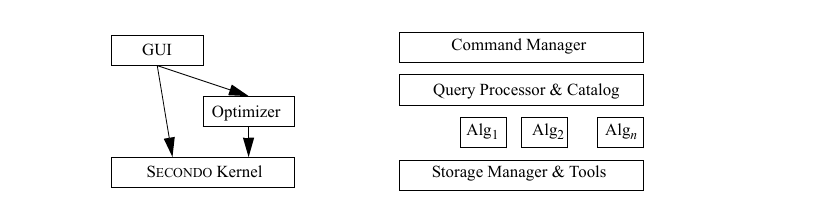
\includegraphics[width=0.75\textwidth]{Bilder/secondo.png}
	\caption{SECONDO Komponenten und Architektur des Kernels \parencite{Gueting2010}.}
	\label{img:secondo}
\end{figure}

Abstract Data Types (\Fb{ADT}) fassen Datentypen mit dazugehörigen Operationen zusammen und ermöglichen es, beispielsweise räumliche Datentypen gemeinsam mit den notwendigen Operationen zu entwerfen, ohne sich bereits über die Implementierung und detaillierte Struktur der Datentypen Gedanken zu machen. {\textcite[S. 75ff]{Rigaux2001}} beschreiben, wie ADTs für räumliche Datentypen entworfen werden können. \Fb{Secondo} setzt dieses Konzept weitestgehend um. Die \Fb{SpatialAlgebra} bietet darüber hinaus ein ausreichendes Set topologischer Prädikate, um hinreichend räumliche Beziehungen zwischen Punkten, Sets von Punkten, Linien und Regionen/Polygonen zu beschrieben.

Wichtig für die von mir zu entwickelnde Algebra sind mehrere Bestandteile von \Fb{Secondo}. Die \Fb{RelationalAlgebra} stellt das relationale Datenmodell inklusive des Datentyps Tupel und Persistierungsstrukturen für Tupel zur Verfügung. Die Stromverarbeitung ermöglicht es, große Sätze von Daten in einer Pipeline zu verarbeiten; in meinem Fall in Tupelströmen. Fake Large Objects (\Fb{FLOBs}) ermöglichen es, Instanzen von Typen mit variabler Größe zu implementieren, indem ein Objekt abhängig von der Größe entweder Teil des Tupel ist oder separat gespeichert wird. Unter Anderem für die Implementierung räumlicher Datentypen sind solche Möglichkeiten essentiell. Für einen schnellen Zugriff werden zum Beispiel räumliche Datentypen variabler Größe durch ihre minimale Bounding Box direkt im Tupel repräsentiert. Ein \Fb{FLOB} hat also immer eine Repräsentation klar begrenzter Größe in dem Teil des Tupels, der immer in den Hauptspeicher geladen wird, wenn auf den Tupel zugegriffen wird \parencite{Gueting2010}.

Der \Fb{Command-Manager} bietet neben einer dem \Fb{SQL}-Standard entsprechenden Abfragesprache eine zweite, \Fb{executable} Abfragesprache genannte Sprachebene, die in ihrer Abstraktion zwischen \Fb{SQL} und einer Programmiersprache wie \Fb{C++} steht. Mit dieser Abfragesprache können Anfragen direkt an den Kernel gestellt werden, und dementsprechend steht nur auf dieser Ebene der volle Funktionsumfang des Kernels zur Verfügung. Allerdings ist \Fb{SQL} deutlich einfacher zu benutzen \parencite{Gueting2010}. 

Bereits jetzt sind Ansätze paralleler Datenverarbeitung in \Fb{Secondo} integriert. Die \Fb{DistributedAlgebra} \parencite{Nidzwetzki2017} ermöglicht eine Verarbeitung eines verteilten Anfrageprozesses, indem mehre \Fb{Secondo}-Instanzen auf einem oder mehreren Computern genutzt werden. Anfragen werden auf die Instanzen partitioniert und nach der Verarbeitung die Teilergebnisse wieder zusammengeführt. Einen Schritt weiter geht die erst kürzlich implementierte \Fb{ParThread}-Algebra, die eine Parallelisierung innerhalb einer Instanz für den Benutzer verborgen vornimmt, indem Operatoren für die Parallelisierung zur Verfügung gestellt werden und der Operatorenbaum möglichst optimal für eine parallele Verarbeitung umgeformt wird.

\subsection{Multiprozessorsysteme}

Für ein späteres Verständnis des Performance-Verhaltens der von mir entworfenen Operatoren ist ein grundlegendes Verständnis der Funktionsweise und des Aufbaus von Mehrkernprozessoren notwendig. Multiprozessorsysteme grenze ich hier ab von verteilten Systemen. Während in ersteren die verschiedenen Kerne bzw. Prozessoren in einem Computer integriert sind und sich den Speicher wie auch die anderen Komponenten teilen, bestehen verteilte Systeme aus unabhängigen Computern, die über ein Netzwerk miteinander verbunden sind. Man spricht hier auch von enger und loser Kopplung. Dementsprechend sind in verteilten Systemen die Kommunikationskosten zentral für die Bestimmung der Performance. Als weitgehend identisch betrachte ich für meine Fragestellung Mehrkern- und Mehrprozessorsysteme. Einziger Unterschied ist meist die Aufteilung des Caches auf mehrere Prozessoren bei Mehrprozessorsystemen, aber auch einzelne Komponenten können unabhängig voneinander sein. In älterer Literatur wird meist von Mehrprozessorsystemen gesprochen, da Mehrkernprozessoren eine relativ neue Entwicklung sind. Eingehen werde ich hier nur auf Mehrkernprozessoren.

In der Flynn’schen Taxonomie paralleler Architekturen, die globale Kontrolle und resultierende Daten sowie Kontrollflüsse zwischen den Prozessen betrachtet, entsprechen Mehrkern- und auch Mehrcomputersysteme einer Multiple Instruction, Multiple Data (MIMD) Rechnerarchitektur \parencite[S. 10f]{Rauber2013}. Andere Architekturen sind beispielsweise für die parallele Bearbeitung von Bilddaten auch in Desktop-Computern relevant.

Ab 2005 war eine Leistungssteigerung von Einkernprozessoren wegen der entstehenden Abwärme nicht mehr in großem Umfang technisch möglich. Anstatt vor allem auf die Steigerung des Prozessortakts zu setzen, wurden ab dieser Zeit Prozessoren mit mehreren unabhängigen Einheiten, Kerne genannt, entwickelt, die ab 2009 Standard in Desktopcomputersystemen wurden. Die CPU-Kerne haben eigene Registersätze und arithmetisch-logische Einheiten (\Fb{ALU}), nur der Bus und einige Caches werden von mehreren Kernen geteilt. Die Leistungssteigerung von Computerprogrammen wurde dementsprechend abhängig von einer parallelen Ausführung von Programmeinheiten. Standard-Desktopprozessoren unterliegen einem hierarchisches Design. Für die Performance von Multiprozessor-Algorithmen ist eine optimale Nutzung der Kern-spezifischen L1/L2-Caches und dem geteilten L3-Cache wichtig \parencite{Rauber2013}. Der Cache enthält exakte Kopien von Daten und Befehlssätzen aus dem Hauptspeicher, die besonders häufig genutzt werden. Der L1-Cache ist am schnellsten, aber meistens nicht sehr groß. Befehls- und Datencache sind hier getrennt. In einigen Systemen hat nicht jeder Kern die vollständige Funktionalität eines Prozessors, sondern bestimmte Ressourcen, wie die Gleitkommaeinheit, werden zwischen mehreren Kernen geteilt. Beispielsweise sind in der AMD-FX-Architektur zwei Kerne mit je eigener Integereinheit und eigenem L1-Cache zu einem Modul mit geteilter Gleitkommaeinheit und geteiltem L2-Cache zusammengefasst. Hyperthreading ist eine Technik, mehrere Threads auf einem Kern gleichzeitig auszuführen und so zu koordinieren, dass die Ausführung schneller ist, als wenn die Threads seriell ausgeführt würden. Diesen Ausführungen folgt, dass die Performance auch vollständig unabhängiger Threads ohne Overhead nicht unbedingt linear wächst bei einer steigenden Anzahl von Kernen, da sich Kerne teils Ressourcen teilen.

Parallele Ausführungen kann es mit unterschiedlicher Kopplung geben. Man unterschiedet zwischen Threads und Prozessen. Threads sind über einen eigenen Kontrollfluss definiert. Sie haben einen unabhängigen Registersatz inkl. Instruction Pointer, einen eigenen Stack, aber im Gegensatz dazu verfügen Prozesse über einen eigenen Adressraum \parencite[S. 95]{Rauber2013}. Die meisten Betriebsmittel werden von allen Threads gemeinsam verwendet. Durch die gemeinsame Nutzung von Betriebsmitteln kann es auch zu Konflikten kommen. Diese müssen durch den Einsatz von Synchronisationsmechanismen aufgelöst werden.

\subsection{Parallele Algorithmen}

Warum aber wird eine Parallelisierung nicht automatisch vorgenommen? Die \Fb{ParThreaded}-Algebra, die bereits in \Fb{Secondo} implementiert worden ist, verfolgt beispielsweise
diesen Ansatz: Sie stellt Operatoren zur Verfügung, um bereits implementierte Singlethread-Operatoren parallel ausführen zu können. Am Beispiel eines parallelen (internen) Merge-Sort zeigen {\textcite{McCool2012}}, warum es oft besser ist, einen neuen parallelen Algorithmus zu suchen anstatt einen seriellen zu parallelisieren. Meistens lohnt es sich also, explizit parallele Operatoren zu entwerfen.

{\textcite[S.104]{Rauber2013}} unterscheidet parallele Programmiermodelle nach folgenden Kriterien:

\begin{itemize}
	\item Befehlsebene, Ebene des Befehlsblocks, prozedurale Ebene oder parallele Schleife
	\item implizite oder explizite Parallelität
	\item synchron oder asynchron
	\item Kommunikationsmuster: explizite Kommunikation oder geteilte Variablen
	\item Synchronisationsmechanismen
\end{itemize} 

Greifen sogenannte kritische Bereiche auf gleiche Daten zu, müssen die Zugriffe synchronisiert werden, da es zu Deadlocks oder zu kritischen Wettlaufsituationen (\Fb{race conditions}) kommen kann. Von einem Deadlock spricht man, wenn zwei Prozesse auf jeweils eine Sperre warten, aber die genau andere Sperre besitzen. So kommt es zu einer Verklemmung. Sofern in parallelen Algorithmen auf gemeinsame Daten zugegriffen wird, kann die Ausführungsreihenfolge das Ergebnis bestimmen, was als Wettlaufsituation bezeichnet wird. Locks stellen Sperren zur Verfügung, sorgen also dafür, dass eine Aktion atomar ist, und Mutexe sichern den ausschließlichen Zugriff auf kritische Daten, garantieren also, dass ein Zugriff atomar stattfindet \parencite{Rauber2013}. Eine Kommunikation zwischen den Threads findet entweder über Nachrichten oder globale Variablen statt. Mit diesen Mitteln kann eine Prozesssynchronisation vorgenommen und sichergestellt werden, dass die einzelnen Aktionen der Threads konsistenzerhaltend sind.

Die Entwicklung einer parallelen Problemlösung wird beeinflusst von der Struktur des Problems und der Daten. Wenn sich ein Problem in Teilprobleme ohne funktionale Abhängig"-keit zerlegen lässt, spricht man von inhärentem Parallelismus \parencite[S. 321f]{Bengel2008}. Da in diesem Fall wenig Kommunikation zwischen den Prozessen notwendig ist, wird theoretisch ein nahezu linearer Performancegewinn ermöglicht. Eine Zerlegung in Teilprobleme kann über eine Aufteilung der Daten stattfinden, also über eine Partitionierung. Bei einer funktionalen Zerlegung eines Problems in mehre Arbeitsschritte, die nacheinander ausgeführt werden, spricht man von Pipelining \parencite[S. 324]{Bengel2008}. Verteilte beziehungsweise parallele Algorithmen haben im Gegensatz zu Zentralen keinen globalen Zustand und keine gemeinsame Zeit. Dementsprechend kann es zu unvorhersehbaren Abläufen kommen. Eine Rechenlastverteilung kann statisch oder dynamisch vorgenommen werden \parencite{Bengel2008}.

Im Folgendem beschreibe ich einige Architekturmuster, die häufig im Entwurf paralleler Problemlösungen Anwendung finden. Im Fork-Join-Muster werden Threads für bestimmte Aufgaben erzeugt und hinterher wieder zusammengefügt \parencite[S. 109]{Rauber2013}. Im Master-Worker-Schema verteilt ein Master Teilbereiche von Daten an mehrere Worker und sammelt die Ergebnisse wieder ein. Der Master übernimmt also ein Scheduling im Gegensatz zum Fork-Join-Muster, welches ohne eine zentrale Instanz auskommt. Der Weg von einer Zerlegung eines Problems zu einer Allokation der Teilprobleme auf Prozessoren kann in vier Schritten beschrieben werden: Partitionierung, Auslegung der Kommunikation, Agglomeration (die Gruppierung von Aufgaben und Daten) und Mapping (Zuweisung von Aufgaben an Prozesse). Unterschieden werden hier Ansätze mit viel oder wenig Kommunikation und Parallelisierung \parencite[S. 326f]{Bengel2008}. Im bereits erwähnten Pipelining-Architekturmuster findet eine funktionale Zergliederung des Problems statt und die Daten werden nacheinander in einer Kette von Threads verarbeitet \parencite[S. 111]{Rauber2013}. Im Producer-Consumer-Muster gibt es mehrere Threads, die Daten erzeugen, und mehrere, die Daten erhalten. Eine Kommunikation findet über Buffer statt \parencite[S. 112]{Rauber2013}.

In der Performance-Analyse wird unterschieden zwischen Kosten, Beschleunigung und Effizienz unter Verwendung des PRAM-Modells (paralleler RAM). Das Performance-Verhalten bei wachsender Anzahl von Prozessoren wird Skalierbarkeit genannt \parencite{Rauber2013}. Beschleunigung beschreibt den Faktor, um den eine Ausführung auf mehreren Workern schneller wäre als auf einem, Effizienz die Beschleunigung pro Worker \parencite[S. 56]{McCool2012}. Fallstricke paralleler Programmierung liegen in einer gedrosselten Skalierung, also einem nicht-linearen Anstieg der Performance mit der Anzahl genutzter Kerne verursacht unter anderem durch eine unausgeglichene Lastenverteilung oder durch einen großen Overhead für die Verwaltung der parallelen Prozesse \parencite[S. 74]{McCool2012}.

\subsection{Parallele Datenbanksysteme}
\label{P_DBS} 

Trotz einer gewissen Verwandtschaft müssen von den parallelen Datenbanksystemen verteilte Datenbanksysteme abgegrenzt werden, auch wenn es Überschneidungen in den angewandten Techniken gibt. Parallele Datenbanksysteme sind räumlich integriert und die Parallelisierung ist innerhalb einer Instanz eines Datenbanksystems implementiert. In verteilten Datenbanksystemen findet eine Parallelisierung zwischen verschiedenen Instanzen unter Umständen auch heterogenen Datenbanksysteme statt, die häufig räumlich getrennt sind, aber auch innerhalb eines Rechner ablaufen können. Dementsprechend werden in beiden Typen von Datenbanksystemen Daten durch verschiedenen Prozesse gleichzeitig verarbeitet, nur sind die Kommunikationskosten in verteilten Systemen deutlich höher, da die Kommunikation über externe Schnittstellen der Datenbanksysteme und meist über Netzwerkverbindungen stattfindet. Eine Kommunikation über geteilte Bereiche des Hauptspeichers ist wesentlich effizienter. Die Kopplung in verteilten Systemen wird als lose bezeichnet. Dem entgegenstehend sind parallele Datenbanksysteme eng gekoppelt.

Die Architekturen paralleler Datenbanksysteme werden danach untergliedert, ob diese sich gemeinsamen Speicher bzw. Permanentspeicher teilen: Es können drei grundsätzliche Architekturen unterschieden werden, nämlich shared-all-Architekturen, Architekturen mit nur geteiltem Permanentspeicher oder nur geteiltem Speicher \parencite{Yu1998}. Datenbanksystemen, die auf Desktop- oder Serversystemen laufen, gehören meist der shared-all Architektur an oder nutzen für jeden Prozess gemeinsamen Speicher, aber unterschiedliche permanente Speicher. In dieser Arbeit werde ich mich auf eine shared-all-Architektur beschränken. Allerdings wäre durch eine parallele Nutzung mehrerer Festplatten ein deutlicher Performancegewinn denkbar, da häufig die I/O-Operationen den Performance-Flaschenhals darstellen.

Parallelität kann in Datenbanken auf verschiedene Art und Weise erreicht werden. Unterschieden werden kann eine Parallelität zwischen Transaktionen, zwischen Operationen, einer direkten Implementierung paralleler Operationen und einem parallelem Zugriff auf gespeicherte Daten \parencite{Reuter1999}. \textcite [S. 1]{Yu1998} unterscheiden zwischen Inter- und Intra-Operator-Parallelität. Auf der Ebene der Architektur grenzen \textcite{Yu1998} unabhängige Parallelität, Pipelined-Parallelität und partitionierte Parallelität voneinander ab. Während in der unabhängigen Parallelität verschiedene Aufgaben gleichzeitig ausgeführt werden, findet in einer Pipeline ein Datenfluss durch mehrere funktional verschiedene Operationen statt und in der partitionierten Parallelität werden die Daten aufgeteilt in Pakete, die von gleichen Operationen verarbeitet werden \parencite{DeWitt1992}.

Die Effektivität von Multithreading-Algorithmen hängt davon ab, inwieweit eine gleich"-mäßige Lastverteilung gelingt und der Koordinierungs- und Synchronisierungs-Overhead minimal gehalten werden kann \parencite{Lakshmi1990}. Die Kosten für parallele Datenbankoperationen werden nach I/O-Kosten, CPU-Kosten und Kommunikationskosten unterschieden \parencite [S. 23]{Yu1998}. Kommunikationskosten und das notwendige Scheduling, das heißt die Aufteilung der Daten und Zusammenführung der Ergebnisse, sind dafür verantwortlich, dass die Performance von parallelen Operatoren nicht mit der Threadzahl linear wächst. Ein Load Balancing kann statisch und dynamisch vorgenommen werden, wobei ein dynamisches Load Balancing zwar besser auf unterschiedliche Charakteristika der zu prozessierenden Daten reagieren kann, aber den Overhead erhöht. Allerdings gibt es meist Heuristiken für eine gute Datenpartitionierung.

Wichtig für die Parallelität von Datenbankabfragen ist die Partitionierung der Daten. Hier sind vor allem drei Strategien relevant: Round Robin verteilt die Daten abwechselnd gleichmäßig auf die Prozesse, eine Bereichspartitionierung unterteilt den Wertebereich in Segmente und eine Hashpartitionierung verteilt nach einer Hashfunktion in Buckets \parencite{Yu1998}. Sowohl eine Bereichs- als auch eine Hashpartitionierung kann, insbesondere wenn keine Statistiken über die Daten vorliegen, zu einer Ungleichverteilung führen. Dagegen führt Round Robin zwar zu einer gleichmäßigen Verteilung, allerdings nicht zu unterschiedlichen Eigenschaften der Daten innerhalb einer Partition, die eventuell für eine Implementierung ausgenutzt werden können. Deutlich komplexer ist eine Partitionierung von Nicht-Standard-Datentypen. Von Bedeutung für meine Fragestellung sind vor allem räumliche Datentypen. Auf Ansätze zu deren Partitionierung werde ich in \autoref{Spatial Join} detailliert eingehen. 


\subsection{Parallele Datenbankoperatoren}

\subsubsection{Sort}
\label{Sort} 

Damit Sortierverfahren für den Einsatz in Datenbanksystemen infrage kommen können, müssen sie in der Lage sein, Daten auch zu sortieren, wenn sie nicht vollständig in den Hauptspeicher passen, also externe Sortierverfahren sein. Das bekannteste dieser externen Sortierverfahren ist Merge-Sort. Das optimale Laufzeitverhalten für externe Sortierverfahren ist $ n \log n $ mit $n = Anzahl~der~Tupel$. Für eine Parallelisierung ist also $ \frac{n \log n} {k} $ mit $k = Anzahl~der~Threads$ zu erwarten, sofern kein zusätzlicher Verwaltungsaufwand anfällt. Eingehen werde ich hier nur auf Record-basierende Sortierverfahren, die ganze Tupel im Gegensatz lediglich zu Schlüsseln sortieren (und auch nur Schlüssel ausgeben) \parencite{Salzberg1990}. Unter den externen Sortierverfahren eigenen sich vor allem zwei Ansätze für eine parallele Implementierung: vom Merge-Sort abgeleitete Verfahren und Sortiernetzwerke. {\textcite[S. 831ff]{Taniar2000}} stellen in einem Übersichtsartikel fünf Algorithmen vor, die sich besonders gut für eine parallele Implementierung eignen. {\textcite[S. 9ff] {Bitton1984}} ergänzen darüber hinaus in ihrer Taxonomie paralleler Sortierverfahren die Sortiernetzwerke, als deren Beispiel ich auf das Bitonic-Sortiernetzwerk eingehen werde.

\begin{figure}
	\centering
	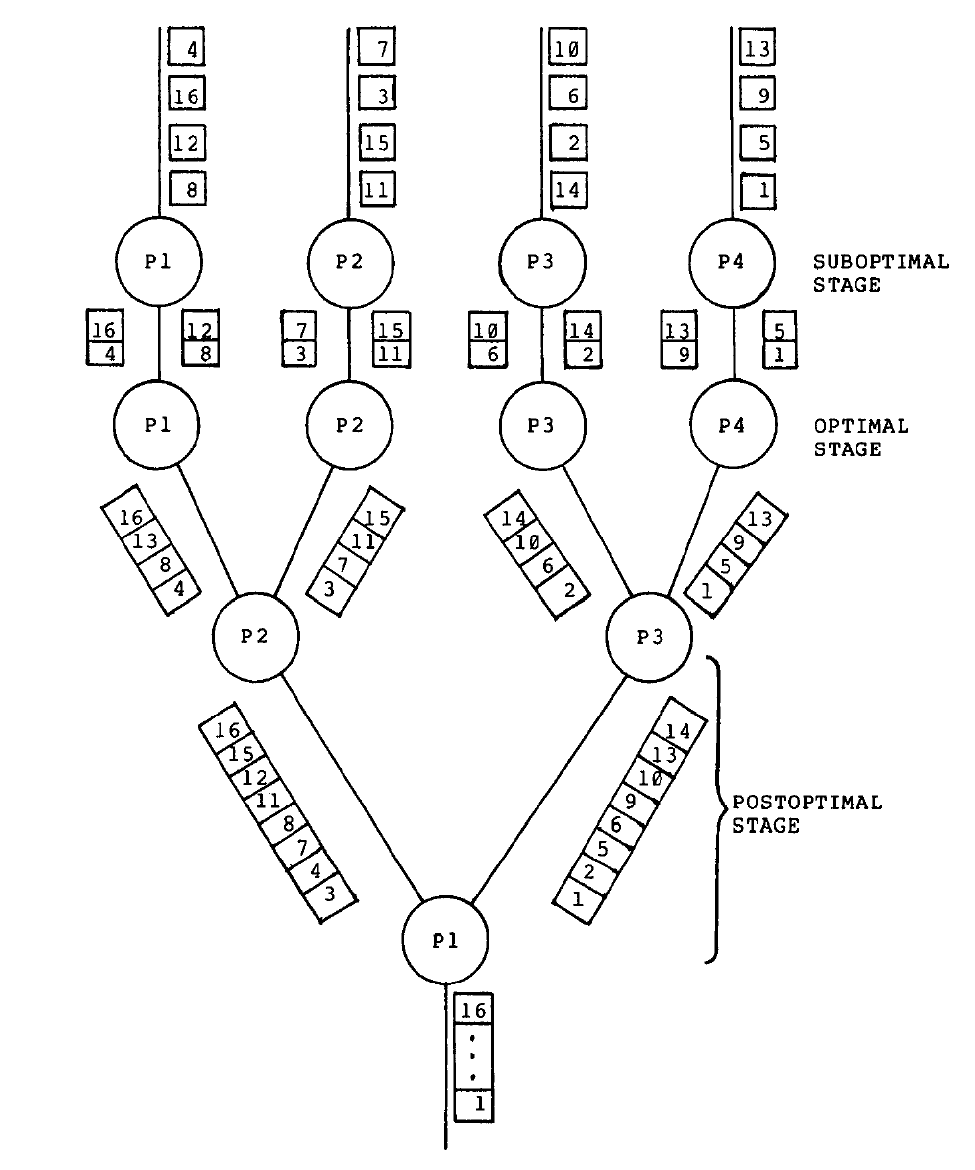
\includegraphics[width=0.5\textwidth]{Bilder/b-merge-sort.png}
	\caption{Paralleler binärer Merge-Sort \parencite[S. 334]{Bitton1983}.}
	\label{img:bMergeSort}
\end{figure}

Parallele Merge-All-Sorts \parencite[S. 831f]{Taniar2000} setzen sich aus zwei Phasen zusammen. In einer Sortierphase wird mit einem seriellen internen Sortierverfahren in den einzelnen Threads sortiert. Dem folgend finden die Merge-Schritte statt, wobei nach jedem Schritt weniger Threads benötigt werden, bis der finale Merge-Schritt nur noch von einem Thread ausgeführt wird. Nachteil dieses Verfahrens ist ein sehr umfangreicher letzter Schritt, der nur in einem Prozess stattfinden kann. Im Unterschied dazu teilt der binäre Merge-Sort \parencite[S. 832f]{Taniar2000} die Merge-Phase in eine Pipeline von Merge-Schritten auf, in der je zwei Läufe zusammengefügt werden. Die Idee der parallelen Version eines binären Merge-Sort \parencite[S. 833]{Taniar2000} ist es, dass die Merge-Phase als Strom konzipiert wird und dementsprechend die Kerne auch in dieser Phase deutlich besser ausgenutzt werden. Ein anderer Ansatz ist, mithilfe einer bereichsbasierten Aufteilung (siehe \autoref{P_DBS}) zwischen intermediären und finalen Merge-Schritten zu gewährleisten, dass in jedem Merge-Schritt gleich viele Kerne genutzt werden. Dagegen reduziert der parallele Merge-All-Sort \parencite[S. 833f]{Taniar2000} die Höhe des Merge-Baumes, indem der Sortierprozess auf zwei Schritte reduziert wird: eine lokale Sortier- und eine finale Merge-Phase. Der parallele verteilende Sort arbeitet mit einer bereichsbasierenden Aufteilung und einem abschließenden Sortierschritt. Bei den Sortierverfahren, die eine bereichsbasierende Aufteilung nutzen, ist das zentrale Problem, in Näherungsverfahren oder genau berechnet die beste Aufteilung zu bestimmen \parencite{Lu1994, Iyer1989}. Bei unbekannten Relationen bieten sich also eher Verfahren an, die eine zufällige Partitionierung, Round Robin genannt, voraussetzen.

Detailliert werde ich \textcite[S. 333ff]{Bitton1983} folgend auf den binären Merge-Sort eingehen, der in drei Phasen abläuft (siehe \autoref{img:bMergeSort}). Die sogenannte suboptimale Phase reduziert die Anzahl der Läufe so lange, bis so viele Läufe vorhanden sind, wie Kerne genutzt werden, also in jedem Thread einer. In der optimalen Phase gibt es für jeden Kern genau einen Lauf und in der postoptimalen Phase wird solange verschmolzen, bis nur noch ein Lauf vorhanden ist. In dieser Phase gibt es zwar weniger Läufe als Kerne genutzt werden, aber über Pipelining wird trotzdem die Parallelität optimal verwendet, anders als in einigen trivialen Ansätzen \parencite{Yu1998}, die kein Pipelining nutzen und so in der postoptimalen Phase in jedem Schritt die Parallelität reduzieren. Die Laufzeit dieses Ansatzes ist wie folgt:

\[
\underbrace{\frac{n}{2p} \log \left( \frac{n}{2p} \right)}_{suboptimal} + \underbrace{\frac{n}{2p}}_{optimal} + \underbrace{\log p - 1 + \frac{n}{2}}_{postoptimal} \:
\begin{cases}
n: \text{Anzahl von Tupeln}\\
p: \text{Anzahl von Threads}
\end{cases}
\]

Allerdings nutzt der bisher beschriebene binäre Merge-Sort den vorhandenen Arbeitsspeicher nicht aus. Deshalb bietet es sich an, die Läufe im Arbeitsspeicher vorzusortieren, um die I/O-Belastung zu reduzieren. Der Fast-Sort-Algorithmus \parencite{Tsukerman1986, Salzberg1990} schlägt hier ein Sortieren über Replacement Selection \parencite[vgl.][]{Knuth1973} vor, da dieses Sortierverfahren längere Läufe erzeugen kann, als in den Hauptspeicher passen würden und eine gleichzeitige Ein- und Ausgabe möglich ist, die das Pipelining optimieren kann. Eine Verteilung auf die anfänglichen Threads findet nach Round-Robin statt.

\textcite{Salzberg1990} betont, dass die Phasen, die die Läufe sortieren, vor allem durch die CPU limitiert sind, aber die Merge-Phasen durch die Geschwindigkeit des Zugriffs auf den permanenten Speicher, da die einzelnen Läufe, sofern größer als der Hauptspeicher, auf Festplatten ausgelagert werden müssen. Dementsprechend lohnt es sich, jedem Lauf eine eigene Festplatte zuzuweisen. \textcite{Hao2009} erläutert die optimale Verwendung des Prozessor-Caches.

\begin{figure}
	\centering
	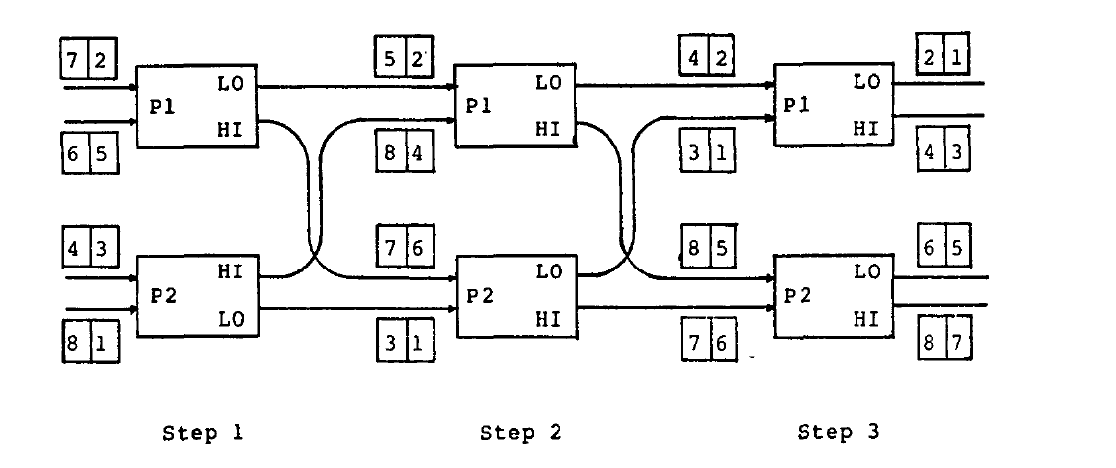
\includegraphics[width=0.75\textwidth]{Bilder/bitonic_block.png}
	\caption{Block Bitonic Sortiernetzwerk mit zwei Prozessoren \parencite[S. 335]{Bitton1983}.}
	\label{img:bitonic}
\end{figure}

Das Bitonic-Sortiernetzwerk \parencite[S. 335f]{Bitton1983} hat den Vorteil, dass in jedem Schritt die gleiche Anzahl von Kernen genutzt wird. Jeder Schritt besteht aus parallelen Modulen, die Werte vergleichen, in zwei Gruppen aufteilen und dann entsprechend dem in \autoref{img:bitonic} dargestellten Muster in einen nächsten Schritt transportieren. Der Algorithmus sortiert $n$ Werte mit $\frac {n} {2} $ Vergleichs-/Austauschmodulen in $\frac{1}{2} \log n (\log n +1)$ Schritten. Allerdings kann, wenn nicht genügend Module parallel ausgeführt werden können, innerhalb eines Moduls ein nach Bedarf internes oder externes Sortierverfahren angewendet werden. In diesem Fall wird die kleinere bzw. größere Hälfte einer sortierten Folge weitergereicht. Module können als Prozessoren/Kerne begriffen werden. Sortiernetzwerke stellen also eine Alternative dar zum Ansatz des Pipelinings. Eine Alternative zum Sortieren innerhalb der Module ist es, in einer vorbereitenden Phase beispielsweise mit einem parallelen 2-Wege-Merge-Sort bis zur Blockgröße, die für ein Sortiernetzwerk mit den zur Verfügung stehenden Prozessoren ausreicht, zu sortieren. Für ein Sortiernetzwerk aus vier Modulen wären zum Beispiel acht sortierte Läufe notwendig. Dieses Verfahren wird Block Bitonic Sortiernetzwerk genannt \parencite[S. 335]{Bitton1983}  Die Gesamtkosten setzen sich aus den Kosten für das Bitonic-Sortiernetzwerk und den vorbereitenden Schritt zusammen -- entsprechend \textcite[S. 335]{Bitton1983} wurde ein 2-Wege-Merge-Sort berücksichtigt, der bei relativ kleiner Threadzahl und großen Relationen doppelt so schnell wie die Anwengung eines Bitonc-Sortiernetzwerk in mehreren Phase ist:

\[
\left[ \log _2 (\frac {n} {2 p}) + \frac {\log _2 ^2 2 p - \log _2 p} {2} \right] ( \frac {n}{2 p}) C _{p} ^{2}\:
\begin{cases}
n: \text{Anzahl von Tupeln}\\
p: \text{Anzahl von Prozessoren}\\
C: \text{Kosten für einen Vergleich}
\end{cases}
\]

{\textcite{Menon1986}} schlägt eine modifizierte Version des Block-Bitonic-Sort als externen parallelen Algorithmus vor, der Bitonic-Sort als internen Algorithmus nutzt und mit Pipelining kombiniert. Pipelining beschleunigt den Merge-Schritt, aber nicht Bitonic-Sort selbst. Das interne Sortieren bringt einen Performance-Vorteil gegenüber mehrfachem Verschmelzen. Pipelining lohnt sich vor allem, wenn es eine große Anzahl von Merge-Schritten gibt.

Untersuchungen von {\textcite{Bitton1984}} legen nahe, dass sich für externes Sortieren der parallele binäre Merge-Sort mit Pipelining am besten eignet. Dagegen stellt {\textcite{Menon1986}} fest, dass der binäre Merge-Sort-Algorithmus nur bei großem $n$ und einer kleiner Kernzahl schneller als der Block-Bitonic-Sort ist. In modernen Desktopsystem ist dies aber meistens der Fall.

\subsubsection{Equi-Join}
\label{Equi Join} 

Joins gehören zu den teuersten Operatoren in Standard-Datenbanken und sind die einzigen Operatoren, die es erlauben, mehrere Relationen zu verbinden. Dementsprechend werden sie sehr häufig angewandt und die Diskussion um mögliche Performancegewinne durch eine Parallelisierung ist umfangreich \parencite{Richardson1987, Valduriez1984, Schneider1989, DeWitt1985, Lu1994}. Die wichtigsten Join-Operatoren sind der Nested-Loop-Join, Sort-Merge-Join, die Gruppe der Hash-Joins und Hash-partionierenden Joins \parencite{Mishra1992, Lu1994}, auf deren parallele Implementierung ich im Folgenden eingehen werde. Die erste der beiden zu verschmelzenden Relationen nenne ich R-Relation, die Zweite S-Relation.

Da sich allgemein Schleifen sehr einfach parallelisieren lassen, liegt für den Nested-Loop-Join ein einfacher paralleler Algorithmus vor. Allerdings ist der Nested-Loop-Join in seiner seriellen Implementierung sehr teuer. Insbesondere wenn die Selektivität gering ist, sind die meisten Vergleiche nicht notwendig. Deswegen lohnt sich der Nested-Loop-Join auch in einer parallelen Variante nur, wenn entweder ein Full-Outer-Join vorgenommen wird oder fast alle Tupel miteinander verbunden werden. Die Komplexität beträgt $ O(n m) $, also im parallelen Fall $ O( \frac {n m} {p} )$ ($m,n$: Tupel; $p$: Anzahl Threads) \parencite[S. 72]{Mishra1992}. Im Gegensatz zu den Join-Algorithmen, die Hashing nutzen, ist der Nested-Loop-Join und auch der Sort-Merge-Join in der Lage, Non-Equi-Joins vorzunehmen, zumindest in der Grundform. 

Der Sort-Merge-Join gehört zu den effizienten Algorithmen in Singlethread-Datenbank"-systemen. Die Idee ist es, zuerst beide Relationen, die verschmolzen werden sollen, zu sortieren, um sie dann einfach verbinden zu können \parencite[S. 149]{Lu1994}. Wie sich der Sortierschritt parallelisieren lässt, habe ich bereits erläutert (siehe \autoref{Sort}). Allerdings ist es schwer, den Merge-Schritt zu parallelisieren. Sort-Merge-Joins verbessern sich nur schwach mit der Anzahl der Prozessoren \parencite{Yu1998}; ein Ansatz einer weitreichenden Parallelisierung wird mit der Fragment- und Replicate-Methode vorgestellt \parencite {Richardson1987} Die beiden zu verschmelzenden Relationen werden partitioniert. Hier gibt es zwei Möglichkeiten: Jede sortierte Partition der Basisrelation aus R wird mit jeder Partition aus S mit Merge-Join verbunden oder die kleinere Relation wird zuerst verschmolzen. Dieser Ansatz ermöglicht eine stärkere Parallelisierung, hat aber Probleme in der Performance, da er eine Annäherung an einen Loop-Join darstellt. In einer anderen Methode findet eine Bereichs-Partitionierung in $k$ Fragmente statt. Die entsprechenden Paare können dann verschmolzen werden. \textcite{Iyer1989} schlagen ein Verfahren zur Ermittlung einer idealen Partitionierung vor. Die Sort-Merge-Join-Algorithmen erhalten die Reihenfolge der Relationen und haben Vorteile, wenn Relationen bereits sortiert sind bzw. ein Index vorliegt.

Hash-basierte Join-Algorithmen sind besser geeignet für eine Parallelisierung. Sie sind aber nur in der Lage, einen Equi-Join bezüglich eines Joinattributes zu berechnen. Beide Phasen, die Partitionierungs-Phase und die Join-Phase, können parallelisiert werden. Die Grundidee ist, beide Relationen mithilfe einer Hash-Funktion in Buckets aufzuteilen und nur Tupel zu testen, die sich im gleichen Bucket befinden. Die Komplexität der Grundform beträgt $O(m + n)$, da jede Relation nur einmal gescannt werden muss, sofern die Hashfunktion und die Verteilung ideal ist. Für eine Shared-all-Architektur bietet sich eine globale Hashtabelle an. Alle Singlethread-Hash-Join-Algorithmen können auf diese Art und Weise parallelisiert werden. Probleme können bei ungünstigen Hash-Funktionen mit ungleicher Verteilung und beim Überlauf der Hash-Tabellen auftreten. Auf diese Problematik werde ich später eingehen. Grace- und Hybrid-Hash-Join-Verfahren eignen sich besonders gut für eine Parallelisierung \parencite{DeWitt1985}. Eine mögliche Optimierung stellen Bit-Array-Datenstrukturen dar, um zu markieren, dass für ein Joinattribut ein Partner existiert \parencite{Valduriez1984}. Im Folgenden stelle ich die wichtigen Hash-Join-Algorithmen kurz vor:

\begin{itemize}
	\item Simple Hash: Partitioniere weiter auf jedem Kern und speichere nicht behandelte Tuple temporär \parencite{Lu1994}.
	\item Grace-Join: Phase 1 + 2: Beide Relationen werden partitioniert. In einer finalen Phase findet das Matching statt. Jeder Behälter muss in den Arbeitsspeicher passen. Der fundamentale Unterschied zu Sort-Merge-Join und Simple Hash-Join ist die zweifache Partitionierung bei der Bucket-Formung und bei der Bucket-Verschmelzung \parencite{Schneider1989}.
	\item Hybrid-Join: Versucht I/O-Verkehr zu minimieren, indem beide Phasen des Grace-Joins nicht völlig getrennt sind. In jedem Kern findet eine Join-Phase direkt im Hauptspeicher in drei Phasen statt und versucht dabei, einen Overflow zu vermeiden \parencite{Schneider1989}:
	\begin{enumerate}
		\item R in $n$ Buckets. Erstes Bucket wird direkt intern verschmolzen.
		\item S in $n$ Buckets. Wieder erstes Bucket direkt im Speicher und testen auf Joins (parallel).
		\item Der Rest wird verschmolzen.
	\end{enumerate}
\end{itemize}

Hashtabellen müssen in den Speicher passen, da sonst in der Matching-Phase der Join-Operatoren teure I/O-Operationen anfallen. Prinzipiell werden zwei Lösungsansätze diskutiert: Es werden mehr Partitionen verwendet als theoretisch notwendig sind, um einer ungleichen Datenverteilung vorzubeugen. Allerdings sind für diesen Ansatz Kenntnisse über die Relationen notwendig und eine sinnvolle Wahl der Anzahl von Partitionen ist nur durch einen Optimierer möglich. {\textcite{Lu1994}} diskutieren, welche Statistiken über die Verteilung innerhalb der Relationen notwendig sind und wie das Load Balancing gestaltet werden soll, also ob eine First-fit- oder Best-fit-Strategie gewählt, aber auch, ob das Load Balancing dynamisch oder statisch vorgenommen werden soll. Ein anderer Ansatz ist das nachträgliche Aufteilen der Hashtabellen \parencite{Mishra1992}. Das Overflow-Problem der Buckets kann durch einen rekursiven Partitionierungsprozess gelöst werden \parencite{DeWitt1985}.

Ein weiterer Faktor für die Performance ist die Task-Generierung, also die Frage, ob Subrelationen überlappend oder vollständig geteilt werden und wie viel Tasks erzeugt werden sollen. Beim Grace-Join-Algorithmus beispielsweise kann es sinnvoll sein, mehrere Threads pro zur Verfügung stehenden Kern zu verwenden \parencite{Lu1994}. 

Hash-partitionierende Joins folgen einem Divide- und Conquer-Ansatz und kombinieren die Idee der Hash-Joins mit der Performance von Sort-Merge-Sorts in ihrer Singlethread-Version. Damit wird die Schwierigkeit umgangen, Sort-Merge-Joins zu parallelisieren \parencite[S. 75ff]{Mishra1992}. Die Idee ist simpel: Beide Relationen werden mit einer Hashfunktion auf die Threads verteilt. Dem folgend findet in jedem Thread lokal parallel ein Sort-Merge-Join statt \parencite{Richardson1987}. Wenn die R-Relation größer ist als der Arbeitsspeicher, gibt es mehrere Läufe \parencite{Lu1990}.

In einem detaillierten experimentellen Performance-Vergleich paralleler Join-Imple"-men"-tie"-rungen stellen {\textcite{Valduriez1984}} fest, dass Nested Loop-Joins bei einer sehr hohen Prozessor-Zahl die beste Performance haben, Sort-Merge-Joins bei großen Relationen und Hash-Joins, wenn es eine vergleichsweise geringe Anzahl von Treffern gibt. Zu beachten ist aber, dass hier teils sehr einfache Varianten der Algorithmen verwendet werden. Darüber hinaus haben derzeitige Desktop- oder Server-Prozessoren nicht eine Kernzahl, die mit den Prozessorzahlen von Großrechnersysteme vergleichbar ist, für die die verschiedenen parallelen Joins verglichen worden sind. Nach {\textcite{Richardson1987}} haben Hash-basierende Algorithmen die beste Performance unter den parallelen Join-Implementierungen \parencite[vgl. auch ][]{Gerber1986}. Die Kommunikation zwischen den Clustern ist in einer Shared-Nothing-Architektur ein Flaschenhals. Bei normal verteilten Relationen sind Hybrid-Joins als parallele Algorithmen am performantesten \parencite{Schneider1989}. {\textcite{DeWitt1985}} schränken ein, dass ein paralleler Hybrid-Hash-Join eine schwächere Festplatten-Nutzung und eine stärkere Prozessornutzung hat als der Grace-Join. Hybrid-Joins profitieren insbesondere davon, dass heutzutage deutlich mehr Hauptspeicher zur Verfügung steht als in den 80ern, als die meisten hier zitierten Performance-Analysen vorgenommen worden sind. Ein grundsätzliches Problem von Hash-Algorithmen ist es, dass diese für eine ungünstige Verteilung von Daten anfällig sind \parencite{Lakshmi1990}.

\subsubsection{Spatial-Join}
\label{Spatial Join} 

Die Berechnung räumlicher Prädikate ist meistens CPU-intensiv. Dementsprechend macht es Sinn, vor einer genauen Berechnung ein mögliches Ergebnis abzuschätzen, um die Anzahl der Join-Kandidaten vor einer exakten Berechnung einschränken zu können. Der Spatial-Join besteht deswegen meist aus zwei Phasen: einer ersten Phase, Filter-Schritt genannt, in der ein Set an Kandidaten über eine Abschätzung bestimmt wird, und einer zweiten Refinement genannten Phase, in der die exakte geometrische Berechnung vorgenommen wird \parencite[S. 309f]{Rigaux2001}. Eine Parallelisierung findet über eine Partitionierung statt \parencite{Zhou1998}. Für den Filter-Schritt werden verschiedene räumliche Dekompositionsstrategien angewandt. Der Refinement-Schritt kann separat implementiert werden -- dann ist nur eine Partitionierung über Round Robin notwendig. Wenn der Refinement-Schritt in den Spatial-Join-Operator integriert wird, sind komplexere Strategien der Lastenverteilung möglich \parencite{Brinkhoff1996}. Sowohl für die Partitionierung als auch für den Filterschritt wird eine vereinfachte Repräsentation räumlicher Strukturen gewählt, die die Komplexität räumlicher Daten reduziert. Im Allgemeinen wird ein geometrisches Objekt über seine minimale Bounding Box (MBB) genähert, also das minimale Rechteck, welches das geometrische Objekt umschließt \parencite[S. 202f]{Rigaux2001}. Allerdings existieren auch andere Ansätze wie z.~B. das True-Hit-Filtering \parencite{Bouros2019}.

Eine Parallelisierung basiert auf einer vorherigen Partitionierung. Partitionierungstechniken natürlicher Joins können nicht für Spatial-Joins genutzt werden. Ein in nicht-räumlichen Datenbanken üblicher SASJ-Ansatz (Single Assignment, Single Join) kann hier nicht verwendet werden. Räumliche Paritionierungsmethoden sind entweder Mehrfachzuweisungs-Single-Joins (MASJ) oder Einfachzuweisungs-Mehrfach-Joins (SAMJ), abhängig davon, ob eine MBB mehreren Partitionen zugewiesen wird oder beispielsweise der Mittelpunkt als Repräsentation gewählt wird. Demzufolge können unter Join-Kandidaten Duplikate entstehen, die üblicherweise entweder direkt bei der Entstehung entfernt werden oder abschließend heraus gefiltert werden. Da insbesondere beim Ansatz mit Z-Ordnungs-Quadbäumen eine Duplikatsentfernung sehr aufwändig ist, werden Ansätze diskutiert, die lediglich auf eine Duplikatsvermeidung setzen, aber Duplikate nicht restlos ausschließen \parencite{Jacox2007, Luo2002}. 

Eine Partitionierung basiert üblicherweise auf einer räumlichen Dekomposition. R-Bäume werden für den SAMJ-Ansatz genutzt, R+-Bäume, Gitter und der Z-Wert für MASJ \parencite{Zhou1998}. {\textcite{Brinkhoff1996}} schlägt eine parallele Partitionierung mit R*-Subbäumen und einem globalen Buffer vor. Ein regelmäßiges Gitter als Partitionierungskriterium hat den Nachteil, dass eine Verteilung der Objekte auf die Gitterzellen sehr ungleich sein kann. Als Lösung gibt es mehrere Ansätze: Wenn es deutlich mehr Gitterzellen als spätere Threads gibt, kann durch eine Neuzuweisung einzelner Gitterzellen die Verteilung gleichmäßiger vorgenommen werden \parencite{Patel1996}. Auch kann eine Technik, Sort-Tile-Recursive genannt, dafür genutzt werden, ein unregelmäßiges Gitter zu erzeugen, welches eine Gleichverteilung garantiert. Dieses Verfahren wurde ursprünglich für den Bulk-Load von R-Bäumen entwickelt \parencite{Leutenegger1997}.

Sowohl für die Partitionierung als auch für den Filter-Schritt werden verschiedene räum"-liche Datenstrukturen verwendet, die ich einführend kurz erläutere, bevor ich wichtige Ansätze für Spatial-Joins kurz skizziere. Die Z-Ordnung ist ein Ansatz, mehrdimensionale Objekte so mit einem regulären Gitter zu approximieren, dass nahe beieinander liegende Punkte auch in der linearen Ordnung nahe beieinanderliegen. Damit können eindimensionale Baumstrukturen als Index genutzt werden. In der Z-Ordnung wird ein Gitter in der Form aufgebaut und strukturiert, dass das Gitter rekursiv in Quadranten aufgeteilt wird. Diese Quadranten werden mit einem Bitstring codiert in der Reihenfolge eines liegenden Z. Für eine Indexierung wird die Z-Ordnung in Quadbäumen eingefügt, in denen nicht die \Fb{MBBs} als Approximation genutzt werden, sondern die Gitterzellen \parencite[S. 227ff]{Rigaux2001}.

R-Bäume sind die wichtigste Indexstruktur räumlicher Daten, die Rechtecke in einem Höhen-balancierten Vielwegesuchbaum verwalten. Teilbäume sind nicht zwingend disjunkt. Knoten teilen den Raum in Rechtecke auf und in den Blättern sind die Rechtecke, also im Allgemeinen \Fb{MBBs}, gespeichert. Jeder Knoten außer der Wurzel hat zwischen $m$ und $2 m$ Einträge.

Grundsätzlich reduziert der Filter-Schritt die Relation auf die Kandidaten, deren Approximierungen sich überlappen. Ansätze nutzen entweder eine Indexstruktur über Varianten von R-Bäumen bzw. Z-Ordering-Quadbäume oder verwenden eine Hashing-Strategie.

Eine Nutzung einer einfachen Gittervariante der Z-Ordnung, in der Objekte durch minimale Quadranten genähert werden, führt zu einer hohen Zahl von Duplikaten. Deswegen schlagen {\textcite[S. 280f]{Rigaux2001}} eine Approximation durch ein festes Gitter vor. Kandidaten werden bestimmt durch parallele Durchläufe der beiden Bäume unter Verwendung eines Sweepline-Scans der z-Achse entlang. Im Anschluss ist es notwendig, Duplikate nach einer Sortierung der Objekte zu entfernen. Nachteil der Nutzung von Z-Ordnungs-Quadbäumen sind ein sehr schlechtes Worst-Case-Verhalten mit $n_1 n_2$ mit $n_i$ gleich der Anzahl der Blätter des entsprechenden Baumes und der zusätzliche Aufwand der Duplikatsentfernung, bei der sortiert werden muss und die nicht on-the-fly vorgenommen werden kann \parencite[S. 284]{Rigaux2001}. 

Liegen für beide Relationen bereits R-Bäume vor, was häufig der Fall ist, wenn Spatial-Joins direkt auf Relationen in der Datenbank angewandt werden, bietet sich ein synchronisierter traversaler Durchlauf durch beide Bäume an. Wichtiges Kriterium für eine effiziente Implementierung ist die Reduktion von MBB-Schnitttests, die wesentlich teurer als Vergleiche von Standard-Daten sind. Daneben müssen I/O-Zugriffe reduziert werden. Deswegen ist eine simple Umsetzung der traversalen Durchläufe nicht effizient, da sehr viele Rechteck-Schnitttests notwendig sind \parencite[S. 284f]{Rigaux2001}. Zwei Ansätze werden vorgeschlagen, die Anzahl notwendiger Tests zu reduzieren: Einerseits kann der Suchraum in jedem Knoten auf den Schnitt mit demselben Knoten im anderen Baum und damit die Zahl der zu testenden Kandidaten reduziert werden. Andererseits kann in den Blättern, die je eine Speicherseite an Objekten beinhalten, ein Sweep-Line-Algorithmus für den Test auf Rechteckschnitte verwendet werden, der in solch einer Form vereinfacht werden kann, dass er kein optimales Verhalten bei einer sehr großen Anzahl von Rechtecken mehr zeigt, da deren Anzahl durch die geringe Größe der Speicherseiten begrenzt ist \parencite[S. 286f]{Rigaux2001}. 

Sofern keine Indices über die räumlichen Attribute vorhanden sind, kann ein Spatial-Hash-Join-Ansatz verfolgt werden \parencite[S. 288]{Rigaux2001}. Buckets sind hier Gitterzellen, denen diejenigen \Fb{MBBs} zugeordnet werden, die die entsprechende Zelle schneiden. Offensichtlich kann ein Objekt mit einer räumlichen Ausdehnung auch mehreren Gitterzellen zugeordnet werden. Dementsprechend sind unter den Join-Kandidaten Duplikate möglich, die in der Regel dort entfernt werden, wo sie entstehen \parencite{Zhou1998, Luo2002}. Die Effizienz des Spatial-Hash-Joins hängt von der Wahl der Hashfunktion ab: Es sollte eine gleiche Verteilung der Rechtecke auf die Buckets angestrebt werden, die Buckets sollten in den Hauptspeicher passen und Rechtecke sollten möglichst selten mehreren Buckets zugeordnet werden. Ähnlich wie beim Ansatz mit zwei R-Bäumen kann die Join-Phase eines Buckets z.~B. mithilfe eines Plane-Sweep-Algorithmus beschleunigt werden \parencite[S. 290]{Rigaux2001}. Dieser Ansatz ist stark von der Verteilung in beiden Relationen abhängig. Insbesondere ist es problematisch, wenn die zweite Relation eine völlig andere Verteilung hat als die erste.

Ein weiterer Ansatz für einen Spatial-Join ohne vorherigen Index ist der Index-Nest-Loop-Join \parencite[S. 10f]{Jacox2007}, der eine Verbesserung eines Nest-Loop-Joins 
darstellt. Für eine Relation wird ein In-Memory-Suchbaum erzeugt, im Allgemeinen ein R-Baum. Die andere Relation wird gescannt und Join-Kandidaten über den Index gesucht. Wie auch bei den anderen Spatial-Join-Algorithmen ist es notwendig, sich mit Überläufen zu beschäftigen, sofern bestimmte Datenstrukturen für eine performante Ausführung im Hauptspeicher gehalten werden müssen. Hier wäre ein Ansatz denkbar, die nicht indexierte Relation mehrfach mit je einem neuen Teil-R-Baum der indexierten Relation zu scannen. 

Eine Grundidee einer Parallelisierung des Refinementschritts ist simpel. Die Kandidaten können nach Round Robin auf die einzelnen Kerne verteilt werden und die Prädikate über die Queryprozessoren der Datenbanksysteme ausgewertet werden. Allerdings werden in der Literatur viele Ansätze diskutiert, die für spezielle Topologien parallele Ansätze diskutieren \parencite{Bouros2019, Rigaux2001} oder über eine Verschränkung des Filter- mit dem Refinementschritt eine bessere Lastenverteilung zu erreichen versuchen \parencite{Brinkhoff1996, Jacox2007, Zhou1998}. Wichtig für die Performance dieses Schritts ist es auch zu vermeiden, dass die vollständigen räumlichen Objekte, die Teil diverser Kandidatenpaare sein können, mehrfach in den Hauptspeicher gelesen werden müssen. Sofern nicht ein Ansatz verfolgt wird, der das Refinement mit dem Filterschritt in einem Pipeline-System verbindet, lohnt es sich {\textcite[ S. 45f]{Jacox2007}} folgend, die Kandidatenpaare zu sortieren.

\section{Entwicklung}

\subsection{Problemstellung}
\label{problem}

Im Folgenden werde ich die Entwicklung und Implementierung von drei parallelen Operatoren und einigen Operatoren für die Parametrisierung für die \Fb{MThreaded}-Algebra kritisch dokumentieren. Anschließend werde ich meine Implementierung experimentell analysieren, indem ich die einwandfreie Funktionsfähigkeit überprüfen und das Verhalten im Vergleich zu anderen Operatoren sowie unter unterschiedlichen Rahmenbedingungen betrachten werde. Einwandfreie Funktionsfähigkeit meint Korrektheit der Ergebnisse, Robustheit in der Ausführung und Effizienz sowie Beschleunigung im Laufzeitverhalten. Ein Vergleich findet vor allem mit den Einkernversionen der Operatoren statt.

Eine Parallelisierung innerhalb des Datenbanksystems wird hier durch die direkte Implementierung paralleler Operatoren gelöst. Ein anderer Ansatz wäre es, Operatoren zur Verfügung zu stellen, die über den Operatorenbaum sozusagen extern eine parallele Aus"-führung ermöglichen, entweder durch eine parallelisierte Pipeline oder indem Operatoren für eine Partitionierung und Zusammenführung von Daten für parallel ausgeführte Singlethread-Operatoren zur Verfügung gestellt werden. Der Nachteil dieses Ansatzes ist, dass keine Anpassungen an den Operatoren vorgenommen werden könnten. Spezielle Optimierungen für eine parallele Ausführung sind also nicht möglich; der Daten- und Kommunikationsfluss orientiert sich ausschließlich an einem Fork-Join-Architekturmuster. Partitionierung und Zusammenführung der Daten können nicht mit der Ausführung verschränkt werden und weder ist eine Kommunikation zwischen den Operatoren möglich noch ein dynamisches Load Balancing. Allerdings hat die Parallelisierung innerhalb von Operatoren auch einen Nachteil: Stehen bei dem externen Ansatz alle Operatoren zur Verfügung, die sich für die beiden möglichen Ansätze eignen, d.~h. nicht blockierende Operatoren für eine Pipelineverarbeitung und Operatoren, bei denen nicht zwingend eine Ausführung auf dem gesamten Datensatz notwendig ist, müssen bei dem hier verfolgten Ansatz Operatoren explizit zur Verfügung gestellt werden.  

Damit Operatoren geeignet sind für eine parallele Implementierung, müssen sie folgende Kriterien erfüllen. Ziel einer Parallelisierung ist dabei immer ein Laufzeitgewinn.

\begin{itemize}
	\item Berechnungen, die auf verschiedene Prozesse verteilt werden können, müssen eine notwendige Komplexität haben, die den notwendigen Verwaltungsaufwand der Parallelisierung aufwiegt.
	\item Eine Aufteilung von Teilschritten oder -berechnungen auf mehrere Prozesse muss sinnvoll möglich sein.
	\item Der Operator muss üblicherweise große Datenmengen verarbeiten.
	\item Es sinnvoll, Operatoren auszuwählen, die häufig in verbreiteten Anwendungsfällen verwendet werden.
	\item Sofern im Datenbanksystem auch andere Ansätze der Parallelisierung verfolgt werden, ist es insbesondere sinnvoll, Operatoren auszuwählen, bei denen ein externer Ansatz nicht möglich ist.
\end{itemize}

Im Rahmen der \Fb{MThreaded-Algebra} habe ich mich dafür entschieden, je einen Sort-, einen Equi-Join- und einen Spatial-Join-Operator zu entwickeln und zu implementieren. Auch wenn es sicher interessant wäre, verschiedene Algorithmen experimentell zu vergleichen, habe ich für jeden Operator nur einen Ansatz verfolgt, da sonst der zeitliche Rahmen dieser Arbeit gesprengt worden wäre. Einen Vergleich habe ich nur theoretisch vorgenommen, um die konkrete Entscheidung für einen Ansatz zu begründen. Im Folgenden werde ich kurz erläutern, warum ich die oben genannten Operatoren gewählt habe:

Ein Sort-Operator (\autoref{Sort}) wird häufig verwendet und ist darüber hinaus die Grundlage für weitere Operatoren, die eine Sortierung verlangen und für die Erstellung von Indices. Auch wenn in den meisten Ansätzen der Overhead für eine Parallelisierung recht gering ist, hängen die Kosten für die Vergleiche stark davon ab, nach wie vielen und welchen Attributen sortiert werden soll. Sowohl eine Partitionierung als auch internes Pipelining ist möglich. Da Sortierungen meist für ganze Relationen vorgenommen werden, lohnt sich ein Performancegewinn. Eine externe Parallelisierung wäre lediglich mit einer Bereichs-Partitionierung denkbar, da in diesem Fall sortierte Teildaten wieder zusammengesetzt werden können, wobei eine Bereichs-Partitionierung nur sinnvoll vorgenommen werden kann, sofern Statistiken über die zu sortierende Relation vorliegen. Im Gegensatz dazu ist ein explizit parallel implementierter Sort-Operator auch zu einer Lastenverteilung in der Lage, wenn keine Statistiken über die Relation vorliegen.

Equi-Joins (\autoref{Equi Join}) sind eine der teuersten und am häufigsten angewandten Datenbankoperatoren. Da sich darüber hinaus, jenseits des Sort-Merge-Algorithmus, die Ansätze zumindest für einen Equi-Join gut für eine Parallelisierung eignen, ist es sinnvoll, diesen Operator in einer parallelen Variante zur Verfügung zu stellen. Allerdings beruhen die meisten Parallisierungs-Ansätze vor allem auf einer Partitionierung der Daten, die sich schwer dynamisieren lässt. Dementsprechend kann zu dem jetzigen Zeitpunkt nicht gesagt werden, ob eine explizite parallele Implementierung vorteilhaft ist gegenüber eines externen Ansatzes. Dies gilt vor allem für Hash-Joins.

Entgegen der beiden erstgenannten Operatoren hat der Spatial-Join (\autoref{Spatial Join}) einen beschränkten Anwendungsbereich im Rahmen von Spezialanwendungen, nämlich geografischen Datenbanken. In diesem Feld ist er eine teure und häufige Operation. Da eine der Stärken von \Fb{Secondo} in seinen Erweiterungsmöglichkeiten für Nichtstandard-Datenbank"-typen liegt, ist es sinnvoll, auch für diesen Bereich eine Parallelisierung zur Verfügung zu stellen. Da in Spatial-Joins einerseits häufig große Datenmengen verarbeitet werden und andererseits die Auswertung räumlicher Prädikate teuer ist, lohnt es sich, diesen Operator zu parallelisieren. Es existieren diverse Ansätze zu einer parallelen Implementierung. Ein externer Ansatz ist zwar möglich, aber hat beispielsweise Nachteile im Bereich der Duplikatsvermeidung, da in diesem Fall eine Duplikatsentfernung nur als nachfolgender und zusätzlicher Schritt machbar ist. 

Da ich hier Operatoren nur für eine shared-all-Architektur (\autoref{P_DBS}) entwickle, ist es wichtig, deren Implikationen zu betrachten. Ein gemeinsam geteilter Permanentspeicher bedeutet, dass I/O-Operationen zum Flaschenhals werden können, da hier keine Parallelisierung möglich ist. Algorithmen müssen also so gewählt werden, dass sie so wenig I/O-intensiv wie möglich sind. Geteilter Speicher dagegen ermöglicht eine vergleichsweise kostengünstige Kommunikation zwischen den Prozessen und die Nutzung globaler Strukturen, die von allen Prozessen geteilt werden.

Abschließend fasse ich noch einmal die Ziele für die Implementierung der MThreaded-Algebra zusammen:

\begin{itemize}
	\item Implementierung einer parallelen Version der Operatoren Sort, Equi-Join und Spatial-Join.
	\item Alle entwickelten Operatoren arbeiten mit mindestens drei Kernen: ein Kern für den Hauptprozess und mindestens zwei für weitere Threads.
	\item Gleicher Funktionsumfang wie Singlethread-Versionen und einfache Bedienbarkeit.
	\item Alle Operatoren sollen mit beliebig großen Relationen und der ganzen Band"-breite zur Verfügung stehender Attributen arbeiten können.  
	\item Korrektheit, d.~h. unter allen Bedingungen richtige Ergebnisse.
	\item Robustheit, d.~h. keine Abstürze bei Fehleingaben und korrektes Arbeiten auch bei ungewöhnlichen Strukturen/Verteilungen der Eingaberelationen.
	\item Effizienz, d.~h. bessere Performance als Singlethread-Versionen der entsprechenden Operatoren ab einer Mindestrelationsgröße.
	\item Der Geschwindigkeitsgewinn pro Kern mit vollem Funktionsumfang soll möglichst linear sein. Zumindest soll versucht werden, den Overhead so gering wie möglich zu halten.
\end{itemize}

\subsection{Entwurf}
\label{Entwicklung} 

\subsubsection{Operatoren für die Parametrisierung}

Die Parametrisierung der \Fb{MThreaded}-Algebra soll mithilfe von drei Operatoren vorgenommen werden:

\begin{itemize}
	\item \Fb{maxcore} gibt die Anzahl von Kernen/Threads des Systems aus.
	\item \Fb{setcore} setzt die Anzahl der Threads, die von den Operatoren der Algebra genutzt werden. Der Standard- und Mindestwert beträgt drei.
	\item \Fb{getcore} gibt die Anzahl der Threads aus, die in der Algebra verwendet werden.
\end{itemize}

\subsubsection{k-Merge-Sort}
\label{entw:sort}

Es soll ein Operator entworfen werden, der eine Relation nach beliebigen Attributen sortieren kann. Der Funktionsumfang entspricht dem Singlethread-Operator \Fb{sortby} aus der \Fb{ExtRelation2}-Algebra. Sortierkriterien können beliebig viele Attribute der eingehenden Relation sein und für jedes Attribut kann gesondert die Sortierreihenfolge festgelegt werden. Die Relation wird dem Operator als Tupelstrom übergeben und Ausgabe ist wiederum ein Tupelstrom. Dabei soll es nicht erforderlich sein, dass die Reihenfolge der Tupel einer Relation erhalten bleibt, deren Werte der Sortierattribute identisch sind, da dies nach einer zufälligen Partitionierung nur mit großen Aufwand erreicht werden kann.

Zur Auswahl stehen zwei grundsätzliche Ansätze, einen parallelen Sort-Operator zu implementieren: der Block-Bitonic-Sort und Varianten des Merge-Sort. Der Vorteil des Block-Bitonic-Sort, in jedem, auch dem letzten Schritt alle Kerne gleichmäßig zu nutzen, wird allerdings relativiert. Der Algorithmus muss, sofern die Relation wesentlich mehr Tupel enthält als Kerne zur Verfügung stehen, trotzdem ein externes Sortierverfahren vorschalten. Also ersetzt das Sortiernetzwerk nur die Merge-Phase eines parallelen 2-Wege-Merge-Sorts. Sortiernetzwerke haben nur einen Performancevorteil, wenn bei geringer Größe einer Relation viele Kerne zur Verfügung stehen. Deswegen entscheide ich mich, einen 2-Wege-Merge-Sort zu implementieren und zwar in einer Version, die auch im Merge-Schritt die zur Verfügung stehenden Kerne optimal nutzt und die in der Lage ist, eine Vorsortierung auszunutzen und Läufe erzeugen kann, die wesentlich größer sind als Hauptspeicher zur Verfügung steht.

Der von mir gewählte Fastsort-Algorithmus ist ein 2-Wege-Mergesort, in dem Replacement Selection für den Hauptspeicher-Sortierprozess und Pipelining für den Merge-Prozess angewandt wird. Replacement Selection ist ein Sortierverfahren, welches Läufe erzeugen kann, die größer als der zur Verfügung stehende Speicher sind und eine Vorsortierung ausnutzt. Ein paralleler 2-Wege-Mergesort läuft in folgenden drei Phasen ab:

\begin{itemize}
	\item Suboptimale Phase: Erstellung von Läufen mit einem internen Sortierverfahren und einem Merge-Prozess, bis nur noch ein Lauf vorhanden ist. In dieser Phase läuft in jedem Thread ein interner Sortieralgorithmus ab, der identisch mit der Single-Thread-Version ist.
	\item Optimale Phase: Sie ist erreicht, wenn in jedem Thread die Läufe zu genau einem Lauf zusammengefasst worden sind. Die Anzahl der notwendigen Merges entspricht also genau der Zahl der genutzen Kerne. 
	\item Postoptimale Phase: In jedem Schritt finden weniger Merge statt als Kerne genutzt werden. Im letzten Schritt findet nur noch ein Merge statt.
\end{itemize}

Nicht optimal ist in der oben beschriebenen Grundversion eines 2-Wege-Mergesorts die Nutzung der Kerne in der postoptimalen Phase. Deswegen wird hier ein Pipelining für den Merge-Prozess vorgeschlagen. Tupel werden kontinuierlich als Strom weitergereicht, um verschnitten zu werden, bis sie abschließend im Ergebnis in sortierter Reihenfolge entsprechend eines Sortiervektors ausgegeben werden. Unter einem Sortiervektor verstehe ich einen Vektor bestehend aus Sortierattributen und Sortierreihenfolge für den das jeweilige Attribut. 

Aus der Sicht der Entwicklung lässt sich der Operator in zwei Phasen unterteilen, die sich in ihrer Struktur deutlich unterscheiden: In der suboptimalen Phase werden Läufe erzeugt und verschnitten; in der postoptimalen Phase wird ein Tupelstrom immer weiter verschnitten, bis ein Tupel ausgegeben werden kann. Das Scheduling, in dem die Daten verteilt sowie wieder eingesammelt und die Threads verwaltet werden, findet im gleichen Thread statt, in dem der \Fb{Secondo}-Kern läuft. Damit entspricht die Architektur des Operators einem Master-Worker-Schema.

Die Datenaufteilung wird nach Round-Robin vorgenommen. Ein Nachteil der Multithread-Version ist hier, dass Replacement Selection zwar Vorteile hat, wenn Relationen teilweise sortiert sind, aber vorsortierte Teilrelationen auf mehrere Threads verteilt werden, also der Vorteil nicht vollständig zum Tragen kommt. Abschließend können, sofern die ersten beiden Werte im letzten Schritt der Merge-Pipeline prozessiert worden sind, die Ergebnisse bereits an den Ausgabestrom des Operators weitergegeben werden. Eine Ausgabe kann also bereits deutlich vor Abschluss der Operators beginnen.

\begin{minipage}{0.95\textwidth}
	\begin{lstlisting}[caption={Fastsort: Erzeugen der Runs in der Suboptimalen Phase.}, label=list:fastsortSub]
	memory = zur Verfuegung stehender Speicher; stream = true; 
	while (stream && memory > 0) 
		tuple = lese aus Strom;
		if (tuple = null)
			stream = false;
			break;
		schreibe Tupel in Baum;
		memory -= berechne Speicherbedarf fuer neuen Tupel;
	endwhile
	while (stream)
		tuple = lese aus Strom;
		tuple = tausche Tupel im Baum aus und setze auf inaktiv, wenn kleiner als Wurzel-Tupel;
		fuege Tupel dem aktuellen Lauf zu;
		if (Wurzel des Baums aktiv)
			setze den vollstaendigen auf Baum wieder auf aktiv;
			starte neuen Run;
	endwhile
	lese aktive Tupel aus Baum und fuege aktuellen Lauf zu;
	lese inaktive Tupel aus Baum in neuen Lauf;
	\end{lstlisting}
\end{minipage}

Das Scheduling hat drei Aufgaben: die Erzeugung und Verwaltung von Threads und Datenstrukturen für die Datenweitergabe zwischen den Threads, die Partitionierung und Weitergabe des Eingangsstroms des Operators und das Einsammeln des Ergebnisstroms. Für die postoptimale Phase wird eine Pipeline mit einer Baumstruktur erzeugt, in der aus je zwei Ströme immer der kleinere/größere Wert weitergereicht wird, bis in der Wurzel des Baums ein Tupel ausgegeben wird; die Blätter dieser Baumstruktur fassen je zwei Worker der suboptimalen Phase zusammen. Sofern zwei Threads damit fertig geworden sind, ihren endgültigen Lauf zu erzeugen, kann die Merge-Pipeline auch schon teilweise gestartet werden. Sinnvoll ist es hier, mit den \Fb{MergeFeedern} zu starten, die Vergleiche vornehmen müssen und zwei Eingangs-Buffer verarbeiten. Genauso ist es sinnvoll, in den langsameren \Fb{MergeFeedern} die Läufe zu verarbeiten, die im Hauptspeicher gehalten werden. \Fb{NoMergeFeeder} dagegen erzeugen nur einen Ausgangsstrom der Länge eines Laufs und kommen ohne Vergleiche aus. Die Ungleichverteilung der Geschwindigkeiten auf verschiedenen Ästen des Baums kann für das Scheduling berücksichtigt werden und verspricht einen Performancevorteil.

Die suboptimale Phase setzt sich aus zwei Schritten zusammen, dem Sortieren und damit Erzeugen von Läufen sowie einem Merge-Prozess, der als Ergebnis genau einen Lauf pro Thread erzeugt. Zuerst werden sortierte Läufe erstellt, bis der Eingangsstrom der entsprechenden Partition erschöpft ist. Als internes Sortierverfahren wird Replacement Selection mithilfe eines Heapsorts verwendet, um Läufe erzeugen zu können, die deutlich mehr Speicher belegen können, als Hauptspeicher zur Verfügung steht. \autoref{list:fastsortSub} zeigt, wie der Schritt aufgebaut ist, in dem die Läufe erzeugt werden. Der letzte erzeugte Lauf kann im Hauptspeicher gehalten werden. Alle anderen müssen in temporäre Dateien ausgelagert werden. Das bedeutet, dass der Algorithmus auch vollständig im Hauptspeicher ablaufen kann, sofern die Relation inklusive der benötigten Datenstrukturen weniger Speicher belegt als Hauptspeicher zur Verfügung steht. Anschließend werden je zwei Läufe so lange verschmolzen, bis nur noch ein Lauf vorhanden ist, der dann als Eingang für die postoptimale Phase dient. Das Verschneiden findet statt, wie in  \autoref{list:fastsortMerge} beschrieben.

\begin{minipage}{0.95\textwidth}
	\begin{lstlisting}[caption={Fastsort: Merge in Pipeline.}, label=list:fastsortMerge]
	Tupel1 und Tupel2 sind leer; 
	while (true)
		ersetze leeren Tupel aus Eingangsbuffer;
		if (beide Tupel nicht Null)
			vergleiche beide Tupel;
			schreibe kleineren Tupel in Ausgangsbuffer;
			setze weitergereichten Tupel als leer;
		else if (ein Tupel ist leer)
			schreibe nicht leeren Tupel in Ausgangsbuffer;
		else if (beide Tupel leer)
			break;
	endwhile
	\end{lstlisting}
\end{minipage}

Die postoptimale Phase hat die Aufgabe, in einer Pipeline von Merge-Schritten die Läufe so lange zu verschneiden bis ein Ergebnis in einem Ausgangsstrom vorliegt. Wie man in \autoref{img:bMergeSort} sieht, hat die Merge-Pipeline eine Baumstruktur. Die Threads der Merge-Pipeline haben je zwei Eingangsströme und einen Ausgangsstrom. Weitergegeben wird immer der Wert, der entsprechend der definierten Sortierung in der Ausgaberelation vor dem anderen kommt. Der weitergegebene Wert wird aus dem Eingangsstrom ersetzt, aus dem er entnommen worden ist. Es muss zwei grundsätzlich unterschiedliche Typen geben von Merge-Pipeline-Segmenten: Typen mit eventuell persistierten Läufen als Eingang (Blätter des Pipeline-Baums, hier \Fb{MergeFeeder} genannt) oder mit Strömen (Knoten und Wurzel der Pipeline, \Fb{MergePipeline} genannt). Sofern es nicht $2^n$ Blätter gibt, muss es vom ersten Typen von Segmenten auch eine Version geben, die nur aus einem Lauf liest und die Tupel direkt in die Pipeline weitergibt (\Fb{noMergeFeeder}). Alle Merge-Pipeline-Segmente, aber auch der Merge-Prozess innerhalb der suboptimalen Phase funktionieren nach dem gleichem Prinzip, das hier exemplarisch am Beispiel eines Merge an einem Baumknoten dargestellt ist (\autoref{list:fastsortMerge}). Der Merge-Baum benötigt maximal einen Thread weniger als Threads in der suboptimalen Phase vorhanden sind.

\subsubsection{Hybrid-Hash-Join}
\label{entw:hash}

Der parallele Join-Operator soll zwei beliebig große Relationen verschmelzen anhand je eines Attributs aus beiden Relationen. Der Operator verfügt über keine Statistiken für beide Relationen und soll bei beliebigen Verteilungen gut funktionieren. Orientierung für die Auswahl eines Algorithmus sind dabei Relationen, die nicht in den Hauptspeicher passen und eine gleichmäßige Verteilung beider Relationen bezüglich der Join-Attribute.

In \autoref{Equi Join} habe ich gezeigt, dass für einen parallelen Ansatz vor allem die beiden Hash-Join-Varianten Grace und Hybrid in Frage kommen. Bei verhältnismäßig großem Hauptspeicher und insbesondere in einer shared-all-Architektur schneidet der Hybrid-Hash-Join besser ab. Grund ist vor allem, dass der Hauptspeicher dafür genutzt wird, einen Bucket direkt auf Joins zu testen, und dass die I/O-Kosten des Algorithmus deswegen geringer sind. Da in meiner Implementierung nur eine Festplatte genutzt wird, sind die Kosten für einen Zugriff auf nicht flüchtigen Speicher ein Flaschenhals für die Performance der Implementierung.

\begin{figure}
	\centering
	\subfloat[][]{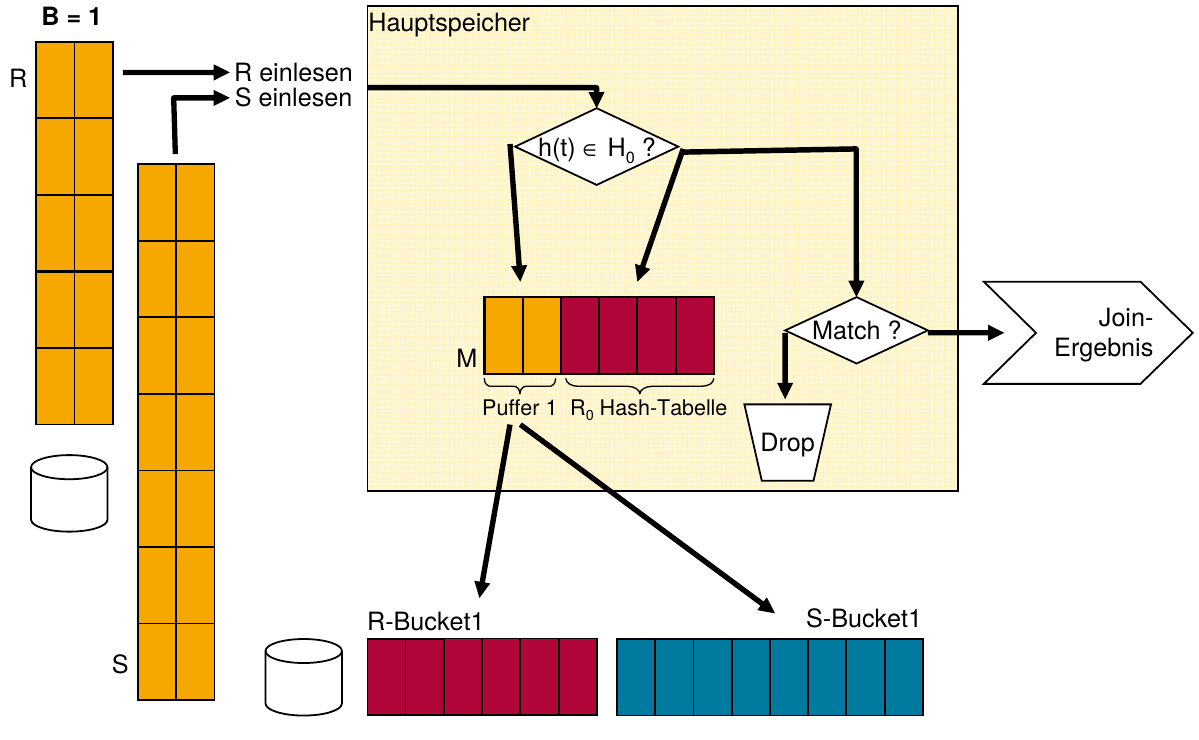
\includegraphics[width=0.4\linewidth]{Bilder/hybrid1.png}}
	\qquad
	\subfloat[][]{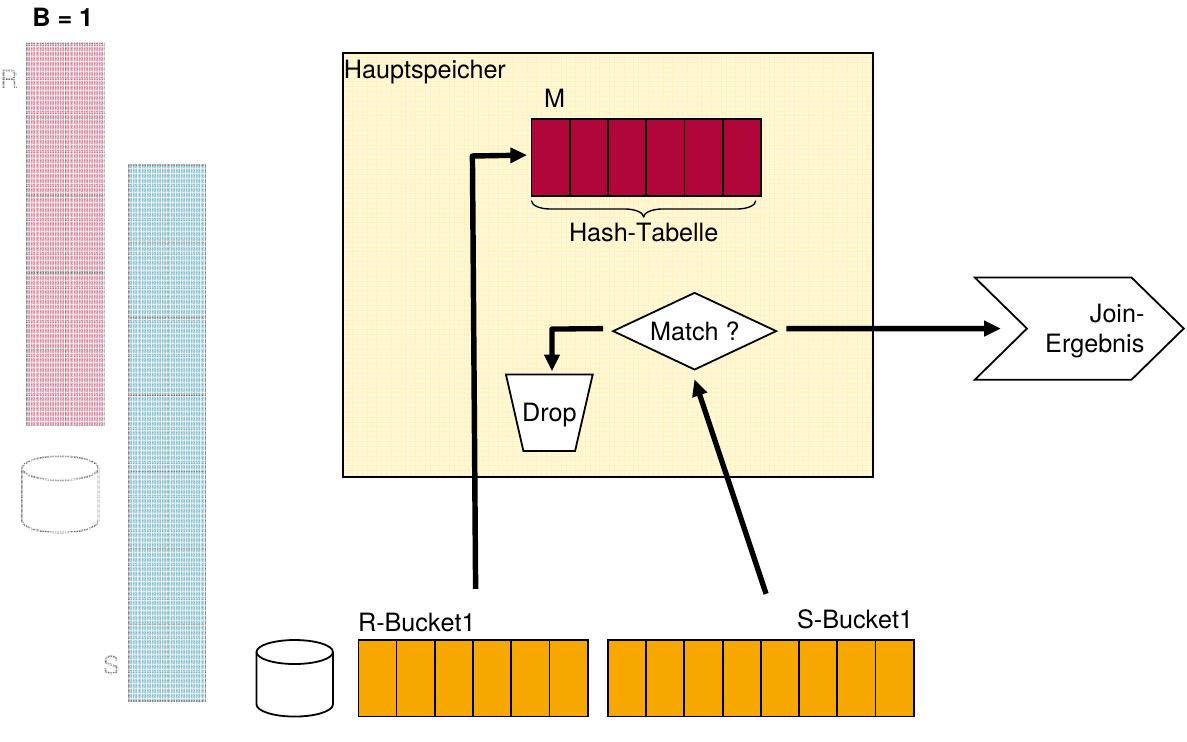
\includegraphics[width=0.4\linewidth]{Bilder/hybrid2.png}}\footnotemark	
	\caption{Hybrid-Hash-Join in 2 Phasen.}
	\label{img:hybrid}
\end{figure}

\footnotetext{\fullcite{Richly2009}}

Anders als der parallele Sort-Operator unterscheidet sich der parallele Hybrid-Hash-Join nur durch eine vorgeschaltete Hash-Partitionierung von der Singlethread-Version. Der Algorithmus, der innerhalb der einzelnen Threads abläuft, ist jeweils ein serieller Hybrid-Hash-Join. In einem ersten Schritt werden also so viele Partitionen erzeugt, wie Kerne für die Worker zur Verfügung stehen, und die entsprechenden Tupel als Strom an die Hash-Join-Worker genannten gleichzeitigen Prozesse verteilt.

Der Algorithmus lässt sich in zwei Phasen aufteilen (siehe \autoref{img:hybrid}). In der ersten Phase wird die erste, also die R-Relation so auf die Buckets verteilt, dass ein Bucket möglichst den dem Thread zur Verfügung stehenden Hauptspeicher vollständig füllt. In diesem Bucket wird eine Hauptspeicher-Hashtabelle angelegt, in der idealerweise in jedem derer Buckets genau ein Tupel gespeichert wird, um die Anzahl notwendiger Vergleiche so gering wie möglich zu halten -- insbesondere wenn durch eine ungünstige Verteilung in der R-Relation oder eine schlechte Hashfunktion sehr viele Tupel in dem gleichen Bucket gespeichert werden, nähert sich der Operator einem Loop-Join an und wird ineffizient. Hier sieht man also bereits, dass die Verteilung vor allem der R-Relation für die Effizienz dieses Algorithmus von großer Bedeutung ist. Die anderen Buckets werden temporär zwischengespeichert, entweder in einer Auslagerungsdatei oder im Hauptspeicher. In einem zweiten Schritt wird die zweite, also die S-Relation gescannt. Tupel, die dem ersten Bucket zugeordnet werden, können direkt in der ersten Phase verschmolzen und an den Ergebnisstrom weitergegeben werden, wenn sie in dem Join-Attribut mit dem Tupel der ersten Relation übereinstimmen. Die anderen Buckets werden wie bei der R-Relation für eine Verarbeitung in der zweiten Phase temporär zwischengespeichert. \autoref{list:hybrid} zeigt den Ablauf der ersten Phasen. Da zum Abschluss der ersten Phase beide Relationen einmal durchlaufen worden sind, können Statistiken ermittelt werden, die es in der zweiten Phase ermöglichen, anstatt mit vorher festgelegten Werten für die Anzahl der Buckets mit einer Abgeschätzung zu arbeiten. Auch wenn dies nicht vollständig verhindern kann, dass einzelne Hashtabellen nicht in den Hauptspeicher passen, ist es doch ein wichtiger Ansatz, um die Chance möglicher Overflows zu reduzieren.   

\begin{minipage}{0.95\textwidth}
	\begin{lstlisting}[caption={Phase 1 Hybrid-Hash-Join.}, label=list:hybrid] 
	lese naechsten Tuple aus R;
	while (Tupel aus R ungleich null) 
		bucket = berechne Bucket mit Hashfunktion;
		if (bucket = 0)
			if (Tupel passt nicht mehr in Speicher)
				speichere Tupel fuer Overflow-Behandlung und merke, ab welchem Bucket es auftritt;
			elseif
				speichere Tupel in interner Hashtabelle;
		elseif
			speichere Tupel in persistenter Hash-Tabelle;
		lese naechsten Tuple aus R;
	endwhile
	
	lese naechsten Tuple aus S;
	while (Tupel aus R ungleich null)
		bucket = berechne Bucket mit Hashfunktion;
		if (bucket = 0)
			if (bucket im Overflow-Bereich von R)
				speichere Tupel fuer Overflow-Behandlung; 
			elseif
				for (alle Tupel im entsprechenden Bucket)
					if (TupelR und TupelS gleich in Joinattribut)
						result = concat(tupleR, tupleS);
						speichere result im Resultbuffer;
					elseif
						loesche TupelS;
		elseif
			speichere Tupel in persistenter Hash-Tabelle;
		lese naechsten Tuple aus S;
	endwhile
	\end{lstlisting}
\end{minipage}

In der zweiten Phase werden dann die restlichen Buckets der ersten Aufteilung der Reihe nach in den Hauptspeicher geladen und in der gleichen Art und Weise Tupel bestimmt, die in ihren Joinattributen übereinstimmen. Da jetzt bereits bekannt ist, ob die einzelnen Buckets in den Hauptspeicher passen, müssen nicht mehr, wie in Phase 1, bei einem Überlauf Teile eines Buckets in eine Überlaufstruktur geschrieben werden, sondern diese kann direkt angelegt werden.

Der Umgang mit möglichen Overflows macht den Algorithmus deutlich komplexer als in einer Version, in der unendlich viel Hauptspeicher zur Verfügung stünde. Auch wenn in vielen Fällen Hash-Join-Algorithmen sehr effizient sind, haben sie jedoch ein schlechtes Worst-Case-Verhalten, da in einem Extremfall alle Tupel den gleichen Hash-Wert hätten. Damit der Algorithmus auch für ungünstig verteilte Relationen funktioniert, wird die Overflow-Behandlung rekursiv angelegt. Die Grundstruktur des Algorithmus bleibt dabei dieselbe, aber in jedem Durchlauf kann erneut ein Overflow auftreten. Da dies das gute Verhalten des Hybrid-Hash-Joins bezüglich der I/O-Kosten umkehrt, ist es sehr wichtig, im ersten Scan einer Relation Statistiken über diese zu generieren, die die Hashfunktion so optimiert, sodass möglichst keine Overflows auftreten.

\subsubsection{Spatial-Join}
\label{entw:spatial}

Aufgrund einer besseren Vergleichbarkeit mit den bereits in \Fb{Secondo} vorhandenen Operatoren habe ich den Spatial-Join auf zwei Operatoren aufgeteilt, nämlich einen Filter-Schritt (\Fb{MThreadSpatialJoin}) \footnote{Die Bezeichnung ist hier etwas verwirrend. Der Filter-Schritt ist nicht der spätere Filter-Operator, sondern der Refinement-Schritt entspricht dem Filter-Operator.} und einen Refinement-Schritt (\Fb{MThreadFilter}), auch wenn ein Performance-Vorteil zu erwarten wäre, wenn beide Operatoren zusammengefasst werden, da einerseits eine Weitergabe des Tuplestroms über die Stream-Schnittstelle des \Fb{Secondo}-Kerns entfallen würde und die Möglichkeit eines dynamischen Load Balancing bestände Ein Vorteil der Trennung ist, dass ein separater Filter-Operator für den Refinement-Schritt universell nutzbar ist.

Um den Operator zu parallelisieren, ist es notwendig, beide Relationen zu partitionieren. Hier bietet sich eine Gitter-Partitionierung an. Um zu vermeiden, dass die Verteilung auf die Gitterzellen sehr ungleichmäßig wird, wähle ich hier ein irreguläres Gitter, welches mit der \Fb{Sort-Tile-Recursiv}-Technik (STR) erzeugt wird. Ein mit STR erzeugtes Gitter stellt sicher, dass die Gitterzellen gleich viele Objekte beinhalten. Um hier den Rechenaufwand zu reduzieren, wird das Gitter nur aus einer Zufallsstichprobe erzeugt, deren Größe mit der Relation wächst. Da dann nicht sichergestellt werden kann, dass alle Objekte im Gitter liegen, ist das Gitter an den Rändern offen. Ein anderer sinnvoller Ansatz der Partitionierung wäre es, über Zweige eines R-Baums zu partitionieren. Der Vorteil wäre, dass der erste Scan der R-Relation während der Partitionierungsphase bereits für den Aufbau der Datenstruktur für den Join-Prozess genutzt werden könnte. Der R-Baum würde dann allerdings nicht parallel erzeugt werden. Ich habe mich gegen einen globalen R-Baum entschieden, um einerseits auch die Baum-Erzeugung parallelisieren zu können und da andererseits die Eliminierung von Duplikaten in einer Gitterstruktur nicht rechenaufwändig ist. Hinzu kommt, dass der interne R-Baum von \Fb{Secondo} bisher keine Methode enthält, um auf Teilbäume zuzugreifen -- aber diese zu implementieren, wäre nicht aufwändig.

Das Scheduling des Filterschritts konstruiert für die Partitionierung ein \Fb{SRT}-Gitter, erzeugt die Worker-Threads, partitioniert die beiden Relationen $R$ und $S$ für die entsprechenden Worker-Threads und sammelt abschließend den Ergebnisstrom ein und gibt ihn an den Strom für den folgenden Operator weiter. Also entspricht auch dieser Operator einem Master-Worker-Schema. Es hat sich als wesentlich effizienter erwiesen, nicht nur für jeden genutzten Kern einen Thread zu erzeugen, sondern in ein Gitter mit der Anzahl von Kernen als Kantenlänge zu partitionieren (also das Quadrat der parametrisierten Kernzahl an Threads zu verwenden). Dementsprechend werden meist mehr Threads verwendet als Kerne im System zur Verfügung stehen, die aber teils wegen Hyperthreading noch parallel ausgeführt werden können.

\begin{figure}
	\centering
	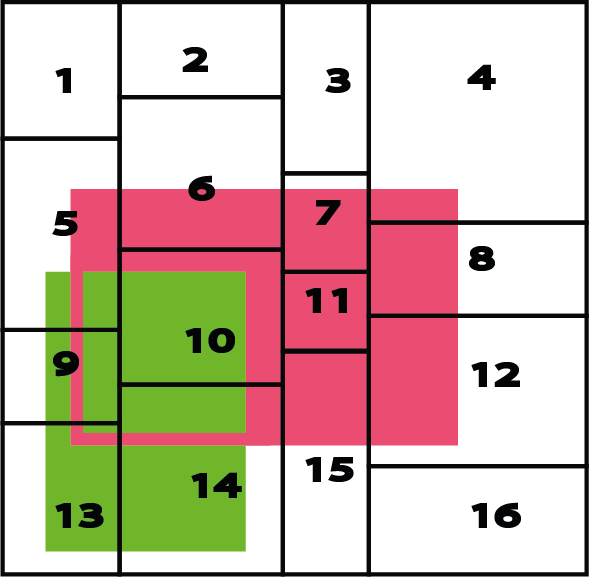
\includegraphics[width=0.4\linewidth]{Bilder/duplikat.png}
	\caption{Erkennung von Duplikaten im Spatial-Join.}
	\label{img:sjDup}
\end{figure}

Hier soll ein Spatial-Join-Operator implementiert werden, der keine spezifischen Voraussetzungen hat. Es wird davon ausgegangen, dass weder Indices noch Statistiken über die Relationen vorliegen. Also kommen vor allem zwei Algorithmen infrage: der Spatial-Hash-Join oder ein iterativer Spatial-Join mit einem R-Baum. Auch wenn in der Literatur für den hier vorliegenden Kontext häufig Spatial-Hash-Joins empfohlen werden, haben diese zwei Nachteile. Bei unbekannten Relationen ist es schwer, ein optimales Gitter zu bestimmen. Gibt es zu viele Gitterzellen, werden viele Duplikate erzeugt, die auch jedes Mal erneut auf die Joinbedingung getestet werden müssen;  gibt es zu wenig Gitterzellen, liegen viele Objekte in der gleichen Gitterzelle. Verschärft wird das Problem noch dadurch, dass ein Spatial-Hash-Join sehr anfällig gegenüber einer ungünstigen Verteilung in den Relationen ist. Die Verwendung eines Gitters wie es für die Partitionierung verwendet wird, wäre zwar eine Lösung für den Umgang mit unterschiedlichen Verteilungen, die aber wesentlich zu teuer wäre. Deswegen entscheide ich mich hier, einen internen R-Baum zu erzeugen und die zweite Relation seriell zu durchlaufen. Für den Fall, dass die Relation, über die ein R-Baum erzeugt wird, nicht in den Hauptspeicher passt, muss dieser Prozess mehrfach wiederholt werden. Deswegen wird von einem iterativen Spatial-R-Baum-Join gesprochen.

Anders als bei den beiden anderen implementierten Operatoren ist es nicht nur eine Frage der Performance, ob der Algorithmus gegenüber einer Singlethread-Variante modifiziert wird. Ein prinzipieller Unterschied einer parallelen Implementierung ist, dass räumliche Objekte, sofern sie eine Ausdehnung haben, mehreren Gitterzellen und damit Partitionen gleichzeitig zugewiesen werden können (siehe Mehrfachzuweisungs-Single-Joins in \autoref{Spatial Join}). Dementsprechend können im Filter-Schritt gleiche Joinkandidaten in unterschiedlichen Threads und damit doppelt ermittelt werden. Im Anschluss an den Join Duplikate als zusätzlichen Schritt zu eliminieren, ist sehr rechenaufwändig. Wird lediglich der Kandidat weitergegeben, dessen Schnittmenge der räumlichen Joinattributs aus der Relation R und S in der Gitterzelle liegt, die sich so weit wie möglich rechts und oben befindet, werden Duplikate bereits in der Entstehung ausgeschlossen. Im Beispiel in \autoref{img:sjDup} schneiden sich zwei \Fb{MBBs} und werden als Joinkanditat in den Gitterzellen 5, 9, 10, 13 und 14 erkannt. Weitergegeben wird aber nur der Treffer, der in Gitterzelle 10 festgestellt worden ist.

In den Worker-Threads werden zuerst die Tupelströme aus den Partitionen der R-Relation in einen internen R-Baum eingelesen. Jedem Thread wird ein gleicher Teil des Hauptspeichers zur Verfügung gestellt. Tupel, die nicht mehr in den Hauptspeicher passen, werden ausgelagert. In einem ersten Schritt wird die S-Relation einmal gescannt, Joinkandidaten bestimmt und diese auf Duplikate geprüft. Sofern es einen Overflow gab, kann die Anzahl der notwendigen Iterationen jetzt genau berechnet werden, da die Größe der R-Relation bereits bekannt ist. In jeder Iteration wird die S-Relation wiederum vollständig durchlaufen und für einen weiteren disjunkten Teil der R-Relation ein Hauptspeicher-R-Baum aufgebaut.

\begin{minipage}{0.95\textwidth}
	\begin{lstlisting}[caption={Spatial-Join: Worker.}, label=list:spatialJoin]
	tupleR = lese aus Buffer R;
	freeMem = Speicher, der dem Thread zugewiesen wurde; 
	while (tupleR != nullptr)
		if (freeMem > 0)
			speichere tupleR in R-Baum mit MBB;
			berechne freeMem neu aus Tupel und R-Baum;
		elseif
			speichere tupleR in Overflow;
		tupleR = lese aus Buffer R 
	endwhile
	tupleS = lese aus Buffer S
	while (tupleS != nullptr)
		ueberpruefe, ob MBB von tupleS Objekte im R-Baum schneidet;
		for (alle Ergebnisse)
			if (kein Duplikat)
				result = concat(tupleR, tupleS);
				speichere result im Resultbuffer;
		tupleS = lese aus Buffer R
	endwhile
	\end{lstlisting}
\end{minipage}

Auch wenn hier ein sehr großer Performance-Vorteil zu erwarten ist, da die Berechnungen räumlicher Beziehungen bei komplexen räumlichen Objekten sehr rechenintensiv ist, ist die Grundidee des Filter-Operators sehr einfach. Anstatt einen genau auf die Bedürfnisse zugeschnittenen Operator für das Refinement zu implementieren, habe ich mich hier entschieden, einen allgemeinen, universell einsetzbaren Filteroperator für diesen zweiten Schritt des Spatial-Joins einzusetzen. Der Tupelstrom wird nach Round Robin auf die einzelnen Threads verteilt, die nur die Tupel zurückgeben, die das Filterprädikat erfüllen. Die Berechnung der Prädikate übernimmt der Query-Prozessor.

\subsection{Implementierung}
\label{Implemeniterung} 

Im folgenden wird die Implementierung der in \autoref{Entwicklung} skizzierten Operatoren und der Datenstrukturen, die von den Operatoren gemeinsam genutzt werden, dargestellt. Einleitend werde ich einerseits die genutzte Entwicklungsumgebung skizzieren und andererseits wichtige Ansätze in der Implementierung erläutern, die von übergreifender Bedeutung sind.

Die von mir implementierte Algebra habe ich in einem \Fb{OpenSuse~Leap~15.0} Linux-System in \Fb{Secondo} 4.20 integriert. Als IDE wurde \Fb{C-Lion} verwendet. Für meine Implementierung musste ich ausschließlich eine Algebra im \Fb{Secondo}-Kern in\Fb{C++} integrieren und einige Änderungen im Kern und in anderen Algebren vornehmen. Genutzt wurde der\Fb{C++11}-Standard. Vor allem habe ich die ab diesem Standard neu in die Standard-Library integrierte Concurrency-Bibliothek und \Fb{shared\_pointer} verwendet.

Mit\Fb{C++11} wurde die Concurrency-Implementierung der \Fb{Boost}-Library in die Standardbibliothek übernommen, die ich in meiner Implementierung verwende. Sie basiert auf dem\Fb{C++}-Speichermodell, der sequentiellen Konsistenz. Es muss also ein deterministisches Verhalten auch eines Programmflusses garantiert werden, der auf mehreren gleichzeitigen Prozessen beruht. Kern der\Fb{C++}-Concurrency-Schnittstelle sind Threads, die ihre ausführbare Einheit enthalten und sofort gestartet werden. Ich verwenden durchgehend Funktionsobjekte, das heißt Instanzen von Klassen, für die der Klammer-Operator überladen worden ist. Der erzeugende Thread kann entweder mit \Fb{join} darauf warten, dass der Thread seine Aufgaben beendet oder den Thread mit \Fb{detach} vom Erzeuger-Thread lösen, mit dem Risiko von undefiniertem Verhalten, da die Existenz gemeinsame genutzer Resssourcen so nicht mehr garantiert ist. Sperren können in Mutexe verpackt werden, von denen ich zwei mit unterschiedlichen Kosten und Funktionsumfang verwende: den \Fb{lock\_guard}, der lediglich sicherstellt, dass die Sperren wieder freigegeben werden und den \Fb{unique\_lock} mit erweiterter Funktionalität. Für meine Implementierung wichtig ist seine Möglichkeit, die Sperre pausieren zu lassen, also Sperren mehrfach zu setzen und wieder freizugeben. Mithilfe von Bedingungsvariablen (\Fb{condition\_variable}) kann auf einer Nachricht an einen oder alle Threads gewartet werden. Anzuraten ist es, um Nebeneffekte zu vermeiden, ein Prädikat in Form einer Lambda-Funktion zu verwenden. \Fb{Std::atomic} stellt darüber hinaus atomare Datentypen zur Verfügung, von denen ich atomare Booleans verwende \parencite{Grimm2018}. 

\begin{minipage}{0.95\textwidth}
	\begin{lstlisting}[caption={Flags der \Fb{MThreaded}-Algebra.}, label=list:flags]
	DEFAULTCCFLAGS += -pthread -DTHREAD_SAFE
	CCFLAGS += -pthread -DTHREAD_SAFE
	COMMON_LD_FLAGS += -lboost_thread -lboost_system
	\end{lstlisting}
\end{minipage}

Eine Schwierigkeit meiner Implementierung ist es, dass ich zwar in der von mir entworfenen Algebra die sequentielle Konsistenz garantieren kann, aber diese an diversen Stellen auf anderen Funktionalitäten des \Fb{Secondo}-Kerns beruht. Probleme traten vor allem im Umgang mit \Fb{FLOBs} auf, aber auch teils mit Standardtypen, wenn im Operatorenbaum dem parallelen Operator folgend nur sehr wenige aufwändige Operatoren folgten \footnote{So stürzt der Hash-Join beispielsweise ohne auch mit Standard-Datentapen ab, wenn ihm nur ein \Fb{count} folgte, aber nicht, wenn alle Ergebnisse mit \Fb{consume} an die Console ausgegeben wurden.}. Die Probleme äußerten sich selten in dem von mir implementierten Operator (gelegentlich in Aufrufen des Flob-Managers), sondern vor allem darin, dass Zähler für Datenbanktabellenzeiger entweder in den Folgeoperatoren korrupt wurden oder meist in Abstürzen durch falsche Zeiger auf Datenbankstrukturen, korrupte Sperren oder Deadlocks im Commit. 

\Fb{Secondo} verwendet die Berkeley-DB in einer Konfiguration, die keinen konkurrierenden Zugriff auf die Datenbankschicht durch den Storage-Mangager erlaubt. Deswegen muss sichergestellt werden, dass Zugriffe auf diese nur sequentiell stattfinden. Im Standard-\Fb{Secondo} gab es Probleme mit der Thread-Sicherheit des Flob-Managers bzw. allgemein bei der Verwendung von \Fb{FLOBs}. Über ein Flag lässt sich \Fb{Secondo} in einem Thread-sicheren Modus kompilieren (siehe \autoref{list:flags}). Vor allem wird bei Verwendung dieses Flags der Flob-Manager synchronisiert, aber auch die Relational-Algebra und Teile des Storage-Managers. Leider gab es in der von mir implementieren Algebra weiterhin Probleme mit der Threadsicherheit, sofern direkt auf \Fb{FLOBs} innerhalb von Threads zugegriffen wird. Vor allem tritt dieses Problem bei der Verwendung von Query-Prozessoren innerhalb der Threads im Filter-Operator auf und sofern Attribute in den beiden anderen Operatoren \Fb{FLOBs} sind. Im Detail werde ich das Problem und geeignete Lösungsversuche im \autoref{impl:refinement} diskutieren. Ein Problem bei der Implementierung ist, dass nicht immer einfach entschieden werden konnte, ob Probleme mit der Stabilität eines Operators an Mängeln der Synchronisation beim Zugriff auf \Fb{FLOBs} liegen oder an Fehlern in meiner Implementierung.

Abhängigkeiten bestehen zu folgenden Algebren, die mithilfe des Makefiles der Algebra eingebunden werden:

\begin{itemize}
	\item \Fb{StandardAlgebra}
	\item \Fb{StreamAlgebra}
	\item \Fb{RelationAlgebra}
	\item \Fb{SpatialAlgebra}
	\item \Fb{RectangleAlgebra}
	\item \Fb{SPartAlgebra} (irreguläres Gitter)
\end{itemize}

Die Schnittstelle für die Integration neuer Operatoren ist genau definiert. Prinzipiell besteht ein Operator aus vier Methoden und zwei zusätzlichen Dateien: Das Type-Mapping stellt sicher, dass ein Operator nur mit Parametern aufgerufen wird, mit denen er funktioniert. Das Value-Mapping berechnet aus einer Eingabe das Ergebnis. Die Methode \Fb{getOperatorSec} enthält die Spezifikation des Operators als Text. Die Methode \Fb{getOperator} fasst die Bestandteile des Operators für den Algebra-Manager zusammen. Zusätzlich notwendig ist eine Datei mit mindestens einem Beispiel für jeden Operator, mit der das Funktionieren der Algebren automatisch überprüft werden kann, und eine Datei, die die Signatur der Operatoren enthält. Alle von mir implementierten Operatoren außer den Operatoren für die Parametrisierung, auf die ich hier nicht genauer eingehe, da sie sehr simpel aufgebaut sind, haben als Eingangs- und Ergebniswert einen Tupelstrom. Hier ist es notwendig, den Zustand des Operators in einer weiteren Klasse zu erhalten, die \Fb{LocalInfo}-Klasse genannt wird. In meiner Implementierung übernimmt sie auch die Funktion des Schedulings, also verteilt Daten, gibt das Ergebnis weiter und erzeugt sowie verwaltet die notwendigen Datenstrukturen und Threads. Zwei Parameter werden für einige Operatoren gesetzt. \Fb{SetUsesMemory} erlaubt es einem Operator, seinen Speicher selbst zu verwalten und ist notwendig bei Operatoren, die größere Datenstrukturen im Hauptspeicher aufbauen. \Fb{SetUsesArgsInTypeMapping} erlaubt im Type-Mapping den Zugriff auf die Parameter. Ein wichtiger Mechanismus des Type-Mappings, der hier genutzt wird, ist der Append-Mechanismus, der die Weitergabe von dort generierten Informationen an das Value-Mapping erlaubt.

Grundsätzlich verwende ich Headerdateien, damit die Schnittstellen einfacher erfasst werden können. Die Implementierungen der Operatoren sind in Ordnern zusammengefasst nach Hilfsoperatoren für die Parametrisierung, Sortieroperatoren (mit dem Sort-Operator) und Join-Operatoren(mit dem Hash-Join, dem Spatial-Join und dem Filter-Operator). Hilfsstrukturen, die von mehreren Operatoren genutzt werden und darüber hinaus für weitere Algebren zur Verfügung gestellt werden sollen, sind in \Fb{MThreadedAux} zusammengefasst. Weitere Tests, die in \autoref{te} verwendet werden, sind im Ordner \Fb{test-specs} zusammengefasst.

\subsubsection{Hilfsstrukturen}
\label{Hilfsstrukturen} 

In diesem Kapitel stelle ich selbst implementierte Datenstrukturen vor, die nicht speziell einem Operator zugeordnet werden können, sondern von mehreren Operatoren genutzt werden. Die Operatoren-übergreifend genutzten Datenstrukturen sind in der Datei \Fb{methreatedAux} zusammengefasst. Ich habe drei unterschiedliche Tupelbuffer implementiert und zwei threadsichere Wrapperklassen um die Warteschlange der Standard-Library. Unterschiede zwischen den verschiedenen Versionen ist die Fähigkeit, Tupel zwischenzuspeichern.

Tupelbuffer sind für Anwendungsfälle gedacht, bei denen der Schreib- und der Lesevorgang voneinander zeitlich getrennt ist -- im Allgemeinen wird zuerst eine bestimmte Menge von Tupeln temporär gespeichert, um später wieder vollständig geladen zu werden. Da bei der Initialisierung oft nicht klar ist, ob der Buffer im Hauptspeicher gehalten werden kann oder nicht, habe ich eine virtuelle Klasse für Buffer implementiert, von der Versionen mit gleicher Schnittstelle abgeleitet sind: ein Hauptspeicherbuffer, ein persistenter Buffer und ein Buffer, der intern verwaltet, ob er im Hauptspeicher gehalten werden kann. Intern verwenden die Tupelbuffer, sofern es sich um die Hauptspeicherversionen handelt, als Datenstruktur Warteschlangen und sofern es sich um persistente Buffer handelt, einen Zeiger auf \Fb{TupleFiles} der \Fb{RelationAlgebra}. Im persistenten Fall wird dessen \Fb{MakeScan}-Iterator für den Zugriff auf die Daten verwendet. Zuerst habe ich die temporären Speicher selbst mit \Fb{fileStreams} und der Methode \Fb{WriteToBin} der Tupel-Klasse implementiert, aber mit diesem Ansatz gab es, sofern \Fb{FLOBs} verwendet wurden, Synchronisierungsprobleme. Die Buffer haben eine Read-, eine Append-Methode, Methoden zum Öffnen sowie Schließen und zur Abfrage, ob der Buffer leer ist. Die Hauptspeicherversion des Buffers verfügt über einige Methoden über keinen Code, die aber notwendig waren, damit alle Versionen mit einem gleichen Interface benutzt werden können. Sowohl die persistenten Buffer als auch die Warteschlangen wurden so konstruiert, dass Dateien nicht direkt im Konstruktor angelegt werden, sondern erst, wenn der erste Schreibvorgang notwendig wurde, um zu verhindern, dass I/O-Operationen durch die Anlage einer Datei notwendig werden, sofern keine Persistierung erfolgen, aber der Buffer bereits erzeugt werden musste.

\begin{minipage}{0.95\textwidth}
	\begin{lstlisting}[caption={Enqueue und Dequeue-Methode der threadsichere Warteschlange.}, label=list:queue]
	void enqueue(T t) {
		std::lock_guard<std::mutex> lock(m);
		q.push(t);
		dataReadyQueue = true;
		c.notify_one();
	}
	T dequeue() {
		std::unique_lock<std::mutex> lock(m);
		while (q.empty()) {
			c.wait(lock, [&] { return dataReadyQueue; });
			dataReadyQueue = false;
		}
		T val = q.front();
		q.pop();
		return val;
	}
	\end{lstlisting}
\end{minipage}

Die Warteschlange der Standard-Library ist nicht threadsicher. Verwendung finden Warteschlangen vor allem als Buffer für den Datenaustausch zwischen Threads, zwischen denen Tupelströme fließen. Eine persistente Version wurde notwendig, da die Join-Operatoren teils blockieren und bereits deutlich früher einen Ergebnisstrom produzieren als begonnen wird diesen auszulesen. Deswegen kann es vorkommen, dass bei einem Join umfangreicher Relationen mit einer großen Ergebnismenge die Buffer nicht mehr in den Hauptspeicher passen. Die nicht persistente Version ist generisch angelegt und damit nicht nur für Tupel nutzbar. Für die Synchronisierung wird ein Mutex verwendet. Die \Fb{Dequeue}-Methode gibt diesen temporär wieder frei, wenn die Warteschlange leer ist, um in diesem Fall einen Schreibvorgang zu ermöglichen (\autoref{list:queue}). Die persistente Version wird mit dem zur Verfügung stehenden Hauptspeicher parametrisiert und lagert ab dem Zeitpunkt, an dem kein Speicher mehr zur Verfügung steht, die Tupel in ein Fb{TupleFile} aus. Eine Verbesserungsmöglichkeit wäre es, wenn anschließend wieder Hauptspeicher frei werden würde, diesen auch zu verwenden, was in der derzeitigen Implementierung nicht der Fall ist.

\subsubsection{Operatoren für die Parametrisierung}

Die Operatoren für die Parametrisierung haben folgende Signaturen:

\begin{itemize}
	\item maxcore: $\longrightarrow int$
	\item setcore: $int \longrightarrow bool$
	\item getcore: $\longrightarrow int$
\end{itemize}

Die Anzahl der genutzten Kerne wird in einem Singleton in einer statischen Variablen gespeichert. Die Anzahl der maximal nutzbaren Kerne wird über eine Methode der Concurrency-Library ermittelt.

\subsubsection{2-Wege-Merge-Sort}

Der Operator \Fb{mThreadedMergeSort} hat die Signatur: \newline
$stream~x~(attr~x~bool \ldots) \longrightarrow stream$
 
In die Algebra muss er mit zwei Optionen integriert werden: Er muss seinen Speicher selbst verwalten, um zu wissen, wie viel Arbeitsspeicher für die Sortierung der Läufe zur Verfügung steht, und er benötigt seine Argumente im Type-Mapping, um die Sortierrichtung auswerten und weitergeben zu können. Das Type-Mapping hat zwei Funktionen: Einerseits muss es sicherstellen, dass die zu sortierende Relation als Tupelstrom in den Operator eingeht und die Sortierattribute Elemente der Tupel sind. Andererseits wird der Append-Mechanismus genutzt, um die Indices der Sortierattribute und die Sortierrichtung an das Value-Mapping weiterzugeben. Die Attribute und die Sortierrichtung werden dem Operator als Liste übergeben, um zu ermöglichen, dass beliebig viele Sortierattribute genutzt werden können, wobei die Richtung als Boolean übergeben werden kann. Wenn keine Richtung explizit gewählt ist, wird sie als aufsteigend gesetzt. Der Operator bricht nur ab, wenn keines der Attribute in der Relation vorkommt; in den anderen Fällen werden lediglich falsche Attribute ignoriert. 

\begin{figure}
	\centering
	\includegraphics[width=0.75\textwidth]{Bilder/mergeSort.png}
	\caption{Aufbau des Mergesort-Operators (vereinfacht). Gestrichelte Pfeile: Datenfluss; durchgezogene: Instanzen werden erzeugt.}
	\label{img:KlassSort}
\end{figure}

Alle verwendeten Klassen und ihre Beziehungen zeigt \autoref{img:KlassSort}. Das Value-Mapping startet lediglich die \Fb{LocalInfo}-Klasse mit den Suchindices sowie dem verfügbarem Arbeitsspeicher als Argument und holt den sortierten Tupelstrom aus der Pipeline-Instanz, die die Wurzel des Merge-Baumsstruktur darstellt, über dessen \Fb{GetNext}-Methode ab. Die \Fb{LocalInfo}-Klasse ist verantwortlich für das Scheduling, Destributor-Collector genannt, das heißt, für die Erzeugung der notwendigen Buffer, der Threads und das Verteilen des eingehenden Stroms auf die Threads. Als Buffer für die Läufe werden die in \autoref{Hilfsstrukturen} dargestellten, selbst implementierten Klassen verwendet, die Daten sowohl im Speicher halten, als auch in eine temporäre Datei auslagern können. Für den Tupelstrom innerhalb der Merge-Pipeline und für die vollständig sortierte Relation wird eine Wrapper-Klasse um die Warteschlange der Standardbibliothek benutzt, die threadsicher gemacht wurde. Vergleiche werden über eine Compare-Klasse vorgenommen, die mit dem Sortiervektor initialisiert wird.

Die Partitionierung weißt abwechselnd allen Workern einen Tupel aus dem Strom zu. Zuerst habe ich die Weitergabe über Iteratoren organisiert. Da der Worker jedes mitteilen musste, wenn er ein Tupel entnommen hat, war ein hoher Synchronisationsaufwand mit Mutexen und Nachrichten über Bedingungsvariablen notwendig. Eine Weitergabe der Tupel über die von mir implementierte threadsichere Warteschlange brachte einen Performancegewinn von ca. 50~\% -- dies zeigt die Kosten, die durch aufwändige Synchronisierung verursacht werden können.

Anschließend wird aus den Elementen Merge-Feeder, NoMerge-Feeder und Merge-Pipeline die Merge-Pipeline erzeugt. Die Threads werden vom Hauptthread entkoppelt, um einen nicht-blockierenden Operator zu ermöglichen, also nach dem Start der Merge-Pipeline sofort die ausgegebenen Tupel über die \Fb{GetNext}-Methode abholen zu können. Im Gegensatz dazu hat es zu undefiniertem Verhalten geführt, auch in der suboptimalen Phase die Threads zu entkoppeln. Der Vorteil einer Entkopplung wäre es, dass, sofern einige Threads der suboptimalen Phase deutlich schneller sind als andere zum Beispiel aufgrund einer teilweisen Vorsortierung, bereits frühzeitig Teile der Merge-Pipeline hätten gestartet werden können. So lässt sich die Laufzeit der unterschiedlichen Äste der Merge-Pipeline nur noch darüber regulieren, dass die Läufe, die im Hauptspeicher gehalten werden konnten, in die aufwändigeren \Fb{MergeFeeder} eingehen.

Wie bereits in \autoref{Entwicklung} dargelegt, läuft die suboptimale Phase in zwei Schritten ab, nämlich der Erzeugung von sortierten Läufen und der Reduktion der Läufe auf genau einen durch mehrere Merge-Phasen. Der erste Schritt wiederum ist in drei Phasen aufgeteilt: Als internes Sortierverfahren wird ein Heap-Sort mit einem Wettbewerbsbaum als Datenstruktur (siehe unten) verwendet. In der ersten Phase werden die Blätter des Wettlaufbaums gefüllt und kontinuierlich überwacht, ob noch genügend Speicher vorhanden ist. Der Arbeitsspeicher wird gleichmäßig zwischen den Threads aufgeteilt. Ein Abbruchkriterium für das Füllen des Baums ist, wenn der Speicher durch einen vollständig konstruierten Baum sowie die Speicherrepräsentation der Tupel ausgelastet ist. Im Baum selbst werden nur Pointer auf Tupel gespeichert. Ein zweites Abbruchkriterium ist, wenn der Tupelstrom erschöpft ist, gekennzeichnet durch die Weitergabe eines Nullpointers. Dem folgend wird der vollständige Baum von den Blättern ausgehend konstruiert.

Die Läufe werden in selbst implementierten Tupelbuffern gespeichert, die entweder speicherintern sind oder in eine Datei ausgelagert werden können (vgl. \autoref{Hilfsstrukturen}). Weitere Läufe zu erzeugen ist nur notwendig, wenn der Tupelstrom nach der Füllung des ersten Baums noch nicht erschöpft ist, da im anderen Fall bereits genau ein sortierter Lauf erzeugt worden ist, der auch nicht persistiert werden muss. Diese weiteren Läufe werden dadurch erzeugt, dass das aktuelle Tupel des Eingangsstroms mit der Wurzel des Baums ausgetauscht wird und dieser neue Wert weiter in den Baum einsickert. Aus den ausgetauschten Tupeln werden die weiteren Läufe erzeugt, die immer in persistenten Buffern gespeichert werden. Ein neuer Lauf wird angelegt, wenn der aktuelle Wert nicht mehr in den Baum einsickern kann, das heißt, wenn die Wurzel inaktiv ist (die genaue Funktionsweise des Heap-Sorts mithilfe eines Wettbewerbsbaums werde ich im nächsten Abschnitt erläutern). Abschließend werden zuerst alle aktiven Knoten in den aktuellen Lauf und dann der restliche Baum in einen neuen Lauf gelesen, indem die Tupel im Baum durch Nullpointer getauscht werden. Der letzte Lauf kann in einen internen Tupelbuffer geschrieben werden.

\begin{figure}
	\centering
	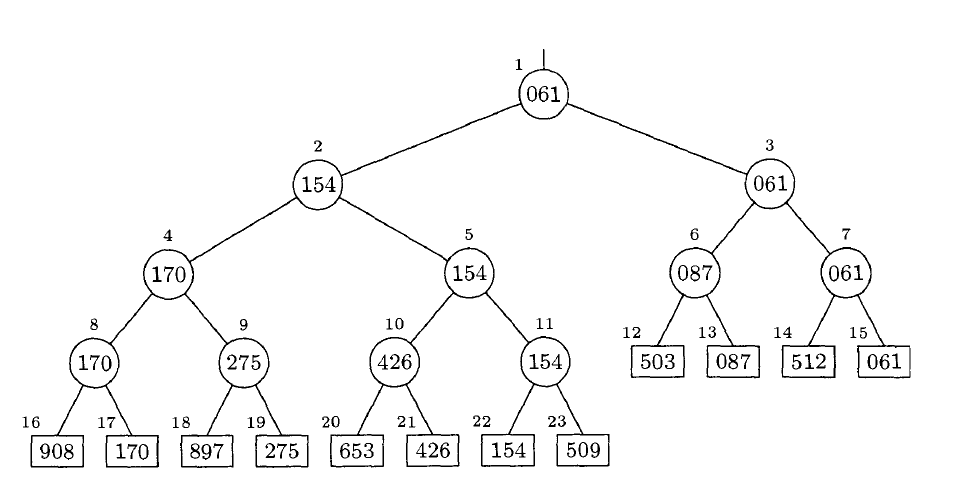
\includegraphics[width=0.75\textwidth]{Bilder/tournament.png}
	\caption{Wettbewerbsbaum \parencite[S. 253]{Knuth1973}.}
	\label{img:tournament}
\end{figure}

Der Wettbewerbsbaum ist eine Datenstruktur, die eine Sortierung vergleichbar mit der Darstellung des Verlaufs eines Tennisturniers abbildet (vgl. \autoref{img:tournament}). Das Sieger-Tupel befindet sich in der Wurzel, in den Kindern jeweils der Sieger-Tupel und ein Tupel mit einem größerem Sortierattribut -- diese Struktur setzt sich weiter fort, bis in den Blättern alle Tupel, die im Baum gespeichert sind, abgebildet sind. In jedem Knoten ist je der Nachfolgeknoten mit dem kleineren und größeren Wert durch den Vektorindex, ein Schalter aktiv/inaktiv und ein Zeiger auf den Tupel gespeichert. Blätter sind dadurch gekennzeichnet, dass als Nachfolgeknoten der größte mögliche vorzeichenlose Integer-Wert eingetragen wird. Als inaktiv werden Tupel gekennzeichnet, die erst in der Erzeugung des nächsten Laufs verwendet werden, da sie für den aktuellen Sortierlauf je nach Sortierrichtung zu groß oder zu klein sind. Ein Baum kann keine weiteren Tupel mehr aufnehmen, wenn die Wurzel inaktiv geworden ist. Wenn der Baum noch Werte im aktuellen Lauf aufnehmen kann, wandern Tupel mithilfe einer rekursiven Methode von der Wurzel zu den Blättern und strukturieren den Baum dabei um. Für einen neuen Lauf muss der Baum lediglich wieder vollständig auf aktiv gesetzt werden. 

Der Merge-Schritt entspricht der in \autoref{entw:sort} beschriebenen Vorgehensweise. In einer Schleife werden je zwei Läufe miteinander zu einem Ergebnislauf verschnitten, bis nur noch ein Lauf übrigbleibt -- verschneiden meint, dass in einer Schleife von zwei Tupeln immer der mit dem kleineren/größeren Wert im Sortierattributs an den Ergebnislauf weitergegeben und anschließend aus dem entsprechenden Eingangslauf ersetzt wird. In der postoptimalen Phase laufen die Verschneidungen vom Prinzip her genauso ab, aber es wird mit einem Tupelstrom gearbeitet, der durch eine Merge-Pipeline fließt, um die zur Verfügung stehenden Kerne optimal ausnutzen zu können. \Fb{Feeder} haben als Eingang die in der suboptimalen Phase erzeugten Läufe und geben sie entweder einfach weiter (\Fb{NoMergeFeeder}) oder verschmelzen sie vorher (\Fb{MergeFeeder}). Diese Unterscheidung ist notwendig, wenn der Baum der Merge-Pipeline kein vollständig gefüllter Baum ist. Der Pipeline-Schritt, der die Wurzel darstellt, gibt seine Ausgabe an den Buffer aus, der von der \Fb{\Fb{GetNext}}-Methode der \Fb{\Fb{LocalInfo}}-Klasse eingelesen wird. In der Pipeline werden Buffer verwendet anstatt lediglich Tupel weitergegeben, um sicherzustellen, dass es nicht zu einer Blockierung kommt, wenn Verarbeitungsgeschwindigkeiten auf unterschiedlichen Ästen verschieden sind. Die Buffer sind \Fb{shared\_pointer} auf die selbst implementierte threadsichere Warteschlange.  


\subsubsection{Hybrid-Hash-Join}
\label{impl:hybrid}

Der Operator \Fb{mThreadedMergeSort} hat folgende Signatur: \newline
$stream~x~(attr~x~bool \ldots) \longrightarrow stream$

In die Algebra muss er mit einer Option integriert werden: Er muss seinen Speicher selbst verwalten, um zu wissen, wie viel Hauptspeicher für die Hashtabellen zur Verfügung steht. Das Type-Mapping hat zwei Funktionen. Einerseits muss es sicherstellen, dass die beiden Relationen, die über einen Equi-Join verbunden werden sollen, als Tupelstrom in den Operator eingehen und die Joinattribute Elemente der jeweiligen Tupel sind. Andererseits wird der Append-Mechanismus genutzt, um die Indices der Joinattribute an das Value-Mapping weiterzugeben.

Auch hier wird das Entwurfsmuster gewählt, welches in \Fb{Secondo} für Operatoren verwendet wird, die einen Tupelstrom als Ein- und Ausgabe haben. \autoref{img:KlassJoin} gibt eine Übersicht über das Klassendiagramm des Operators. Der Zustand des Operators wird in einer \Fb{LocalInfo}-Cass gesichert, auch wenn ein kontinuierlicher Tupelstrom fließt. Diese Klasse hat noch die zusätzliche Aufgabe, innerhalb eines Master-Worker-Schemas die Funktion des Masters zu übernehmen: Sie erzeugt die Worker-Threads, partitioniert und verteilt die Daten über eine Modulo-Hashfunktion auf genau so viele Threads wie Kerne genutzt werden und sammelt den Ergebnis-Tupelstrom abschließend wieder über ihre \Fb{GetNext}-Methode ein. Als Buffer für den die Eingangsströme in die Threads wird ein Vektor mit Shared-Pointen auf eine von mir implementierte threadsichere Queue verwendet. Für jeden Thread existieren genau zwei Buffer für je die R- und S-Relation, auf die die beiden eingehenden Relationen mit einer Modulo-Hashfunktion verteilt werden. Die Threads vom Hauptthread zu entkoppeln, führte zu undefiniertem verhalten. Dies wirkt sich negativ auf die Performance aus, da der Operator blockiert und es vorkommen kann, dass die Ergebnis in eine Datei ausgelagert werden müssen. Mit der Weitergabe der Ergebnis-Tupel durch die \Fb{GetNext}-Methode kann erst begonnen werden, wenn die Berechnung des Joins in den Workern abgeschlossen ist. 

\begin{figure}
	\centering
	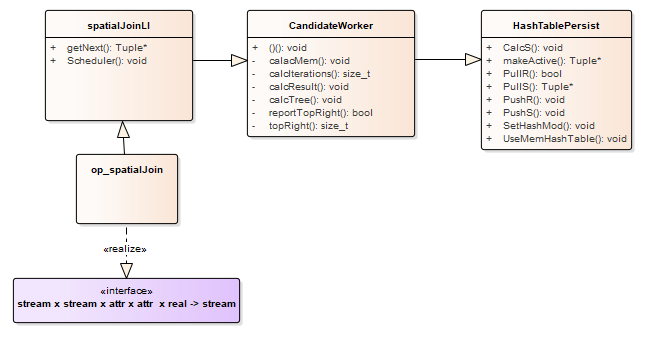
\includegraphics[width=0.75\textwidth]{Bilder/hybridJoin.png}
	\caption{Aufbau des Hybrid-Hash-Join-Operators (vereinfacht). Gestrichelte Pfeile: Datenfluss; durchgezogene: Instanzen werden erzeugt.}
	\label{img:KlassJoin}
\end{figure}


Die Worker setzen sich aus zwei Klassen zusammen. Eine eigentliche Worker-Klasse, in der die beiden Phasen (\autoref{entw:hash} des Hybrid-Hash-Joins ablaufen, und eine \Fb{HashTablePersist} genannte Klasse, die die Buckets verwaltet, die nicht direkt on-the-fly verschmolzen werden. Insgesamt wird jede Partition auf 20 Buckets aufgeteilt und der erste direkt verschmolzen. Der Wert für die Anzahl der Buckets muss so gewählt werden, dass es wahrscheinlich ist, dass jedes Bucket für sich in den Hauptspeicher passt. Nur aus der R-Relation werden Hash-Tabellen erzeugt -- die S-Relation wird wie die R-Relation auch in 20 Buckets aufgeteilt, dann aber sequentiell durchlaufen und auf das Joinkriterium gegenüber der Tupel, die sich im gleichen Bucket der Hashtabelle befinden, getestet. In einem Bucket befinden sich als initialer Wert wiederum 1000 Buckets, deren Zahl aber nach einem ersten vollständigen Durchlauf durch beide Relationen neu kalkuliert wird und in der Variable \Fb{hashmod} gespeichert ist. Ziel bei der Neuberechnung ist es, dass im Durchschnitt nur ein Tupel in einem Bucket gespeichert ist. Im Speicher werden die Buckets als Vektor eines Vektors von Zeigern auf Tupel gehalten. In der \Fb{HashTablePersist}-Klasse wird zu Beginn davon ausgegangen, dass alle Hashtabellen aus der R-Relation und auch alle entsprechenden Buffer der S-Relation in den Speicher passen. Der Buffer ist so angelegt, dass der Vektor, der die Buffer speichert, sowohl interne als auch ausgelagerte Buffer aufnehmen kann. Wenn beim Einlesen der R-Relation festgestellt wird, dass nicht genug Hauptspeicher für alle Buffer vorhanden ist, werden zuerst alle Buckets aus der S-Relation ausgelagert und dann einer nach dem anderen die Buckets aus der R-Relation. Da in diesem Operator nicht nur einzelne Tupel ausgelagert werden, sondern ganze Buckets auf einmal, besteht eine deutlich größere Möglichkeit als bei den anderen implementierten Operatoren, dass sich bei nur einer verwendeten Festplatte I/O-Operationen als Flaschenhals erweisen. 

TODO: Overflow handling
Wenn einer der 20 Buckets\footcite{also die der ersten Aufteilung in den Worker-Threads} nicht mehr in den Hauptspeicher passt, tritt ein Overflow auf. Eine Hashtabelle muss vollständig in den Hauptspeicher passen, damit der Operator effizient arbeitet. Im ersten Bucket, welches in der Phase 1 des Algorithmus direkt behandelt wird, wird jedes mal, wenn ein Tupel aus der R-Relation eingelesen und festgestellt wird, dass diese nicht in den Hauptspeicher passt, die Hälfte der internen Hashtabelle in einen Overflow-Buffer geschrieben. Leider ist es nicht möglich, beim ersten Durchlauf durch die Relation auch innerhalb der \Fb{HashTablePersist}-Klasse bereits die Overflow-Buffer zu erzeugen, da im Falle eines Overflow die Buffer bereits unsortiert ausgelagert sind und damit nicht mehr effizient auf bestimmte Sub-Buckets zugegriffen werden kann. Die Overflow-Buffer werden dann in einer rekursiven Methode verarbeitet, damit der Operator auch mit sehr ungünstig verteilten Relationen zurecht kommt. Nur in so einem Fall sind mehrere rekursive Durchläufe durch den Overflow-Buffer zu erwarten. Grundsätzlich ist diese Anfälligkeit gegenüber der Verteilung der Relationen einer der großen Nachteile eines Hash-Joins, die zu einem schlechten Worst-Case-Verhalten führt.

Für die Verwaltung der Threads und die Synchronisierung sind für den Join-Operator lediglich mehrere globale Variablen notwendig. Zuerst habe ich auch die Buffer für den Austausch zwischen Worker und Master als globale Variablen realisiert. Da es hier aber Probleme beim Commit gab -- es existierten noch Zeiger auf Relationen, vermutlich temporäre --, habe ich die Buffer über \Fb{shared\_pointer} übergeben. Als Kennzeichen dafür, dass der Ergebnisstrom in der threadsichereren Warteschlange vollständig eingelesen worden ist, wird ein Nullpointer genutzt. Da erst der Worker, der als letztes sein Arbeitspaket abschließt, den Nullpointer setzten darf, wird die Anzahl fertiger Threads in einer globalen Variable gezählt und alle Worker gleichzeitig beendet synchronisiert über einen Mutex und eine Bedingungsvariable, um zu verhindert, damit die Datenstrukturen für den Austausch zwischen den Threads nicht gelöscht werden, wenn Worker-Threads noch nicht beendet sind.
 
\subsubsection{Spatial Join Filter Step}

Der Operator \Fb{mThreadedSpatialJoin} hat folgende Signatur: \newline
$stream~x~stream x attr x attr x real \longrightarrow stream$

In die Algebra muss dieser Operator lediglich mit einer Option integriert werden: Er muss seinen Speicher selbst verwalten, um zu wissen, wie viel Arbeitsspeicher für die internen R-Bäume inklusive der Daten der Tupel, auf die dort Zeiger gespeichert sind, zur Verfügung steht. Sein Type-Mapping hat zwei Funktionen: Einerseits muss es sicherstellen, dass die beiden Relationen, die verschmolzen werden sollen, als Tupelstrom in den Operator eingehen und die Joinattribute Elemente der jeweiligen Tupel und von einem räumlichen Datentyp sind. Der fünfte Parameter muss ein Real sein und stellt den Wert da, um den die Bounding Box der R-Relation vergrößert werden kann, um Spatial-Joins zu ermöglichen, bei den die Objekte, die im späteren Refinement-Schritt mittels einer Prädikats geprüft werden, einen Abstand zueinander haben. Nearest Neighbour wäre ein Beispiel hierfür. Andererseits wird der Append-Mechanismus genutzt, um die Indices der Joinattribute an das Value-Mapping weiterzugeben.

\begin{figure}
	\centering
	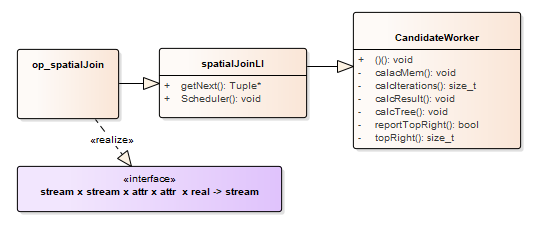
\includegraphics[width=0.75\textwidth]{Bilder/spatialJoin.png}
	\caption{Aufbau des Spatial-Join-Operators (vereinfacht). Gestrichelte Pfeile: Datenfluss; durchgezogene: Instanzen werden erzeugt.}
	\label{img:KlassSJ}
\end{figure}


Wie die anderen Operatoren auch, gliedert sich der Operator in zwei zentrale Bestandteile: ein Scheduling, welches von einer \Fb{LocalInfo}-Klasse ausgeführt wird, und Threads als Worker, in denen der Ergebnisstrom berechnet wird. \autoref{img:KlassSJ} gibt eine Übersicht über das Klassendiagramm des Operators. Anders als bei den bisherigen Operatoren kann eine räumliche Partitionierung nicht sinnvoll ohne Kenntnisse über die R-Relation vorgenommen werden. Die R-Relation wird im Scheduling einmal gescannt und ein zufälliges Sample ihrer \Fb{MBBs} erzeugt, dessen Größe mit der Relationsgröße und der Anzahl genutzter Worker-Threads wächst. Um ein gleich verteiltes Sampling zu erzeugen, werden zunächst die ersten 10 \Fb{MBBs} pro Worker-Thread gespeichert. Anschließend wird eine Zufallszahl erzeugt, die beginnend mit der Anzahl von zuerst gespeicherten \Fb{MBBs} in jedem Durchgang um 1 erhöht wird. Werte zwischen 0 und $10 * Workerthreadzahl - 1$ ersetzen die entsprechende \Fb{MBB}. Um die Größe des Samples an die Größe der Relation anzupassen, wird nach dem Scan von je 1000 Tupeln die Menge der gespeicherten \Fb{MBBs} um 10 erhöht. Nur aus diesen \Fb{MBBs} wird das Gitter für die Partitionierung mittels \Fb{STR} erzeugt. Hierfür wird die Klasse \Fb{IrregularGrid2D} aus der \Fb{SPart}-Algebra verwendet. Ursprünglich hatte diese Klasse nur eine Schnittstelle für Ströme von Rechtecken. Für die Anwendung innerhalb dieses Operators habe ich in der Algebra eine Schnittstelle ergänzt, die einen Vektor von Rechtecken als Parameter erlaubt, um eine direkte Parametrisierung ohne eine Verwendung des Query-Prozessor zu ermöglichen. Da das irreguläre Gitter durch einer Zufallsauswahl erzeugt wurde, kann es sein, dass einige Rechteckrepräsentationen der räumlichen Joinattribute der Relationen außerhalb des Gitters liegen. Deswegen wird das Gitter an seinen Kanten in alle Richtungen bis zu den maximal bzw. minimal möglichen Double-Werten erweitert. Zuerst habe ich für jeden genutzten Kern abzüglich des Kerns für das Scheduling eine Gitterzelle und einen Thread erzeugt. Dementsprechend konnte das Gitter nicht rechteckig sein, sondern bestand nur aus einem Streifen, um unproblematisch auch mit einer Anzahl von Threads umgehen zu können, deren Wurzel keine natürliche Zahl ist. Es hat sich aber gezeigt, dass es wesentlich effizienter ist, deutlich mehr Gitterzellen und Threads als Kerne zur Verfügung stehen zu erzeugen, auch wenn dies das Risiko auf Duplikate erhöht und nicht mehr unbedingt alle Threads durchgehend gleichzeitig arbeiten können. In der abschließend implementierten Version des Operator habe ich ein quadratische Gitter mit der Anzahl genutzter Kerne als Höhe und Breite erzeugt. Dementsprechend werden bei $n$ für die Worker zur Verfügung stehender Kerne $n^2$ Threads erzeugt. Durch die jetzt sehr hohe Anzahl von Gitterzellen ist der von mir implementierte Spatial-Join quasi ein Spatial-Hash-Join, in deren Buckets der Join-Prozess über einen iterativen R-Baum-Algorithmus vorgenommen wird. Für einen eigentlichen  Hash-Algorithmus sind aber die Buckets noch deutlich zu groß.

Die \Fb{MBBs} werden über ein Funktionsobjekt realisiert, um die Fallentscheidung zwischen vergrößerten und nicht vergrößerten \Fb{MBBs} nur einmal implementieren zu müssen. Die R-Relation muss, da sie bereits im Scheduling für die Berechnung des Gitters gescannt wird, temporär gespeichert werden. Hierfür wurde ein Buffer implementiert, der Auslagerungen selbst verwaltet (\autoref{Hilfsstrukturen}. Für die interne Speicherung steht der maximale Speicher des Operators zur Verfügung. Für die Tupelströme steht eine Warteschlangen zur Verfügung. Da eventuell mehr Threads erzeugt werden, als gleichzeitig auf dem System laufen können, wird als Buffer für die Partitionen eine threadsichere Warteschleife verwendet, die in der Lage ist, Daten auszulagern. Da aber mehrere Iterationen über die S-Relation notwendig werden können, wenn die R-Bäume inklusive der Repräsentation der Tupel der R-Relation nicht in den Hauptspeicher passen, kann es sein, dass Ergebnistupel zwischengespeichert werden müssen, bevor sie von der \Fb{GetNext}-Methode der \Fb{LocalInfo}-Klasse abgeholt werden können. Hier hilft es auch nicht, die Workerthreads vom Hauptthread zu entkoppeln, da die \Fb{GetNext}-Methode erst Tupel abholen kann, wenn beide Eingangsrelationen vollständig gelesen worden sind. Eine Möglichkeit, dies zu verhinden, wäre es, jedes mal, wenn der Hauptspeicher vollständig belegt ist, zwischen Scheduling und \Fb{GetNext} zu wechseln. Da dies aber kompliziert umzusetzen ist und sich in anderen Operatoren gezeigt hat, dass die Kommunikation über Bedingungsvariablen sehr teuer ist, wurde ein Ansatz gewählt, der es ermöglicht, den Ergebnisstrom auszulagern.

Für die Datenstrukturen der Worker, vor allem die R-Bäume und Tupelspeicher, wurde in der Implementierung mit wenigen Threads der Speicherplatz global verwaltet. Dies ist aber nicht mehr möglich und sinnvoll, wenn nicht alle Threads von Beginn an arbeiten, da sich dann einige Threads den später startenden den Speicher wegnehmen. Hier einen Ausgleich zu implementieren, lohnt nicht, da durch die Partitionierung über ein irreguläres Gitter eine Gleichverteilung der Speicherbedarfe je Thread angenommen werden kann. Sinnvoll wäre es allerdings als Optimierung des Operators, wenn Threads, die abgeschlossen wurden, ihren Speicher wieder zur Verfügung stellen. Die R-Bäume werden in den Threads angelegt. Ich habe mich gegen einen globalen R-Baum entscheiden, da ich bei einer geringen Anzahl genutzter Kerne von wenigen Duplikaten ausgehe und es deswegen als Vorteil sehe, trotz einer gewissen Redundanz zwischen den R-Bäumen, die Teil-R-Bäume parallel erzeugen zu können. Den Workern stehen insgesamt $\frac{7}{10}$ des Hauptspeichers zur Verfügung, dem globalen Ergebnisbuffer $\frac{1}{10}$ und den Buffern für die R/S-Relation $\frac{2}{16}$ bzw. $\frac{1}{16}$ des Speichers, der einem einzelnen Worker zu Verfügung steht. Sinnvoll wäre es sicher als Verbesserung entweder eine Heuristik zu entwickeln, die die Speicherverteilung aus Threadzahl, Kernzahl und Relationsgröße berechnet oder aber die Speicheraufteilung parametrisierbar macht, um sie dem Nutzer oder dem Optimierer zur Verfügung zu stellen. Die gewählte Speicherverteilung wurden mit Testrelationen optimiert (siehe \autoref{te}). 

Der Join-Prozess selbst ist nicht kompliziert. Aus dem Tupelstrom der R-Relation wird ein interner R-Baum aufgebaut, der so konfiguriert wurde, dass er 4 bis 8 Rechtecke in jedem Knoten aufnehmen kann. Anschließend wird die S-Relation vollständig durchlaufen und Joinkandidaten über eine Suche der \Fb{MBBs} im R-Baum festgestellt. Sofern die R-Relation inklusive des R-Baums nicht mehr in den Hauptspeicher passt, wird der Vorgang wiederholt. Nach einem ersten Durchlauf kann berechnet werden, wie viele Iterationen notwendig sind, wobei immer der maximale Speicherbedarf eines R-Baums vorausgesetzt wird (in der Methode \Fb{calcIterations} wird die Iterationszahl so lange hochgezählt, bis bei der Aufteilung kein Overflow mehr entsteht). Im ersten Durchlauf ist es durchgehend notwendig, den Speicherbedarf zu überwachen, um festzustellen, ab wann die R-Relation nicht mehr in den internen R-Baum geschrieben werden kann, sondern in eine externe Datenstruktur ausgelagert werden muss. Die Berechnung des Speicherbedarfs ist komplizierter als bei den anderen Operatoren, da der Speicherverbrauch des R-Baums nicht linear wächst. Allerdings stellt die genutzte Implementierung eines internen R-Baums von \Fb{Secondo} für diese Berechnung eine Methode zur Verfügung.

Duplikate machen auf zwei Ebenen Probleme. Einerseits soll das Ergebnis frei von Duplikaten sein. In \autoref{entw:spatial} habe ich bereits erläutert, dass diese in der Entstehung über ihre Position innerhalb des Gitters erkannt werden können, also erst gar nicht als Joinkandidaten an den Ergebnisstrom weitergegeben werden. Für diesen Zweck habe ich die Methoden \Fb{topright} und \Fb{reportTopright} implementiert. Andererseits bereiten Duplikate Probleme bei der Löschung von Tupeln, die keine Joinkandidaten sind. Anders als bei den beiden anderen Operatoren dürfen Tupel erst gelöscht werden, wenn sie in allen Gitterzellen, in denen sie vorkommen, getestet wurden. Für diesen Zweck muss hier der Referenzzähler der Tupel-Klasse genutzt werden, um sicherzustellen, dass ein Tupel erst gelöscht wird, wenn keine Referenz in anderen Threads mehr vorhanden ist.

\subsubsection{Spatial-Join Refinement Step}
\label{impl:refinement}

Der \Fb{MThreadFilter}-Operator ist analog zu dem nicht parallelen Filter-Operators angelegt und ist damit vielseitiger als ausschließlich für den Refinement Step eines Spatial-Joins zu verwenden. Übergeben wird eine beliebige Funktion als Prädikat. Die Signatur des Operators ist: \newline
$stream~x~fun \longrightarrow stream$

Auch wenn die Architektur des Operators simpel ist, hat die Implementierung große Schwierigkeiten bereitet und konnte nicht zufriedenstellend gelöst werden. Vor allem liegt das an Problemen mit der Threadsicherheit von Zugriffen auf \Fb{FLOBs}.

Bereits das Type-Mapping ist kompliziert, da anders als in der Singlethread-Version die übergebende Funktion nicht direkt im Queryprozessor genutzt werden kann, sondern für jeden Thread ein eigener Operatorenbaum für einen eigenen Query-Prozessor konstruiert werden muss. Für diesen Zweck ist es notwendig, dass die Argumente, das heißt in diesem Fall die Funktion, an das Type-Mapping übergeben wird. Also wird für den Operator das Parameter \Fb{SetUsesArgsInTypeMapping} gesetzt. Die Attribute der Funktion werden darauf getestet, ob sie im Eingangsstrom vorkommen und das Ergebnis des Prädikats muss für einen Filter vom Typ Boolean sein. Die Funktion wird als Textobjekt (\Fb{FText}) mithilfe des Append-Mechanismus an das Value-Mapping übergeben. Im Scheduling kann die Funktion dann von einem Textobjekt in eine \Fb{ListExpr} umgewandelt werden, um die jeweiligen Operatorenbäume für die Queryprozessoren der Threads zu erzeugen.

Die Implementierung hat mehrere Ziele: Die möglichst vollständige Berechnung, ob Joinkandidaten auch bei einer genauen Auswertung der Prädikate mit den räumlichen Attributen weiterhin verschmolzen werden müssen oder allgemein, ob die Filter-Prädikate als wahr ausgewertet werden, soll in den Threads vorgenommen werden, da dieser Schritt sehr hohe Kosten verursacht. Eine Synchronisierung und damit Serialisierung gerade der teuren Berechnung soll vermieden werden. Der Operator soll nicht blockierend sein, das heißt es sollen direkt von Filter durchgelassene Tupel an den Ergebnisstrom ohne eine temporäre Speicherung übergeben werden. Darüber hinaus sollen die Threads möglichst nicht pausieren, dass heißt Ein- und Ausgabestrom sollen parallel zur Berechnung der Filterprädikate in den Threads verarbeitet werden.

Durch diese Ziele wird die konkrete Implementierung des Operators deutlich komplexer als die Singlethread-Version, da mehrere Threads durchgehend über einen Eingabestrom verfügen müssen und gleichzeitig der Ergebnisstrom weitergeleitet werden muss. Probleme liegen vor allem in der Partitionierung und im Scheduling im Master-Thread, nicht so sehr im Filteralgorithmus in den Worker-Threads. Mein erster Ansatz versuchte, die Verteilung nach Round Robin in einen eigenen Thread auszulagern, damit die Verteilung und Ergebnisweitergabe über die \Fb{\Fb{GetNext}}-Methode parallel und damit beide Ströme kontinuierlich fließen können. Dieser Ansatz, der voraussetzt, dass die Threads vom Hauptthread entkoppelt werden, ist allerdings schwierig in der Synchronisation vor allem bei der Destruktion von Objekten und führte zu undefiniertem Verhalten vor Allem bezüglich des Schließen des Eingangsstroms und der Zerstörung der Queryprozessoren. Auch trat bereits ein Problem auf, welches ich leider nicht vollständig lösen konnte: Vermutlich durch eine fehlende Synchronisation von nicht zulässigen gleichzeitigen Zugriffen auf die Berkelely-DB wurde ein Commit verhindert, da entweder offene Zeiger auf Objekten der Queryprozessoren vorhanden waren oder im Commit noch Sperren bestanden, die teils zu einer Ausnahme führen, teils zu einem Deadlock während des Commits.

Eine erste Vereinfachung versuchte noch die Parallelität von Strömen und Prädikats"-berechnungen aufrechtzuerhalten, aber die Probleme zu reduzieren, die dadurch entstanden, wenn der Eingangsstrom in einem eigenen Thread behandelt wird und der Aufruf der Destruktoren der Threads schwer zu koordinieren ist. Jetzt alternierte der Master-Thread zwischen einer Partitionierungs- und der \Fb{GetNext}-Methode. Da nicht vorauszusehen ist, wie groß die Selektivität des Filters ist, musste die \Fb{GetNext}-Methode so implementiert werden, dass sie nur so lange auf Ergebnisse wartet, bis die Buffer, die als threadsichere Warteschlange implementiert sind, fast leer sind. Eine weitere Synchronisation wurde notwendig, um einen Deadlock zu verhindern, wenn der Eingangsstrom erschöpft ist. Zuerst wurden die Queryprozessoren, die die Filterprädikate in den Threads auswerten, auch in diesen erzeugt, was zu Nebeneffekten führte, wenn diese zerstört wurden. Deswegen wurden die Queryprozessoren direkt in der \Fb{LocalInfo}-Klasse erzeugt und in deren Destruktor zerstört. Mit diesem Ansatz gelang es, Probleme auf den Commit zu reduzieren, auch wenn eine große Relation mit \Fb{FLOBs} verarbeitet wurde. Abschließend implementiert wurde eine einfache Lösung, die gleichzeitig am stabilsten lief. Eine Round-Robin-Partitionierung wurde dadurch vorgenommen, dass die Partitionierung nicht im Master-Thread vorgenommen wurde, sondern die Worker sich synchronisiert Tupel direkt aus dem Eingangsstrom entnehmen. Dieser Ansatz teilt die Vorteile des aufwändig zu synchronisierenden Threads für die Partitionierung, aber bedeutet wenig Aufwand für die Synchronisierung und ermöglicht auch einen Lastenausgleich, da Tupel aus dem Strom immer nach Bedarf entnommen werden.

Eine genaue Lokalisierung der auftretenden Fehler war schwierig, da sie sich erst im Commit, also nach Abschluss der Filteroperators, aber auch des vollständigen Querybaums manifestierten. Der implementierte Operator selbst lief unter Erzeugung des richtigen Ergebnis vollständig durch. Der Fehler trat auch bei Verwendung nur eines Thread auf, also ist die Ursache wahrscheinlich kein Synchronisationsproblem zwischen den Prädikatsauswertungen. Eine Vermutung ist es, dass neben den Queryprozessoren der Threads teils Prozesse außerhalb der Threads auch auf \Fb{FLOBs} der Tupelattribute, die in das Prädikat eingehen, zugreifen oder aber eine fehlende Synchronisierung zwischen unterschiedlichen Zugriffen auf die Speicherschicht über den Storage-Manager. Um die Möglichkeit gleichzeitiger Zugriffe einzuschränken, habe ich einen Performanceverlust in Kauf genommen, indem so synchronisiert wurde, dass entweder nur die Prädikatauswertung oder nur die Verarbeitung des Tupelstroms ablaufen darf. Eine Synchronisation wurde mithilfe einer Bedingungsvariable und Mutexen vorgenommen, führte aber auch nicht zu einer fehlerfreien Funktion des Operators. Auch ein letzter Versuch, \Fb{Secondo} ohne Commit zu verwenden, führte zwar dazu, dass deutlich seltener und erst bei größeren Relationen Fehler auftraten, aber immer noch kam es im Abschluss der Abfrage, die den Filter beinhaltete, gelegentlich zu Abstürzen. Darüber hinaus traten ohne Commit auch Abstürze durch fehlerhaft konfigurierte Zugriffe des Flob-Managers auf, wahrscheinlich, da dort Zeiger durch konkurrierende Zugriffe ungültig geworden sind.

Ein letzter Versuch der Fehlerbehebung war es, den Queryprozessor im Worker-Threads mehrmals zu erzeugen und wieder zu zerstören. Dieser Ansatz hätte, wenn dies nicht allzu häufig vorgenommen werden muss, zu einem Operator führen können, der zwar nicht optimal Parallelität ausnutzt, aber trotzdem schneller als die Singlethread-Version ist, sofern die Auswertung der Prädikate entsprechend teuer ist. Die Idee begründet sich darin, dass es erst bei relativ großen Relationen zu dem Commit-Fehler kommt. Allerdings funktionierte dieser Ansatz nur, wenn maximal 20 Tupel ausgewertet wurden, bevor der Queryprozessor zerstört und wieder neu aufgebaut wird. Damit war auch dieser Ansatz keine Alternative.

\section{Test und Experimente} 
\label{te}

Im folgenden Abschnitt werden umfangreiche Tests der Operatoren diskutiert und ihr Verhalten unter unterschiedlichen Bedingungen untersucht. Da hier nicht ein abstraktes Laufzeitverhalten betrachtet wird, sondern die konkrete Laufzeit der Implementierung auf einem spezifischen System, beschreibe ich dieses kurz, um die Messergebnisse kontextualisieren zu können. Da die Effizienz vor allem durch einen Vergleich mit Singlethread-Operatoren bewertet wird, geht es nicht vor allem um die einzelnen Messergebnisse, sondern um eine Beschleunigung durch Parallelisierung gleicher Anfragen. 

Entwickelt wurde auf einem \Fb{openSuse Leap}~15.0 System mit einem \Fb{AMD~6300~FX} Prozessor (L1-Cache: je Kern 16 KB Daten \& je Modul 64 KB Instruktionen, L2-Cache je Modul 2048 KB mit Prozessortakt, L3-Cache 8 MB mit Northbridge-Takt, 3,5/3,8/4,1 GHz), 16 GB Arbeitsspeicher und einer SSD. Anzumerken ist, dass der Prozessor zwar über
sechs Integer-Cluster, aber nur über drei Gleitkomma-Einheiten verfügt. Zwei Kerne sind je zu einem Modul zusammengefasst.

Die Laufzeitmessung  habe ich ausschließlich auf einem Windows 2016 Server mit deutlich besserer und aktuellerer Hardware vorgenommen, auf dem Ubuntu 20.04~LS als Gast-Betriebssystem unter VMWare~Workstation~Pro~16 läuft. Der Server verfügt über zwei \Fb{Xeon Gold 6128} Prozessoren mit je sechs Kernen (L1: 384 KB, L2 6 MB, L3 19,25 MB, 3,7/3,54 GHz) sowie Hyperthreading, 396 GB Arbeitsspeicher und zwei SSDs. Dem Gast-Betriebssystem stehen insgesamt 2~x~6 Kerne und 64 GB Arbeitsspeicher zur Verfügung.

Gegliedert ist dieses Kapitel in zwei Teilabschnitte: Zuerst wird es darum gehen zu ermitteln, ob meine Operatoren den gestellten Zielen entsprechen und gut funktionieren. Im Konkreten bedeutet dies die Korrektheit des Operators, dessen Robustheit und Effizienz. Dem folgen Experimente, in denen ich das Verhalten der Operatoren unter unterschiedlichen Bedingungen beobachte, vergleiche und diskutiere. Die Experimente dienen darüber hinaus, mögliche Verbesserungspotentiale und Probleme meiner Implementierung zu identifizieren. Alle Tests und Experimente wurden mit \Fb{Secondo} ohne Commit (\Fb{SecondoTTYNT} ausgeführt, da die Operatoren dann bei \Fb{Flobs} etwas stabiler arbeiten. 

\begin{itemize}
	\item Korrektheit: keine Speicherlecks (Test mit \Fb{-{}-valgrindlc}); richtiges Ergebnis bei unterschiedlichen Anfragen, bei denen sichergestellt ist, dass alle Programmbereiche durchlaufen worden sind; Verhalten bei \Fb{FLOBs}.
	\item Robustheit meint das Funktionieren mit unkorrekten bzw. nicht sinnvollen Parametern: Werden nur Parameter zugelassen, mit denen der Operator funktioniert? Verhalten bei leeren Relationen oder wenn die Ergebnisrelation leer ist. Verhalten bei extremen Verteilungen.
	\item Effizienz: Vergleich mit der Singlethread-Version bei Nutzung verschiedener Anzahl von Kernen. 
\end{itemize}

Die Experimente haben verschiedene Aufgaben: Es soll das genaue Verhalten der Operatoren bei unterschiedlichen Parametern, vor allem bezüglich Relationsgröße, Verteilungen und Threadzahl, untersucht werden. Es wird versucht, optimale Einstellungen interner Parameter zu ermitteln -- beispielsweise Speicherverteilung zwischen unterschiedlichen Datenstrukturen, Konfiguration des R-Baums und die Anzahl von Buckets in den Hashtabellen. Ziel ist es, die Operatoren zu optimieren und ungünstige Entscheidungen in der Implementierung sowie grundsätzliche Probleme bei der Parallelisierung in \Fb{Secondo} zu identifizieren.

\begin{figure}
	\centering
	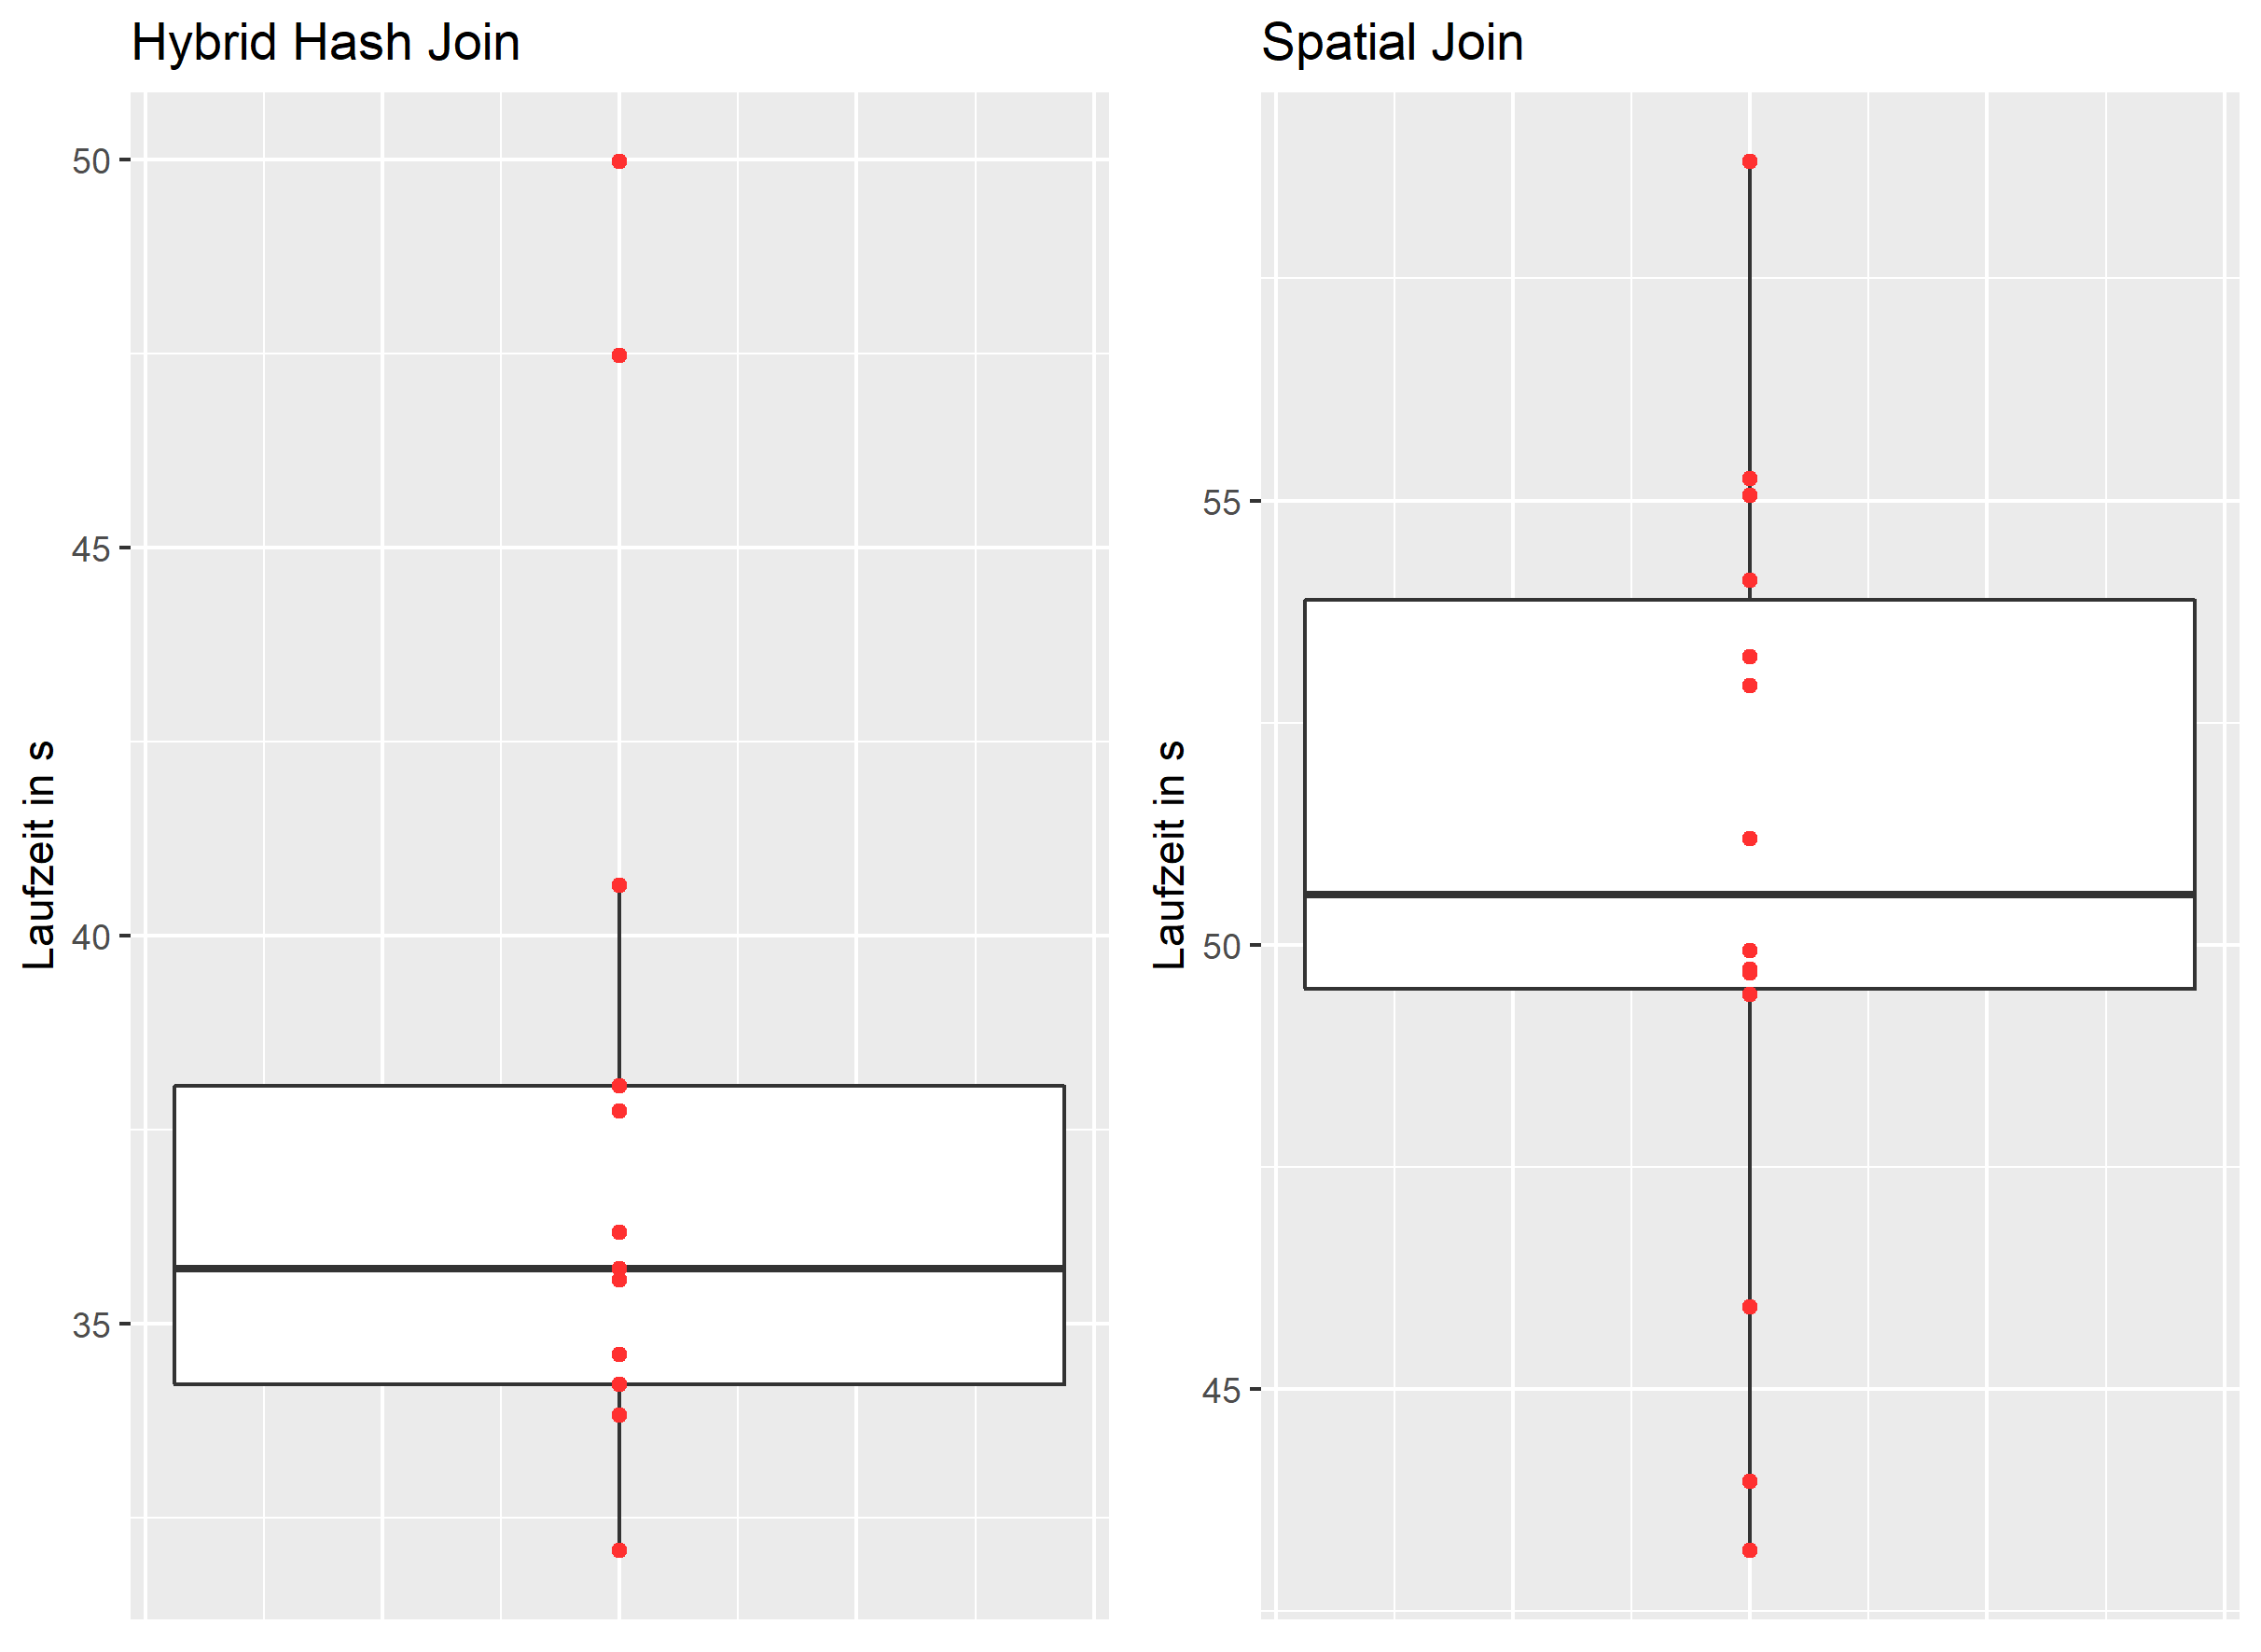
\includegraphics[width=0.70\textwidth]{Bilder/streuung.png}
	\caption{Mehrfache Ausführung der gleichen Hash-Joins $roads \bowtie roads$ und Spatial-Joins $roads \bowtie waterways$.}
	\label{img:streuung}
\end{figure}

Sofern Laufzeiten für die Effizienztests und Experimente gemessen werden, wird die Ausgabe der vergangenen Zeitdauer (\Fb{elapsed time}) und die CPU-Zeit nach Ausführung einer Anfrage in \Fb{SecondoTTYBDB} ausgewertet. Die vergangene Zeitdauer ist die Differenz der Zeitstempel beim Start der Anfrage und bei Abschluss. Die CPU-Zeit ist die Zeit, die vom Prozessor verbraucht wird, also die reine Berechnungszeit ohne die Zeit, die der Prozessor beispielsweise auf I/O-Operationen oder andere Prozesse wartet. Da jeder Thread CPU-Zeit verbraucht, ist diese für einen Vergleich mit Singlethread-Operatoren nicht geeignet. Der Koeffizient aus vergangener Zeit und CPU-Zeit gibt aber Hinweise darauf, wie gut eine Parallelisierung gelungen ist. Ein optimaler Koeffizient wäre $1 / n$ bei $n$ verwendeten Kernen, was aber wegen des Schedulings bzw. allgemein des Overheads und der Verwendung weiterer Operatoren in der Anfrage nie erreicht wird. Wenn der Koeffizient sich diesem Wert nähert, würden während der gesamten Anfragebearbeitung alle Kerne dauerhaft genutzt werden.

Im Gegensatz zu vielen Singlethread-Operatoren ist die Laufzeit bei Verwendung von Multithreading nicht stabil, da die Partitionierung nicht immer identisch vorgenommen wird und die Synchronisation nicht vorhersagbar ist. \autoref{img:streuung} zeigt die Verteilung von Laufzeiten bei mehrmaliger Ausführung eines Spatial-Joins und eines Hash-Joins. Dieses Verhalten der Operatoren macht die Interpretation der Messergebnisse schwierig, insbesondere wenn keine eindeutige Tendenz zu erkennen ist. Allerdings wurden alle Tests mehrfach ausgeführt und per Augenschein überprüft, ob Ergebnisse stark variieren. Zumindest Extremwerte wurden so versucht auszuschließen.  

Für die Testes der Operatoren verwende ich den Berlin-Datensatz von Open Streetmap, der mit dem Stand 7.1.2020 heruntergeladen worden ist (siehe \autoref{tab:testRel})\footnote{\url{http://download.geofabrik.de/europe/germany/berlin.html}} sowie die \Fb{berlintest}-Datenbank, die \Fb{Secondo} beiliegt.

\begin{table}
	\centering
\begin{tabular}{|c|c|c|c|}
	\hline
	\rowcolor{gray!30}
	Tabelle & Anzahl Tupel & Quelle & räumlicher Datentyp  \\ 
	\hline 
	buildings & 502.309 & gis\_osm\_buildings\_a\_free\_1 & region \\ 
	\hline 
	landuse & 29.341 & gis\_osm\_landuse\_a\_free\_1 & region \\ 
	\hline 
	natural & 116 & gis\_osm\_natural\_a\_free\_1 & region \\ 
	\hline 
	natural2 & 162.112 & gis\_osm\_natural\_free\_1 & point \\ 
	\hline
	places & 108 & gis\_osm\_places\_free\_1 & region \\ 
	\hline 
	pois & 66.123 & gis\_osm\_pois\_free\_1  & point \\ 
	\hline 
	roads & 181.685 & gis\_osm\_roads\_free\_1 & line \\ 
	\hline
	traf & 40.650 & gis\_osm\_traffic\_free\_1  & point \\ 
	\hline 
	waterways & 2104 & gis\_osm\_waterways\_free\_1 & line \\ 
	\hline
	strassen & 3212 &  berlintest & line \\ 
	\hline
	WFlaechen & 85 &  berlintest & region \\ 
	\hline 
	WStrassen & 21 &  berlintest & line \\ 
	\hline 
	Plaetze & 201 &  berlintest & point \\ 
	\hline 
	Orte & 506 & berlintest & keine \\ 
	\hline
	plz & 41267 & berlintest & keine \\ 
	\hline 
\end{tabular}
\caption{\label{tab:testRel} Übersicht über in Tests und Experimenten verwendeten Relationen.}
\end{table}

Da es mehrfach Probleme mit \Fb{FLOBs} gab, nutze ich auch Versionen der Relationen, in denen Attribute des Typs \Fb{FText} in \Fb{string} umgewandelt worden sind. Kennzeichen für diese Relationen ist das Postfix \Fb{\_str}.

\subsection{Funktionstests}

\subsubsection{mThreadedSort}

Auf Korrektheit wird auf zweierlei Art und Weise getestet: Es ist notwendig, dass ein Test mit \Fb{--valgrindlc} ohne Fehler abläuft und das Ergebnis muss den Erwartungen entsprechen. Das heißt, eine Relation muss entsprechend der Sortierattribute und Reihenfolge korrekt sortiert werden. Eine Korrektheit kann nur abschließend festgestellt werden, wenn garantiert ist, dass der Programmcode des Operators in der Summe der Tests vollständig durchlaufen worden ist. Kontrolliert habe ich dies mit Ausgaben an die Konsole, die in der endgültigen Version des Operators entfernt worden sind. Vollständig durchlaufen wird der Programmcode, wenn die Relationen ausreichend groß sind, sodass Läufe ausgelagert werden müssen (bzw. wenig Hauptspeicher zur Verfügung gestellt werden muss) und wenn mehr als zwei Läufe in der suboptimalen Phase verschnitten werden müssen. In der postoptimalen Phase sollen die Feeder mit ein und zwei Eingängen getestet und ein Mergepipeline-Baum konstruiert werden, der nicht lediglich Blätter und eine Wurzel enthält. Dementsprechend wird mit 3, 4 und 6 Threads getestet \footnote{Der Hauptthread, in dem der \Fb{Secondo}-Kern und damit auch das Scheduling läuft, zählt immer mit.}. Darüber hinaus wird mit einer Threadanzahl getestet, die deutlich über der Kernzahl des System liegt. In diesem Fall Threads zwischenzeitlich pausieren müssen. Für die Performance ist dies allerdings nicht sinnvoll, aber auch in diesem Fall muss der Operator korrekt funktionieren, da unter Anwendungsbedingungen nicht unbedingt bekannt ist, wie viele Kerne genutzt werden können oder eventuell durch andere Programme verwendet werden.

Mit \Fb{-{}-valgrindlc} terminiert der Operator nur in einem Fall mit einem Speicherloch, nämlich sofern der Operator nicht vollständig speicherintern abläuft. Ein Zeiger auf eine \Fb{CcInt} wird nicht gelöscht. Dies ist allerdings kein Fehler meines Operators, sondern ein bekannter Fehler des Queryprozessors, der auftritt, wenn der Queryprozessor Konstanten verwendet. Sofern mehr Threads verwendet werden als Kerne zur Verfügung stehen, kann es zu einem Deadlock kommen. Deswegen wird die verwendete Threadzahl auf die maximale Anzahl von Kernen des Systems reduziert, sofern sie höher eingestellt worden ist. 

\begin{minipage}{0.95\textwidth}
	\begin{lstlisting}[caption={Beispiel Testqueries für den Sort-Operator.}, label=list:testsort]
	query (roads_str feed mThreadedMergeSort[NameStr] {memory 12} project[NameStr]) = (roads_str feed sortby[NameStr] project[NameStr]) 
	\end{lstlisting}
\end{minipage}

Korrektheit wird mit unterschiedlich großen Relationen, der Memory-Option, um sicherzustellen, dass alle Persistierungsstrukturen durchlaufen werden und mit unterschiedlichen vielen Threads getestet (siehe \autoref{tab:testSort}). Im Unterschied zu den anderen implementierten Operatoren dieser Algebra läuft nicht in jedem Thread der gleiche Algorithmus ab. Der Aufbau der Mergepipeline in der postoptimalen Phase unterscheidet sich bezüglich der Anzahl genutzter Threads. Unterschiede bestehen zwischen einer geraden und ungeraden Threadzahl und der Notwendigkeit von Zwischenschritten, die erst ab 5 Threads (plus einen Hauptthread) verwendet werden müssen. Wichtig ist es hier, die Ergebnisrelation auf die Sortierattribute zu projizieren (siehe Beispielanfrage \autoref{list:testsort}), da meine Implementierung eines Multithread-Sort nicht die Reihenfolge der Relation aufrecht erhält, das heißt, die Ergebnisrelation kann sich bei Duplikaten in den Sortierattributen in der Reihenfolge nicht für die Sortierung genutzter Attribute unterscheiden. Es wird lediglich garantiert, dass richtig sortiert wird, aber die Reihenfolge in den Nicht-Sortierattributen kann bei jeder Abfrage auch bei genau identischen Parametern unterschiedlich sein. Zusätzlich werden die Ergebnisse überprüft, wenn mehr als ein Sortierattribut verwendet wird und für eine invertierte Sortierreihenfolge.

\begin{table}
	\centering
\begin{tabular}{|c|c|c|c|}
	\hline
	\rowcolor{gray!30} 
	Threads\footnotemark & speicherintern & project & Ergebnis \\ 
	\hline 
	3 & ja & ja & true \\ 
	\hline 
	3 & nein & ja & true \\ 
	\hline 
	4 & ja & ja & true \\ 
	\hline 
	4 & nein & ja  & true \\ 
	\hline 
	6 & ja & ja & true \\ 
	\hline
	6 & nein & ja & true \\ 
	\hline
	6 & ja & nein & false \\ 
	\hline
	\rowcolor{gray!30}
	\multicolumn{3}{|c|} {Sortierattribute} & \\ 
	\hline 
	\multicolumn{3}{|c|} {Oneway, Maxspeed, Fclass, NameStr} &  true \\ 
	\hline 
	\multicolumn{3}{|c|} {NameStr, FALSE} &  true\\ 
	\hline 
\end{tabular}
\caption{\label{tab:testSort} Threadzahl und zur Verfügung stehender Hauptspeicher sowie  Sortierattribute und Reihenfolge beim Merge-Sort.}
\end{table}

\footnotetext{inkl. Hauptthread und Scheduling. Für das Sortieren und die Merge-Pipeline steht also ein Thread weniger zur Verfügung.}

Der Operator gibt keine korrekten Ergebnisse aus, sofern \Fb{FLOBs} Sortierattribute sind -- im konkurrierenden Zugriff werden die Objekte fehlerhaft in den Speicher eingelesen und dementprechend nicht korrekt verglichen. Wenn aber eine Relation lediglich \Fb{FLOBs} als Attribute hat, diese aber keine Sortierkriterien sind, ist die Ausgabe richtig.

Im folgenden werde ich den Operator auf Robustheit testen. Die Ergebnisse sind in \autoref{tab:testSortRobust} zusammengestellt. Als Beispiel für eine spezielle Verteilung der Eingangsrelation wird mit einer vollständig sortierten Eingangsrelation getestet. In diesem Fall müssen auch bei sehr großen Relationen keine Daten temporär gespeichert werden. Vergleichbares gilt, wenn nach Attributen sortiert wird, die nur sehr wenige Ausprägungen haben, wobei hier nicht garantiert ist, dass keine Daten zwischengespeichert werden müssen. Leere Eingangsströme bzw. Relationen als Eingang, die nur sehr wenige Tupel beinhalten, können dazu führen, dass alle oder einzelne Sortierthreads keine Daten zugewiesen bekommen. Die weiteren Tests betreffen eine Parametrisierung, die nicht sinnvoll oder fehlerhaft ist und vom Type-Mapping abgefangen bzw. behandelt wird. Für alle Operatoren wird erst ab mindestens drei Kernen garantiert, dass sie funktionieren --  zwei Worker-Thread oder mehr und ein Hauptthread inklusive Scheduling. Der Sort-Operator funktioniert nicht richtig, wenn wesentlich mehr Threads verwendet werden, als das System Kerne zur Verfügung hat. Dann kann es zu Deadlocks in der Mergepipeline kommen. Da in diesem Fall kein Performancevorteil zu erwarten ist, wird die Threadzahl dann auf die maximale Kernzahl des Systems gesetzt. Sofern keine Sortierreihenfolge angegeben ist, wird automatisch aufwärts sortiert (\Fb{TRUE}). Eine Besonderheit in dem Type-Mapping dieses Operators ist es, dass Sortierattribute, die nicht Teil der Relation sind, lediglich ignoriert werden. Das Type-Mapping gibt allerdings einen Fehler aus, wenn gar kein gültiges Sortierattribut angegeben wird. Das letzte Testbeispiel zeigt, wie eine Attributliste mit Fehlern umgewandelt wird.

\begin{table}
	\centering
	\begin{tabular}{|p{7.5cm}|p{7.5cm}|}
		\hline
		\rowcolor{gray!30}
		Test & Ergebnis \\
		\hline
		Eingang vollständig vorsortiert & TRUE, keine Anlage temporärer Dateien \\
		\hline
		Sortierattribut Maxspeed,\newline wenig Ausprägungen & TRUE  \\
		\hline
		mit 2 Kernen & only works with $\geq$ 3 threads  \\ 
		\hline
		mit 20 Kernen & uses max system cores only: 6 \\ 
		\hline
		Eingangsstrom leer & leere Ergebnisrelation \\ 
		\hline
		Eingangsstrom 2 Tupel & Ergebnisstrom 2 Tupel \\ 
		\hline
		Eingang kein Strom & first arg is not a tuple stream \\ 
		\hline
		automatische Setzung Sortierreihenfolge & nicht angegebenes TRUE wird ergänzt \\ 
		\hline
		Sortierattribut nicht Teil der Relation & did not find any attribute \\ 
		\hline
		Sortierreihenfolge nicht boolean & automatische Setzung TRUE \\ 
		\hline
		kein Sortierattribut & list corrupt \\
		\hline
		Oneway, NoAttr, FALSE, Maxspeed,\newline Fclass, FALSE, NameStr &  Oneway TRUE Maxspeed TRUE\newline Fclass FALSE NameStr TRUE \\
		\hline
\end{tabular}
	\caption{\label{tab:testSortRobust}Robustheit Merge-Sort.}
\end{table}

Die Effizienz wird durch den Vergleich mit dem Operator Fb{sortby} überprüft. Die Beispielrelation \Fb{roads\_str} wird nach dem Straßennamen sortiert (siehe \autoref{img:sortKern}) und darüber hinaus nach mehreren Sortierattributen (\Fb{Fclass, Oneway, Bridge, Tunnel, Code, NameStr}) (siehe \autoref{img:sortKernMf}). Bei der Nutzung von drei Kernen ist die von mir implementierte Variante schneller als die Single-Thread-Version, sofern nach mehreren Attributen sortiert wurde, und ungefähr gleich schnell, wenn nur nach einem Attribut sortiert wurde. Damit bei einer Sortierung nach mehreren Attributen wirklich viele Vergleiche notwendig sind, muss die Reihenfolge der Sortierattribute so gewählt werden, dass die zuerst zu berücksichtigen Attribute sehr wenige Ausprägungen haben, da der Operator nur weitere Vergleiche vornimmt, wenn die bisherigen in den zu vergleichenden Tupeln identisch waren. Auch wenn dieses Vorgehen für eine gute Performance einer Abfrage nicht sinnvoll ist, geht es mir hier darum zu vergleichen, wie sich der Operator verhält, wenn die Sortierkosten pro Tupel höher sind und damit mehr Kosten im Thread bei gleichen Kosten für das Scheduling entstehen.  

Bemerkenswert ist es, dass sich das Laufzeitverhalten mit der Anzahl genutzter Kerne verschlechtert und zwar sprunghaft ab drei bzw. vier Kernen, wobei anschließend wieder eine leichte Verbesserung eintritt. Einige Faktoren tragen zu diesem Verhalten bei: Nur bei $4, 8, 16, \ldots$ Worker-Threads \footnote{Ein Kern wird bei allen Operatoren für das Scheduling verwendet} entspricht die Merge-Pipeline einem ausgeglichenen Baum -- in den anderen Fällen kann es dementsprechend zu Wartezeiten in den entsprechenden Knoten der Pipeline kommen. Eine Vorsortierung wird bei der Nutzung von vielen Threads nicht gut genutzt, da vorsortierte Folgen auf unterschiedliche Worker verteilt werden. Abschließend vermute ich, dass der Flaschenhals vor allem in der Synchronisation der Warteschlangen liegt, die als Datenaustauschstruktur zwischen den einzelnen Elementen der Merge-Pipeline dient, da das Laufzeitverhalten vor allem an den Punkten schlechter wird, an denen eine Ebene in der Merge-Struktur hinzugefügt wird. 

Eine weitere Kennzahl unterstützt diese Interpretation: Der Koeffizient aus vergangener Zeit und CPU-Zeit, der als Maß für die Parallelisierung genommen werden kann (sofern andere Einflüsse wie I/O-Operationen gleich bleiben) sinkt von drei (0,69) zu zehn Kernen (0,40) deutlich, aber nicht linear, sondern mit der Anzahl genutzter Kerne langsamer. Da auch die genutzte CPU-Zeit steigt, ist davon auszugehen, dass bei der Nutzung von mehr Kernen deutlich größere Verluste durch das Overhead für die Parallelisierung eintreten. 

\begin{figure}
	\centering
	\subfloat[\Fb{roads\_str} nach dem Straßennamen\label{img:sortKern}]{{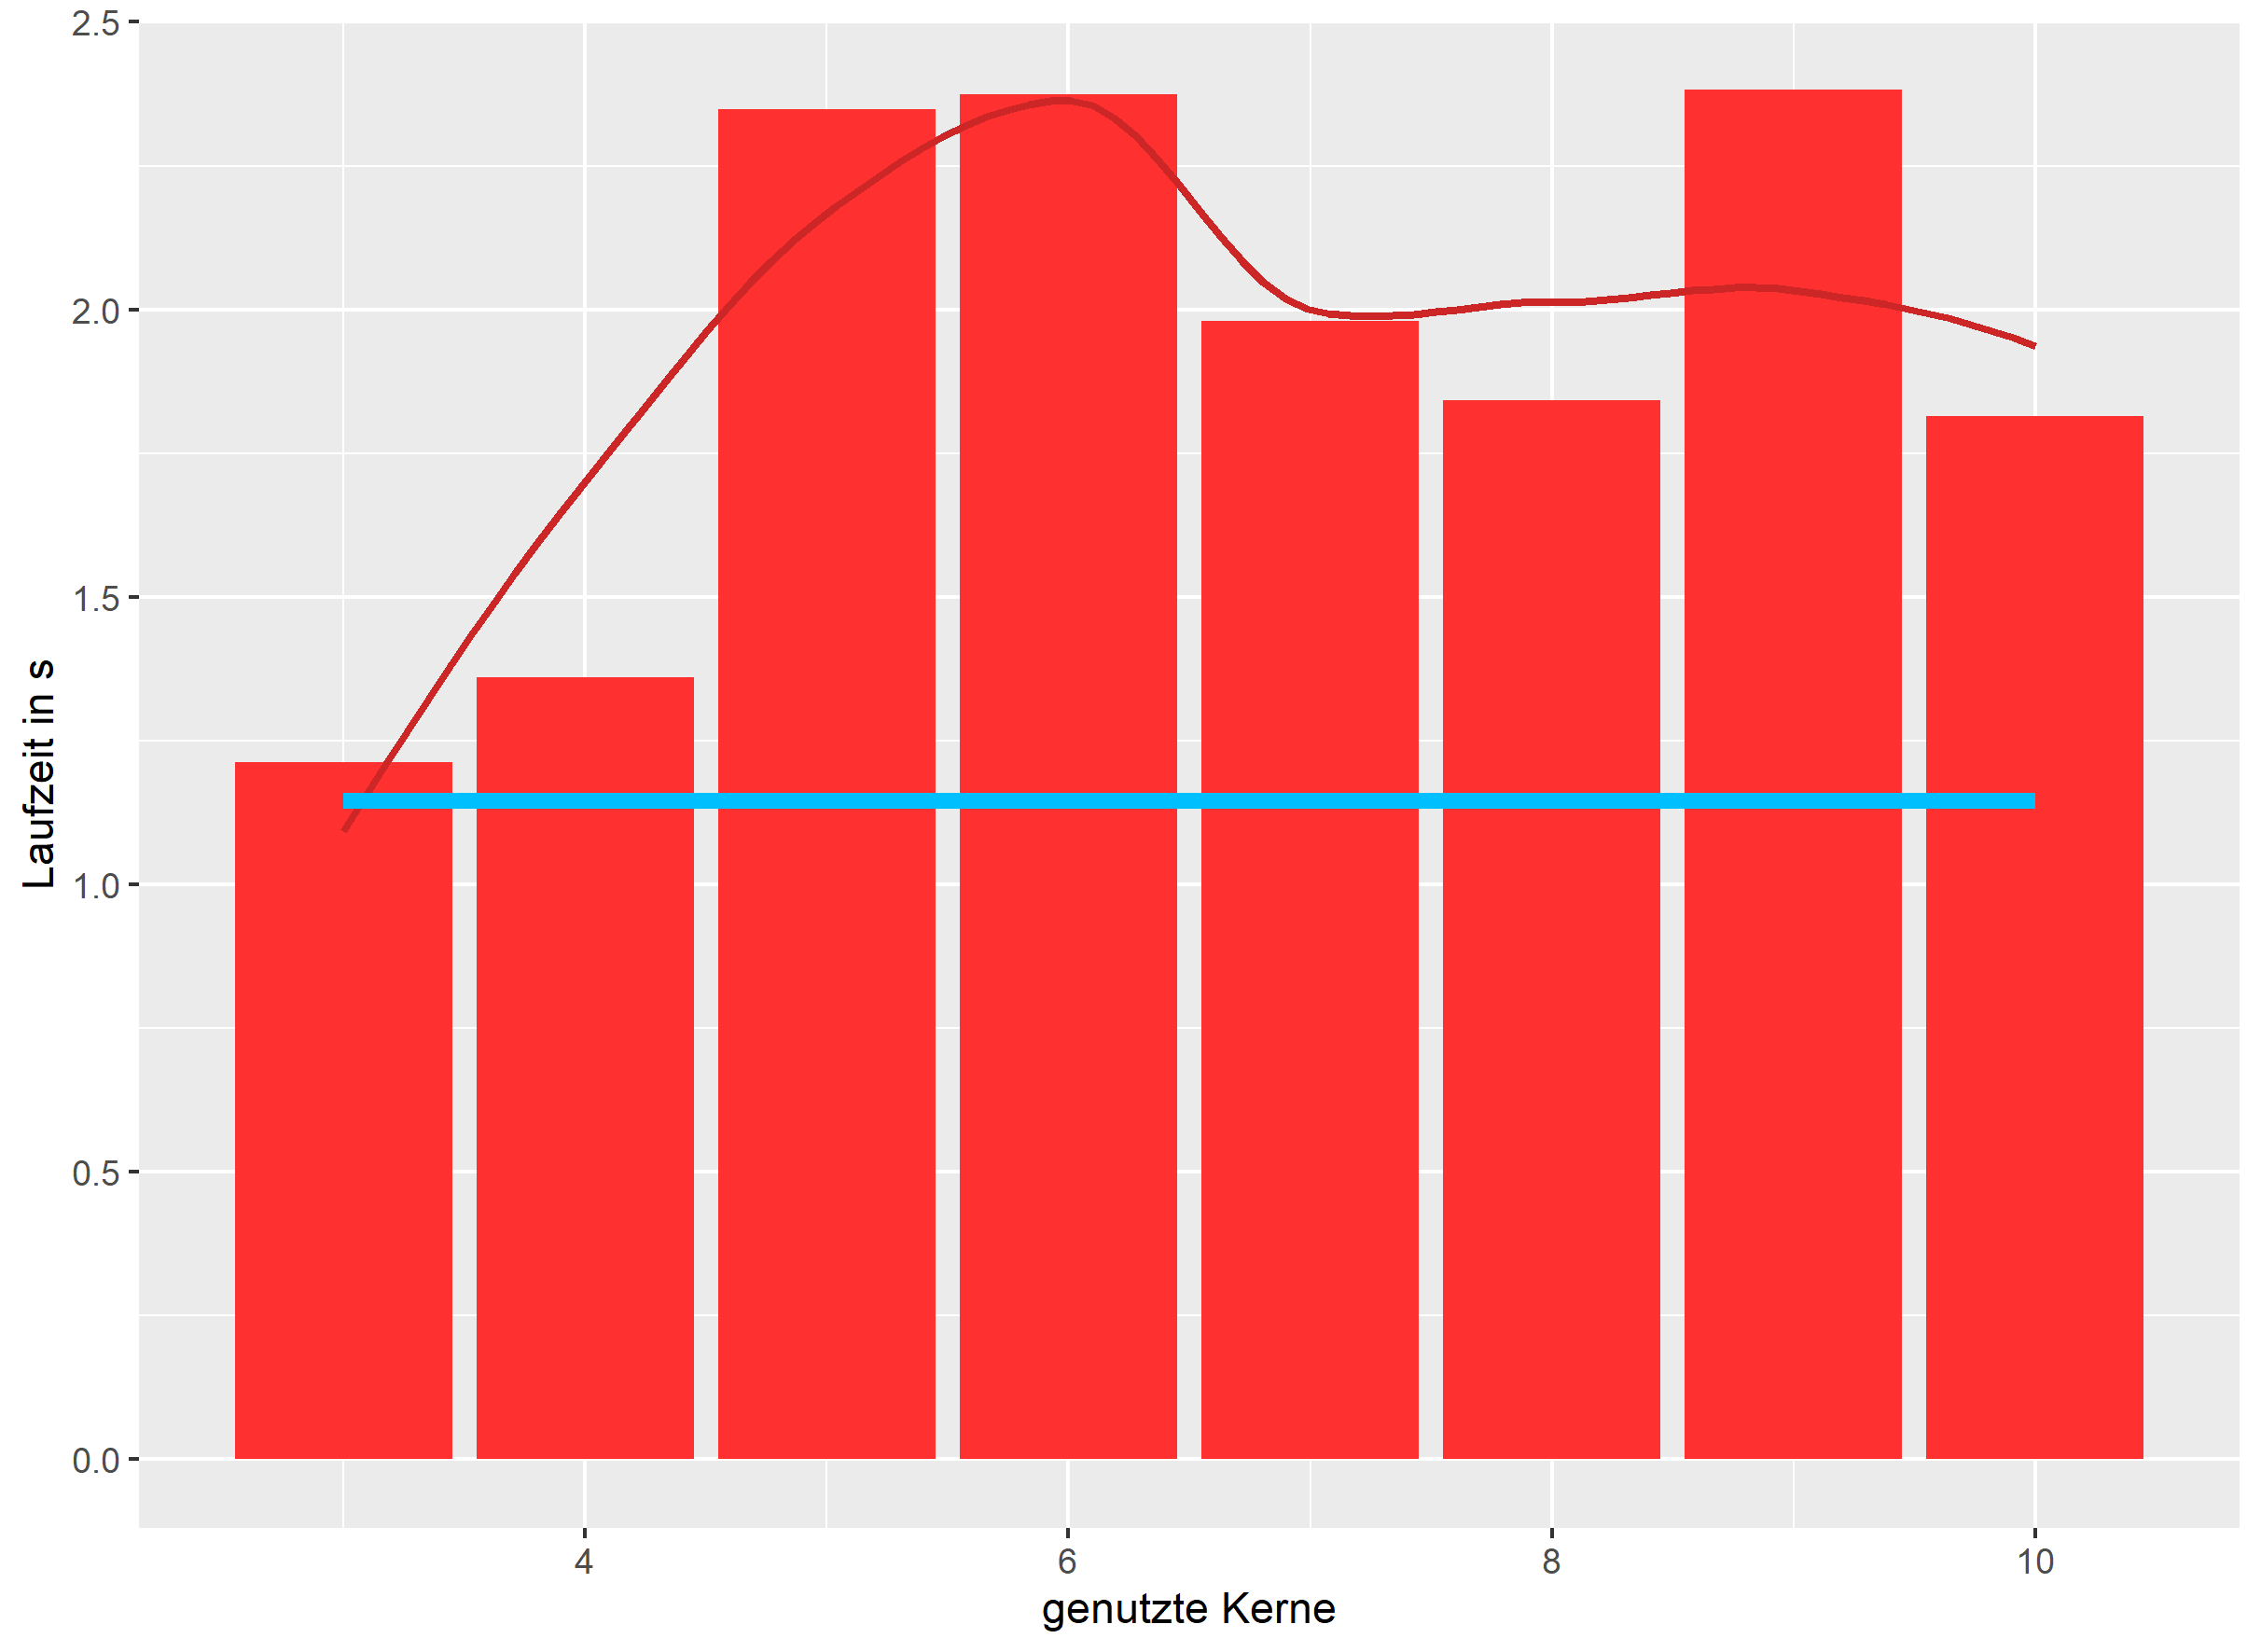
\includegraphics[width=0.45\linewidth]{Bilder/sort_kerne.png}}}
 	\qquad
 	\subfloat[\Fb{roads\_str} nach vielen Attributen\label{img:sortKernMf}]{{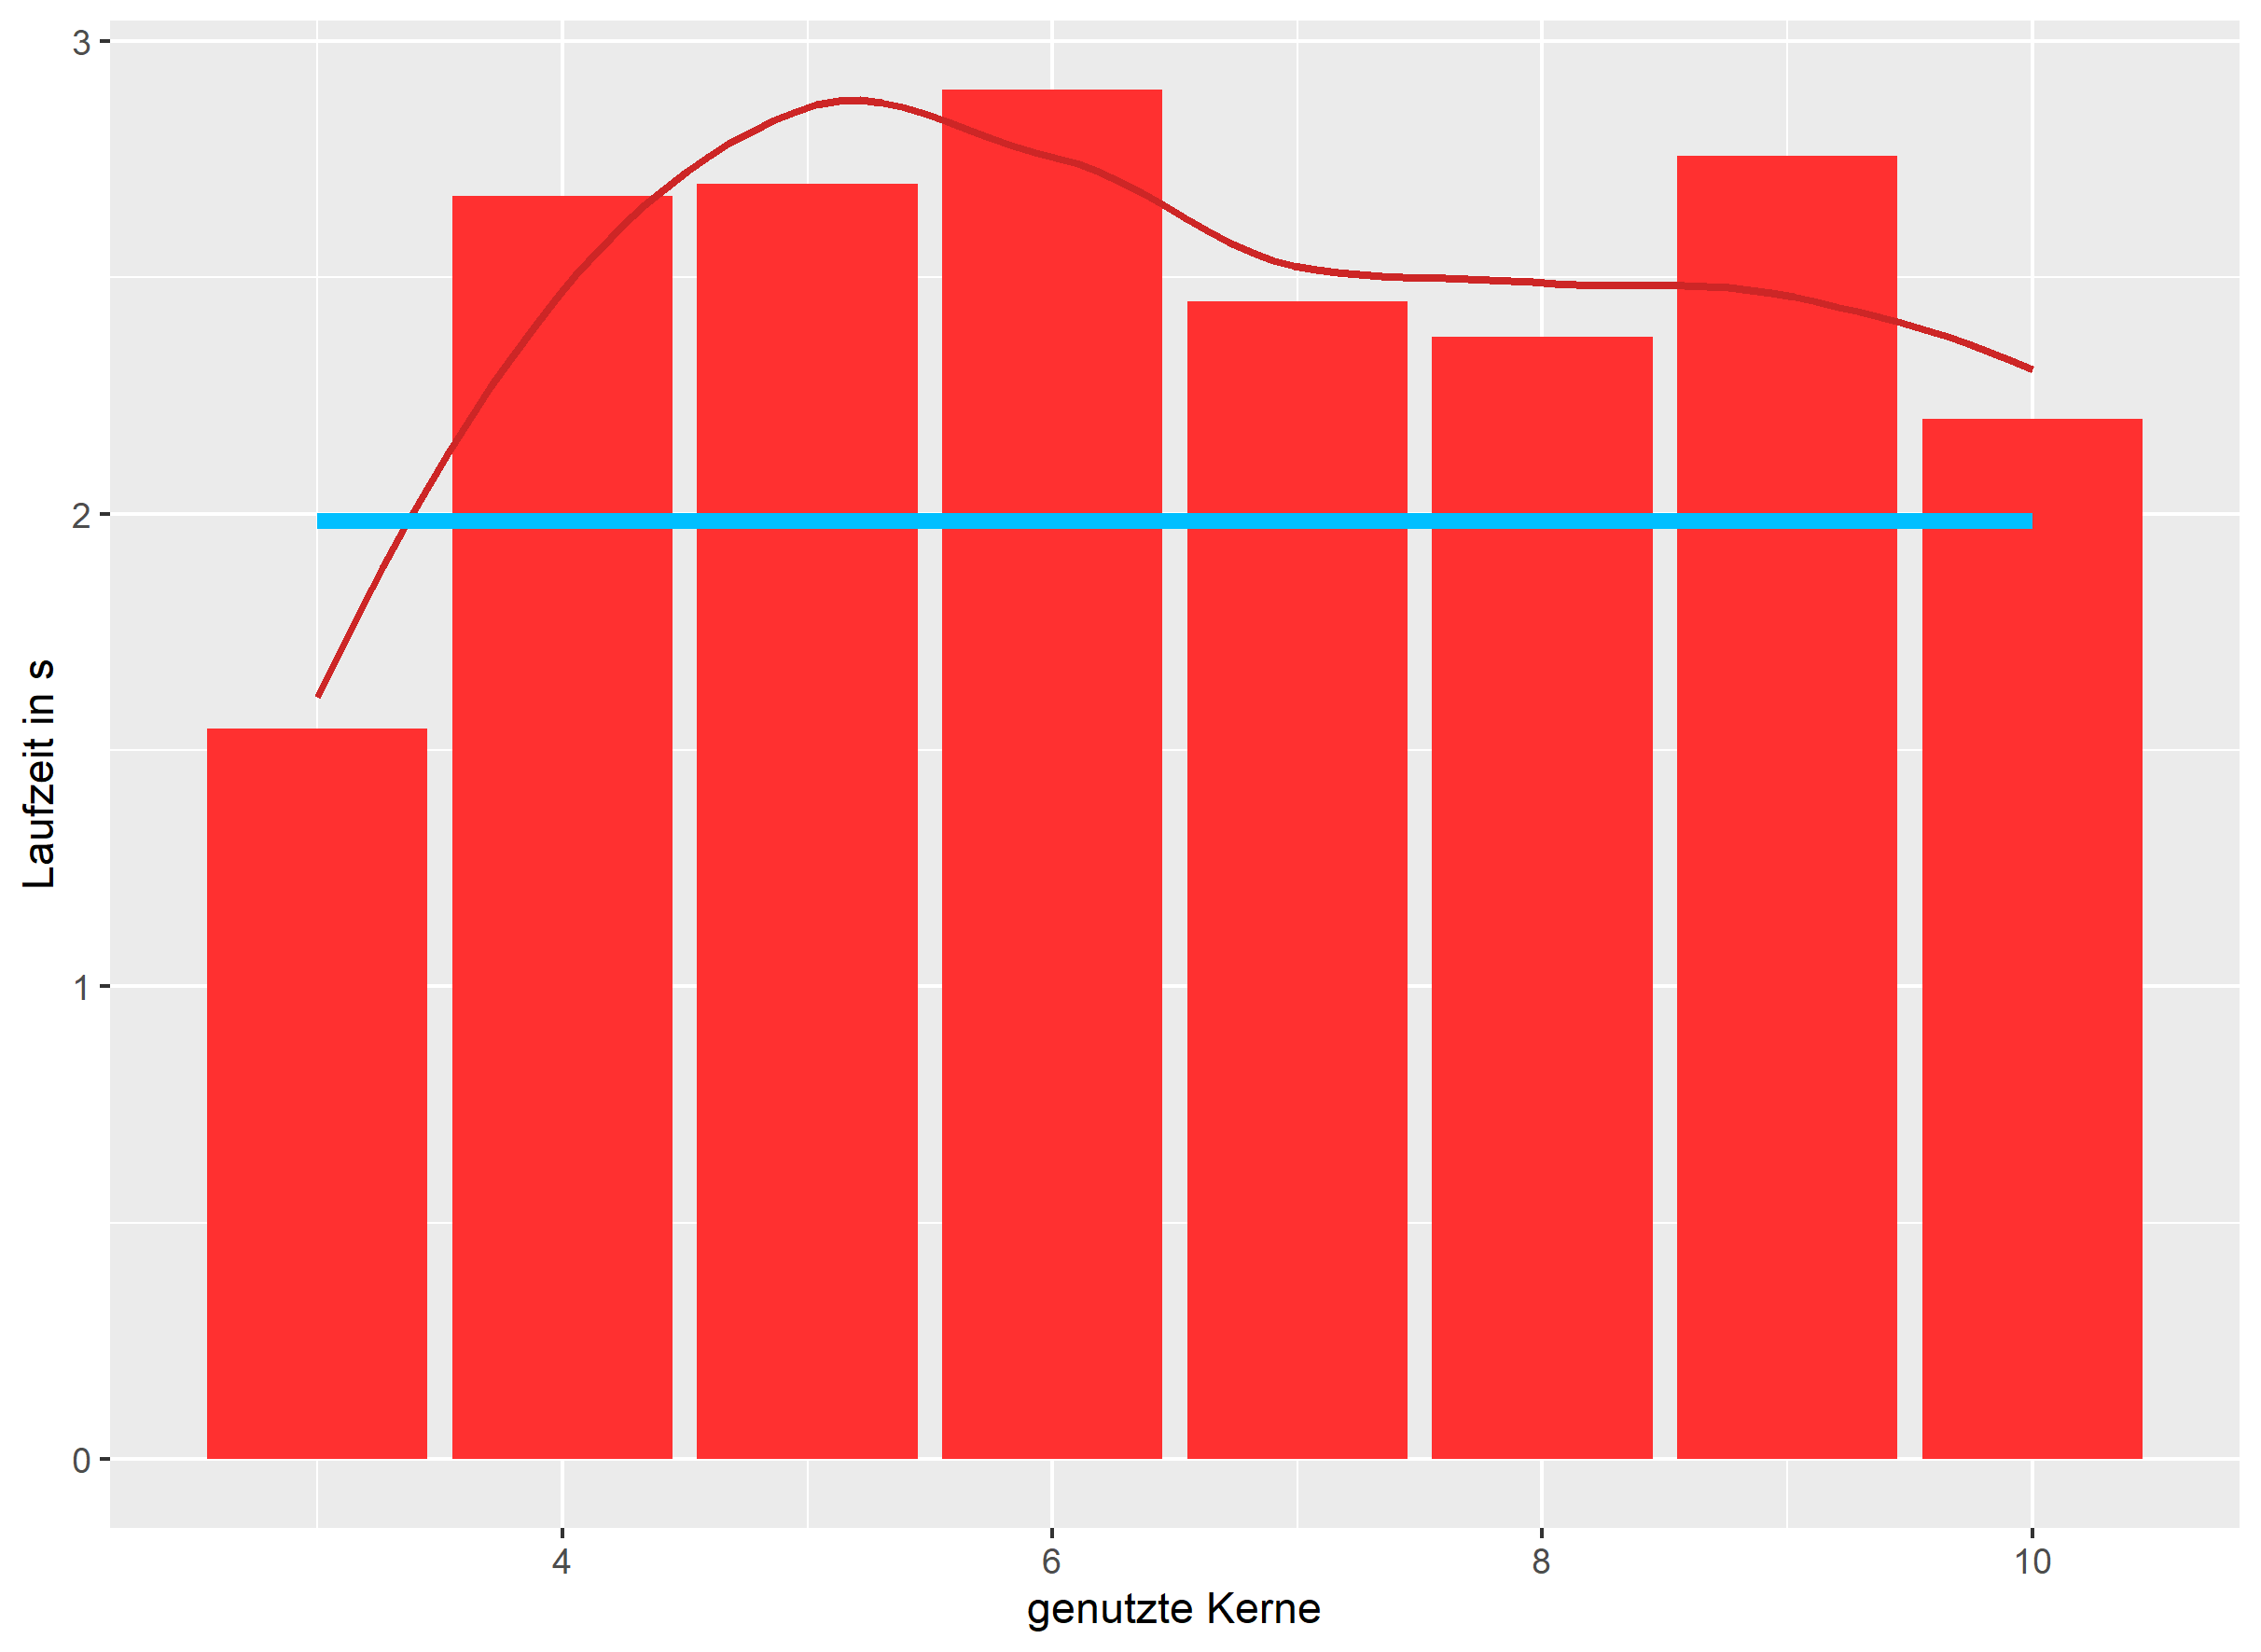
\includegraphics[width=0.45\linewidth]{Bilder/sort_kerne_mf.png}}}
	\caption{Sortierung und Anzahl Kerne. Blaue Gerade: Singlethread-Operator im Vergleich, rote Linie: Glättungskurve.}
	\label{img:sortKernAlg}
\end{figure}

\subsubsection{mThreadedHybridJoin}

Der Multithreading-Hash-Join verfügt über eine komplexe Überlaufstruktur. Zu einem Über"-lauf kommt es bei sehr großen Relationen und vor allem bei einer unausgeglichenen Verteilung über Joinattribute in der R-Relation. Dementsprechend ist es hier für einen Test auf Korrektheit wichtig sicherzustellen, dass in der Gesamtheit der Tests alle Teilbereiche des Codes durchlaufen werden. Um das zu kontrollieren, habe ich für die Testphase in den verschiedenen Methoden bzw. Abzweigen für das Overflow-Handling Ausgaben an die Konsole eingebaut. Getestet wurde ein Selfjoin der \Fb{roads\_str}-Relation (\autoref{list:testjoin}). Da die Relation im Attribut \Fb{Name} einen großen Anteil von Leerstrings hat, haben dementsprechend sehr viele Tupel einen gleichen Hashwert und der Join nähert sich einem kartesischem Produkt an. Selbstverständlich ist für solch einen Join ein Hash-Join keine sinnvolle Wahl, aber die Verteilung innerhalb der Relation stellt sicher, dass die Overflow-Behandlung vollständig durchlaufen wird. Eine Schwierigkeit war es, dass die Join-Operatoren der \Fb{ExtRelationC++}-Algebra nicht stabil sind -- bei großen Relationen mit speicherintensiven Tupeln und sehr großen Ergebnisströmen kam es häufig zu Abstürzen. \autoref{tab:testJoin} zeigt die Ergebnisse dieser Tests. Zusätzlich zu dem durchgeführten Join wird die genutzte Anzahl von Kernen, die Speichereinschränkung und die Verkürzung der Relation mit dem \Fb{head}-Operator angegeben. Um einen Fehler auszuschließen, der bei dem Singlethread-Join auftritt, habe ich einen Hybrid-Hash-Join mit zwei großen Relationen, mit denen die Singlethread-Varianten nicht mehr funktioniert haben, ausgeführt, aber nur die Ausführung ohne Absturz des von mir implementierten Operators dokumentiert. Wenn nicht zwei Joins miteinander über den Gleichheits-Operator verglichen werden, sondern über \Fb{consume} eine neue Relation erzeugt wird, tritt auch bei der Multithread-Variante der Fehler auf, der mehrfach bei den Singlethread-Varianten des Join-Operators aufgetreten ist: Der Operator bricht mit einer Fehlermeldung des Storage-Managers ab, nämlich \Fb{DbEnv: BDB2055 Lock table is out of available lock entries}. Da dieser Fehler aber nicht nur bei meinem Operator, sondern bei den anderen Join-Operatoren in noch viel größerem Maße auftritt, gehe ich von einem Fehler im \Fb{Secondo}-Kern aus.

\begin{minipage}{0.95\textwidth}
	\begin{lstlisting}[caption={Beispiel Testqueries für den Join-Operator.}, label=list:testjoin]
	query (roads_str feed head[5000] {p} roads_str feed {o} mThreadedHybridJoin[NameStr_p, NameStr_o] project[NameStr_o] sortby[NameStr_o]) = (roads_str feed head[5000] {p} roads_str feed {o} sortmergejoin[NameStr_p, NameStr_o] project[NameStr_o] sortby[NameStr_o])
	\end{lstlisting}
\end{minipage}

Zusätzlich habe ich noch Tests mit kleinen und gleichmäßiger verteilten Relationen der Datenbank \Fb{berlintest} durchgeführt, um das Verhalten des Operators bei unterschiedlicher Nutzung an Kernen und Speicher zu untersuchen. 

\begin{table}
	\centering
	\begin{tabular}{|c|c|c|c|c|}
		\hline
		\rowcolor{gray!30}
		Operation & head/memory & Kerne & Overflow-Strukturen & Ergebnis \\ 
		\hline 
		$roads\_str \bowtie roads\_strf$ & 10.000/all & 5 & keine & true \\ 
		\hline 
		$roads\_str \bowtie roads\_str$ & 10.000/2~MB & 5 & keine & true \\ 
		\hline 
		$roads\_str \bowtie roads\_str$ & 20.000/all & 5 & keine & 50.764.348 \\ 
		\hline 
		$pr\_sj\_pr\footnotemark \bowtie pois\_str$ & 30.000/2~MB & 5 & 2 rekursiver Overflow & true \\ 
		\hline 
		$strassen \bowtie Plaetze$ & all/2~MB & 6 & keine  & true \\ 
		\hline
		$strassen \bowtie Plaetze$ & all/all & 3 & keine & true \\ 
		\hline
		$strassen \bowtie Plaetze$ & all/all & 6 & keine & true \\ 
		\hline
		$Orte \bowtie plz$ & all/2~MB & 6 & keine & true \\ 
		\hline
	\end{tabular}
	\caption{\label{tab:testJoin} Korrektheitsnachweis durch Vergleich Singlethread- und Multithread-Version.}
\end{table}

\footnotetext{Die Relation pr\_sj\_pr ist ein Spatial-Join zwischen pois und roads.}

Auf eine Vielzahl unterschiedlicher Relationen und deren Kombinationen wurde bereits getestet. Auch funktioniert der Operator weitestgehend gut mit sehr großen Relationen. Hier ist aber anzumerken, dass, wenn die Gesamtheit der Tupel der R-Relation, deren Joinattribut den gleichen Hashwert hat, nicht in den Hauptspeicher passen, diese nicht vollständig ausgewertet werden, da sonst eine zusätzliche Persistierungsstruktur für einzelne Buckets implementiert werden müsste. In der jetzigen Implementierung werden hier nur die Tupel ignoriert, die nicht mehr in den Hauptspeicher passen. Sinnvoller wäre es sicher, den Operator mit einer Fehlermeldung abbrechen zu lassen.

Problematisch für die Funktionsweise des Operators kann es auch sein, wenn die Eingangsströme entweder ganz leer sind oder so wenige Tupel enthalten, dass eine Partitionierung auf alle Threads nicht möglich ist. Darüber hinaus wird getestet, ob im Type-Mapping Parameter zurückgewiesen werden, die für einen Equi-Join nicht sinnvoll sind. Die vorgenommenen Robustheitstests werden in \autoref{tab:testJoinRobust} dargestellt, wobei die Tests immer bei der Verwendung von sechs Kernen und mit den beiden Relationen \Fb{strassen} sowie \Fb{Plaetze} ausgeführt worden sind, außer wenn es anders vermerkt wurde. Alle durchgeführten Test entsprachen den Erwartungen.

\begin{table}
	\centering
	\begin{tabular}{|p{7.5cm}|p{7.5cm}|}
		\hline
		\rowcolor{gray!30} 
		Test & Ergebnis \\
		\hline
		Eingangsstrom leer & leere Ergebnisrelation \\ 
		\hline
		Eingangsstrom 2 Tupel & 2 TODO manchmal Deadlock \\ 
		\hline
		Joinattribute ohne Übereinstimmungen & TRUE, keine Anlage temporärer Dateien \\
		\hline
		mit 2 Kerne & TRUE  \\
		\hline
		mit 20 Kernen & only works with $\geq$ 3 threads  \\ 
		\hline
		Attribute nicht gleicher Typ & TODOm \\ 
		\hline
		erstes Attribute nicht Teil der Relation & Name\_o is not an attribute of the second stream \\ 
		\hline
		Eingang R kein Strom & first arg is not a tuple stream \\ 
		\hline
		Eingang S kein Strom & second arg is not a tuple stream \\ 
		\hline
		kein Joinattribut & stream(tuple) x stream(tuple) x attr1 x attr2 expected \\ 
		\hline
		3 Joinattribute & stream(tuple) x stream(tuple) x attr1 x attr2 expected \\
		\hline
		3 Eingangsströme &  Syntax error \\
		\hline
	\end{tabular}
	\caption{\label{tab:testJoinRobust}Robustheit Merge-Sort.}
\end{table}

Die Effizienz des Operators wird hier nur für Joins von Relationen untersucht, deren Verteilung den Einsatz eines Hash-Joins sinnvoll erscheinen lässt. Dies bedeutet vor allem, dass in den Relationen wenig Duplikate in den Joinattributen vorkommen, die einerseits zu einer sehr großen Anzahl von Ergebnistupeln führen und andererseits alle den gleichen Hashwert haben, also zu ungleich gefüllten Buckets führen. Dies würde zu Performanceproblemen für einen Hash-Join führen, der nur effizient arbeitet, wenn die Tupel gleichmäßig auf die Buckets verteilt werden. Vergleichen wird der \Fb{mThreadedHybridJoin} mit seiner Singlethread-Variante, dem \Fb{hybridhashjoin} mit 100 und 1000 Buckets unter Nutzung einer verschiedenen Anzahl von Kernen. \autoref{img:joinKern} zeigt die Laufzeitanalyse eines Selfjoins der Relation \Fb{roads\_str} -- die verwendete Relation hat 44.684 Tupel und wegen einer Duplikate in den Straßennamen ergibt der Join einen 841.036 Tupel großen Strom als Ergebnis. \autoref{img:joinKernBe} zeigt das Laufzeitverhalten bei zwei Relationen der Datenbank \Fb{berlintest}. Bei $Strassen \bowtie Plaetze$ ist die R-Relation wesentlich größer als die S-Relation und liefert nur 15 Tupel als Ergebnis, bei $Orte \bowtie PLZ$ ist die R-Relation deutlich kleiner und der Join liefert 10.052 Tupel als Ergebnis.

Die Multithread-Variante ist in allen Fällen nicht so effizient wie die Singlethread-Variante. Allerdings können aus dem Verhalten bei einer unterschiedlichen Zahl genutzter Kerne der verschiedenen Joins Rückschlüsse darauf gezogen werden, wo genau die Performanceprobleme des Operators liegen. Im Detail werde ich dies unter Berücksichtigung weiterer Experimente im \autoref{exp:hash} diskutieren. Am besten im Vergleich zur Singlethread-Variante schneidet der Operator ab, wenn die R-Relation sehr klein ist. Die Größe der S-Relation dagegen scheint wenig Einfluss zu haben, da sie beim Selfjoin und bei $Orte \bowtie PLZ$ ungefähr gleichgroß ist. Also liegt vor allem ein Problem beim Aufbau der Hash-Tabellen vor. Einerseits benötigt meine Implementierung einen Scan über die R-Relation mehr als die Singlethread-Variante für die Partitionierung. Andererseits wird in jedem Thread nur das erste Bucket direkt auf eine Hashtabelle verteilt, die anderen entweder im Speicher oder in einem Tupelfile zwischengespeichert. Dieser Ansatz wurde so gewählt, da er einfacher zu implementieren ist, weil Persistierungsstrukturen genauso behandelt werden können wie speicherinterne Strukturen. Aber hier wäre es sicher sinnvoll, einen Ansatz zu wählen, der, sofern genug Hauptspeicher zur Verfügung steht, direkt Hashtabellen berechnet auch für die Buckets, die nicht im ersten Anlauf behandelt werden. 

\begin{figure}
	\centering
	\subfloat[Selfjoin von \Fb{roads\_str}.\label{img:joinKern}]{\raisebox{1.65cm}{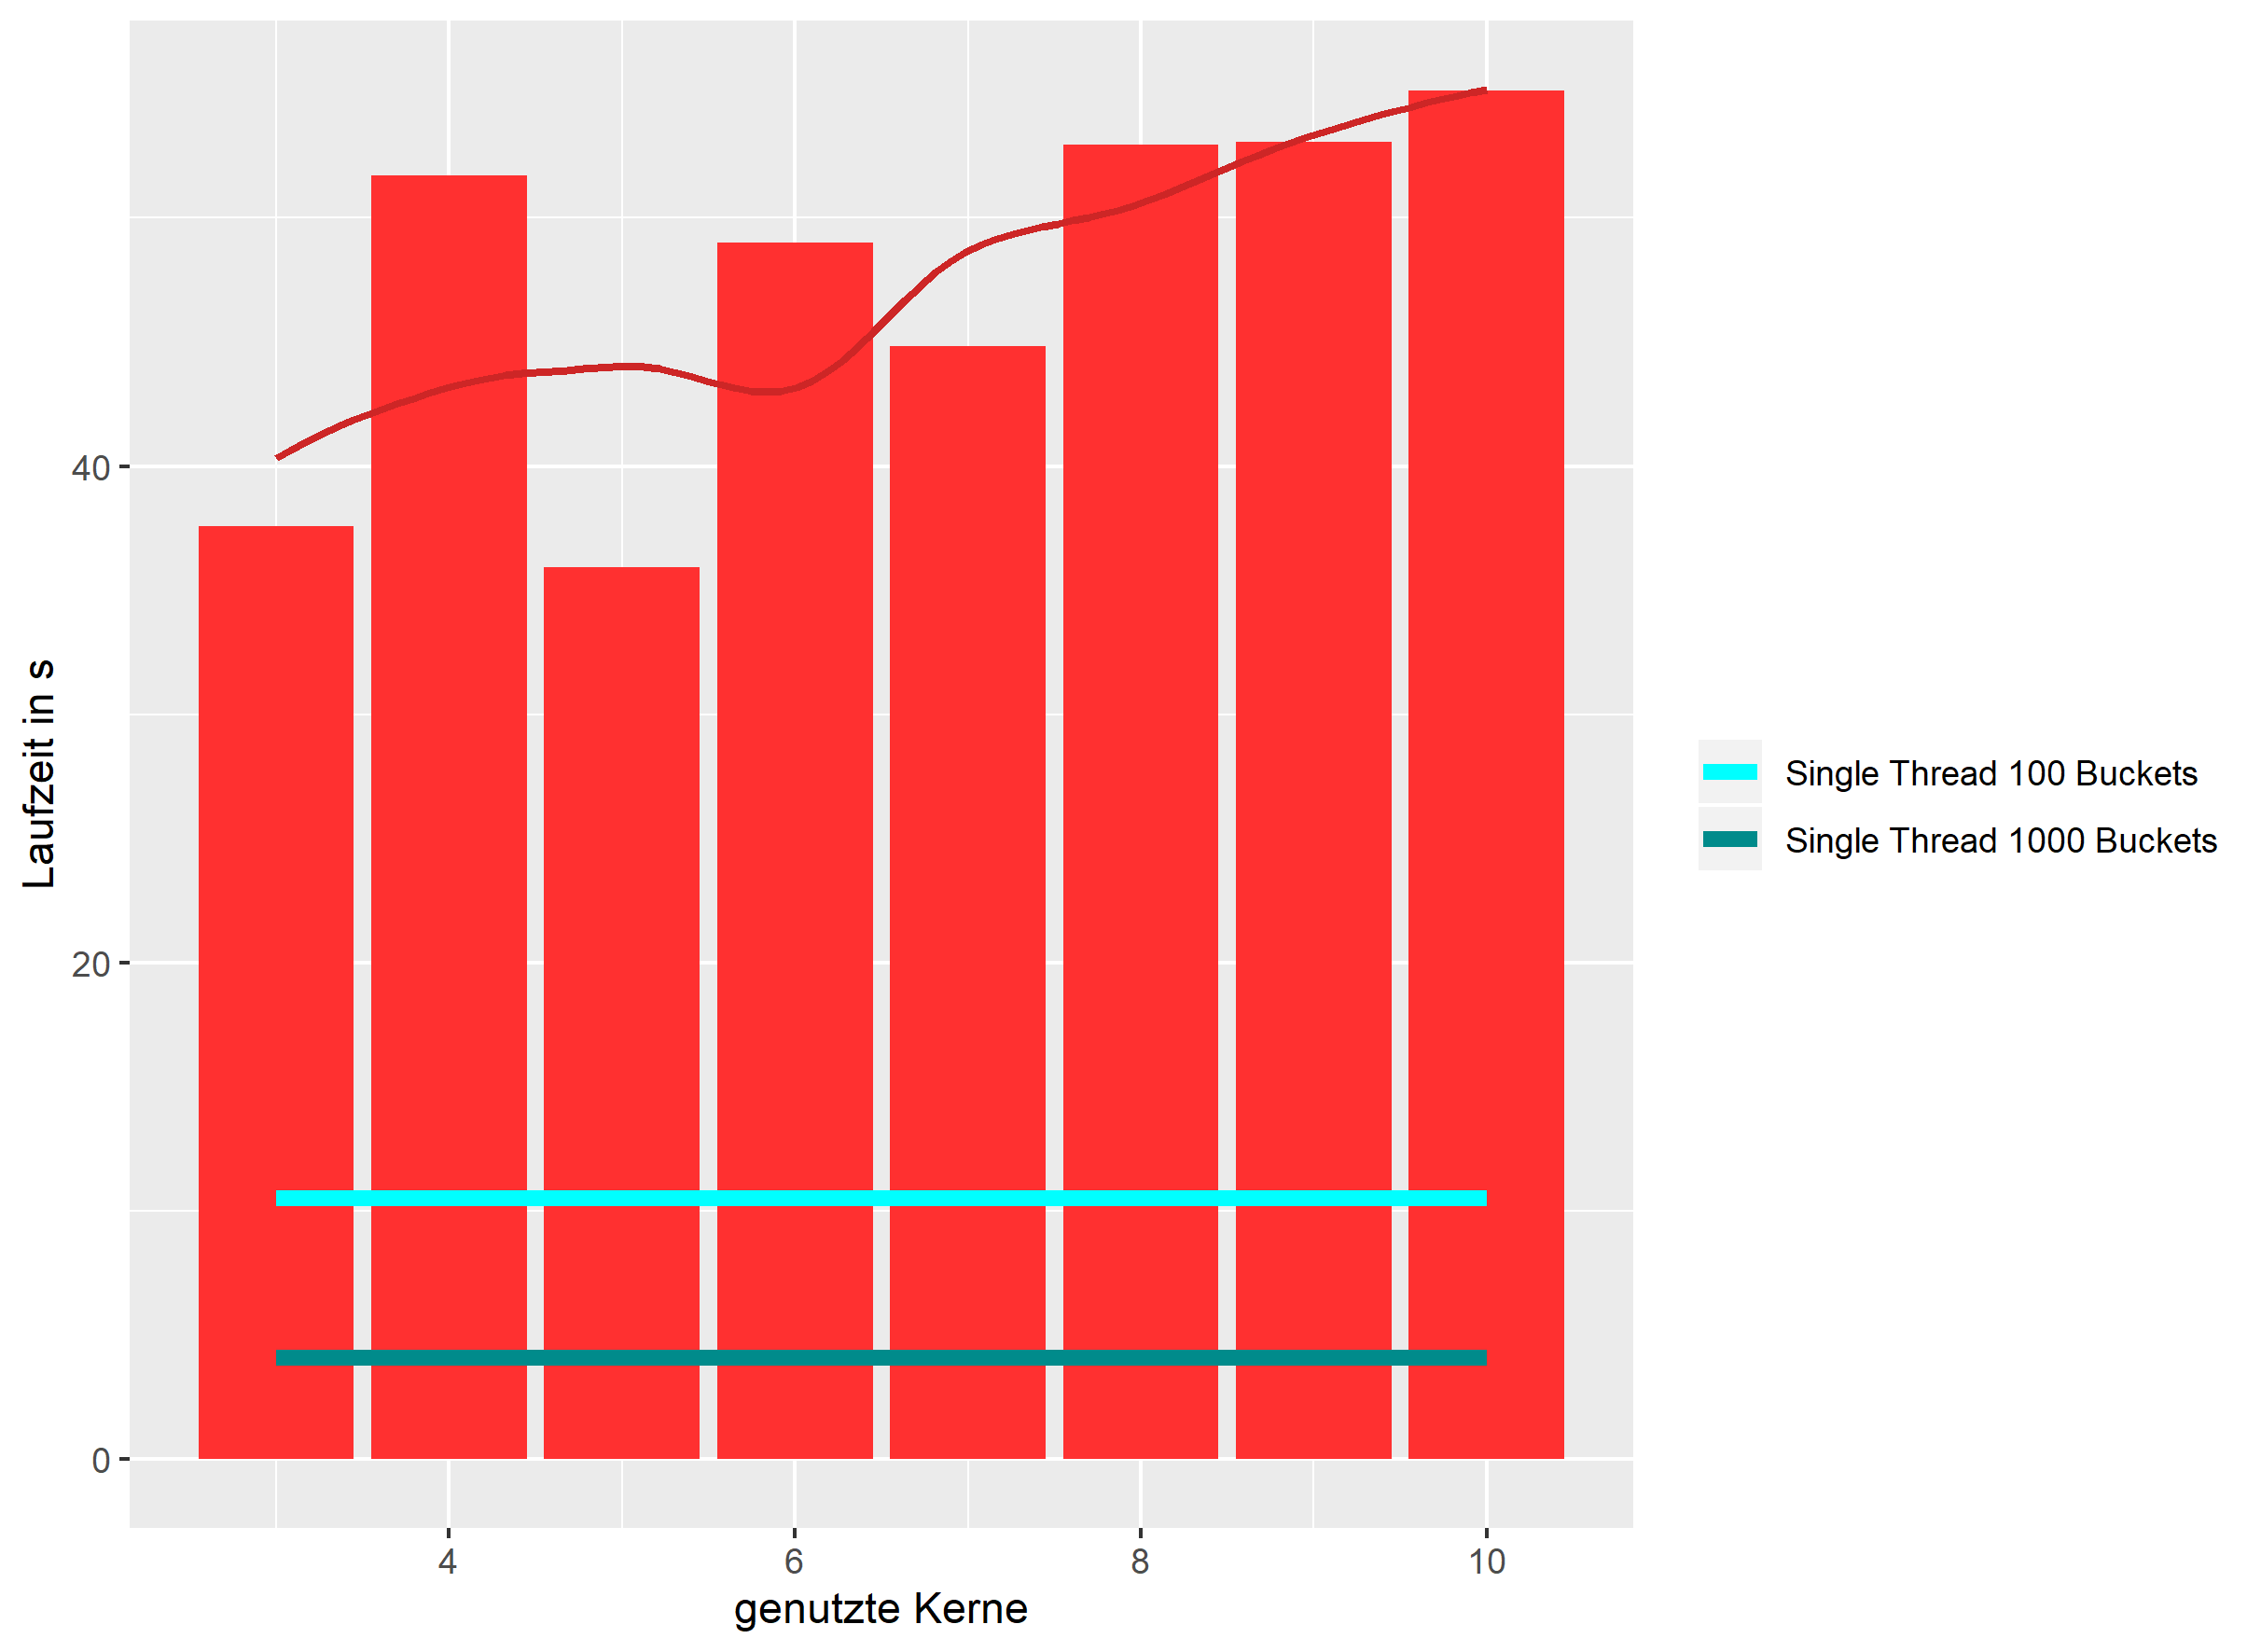
\includegraphics[width=0.3\textwidth]{Bilder/join_kerne_self.png}}}
	\qquad
	\subfloat[Relationen aus \Fb{berlintest}.\label{img:joinKernBe}]{{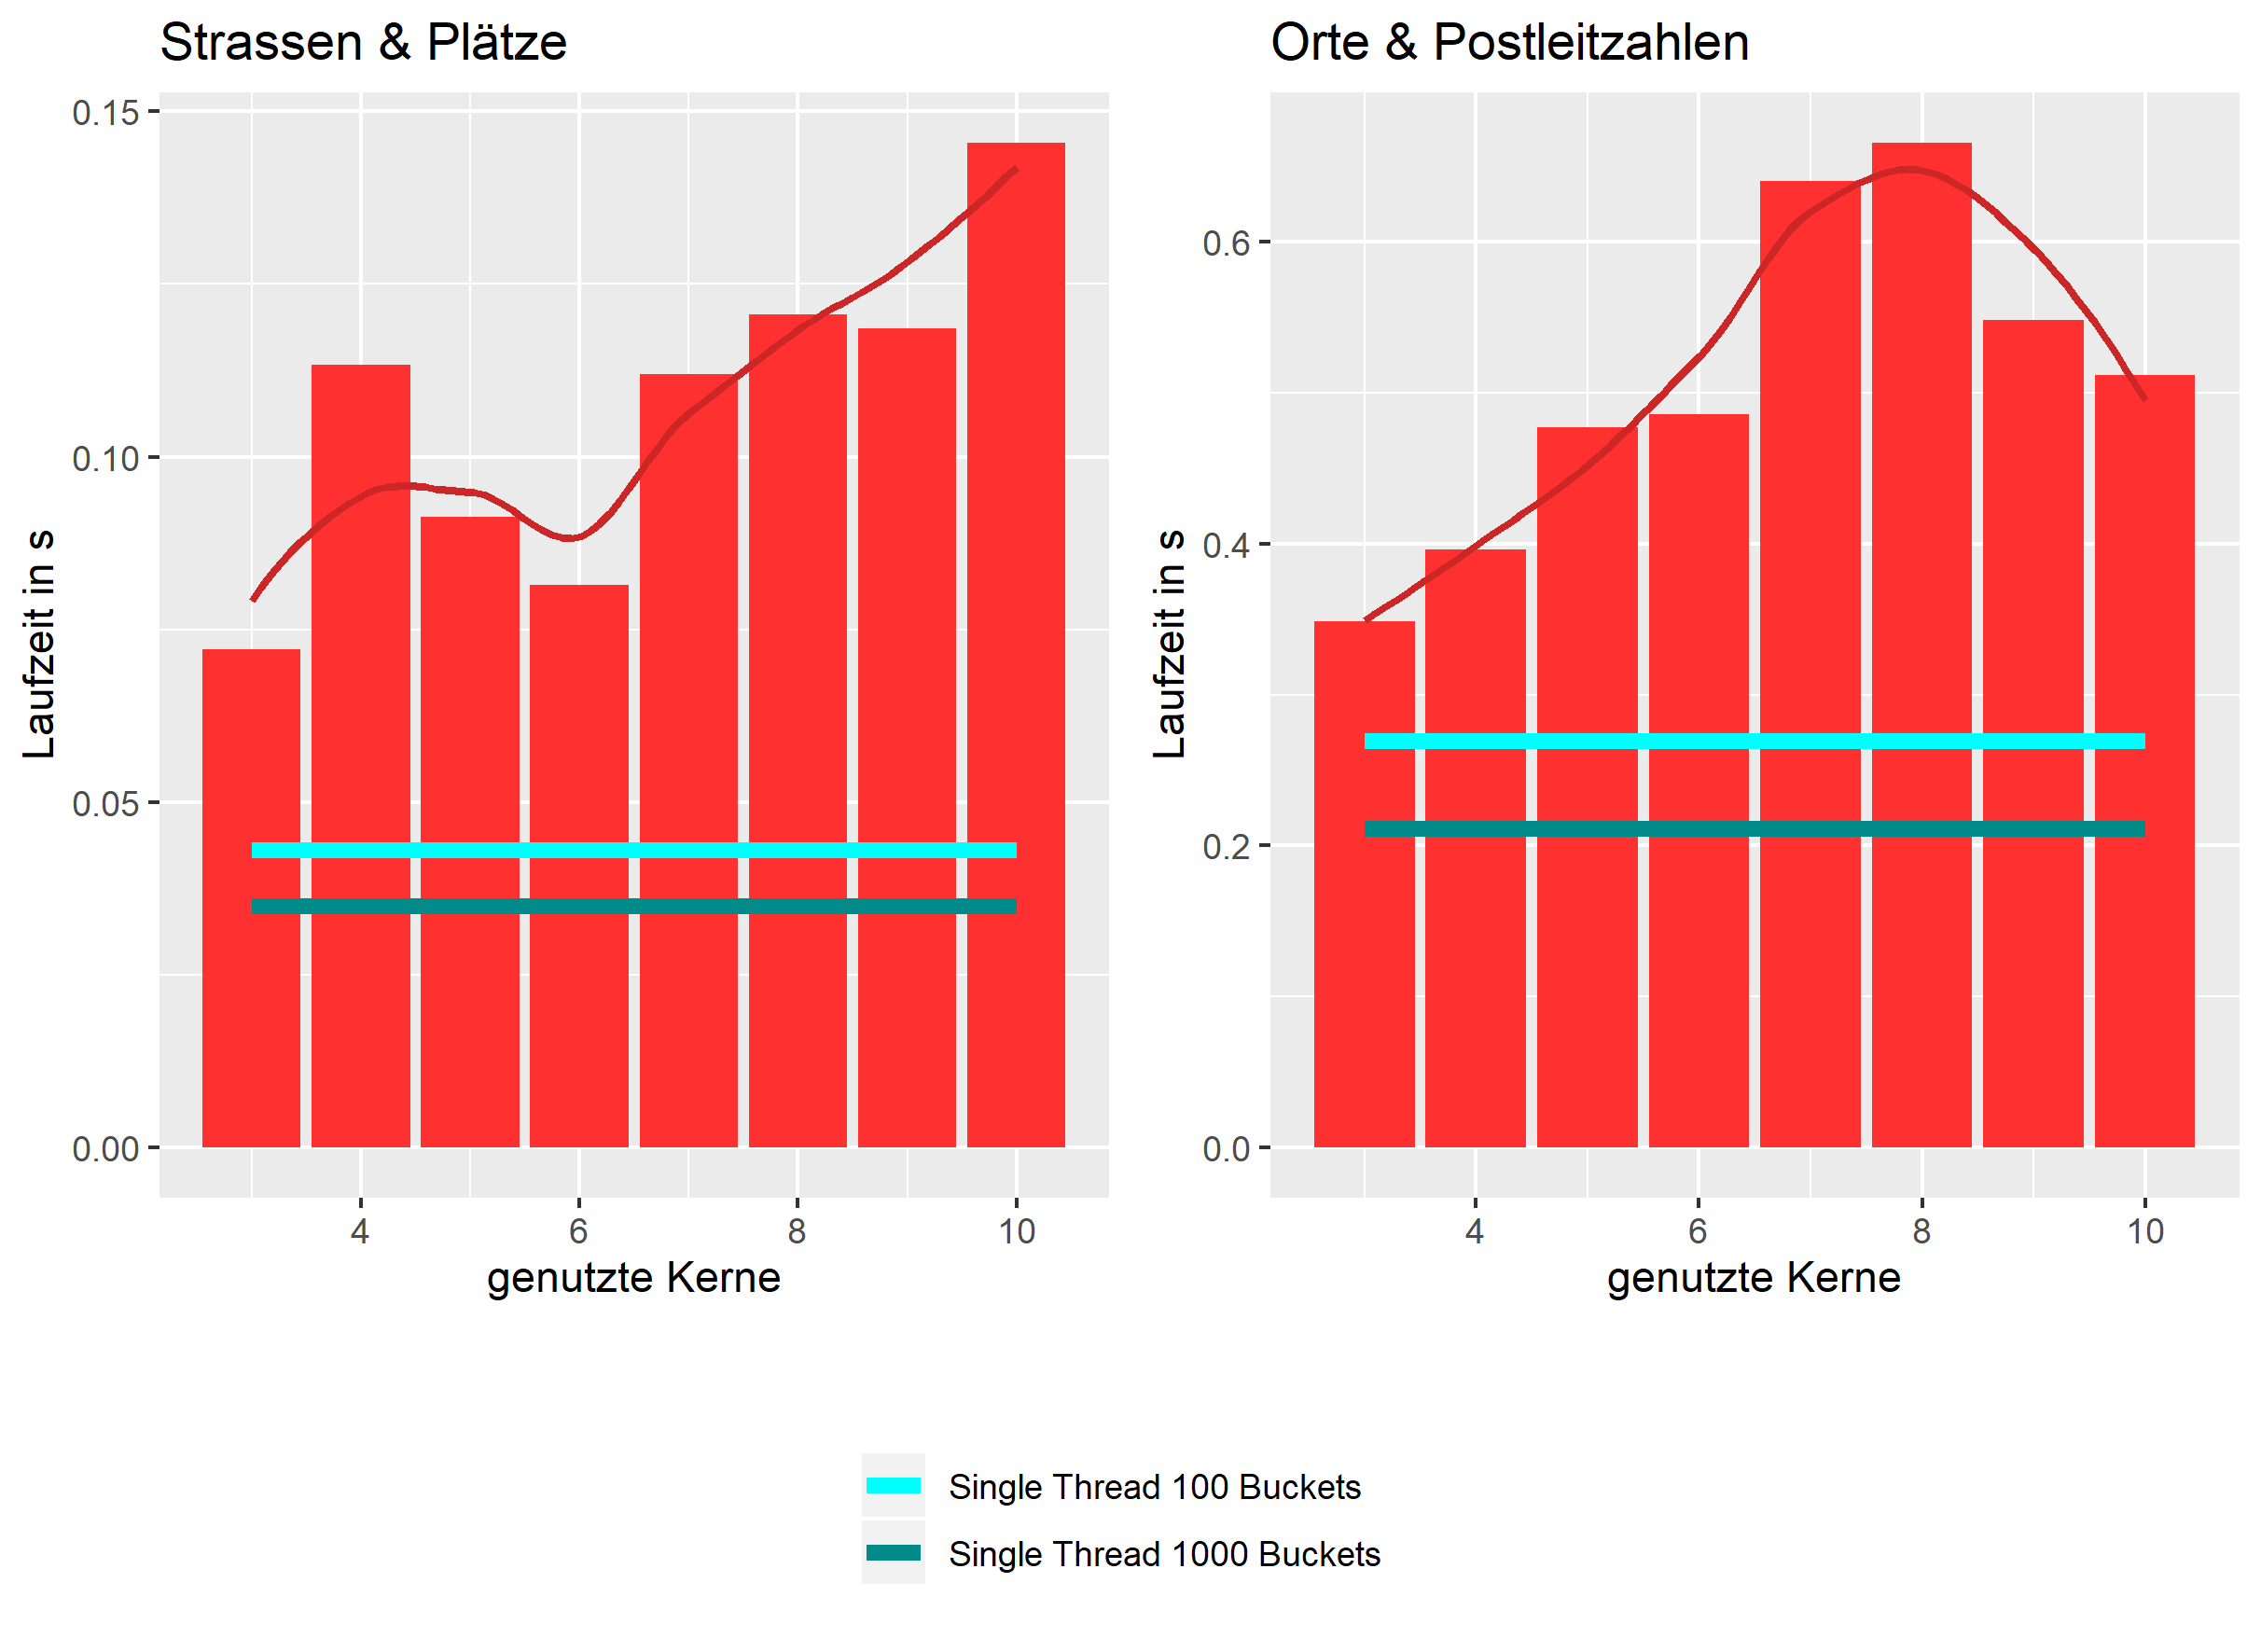
\includegraphics[width=0.6\textwidth]{Bilder/join_kerne_be.png}}}
	\caption{Laufzeitverhalten nach Kernen des Hybrid-Hash-Join.}
	\label{img:joinKernAllg}
\end{figure}

Aufwändig wird die Berechnung der Joins vor allem, wenn viele Tupel in das gleiche Bucket eingefügt werden, also den gleichen Hashwert haben. Wenn dadurch die Verteilung zwischen den Threads insbesondere für die aufwändigen Berechnungen sehr ungleich wird, verliert der Multithread-Operator Vorteile gegenüber dem Singlethread-Version. Beide Joins aus \autoref{img:joinKernBe} zeigen ein Verhältnis aus vergangener Zeit und CPU-Zeit \footnote{ca. 0,65 bei drei Threads, sinkend mit Anzahl genutzter Kerne.}, welches auf eine stärkere Parallelisierung als beim Join in \autoref{img:joinKern} \footnote{ca. 0,8, fast konstant bleibend bezüglich Anzahl der Kerne} hinweist. Für das schlechtere Laufzeitverhalten des Selfjoins gegenüber den beiden anderen Joins gäbe es zwei mögliche Erklärungen: I/O-Zugriffe, die nicht parallelisiert werden können oder eine ungünstige Verteilung auf die Hashtabellen und Threads.

Das Laufzeitverhalten der beiden Joins insgesamt kleinerer Relationen der Datenbank \Fb{berlintest} verschlechtert sich deutlich stärker mit der Anzahl genutzter Kerne, als dies bei großen Relationen wie \Fb{roads\_str} der Fall ist. Grund dürfte vor allem sein, dass wegen der geringen Relationsgröße die Anzahl der Tupel pro Threads zu klein wird für eine sinnvolle Ausführung eines Hybrid-Hash-Joins.

\subsubsection{mThreadedSpatialJoin}

\begin{figure}
	\centering
	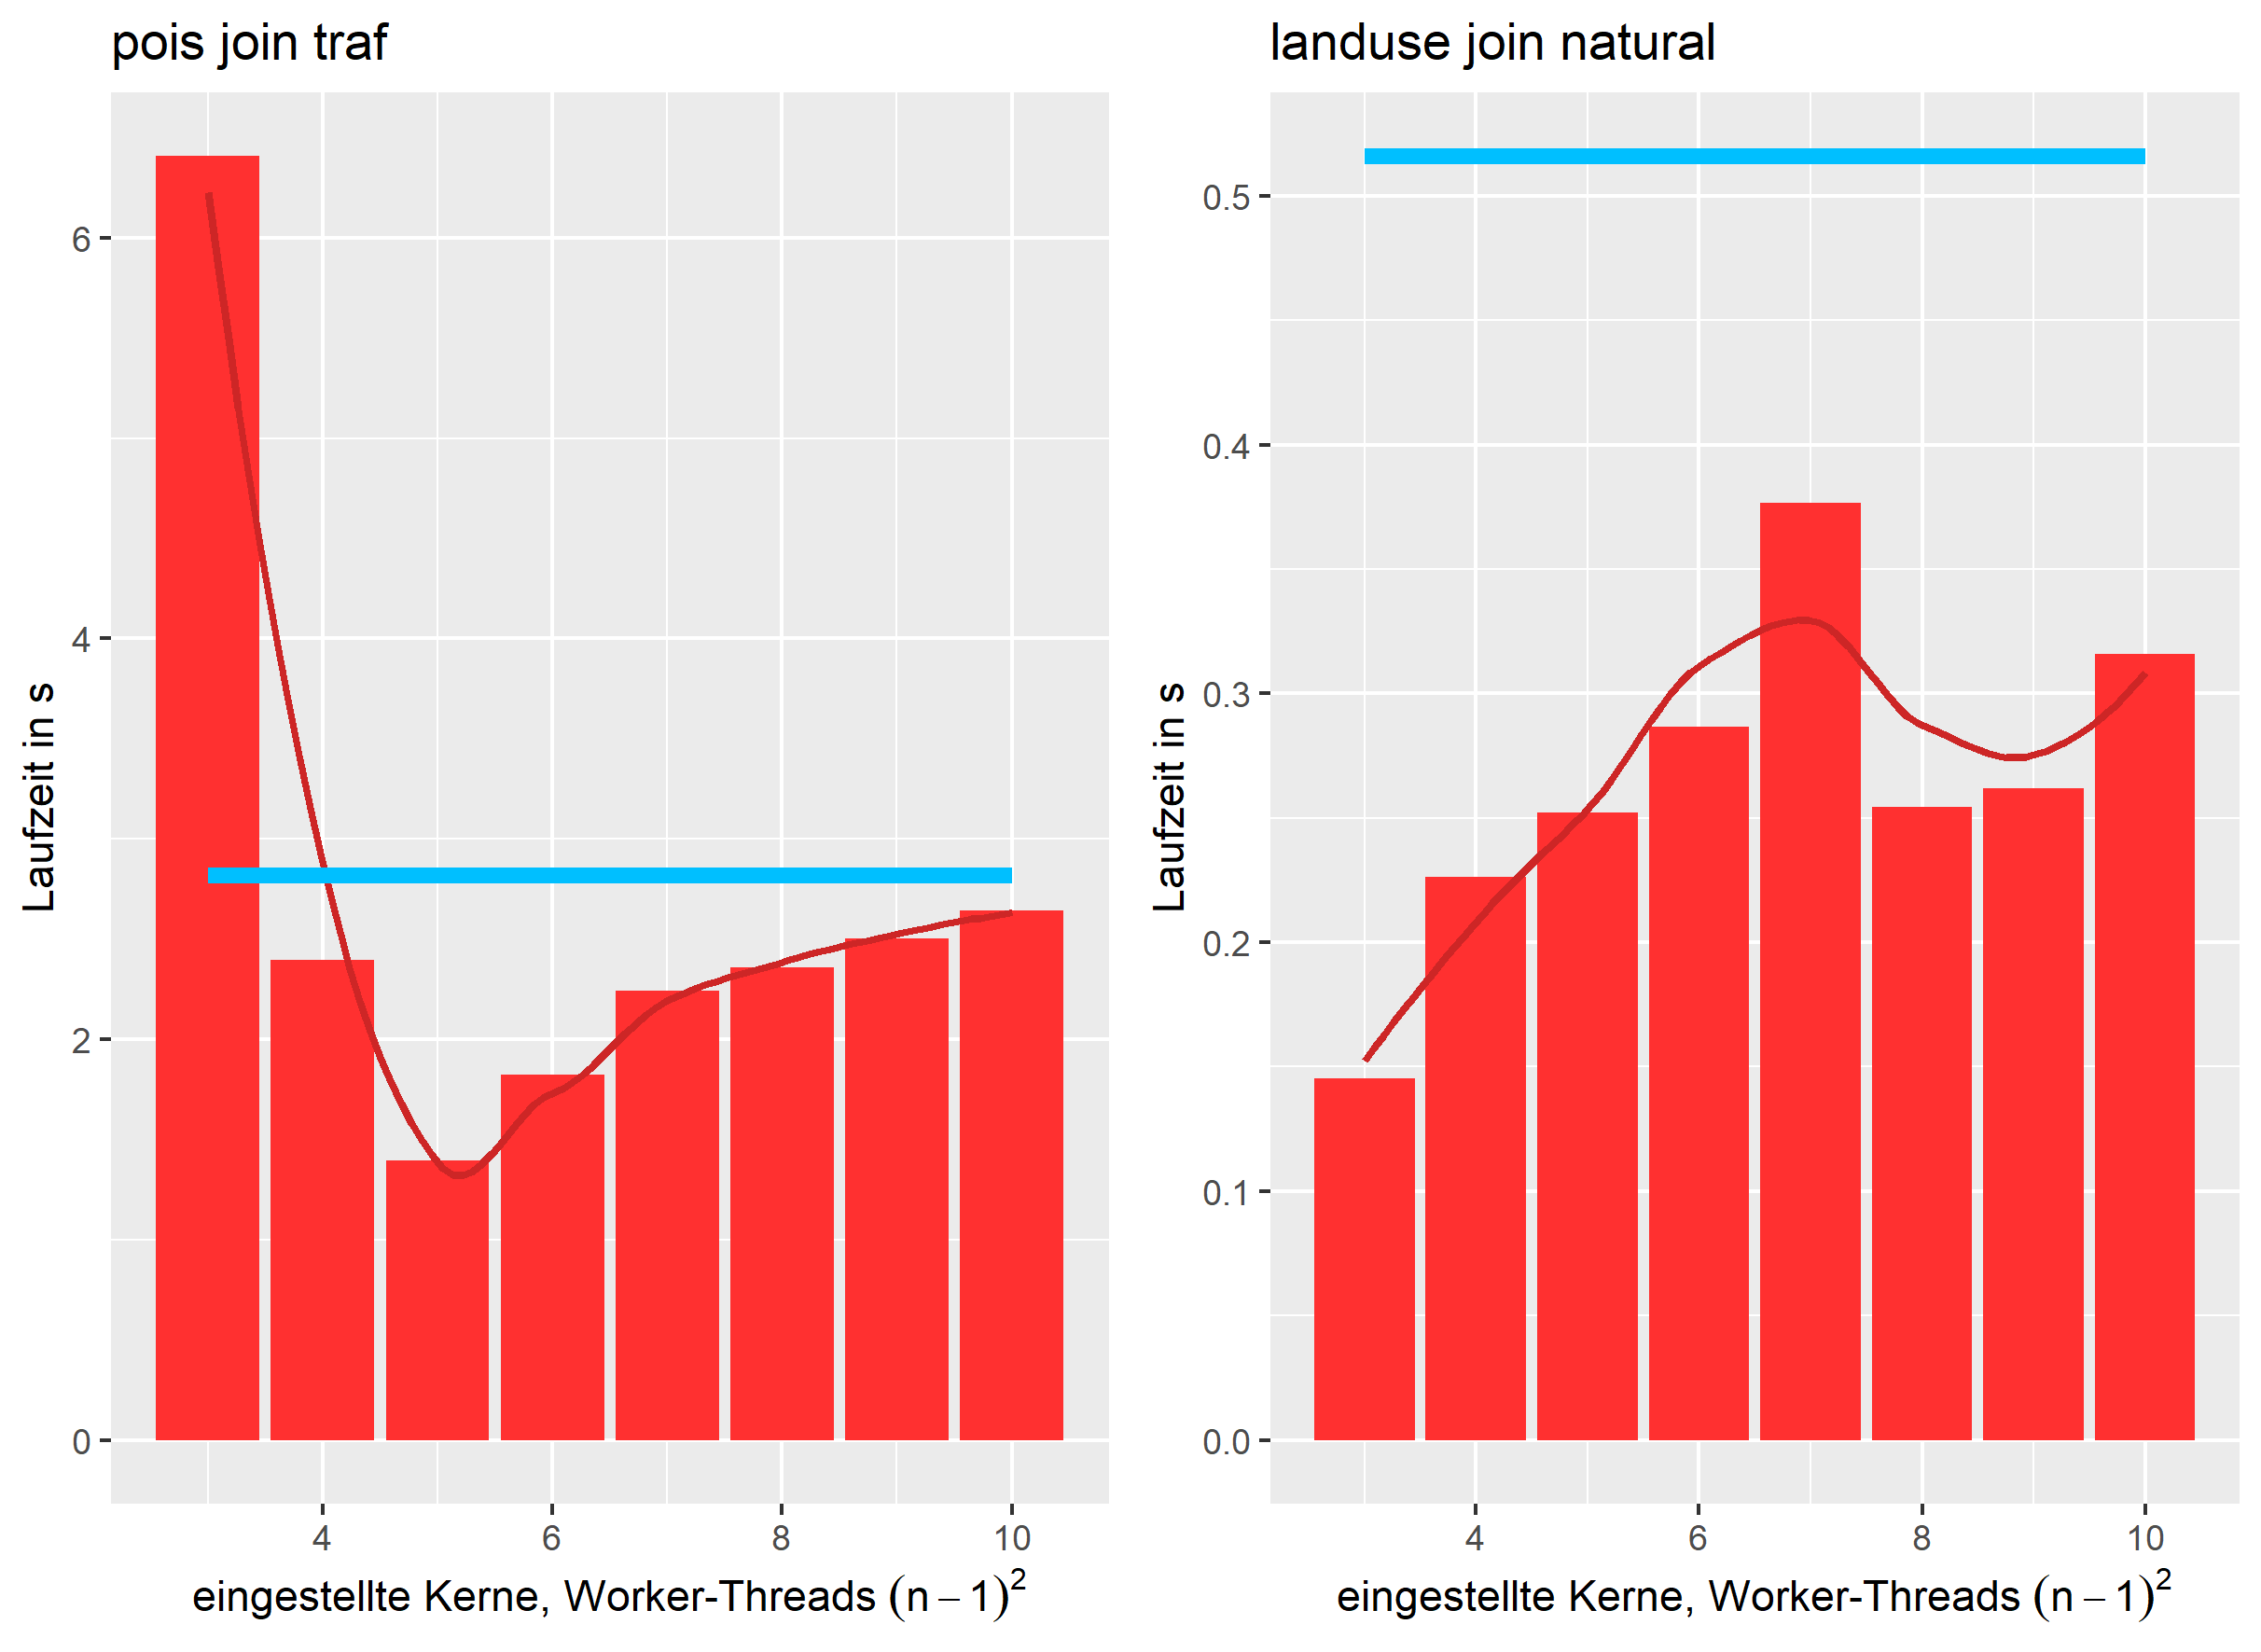
\includegraphics[width=0.60\textwidth]{Bilder/sj_kerne.png}
	\caption{Laufzeit zweier unterschiedlicher Spatial-Joins im Vergleich mit der Single-Thread-Variante (blaue Linie).}
	\label{img:sjKern}
\end{figure}

Der Selbsttest des Spatial-Join-Operator zeigt mit der Option \Fb{-{}-valgrindlc} auch bei großen Relationen kein Speicherleck.

Zeile 1 in \autoref{list:testspatialjoin}) zeigt den Aufruf des Operators. Der Test auf Korrektheit muss sicherstellen, dass jeder Programmteil des Operators durchlaufen wird. Deswegen wird mit unterschiedlich großen Relationen und einer Begrenzung des Arbeitsspeichers getestet. Zusätzlich habe ich mir die Anzahl der Iterationen über die S-Relation ausgeben lassen, um zu beobachten, inwieweit Teile von Relationen ausgelagert wurden. Duplikate können nur bei Attributen auftreten, die eine räumliche Ausdehnung haben (also nicht bei Punkten). Zum Test der Duplikatseliminierung wird deswegen mit Attributen des Typs \Fb{Region} und vielen Kernen -- und damit vielen Partitionen -- getestet, um Duplikate wahrscheinlich zu machen. Verglichen werden die Ergebnisse mit dem Singlethread-Spatial-Join (Zeile 2 in \autoref{list:testspatialjoin}). Da eine gleiche Sortierung der Ergebnisrelation nicht garantiert werden kann, wird vor dem Vergleich die Ergebnisrelation auf die beiden Attribute \Fb{Name} der Eingangsrelationen projiziert und sortiert. Für den Test der Korrektheit der Option, die eine Vergrößerung der \Fb{MBB} ermöglicht, musste als Vergleich der \Fb{symmjoin}-Operator genutzt werden, dessen Eingangsstrom um die vergrößerte \Fb{MBB} ergänzt wurde (Zeile 3 in \autoref{list:testspatialjoin}). \autoref{tab:testSpatial} gibt eine Übersicht über die gemachten Tests, die alle fehlerfrei verliefen. In der Spalte \Fb{speicherintern} ist die Anzahl der Iterationen dargestellt. 

\begin{minipage}{0.95\textwidth}
	\begin{lstlisting}[caption={Beispiel Testqueries für den Spatial-Join-Operator ohne \Fb{project} und \Fb{sortby}.}, label=list:testspatialjoin]
	query roads feed{o} pois feed{p} mThreadedSpatialJoin[Geometry_o, Geometry_p, 0.0]
	query roads feed{o} pois feed{p} spatialjoin[Geometry_o, Geometry_p]
	query roads feed extend[B:enlargeRect(bbox(.Geometry),1.0,1.0)]{o} pois feed extend[B:bbox(.Geometry)] {p} symmjoin[.B_o intersects ..B_p]
	\end{lstlisting}
\end{minipage}


\begin{table}
	\centering
	\begin{tabular}{|c|c|c|c|c|}
		\hline
		\rowcolor{gray!30} 
		Relationen & Threads & speicherintern & Typ Joinattribute & Tupel Ergebnisrelation \\ 
		\hline 
		$pois \bowtie traf$ & 3 & ja & Point \& Point & true \\ 
		\hline 
		$pois \bowtie roads$ & 3 & ja & Point \& Line & true \\ 
		\hline
		$pois \bowtie places$ & 3 & ja & Point \& Region & true \\ 
		\hline
		$roads \bowtie waterways$ & 3 & ja & Line \& Line & true \\ 
		\hline
		$roads \bowtie landuse$ & 3 & ja & Line \& Region & true \\ 
		\hline
		$landuse \bowtie natural$ & 3 & ja & Region \& Region & true \\ 
		\hline
		$roads \bowtie natural$ & 3 & ja & Line \& Region & true \\ 
		\hline
		$roads \bowtie natural$ & 6 & ja & Line \& Region & true \\ 
		\hline
		$roads \bowtie natural$ & 6 & nein & Line \& Region & true \\ 
		\hline
		$roads \bowtie natural$ & 6 & nein & Line \& Region & true \\ 
		resize MBB 1.0 &  &  &  &  \\ 
		\hline
	\end{tabular}
	\caption{\label{tab:testSpatial}Korrektheit Spatial-Join.}
\end{table}
 
Für eine Vielzahl unterschiedlicher Relationen und deren Kombinationen wurde bereits auf Korrektheit getestet. Auch funktioniert der Operator sehr gut mit großen Relationen, wobei es insbesondere bei der Nutzung vieler Threads und bei sehr kleinen R-Relationen gelegentlich zu Abstürzen bei der Beendigung der Abfrage kommt (also nach vollständigem Durchlaufen der Spatial-Joins) -- hier vermute ich ein Problem mit einer fehlenden Synchronisierung bei Zugriffen auf die Berkelely-DB. Schwierigkeiten in der Ausführung des Operators können auftreten, wenn die Eingangsströme entweder ganz leer sind oder so wenige Tupel enthalten, dass eine Partitionierung auf alle Threads nicht möglich ist. Darüber hinaus wird getestet, ob im Type-Mapping Parameter zurückgewiesen werden, die für einen Spatial-Join nicht sinnvoll sind. Die vorgenommenen Robustheitstests werden in \autoref{tab:testSpatialRobust} dargestellt, wobei die Tests immer bei der Verwendung von sechs Kernen und mit den beiden Relationen \Fb{roads} sowie \Fb{natural} ausgeführt worden sind. Zusätzlich wurden verschiedene komplexe Abfragen getestet. Anders als beim Vergleich der beiden Joins, kommt es in Kombination mit dem \Fb{Consume}-Operator gelegentlich zu Abstürzen, da der Ergebnisstrom scheinbar teils korrupte Daten enthält. Vermutlich liegt dieses Problem an den Problemen mit parallelen Zugriffen auf die Berkeley-Datenbank, sofern \Fb{FLOBs} verarbeitet werden. Es tritt aber beim direkten Vergleich beider Operatoren nicht auf, da der Ergebnisstrom langsamer weitergegeben wird, da beide Operatoren tupelweise verglichen werden. Die anderen durchgeführten Tests entsprachen aber den Erwartungen.

\begin{table}
	\centering
	\begin{tabular}{|c|c|}
		\hline
		\rowcolor{gray!30}
		Test & Ergebnis \\ 
		\hline
		R-Relation leer & leere Ergebnisrelation \\ 
		\hline
		S-Relation leer & leere Ergebnisrelation \\ 
		\hline
		R- \& S-Relation leer & leere Ergebnisrelation \\ 
		\hline
		R-Relation 2 Tupel & leere Ergebnisrelation \\ 
		\hline
		R kein Strom & first arg is not a tuple stream \\ 
		\hline
		S kein Strom & second arg is not a tuple stream \\ 
		\hline
		Joinattribut R nicht räumlich & first attribute not spatial \\ 
		\hline
		Joinattribut S nicht räumlich & second attribute not spatial \\ 
		\hline
		Joinattribut R nicht Teil von R & Geometry\_p is not an attribute of the first stream \\ 
		\hline
		Joinattribut S nicht Teil von S & Geometry\_o is not an attribute of the second stream \\ 
		\hline
		nur 1 Joinattribut & Signatur expected \\
		\hline
		3 Joinattribute &  Signatur expected \\
		\hline
		Resize nicht angegeben & Signatur expected \\ 
		\hline
		Resize string & last argument has to be real \\ 
		\hline
		$waterways \bowtie roads$ consume & gelegendlicher Absturz in consume \\
		\hline
	\end{tabular}
	\caption{\label{tab:testSpatialRobust}Robustheit Spatial-Join.}
\end{table}

\autoref{img:sjKern} zeigt das Laufzeitverhalten von zwei Spatial-Joins. Die Relationen \Fb{landuse} und \Fb{natural} wurden auf 5.000 Tupel gekürzt und ergeben 1793 Ergebnistupel. Die beiden anderen Relationen, die über Punktattribute verschnitten werden, haben nur eine Ergebnisrelation von 99 Tupeln, aber die Eingaberelationen sind beide groß (66.123 und 40.650 Tupel). In diesem Operator werden für $n$ konfigurierte Kerne $n^2$ Threads erzeugt, also meist mehr, als gleichzeitig möglich sind. Es hat sich herausgestellt, dass in diesem Fall der Operator ein wesentlich besseres Laufzeitverhalten hat. Der Ansatz, deutlich mehr Partitionen zu erzeugen, als Kerne zur Verfügung stehen, hat den Operator teils um den Faktor fünf beschleunigt (dieses Verhalten deutet die sehr schlechte Laufzeit bei $pois \bowtie traf$ mit $3^2$ Threads an). Mehr Threads zu nutzen, als Kerne zur Verfügung stehen, hat zu einer deutlich besseren Prozessornutzung geführt als in den anderen Operatoren -- der Koeffizient aus vergangener Zeit und CPU-Zeit liegt im Optimum bei den hier verwendeten Beispielanfragen bei 0,2 bzw. 0,3. Allerdings liegt das Optimum der Laufzeit nicht bei der maximalen Kernzahl, sondern bei $5^5$ beziehungsweise $3^3$ Threads, da für jeden Thread bei höherer Gesamtthreadanzahl weniger Speicher zur Verfügung steht und die Eingangsströme nicht mehr direkt an die Threads durchgereicht werden können, sondern ausgelagert werden müssen. Bei größeren Relationen liegt das Optimum bei mehr Threads, da meine Implementierung einen nicht-linearen Anstieg der Rechenzeit im Bezug auf die Relationsgröße besitzt. Deutlich schneller als die Singlethread-Version ist der Operator bei relativ kleinen Relationen.

Allgemein kann gesagt werden, dass die Multithread-Variante für die Beispielrelationen hier deutliche Geschwindigkeitsvorteile mit sich bringt, sofern eine optimale Kernzahl gewählt wird. Weitere Experimente in \autoref{exp:sj} zeigen allerdings, dass, wie hier bereits erwähnt, die Laufzeit mit der Relationsgröße exponentiell wächst, während die der Singlethread-Version nur linear ansteigt. Bei sehr großen Relationen und sehr vielen bestimmten Joinkandidaten ist der hier präsentierte Operator nicht mehr konkurrenzfähig.    


\subsubsection{mThreadedFilter}
\label{funk:filter}

\begin{minipage}{0.95\textwidth}
	\begin{lstlisting}[caption={Testquery für den Filter-Operator, die auf Schnittpunkte zwischen Straßen und Wasserwegen prüft.}, label=list:testfilter]
	query wr_sj feed mThreadedFilter[not(isempty(intersection(.Geometry_o, .Geometry_p)));
	\end{lstlisting}
\end{minipage}

Der Filter-Operator hat keine komplexe Struktur, so dass in allen Fällen die zentralen Abschnitte des Programms durchlaufen werden. Allerdings, wie bereits in \autoref{impl:refinement} diskutiert worden ist, gibt es Probleme mit der Synchronisation der Zugriffe auf die Berkeley-Datenbank, wenn die zu filternde Relation eine bestimmte Größe erreicht und in das Prädikat Attribute eingehen, die als \Fb{FLOBs} organisiert sind. Der Operator stürzt dann entweder im Commit ab oder gerät dort in einen Deadlock. Wenn \Fb{Secondo} ohne Commit gestartet wird, ist das Verhalten des Operators etwas stabiler, aber es treten auch Abstürze im Abschluss der Anfragebearbeitung auf oder direkt beim Zugriff auf die \Fb{FLOBs}.

\autoref{list:testfilter} zeigt beispielhaft eine Anfrage, die für den Korrektheitstest verwendet wurde. Verglichen wurde mit dem \Fb{filter}-Operator, der nur einen Kern nutzt. Die Ergebnisse der Tests zeigt \autoref{tab:testFilter}. Wenn in den Prädikaten keine Attribute mit \Fb{FLOBs} verwendet werden, liefert der Operator selbst bei sehr großen Relationen richtige Ergebnisse, wie \autoref{tab:testFilter} zeigt.

\begin{table}
	\centering
	\begin{tabular}{|c|c|c|c|c|}
		\hline
		\rowcolor{gray!30}
		Relationen & Prädikat & Relationsgröße & FLOB & Ergebnis \\ 
		\hline 
		buildings & $.Code > 1200$ & 502.309 & nein & true \\ 
		\hline 
		tp\_sj \footnotemark & $not(isempty$ & 99 & nein & true \\
		 & $(intersection1(.Geometry\_p, .Geometry\_o))$ &  &  &  \\ 
		\hline
		n2p\_sj \footnotemark & $not(isempty$ & 219.785.156
		 & nein & true \\
		& $(intersection1(.Geometry\_p, .Geometry\_o))$ &  &  &  \\ 
		\hline
		wr\_sj \footnotemark & $not(isempty$ & 1.000 & ja & true \\ 
		 & $(intersection1(.Geometry\_p, .Geometry\_o))$ &  &  &  \\ 
		\hline
		wr\_sj  & $not(isempty$ & 5.000 & ja & true \\
		 & $(intersection1(.Geometry\_p, .Geometry\_o))$ &  &  &  \\  
		\hline
		pl\_sj \footnotemark & $.Geometry\_o overlaps .Geometry\_p$ & 2.000 & ja & true \\ 
		\hline
		pl\_sj  & $.Geometry\_o overlaps .Geometry\_p$ & 5.000 & ja & true \\ 
		\hline
		wr\_sj  & $not(isempty$ & 12.000 & ja & true \\
		 & $(intersection1(.Geometry\_p, .Geometry\_o))$ &  &  &  \\  
		\hline
	\end{tabular}
	\caption{\label{tab:testFilter}Korrektheit Filter-Operator.}
\end{table}

\footnotetext{Die Relation \Fb{tp\_sj} ist ein Spatial-Join zwischen \Fb{traf} und \Fb{pois}.}
\footnotetext{Die Relation \Fb{n2p\_sj} ist ein Spatial-Join zwischen \Fb{natural2} und \Fb{pois} mit \Fb{head[20.000]} bei einer Vergrößerung der \Fb{MBBs} um 0,1.}
\footnotetext{Die Relation \Fb{wr\_sj} ist ein Spatial-Join zwischen \Fb{waterways} und \Fb{roads}.}
\footnotetext{Die Relation \Fb{pl\_sj} ist ein Spatial-Join zwischen \Fb{roads} und \Fb{pois}.}

Robustheit teste ich nur für kleine Relationen bzw. für Relationen ohne \Fb{FLOBs}, da ab einer bestimmten Relationsgröße der Operator hier im Commit bzw. im Abschluss der Anfragebearbeitung abstürzt (\autoref{tab:testFilterRobust}). Alle Ergebnisse entsprechen den Erwartungen.

\begin{table}
	\centering
	\begin{tabular}{|c|c|}
		\hline
		\rowcolor{gray!30}
		Test & Ergebnis \\ 
		\hline
		Eingangs-Relation leer & leere Ergebnisrelation \\ 
		\hline
		Prädikat nie wahr & leere Ergebnisrelation \\ 
		\hline
		Eingangs-Relation nur 1 Tupel & Ergebnisrelation 1 Tupel \\ 
		\hline
		Ergebnis des Prädikats nicht boolean & fun result is not a bool \\ 
		\hline
		Attribut in Prädikat nicht Teil der Relation &  Attr name Geometry\_x not found in attribute list  \\ 
		\hline
		Eingang kein Tupelstrom & first arg is not a tuple stream \\ 
		\hline
		Operator in Prädikat nicht existent &  fun corrupt  \\ 
		\hline
		Prädikat hat Tupelstrom als Ergebnis & fun corrupt \\ 
		\hline
		Prädikat mit \Fb{FLOBs}, Relation 30.000 Tupel & Absturz \\ 
		\hline
	\end{tabular}
	\caption{\label{tab:testFilterRobust}Robustheit Filter-Operator.}
\end{table}

In seiner Effizienz ist der Filteroperator der \Fb{mThreaded}-Algebra deutlich schlecht als die Singlethread-Version (siehe \autoref{img:filterKern}). Analysiert habe ich den Filter $.Code > 1200$ auf die Relation \Fb{buildings}. Bei der Nutzung von drei Kernen, also bei zwei Worker-Threads, ist die Multithread-Variante ungefähr halb so schnell wie die der Standard-Filter von \Fb{Secondo}. Tests mit komplexeren Prädikaten ergaben vergleichbare Ergebnisse. Eine Nutzung von mehr Kernen verschlechtert das Ergebnis zwar nicht linear, aber kontinuierlich. Auch bleibt die Parallelisierung quasi konstant bei steigender Kernzahl (Koeffizient aus verbrauchter Zeit und CPU-Zeit ist durchgehend bei knapp 0,7). Ursache kann eigentlich nur sein, dass durch die Synchronisierung entweder der Auswertungen in den Query-Prozessoren, der Queues für die Weitergabe der Eingangsströme bzw. Ergebnisse oder dem Wechsel zwischen Eingangsstrom- und Ausgangsstromweitergabe in der \Fb{\Fb{GetNext}}-Methode Wartezeiten für die Threads entstehen. Was diese Erkenntnis für Aussagen zulässt für die Effizienzprobleme fast aller Operatoren der \Fb{mThreaded}-Algebra, diskutiere ich in \autoref{entw:filter} ausführlich. Da vergleichende Tests des Sortier- und Spatial-Join-Operators zeigen, dass die Synchronisierung bereits ohne \Fb{FLOBs} zu einem signifikanten Performanceverlust führt, gehe ich davon aus, dass ein Hauptgrund dafür, dass die von mir implementierten Operatoren bezüglich der Beschleunigung alle deutlich unter den Erwartungen blieben, die Synchronisierung der Zugriffe auf die Speicherschicht im \Fb{Secondo}-Kern, die wahrscheinlich in Teilen zu einer seriellen Ausführung zentraler Bestandteile der Algorithmen führen. Das Performanceverhalten ohne Threadsicherheit liefert Indizien für diese Aussage. Abschließend beweisen lässt sie sich aber nicht, da \Fb{FLOBs} im parallelen Zugriff ohne Threadsicherheit nicht lauffähig sind.  

\begin{figure}
	\centering
	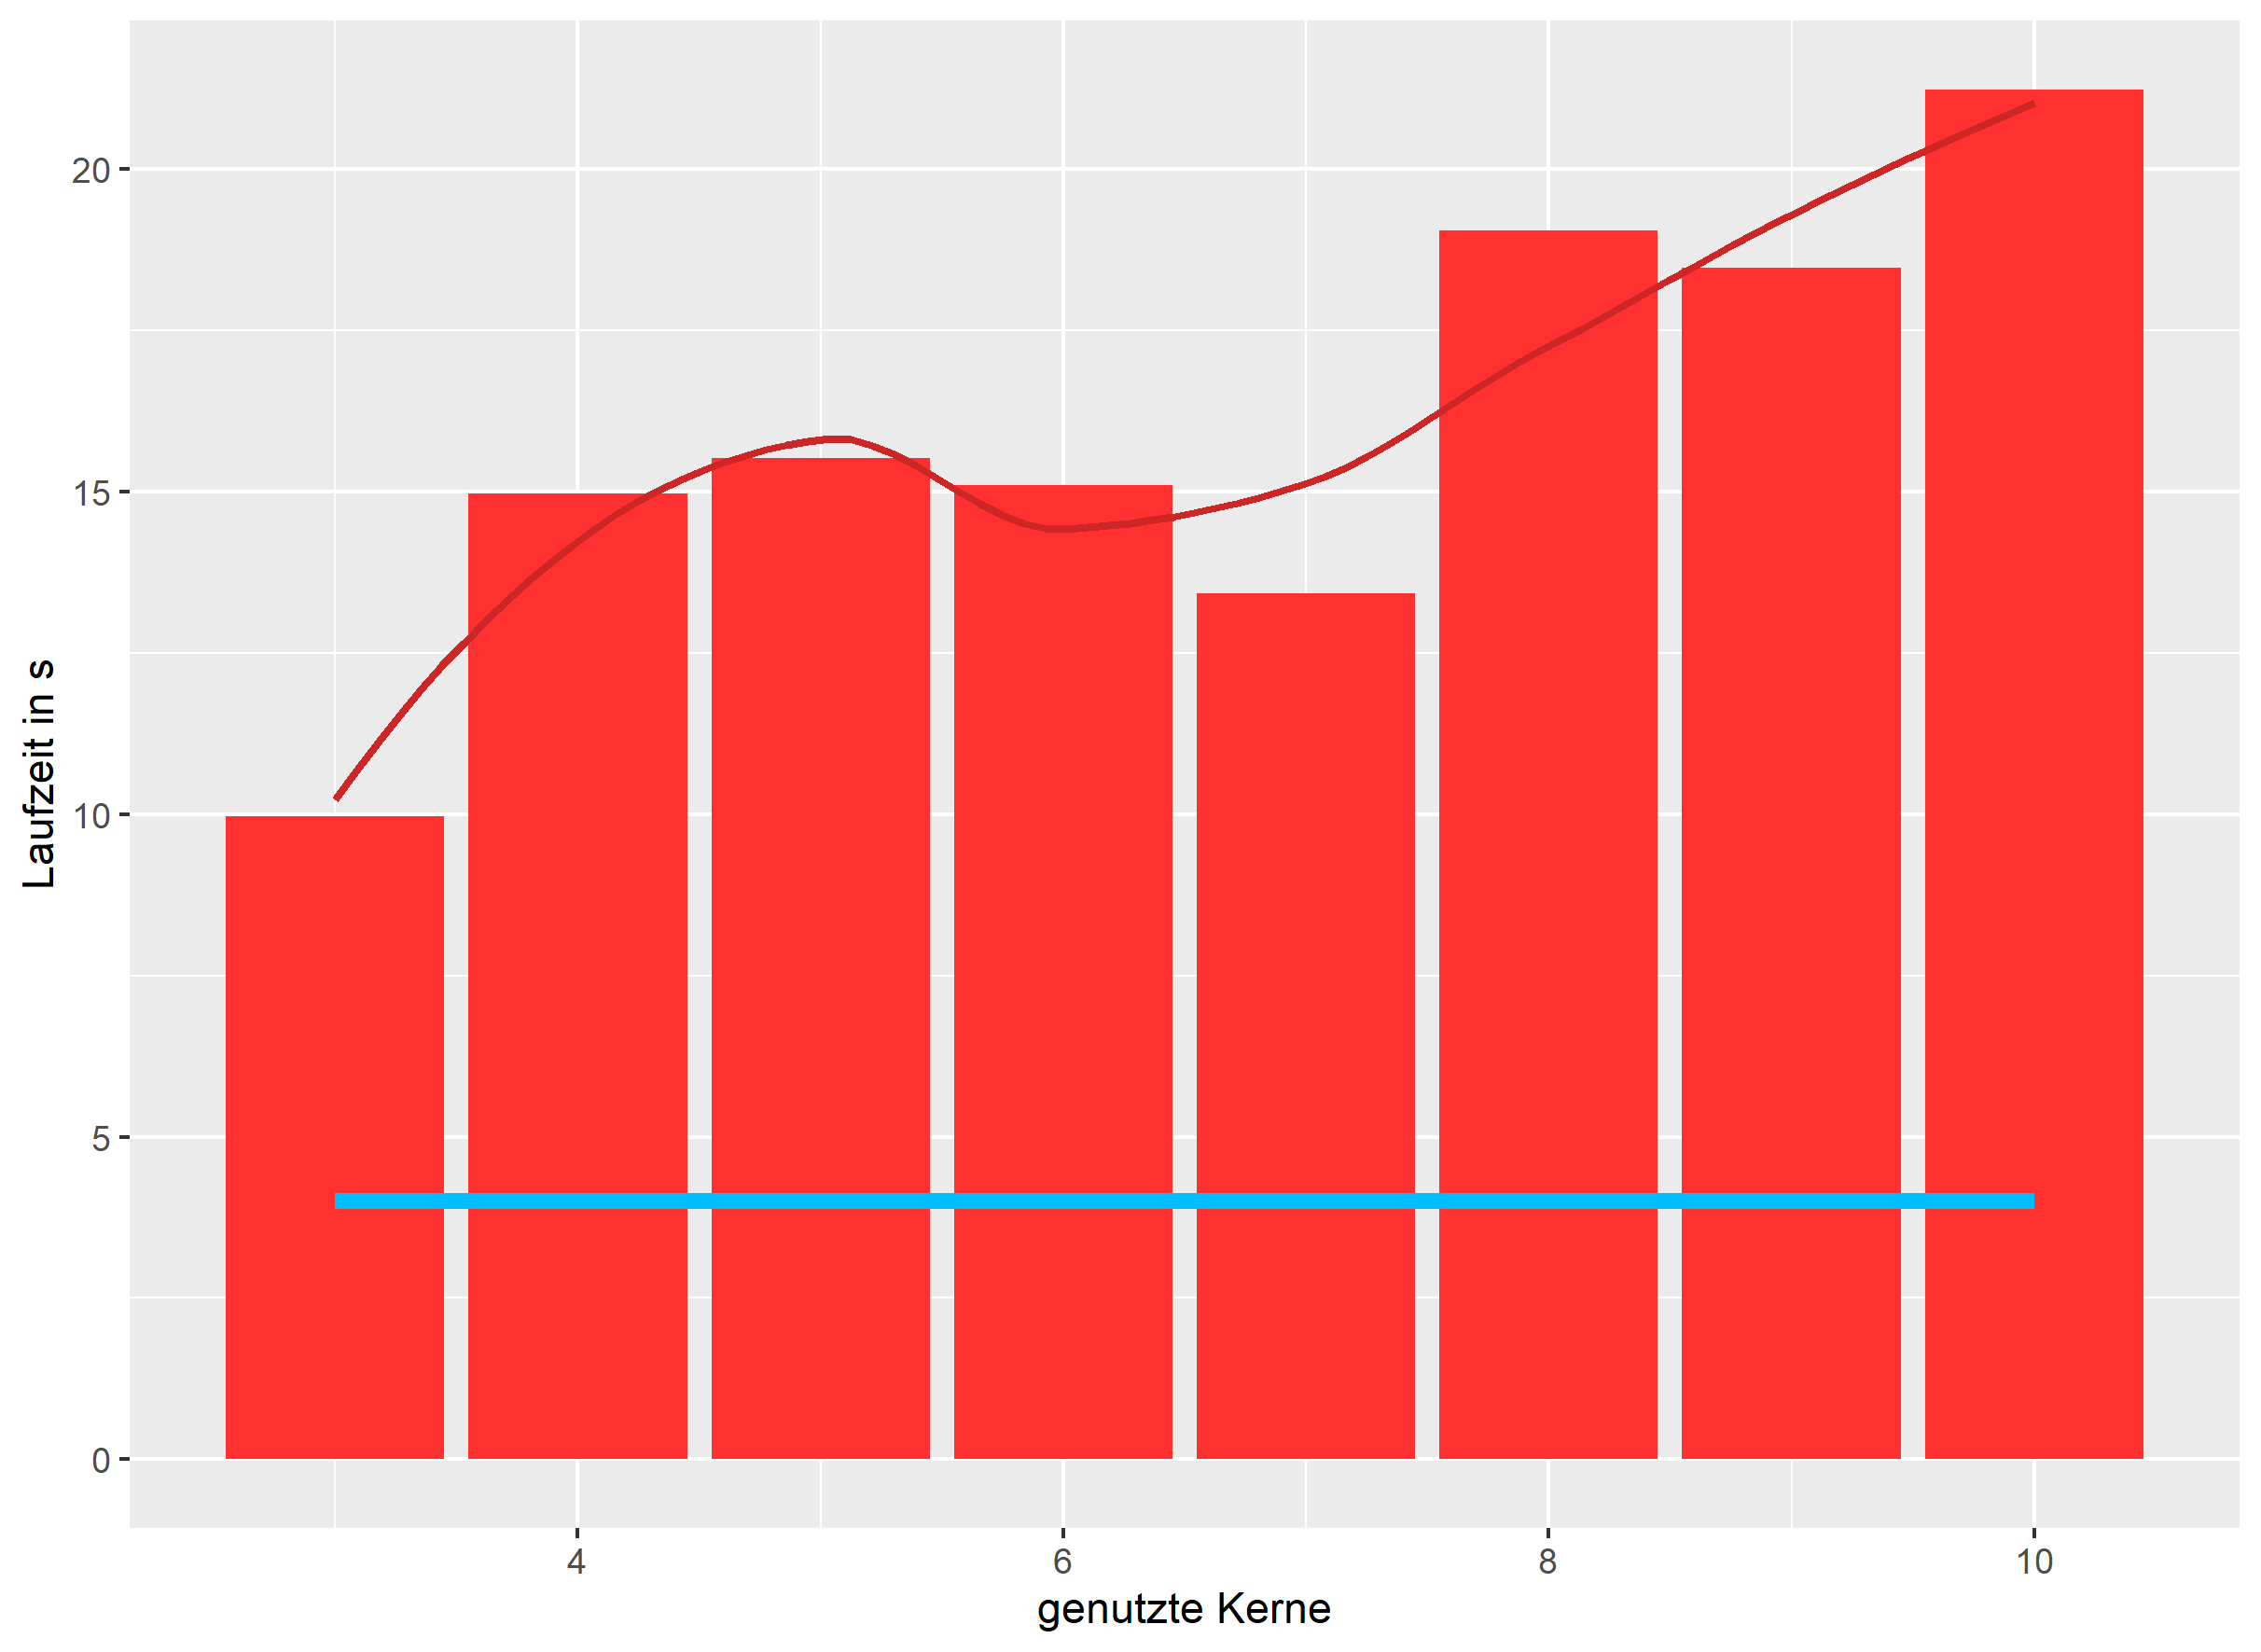
\includegraphics[width=0.55\textwidth]{Bilder/filter_kerne.png}
	\caption{Der Filter-Operator im Vergleich mit der Single-Thread-Variante (blaue Linie).}
	\label{img:filterKern}
\end{figure}

\subsection{Experimente}

\subsubsection{mThreadedSort}

Mit dem Multithread-Sortier-Operator habe ich zwei Experimente vorgenommen, nämlich einen Vergleich des Laufzeitverhaltens bei steigender Tupelzahl in den Relationen für einfache Suchattribute und Mehrfach-Suchattribute sowie eine Untersuchung des Laufzeitverhaltens bei unterschiedlichem zur Verfügung stehendem Speicher und damit bei verschiedener Nutzung von Auslagerungsdateien.

\autoref{img:sortHeadExp} und \autoref{img:sortHeadMfExp} zeigen das Laufzeitverhalten am Beispiel der Sortierung der \Fb{buildings}-Relation nach der ID und der Relation \Fb{roads\-str} nach sechs Attributen, die so gewählt worden sind, dass für die Bestimmung der Reihenfolge meistens alle Attribute betrachtet werden müssen. Beide Verläufe zeigen, dass sich die Performance der Multithread-Variante mit der Relationsgröße gegenüber der Singlethread-Variante verschlechtert, allerdings in einem deutlich anderem Ausmaß. Während bei der Sortierung nach einem Attribut die Laufzeit exponentiell wächst, liegt bei vielen Sortierattributen, also wesentlich mehr Vergleichen innerhalb des Operators, ein lineares Wachstum vor, wenn auch mit einer stärkeren Steigung beim von mir implementierten Operator. 

\begin{figure}
	\centering
	\subfloat[nach Größe der Relation\label{img:sortHeadExp}]{{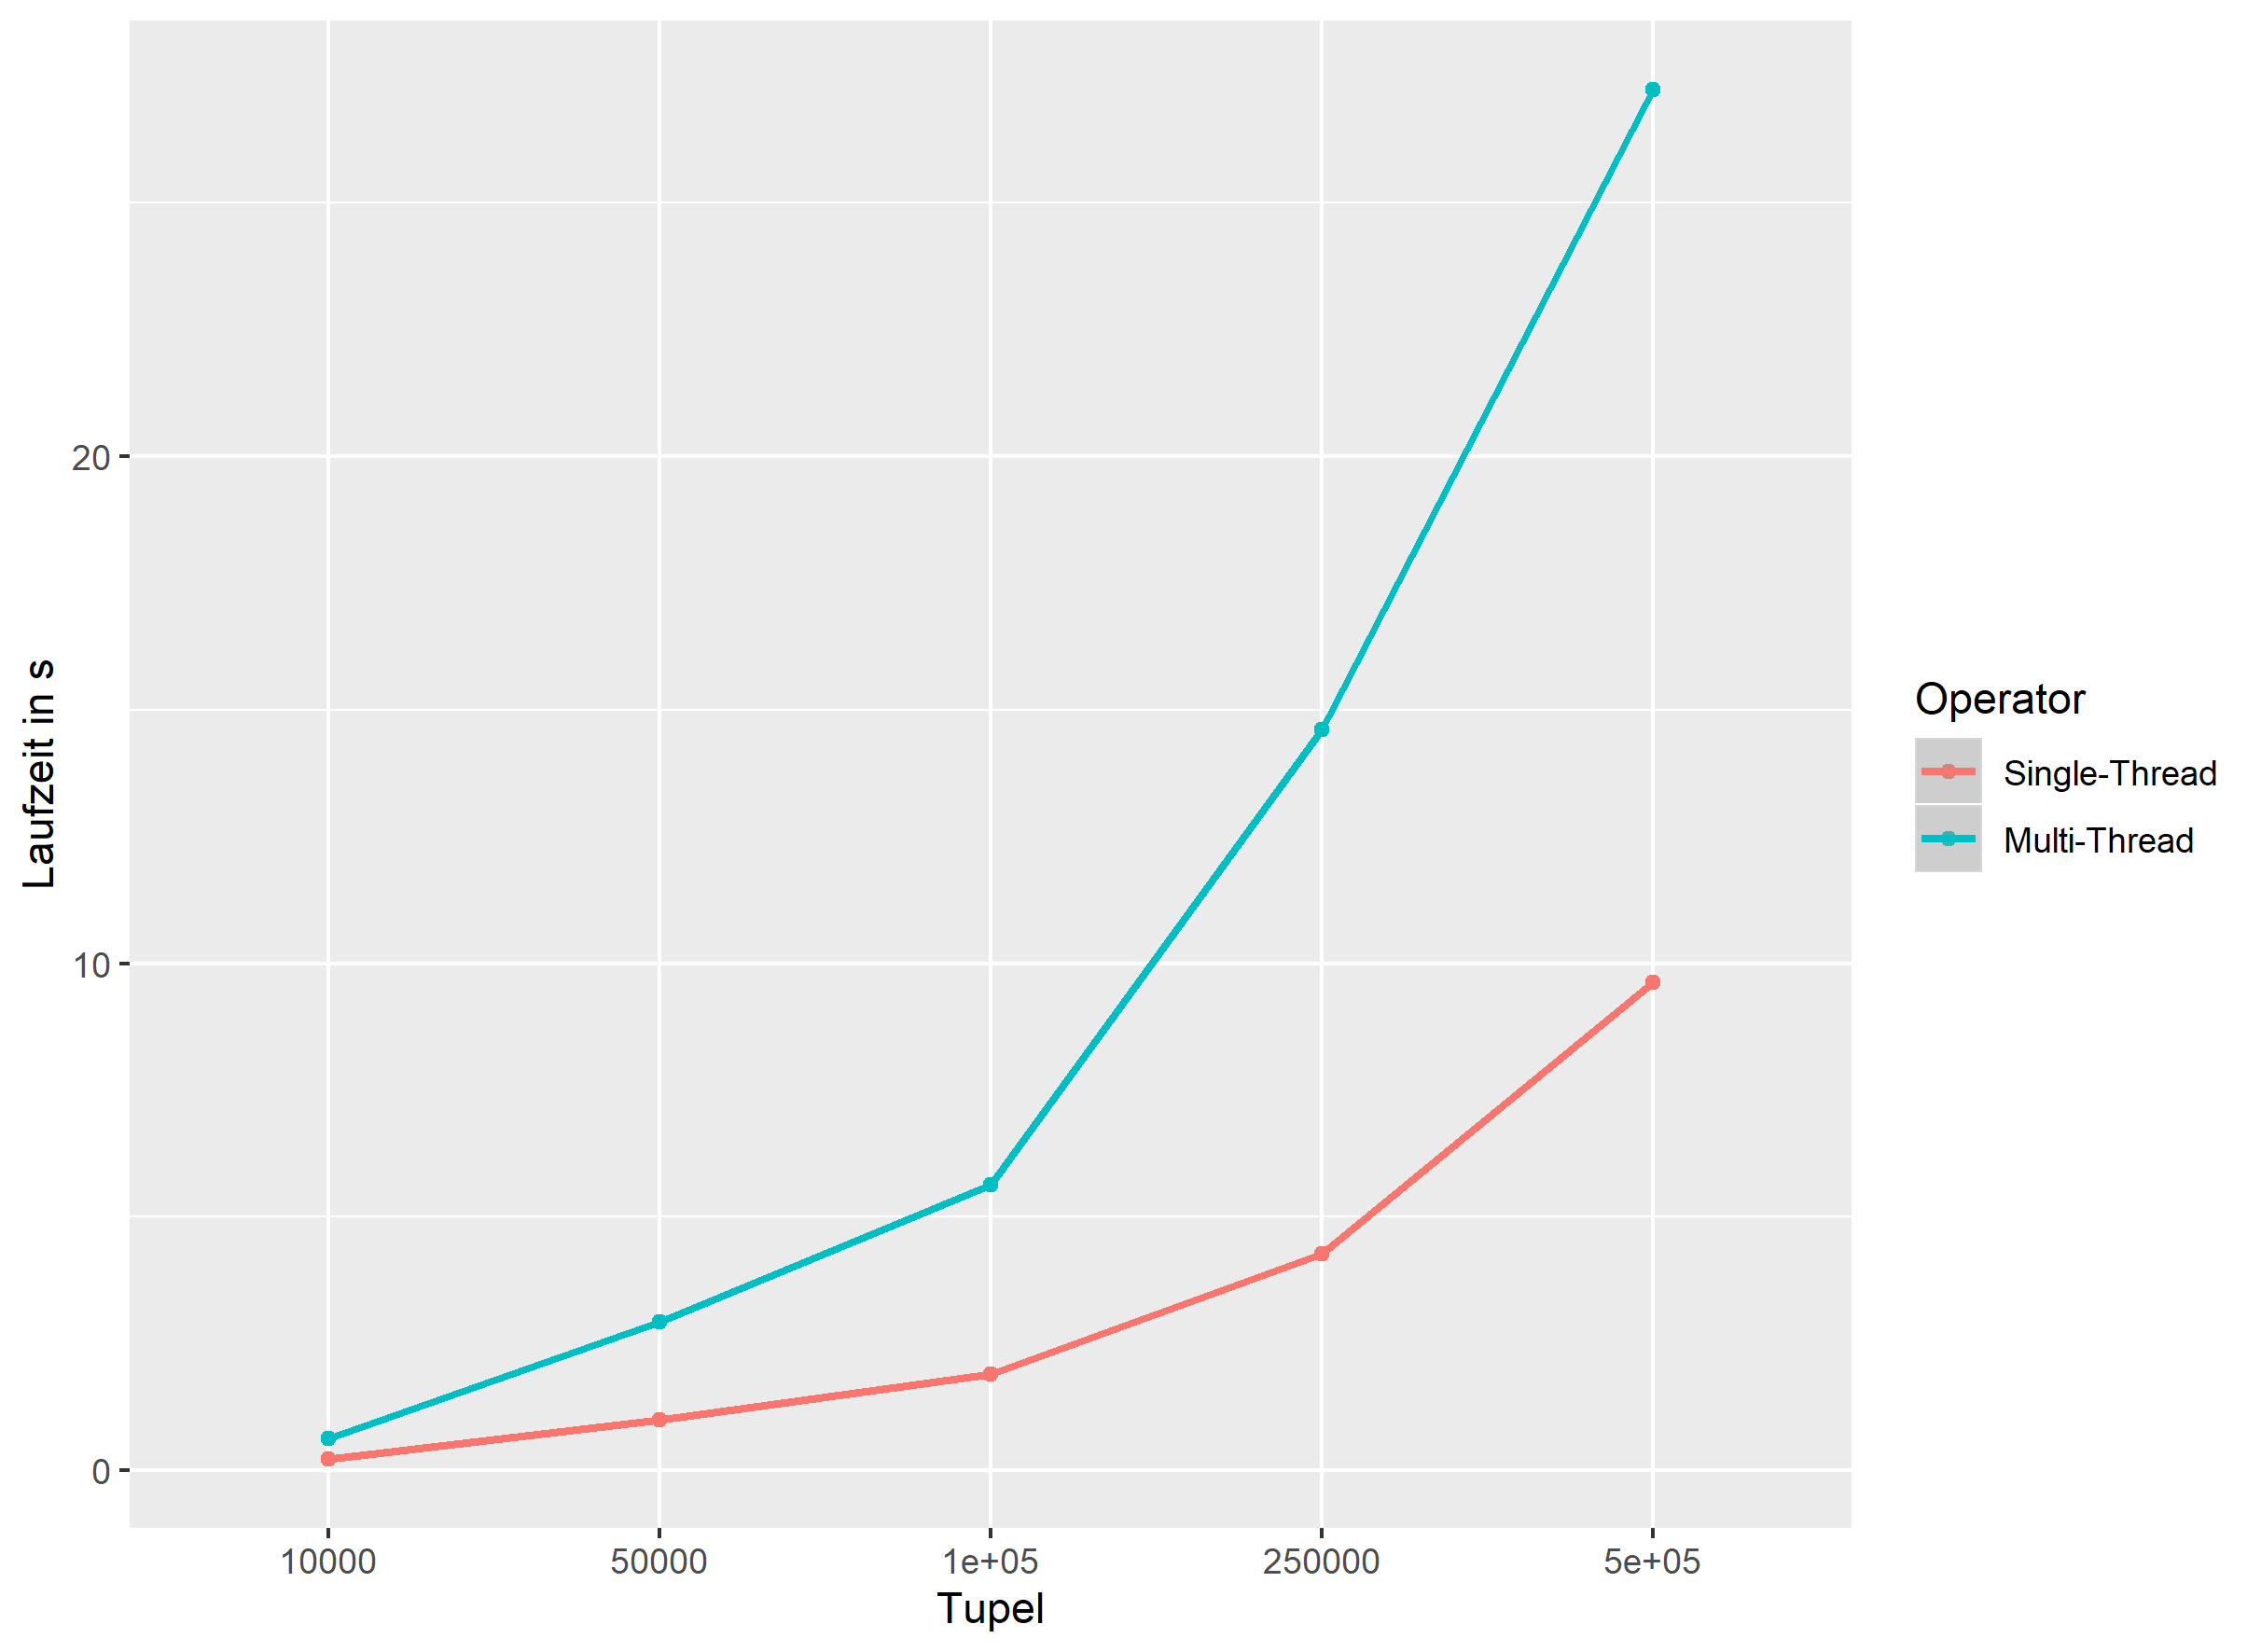
\includegraphics[width=0.45\textwidth]{Bilder/sort_head.png}}}
	\qquad
	\subfloat[zusätzlich mehrere Suchattribute\label{img:sortHeadMfExp}]{{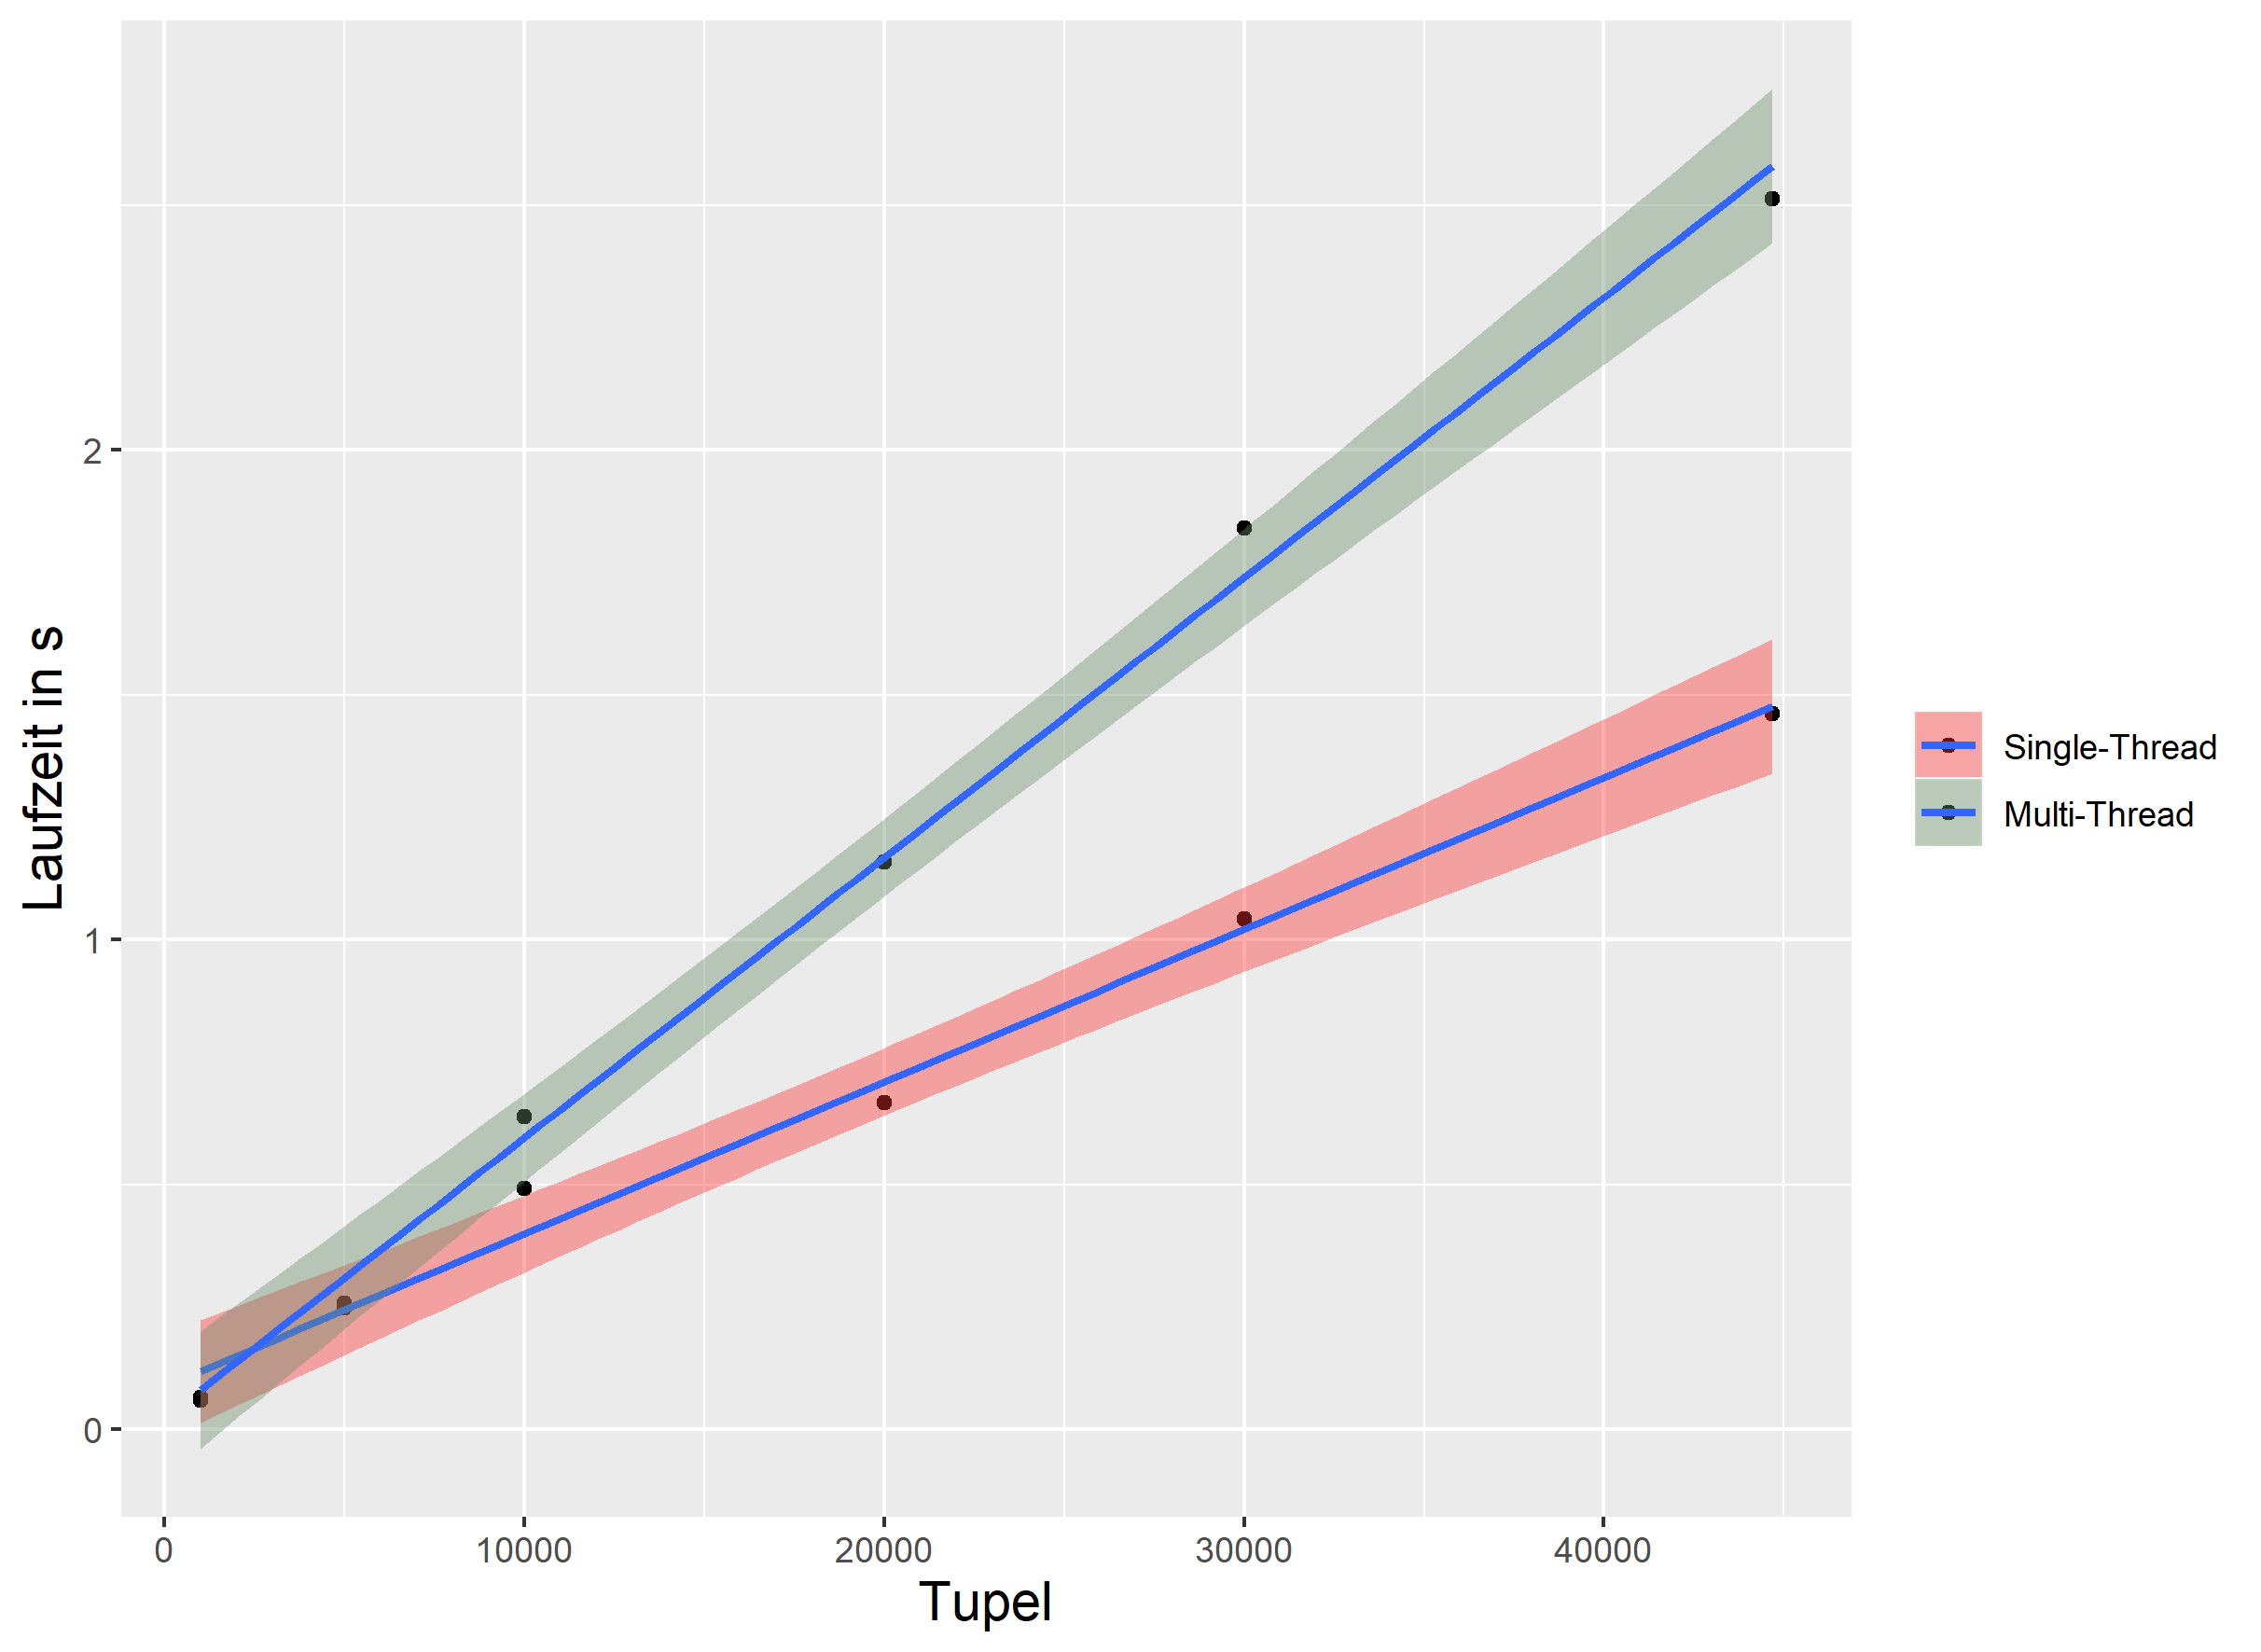
\includegraphics[width=0.45\textwidth]{Bilder/sort_head_mf.png}}}
	\qquad
	\subfloat[nach verfügbarem Speicher\label{img:sortMemExp}]{{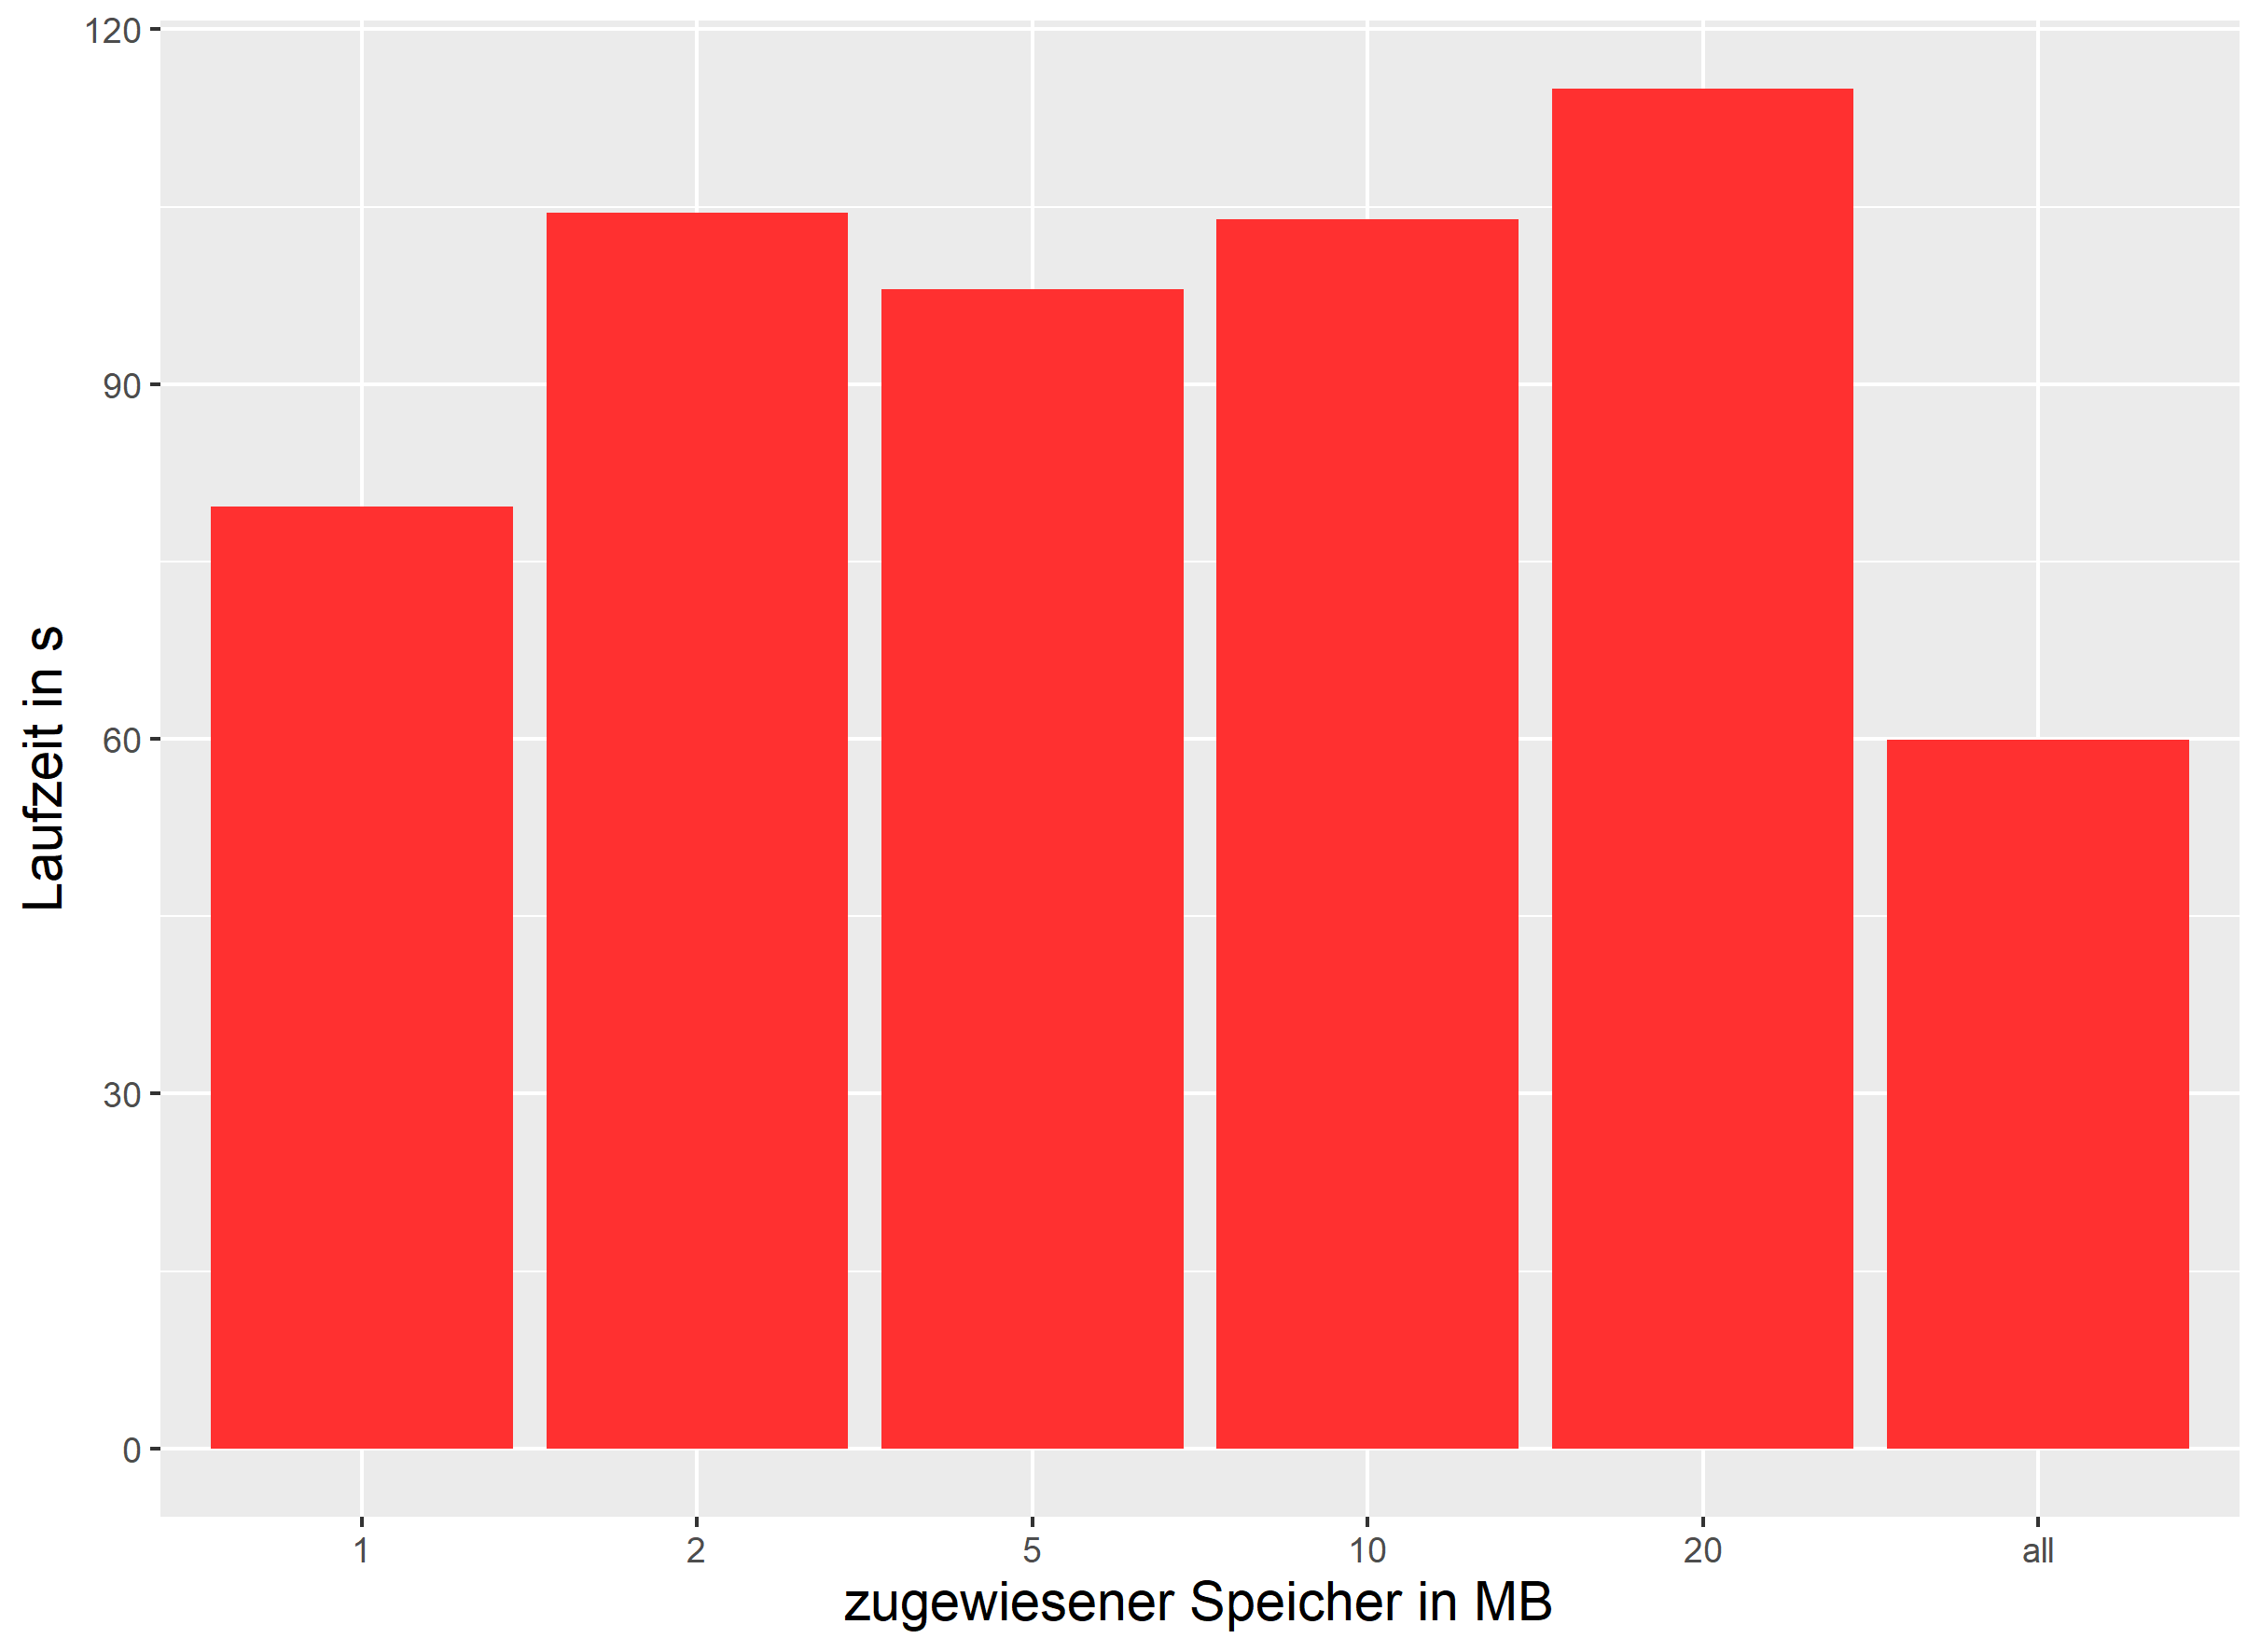
\includegraphics[width=0.35\textwidth]{Bilder/sort_mem.png}}}
	\caption{Experimente mit dem Sort-Operator.}
	\label{img:sortExpAllg}
\end{figure}

Der zur Verfügung stehende Speicherplatz für den Operator ist nur für die suboptimale Phase von Bedeutung und bestimmt, wie viele Läufe innerhalb dieser Phase generiert und verschmolzen werden müssen. \autoref{img:sortMemExp} zeigt die Laufzeit der Sortierung der Relation \Fb{buildings} nach der ID bei unterschiedlichem zur Verfügung stehendem Hauptspeicher. Deutlich ist der Sprung von 20 auf 40~MB. Hier nehme ich an, dass bei 40~MB keine Auslagerungsdateien mehr notwendig sind. Warum die Laufzeit bis 20~MB mit kleinen Abweichungen ansteigt, liegt wahrscheinlich an einer ungünstigen Verteilung auf die Läufe oder aber an den Schwankungen, die bei der Laufzeitmessung möglich sind (vgl. \autoref{te}).


\subsubsection{mThreadedHybridJoin}
\label{exp:hash}

Für den Hashjoin-Operator untersuche ich sein Verhalten gegenüber Änderungen des Speicherplatzes, der ihm zur Verfügung steht, gegenüber der wachsender Tupelzahl in der R- und S-Relation sowie wie sich die Konfigurierung der Hashtabellen auf sein Laufzeitverhalten auswirkt \autoref{img:joinBucket}.

Eine Analyse, inwieweit sich die Performance des Operators verändert, wenn ihm unterschiedlich viel Speicherplatz zur Verfügung steht, wurde mit einem Selfjoin der Relation \Fb{roads\_str} vorgenommen \autoref{img:joinMemExp}. Wenn weniger Speicher zur Verfügung steht, bedeutet dies vor allem, dass Teile der Hashtabellen ausgelagert werden und eventuell ein rekursiver Aufruf des Verschmelzungs-Algorithmus notwendig wird. Dies ist allerdings vor allem dann der Fall, wenn die R-Relation bezüglich des Joinattributs sehr ungleich verteilt ist. Die Tendenz der Laufzeit bei steigendem zur Verfügung stehenden Speicher ist zwar deutlich abnehmend, aber die Abweichungen von der Regressionsgeraden sind sehr ausgeprägt. Deswegen gehe ich anders als erwartet davon aus, dass nicht mit Sicherheit festgestellt werden kann, dass eine Auslagerung von Buckets in Dateien eine große Auswirkung auf das Laufzeitverhalten hat.

\begin{figure}
	\centering
	\subfloat[Vergleich nach verfügbarem Speicherplatz\label{img:joinMemExp}]{{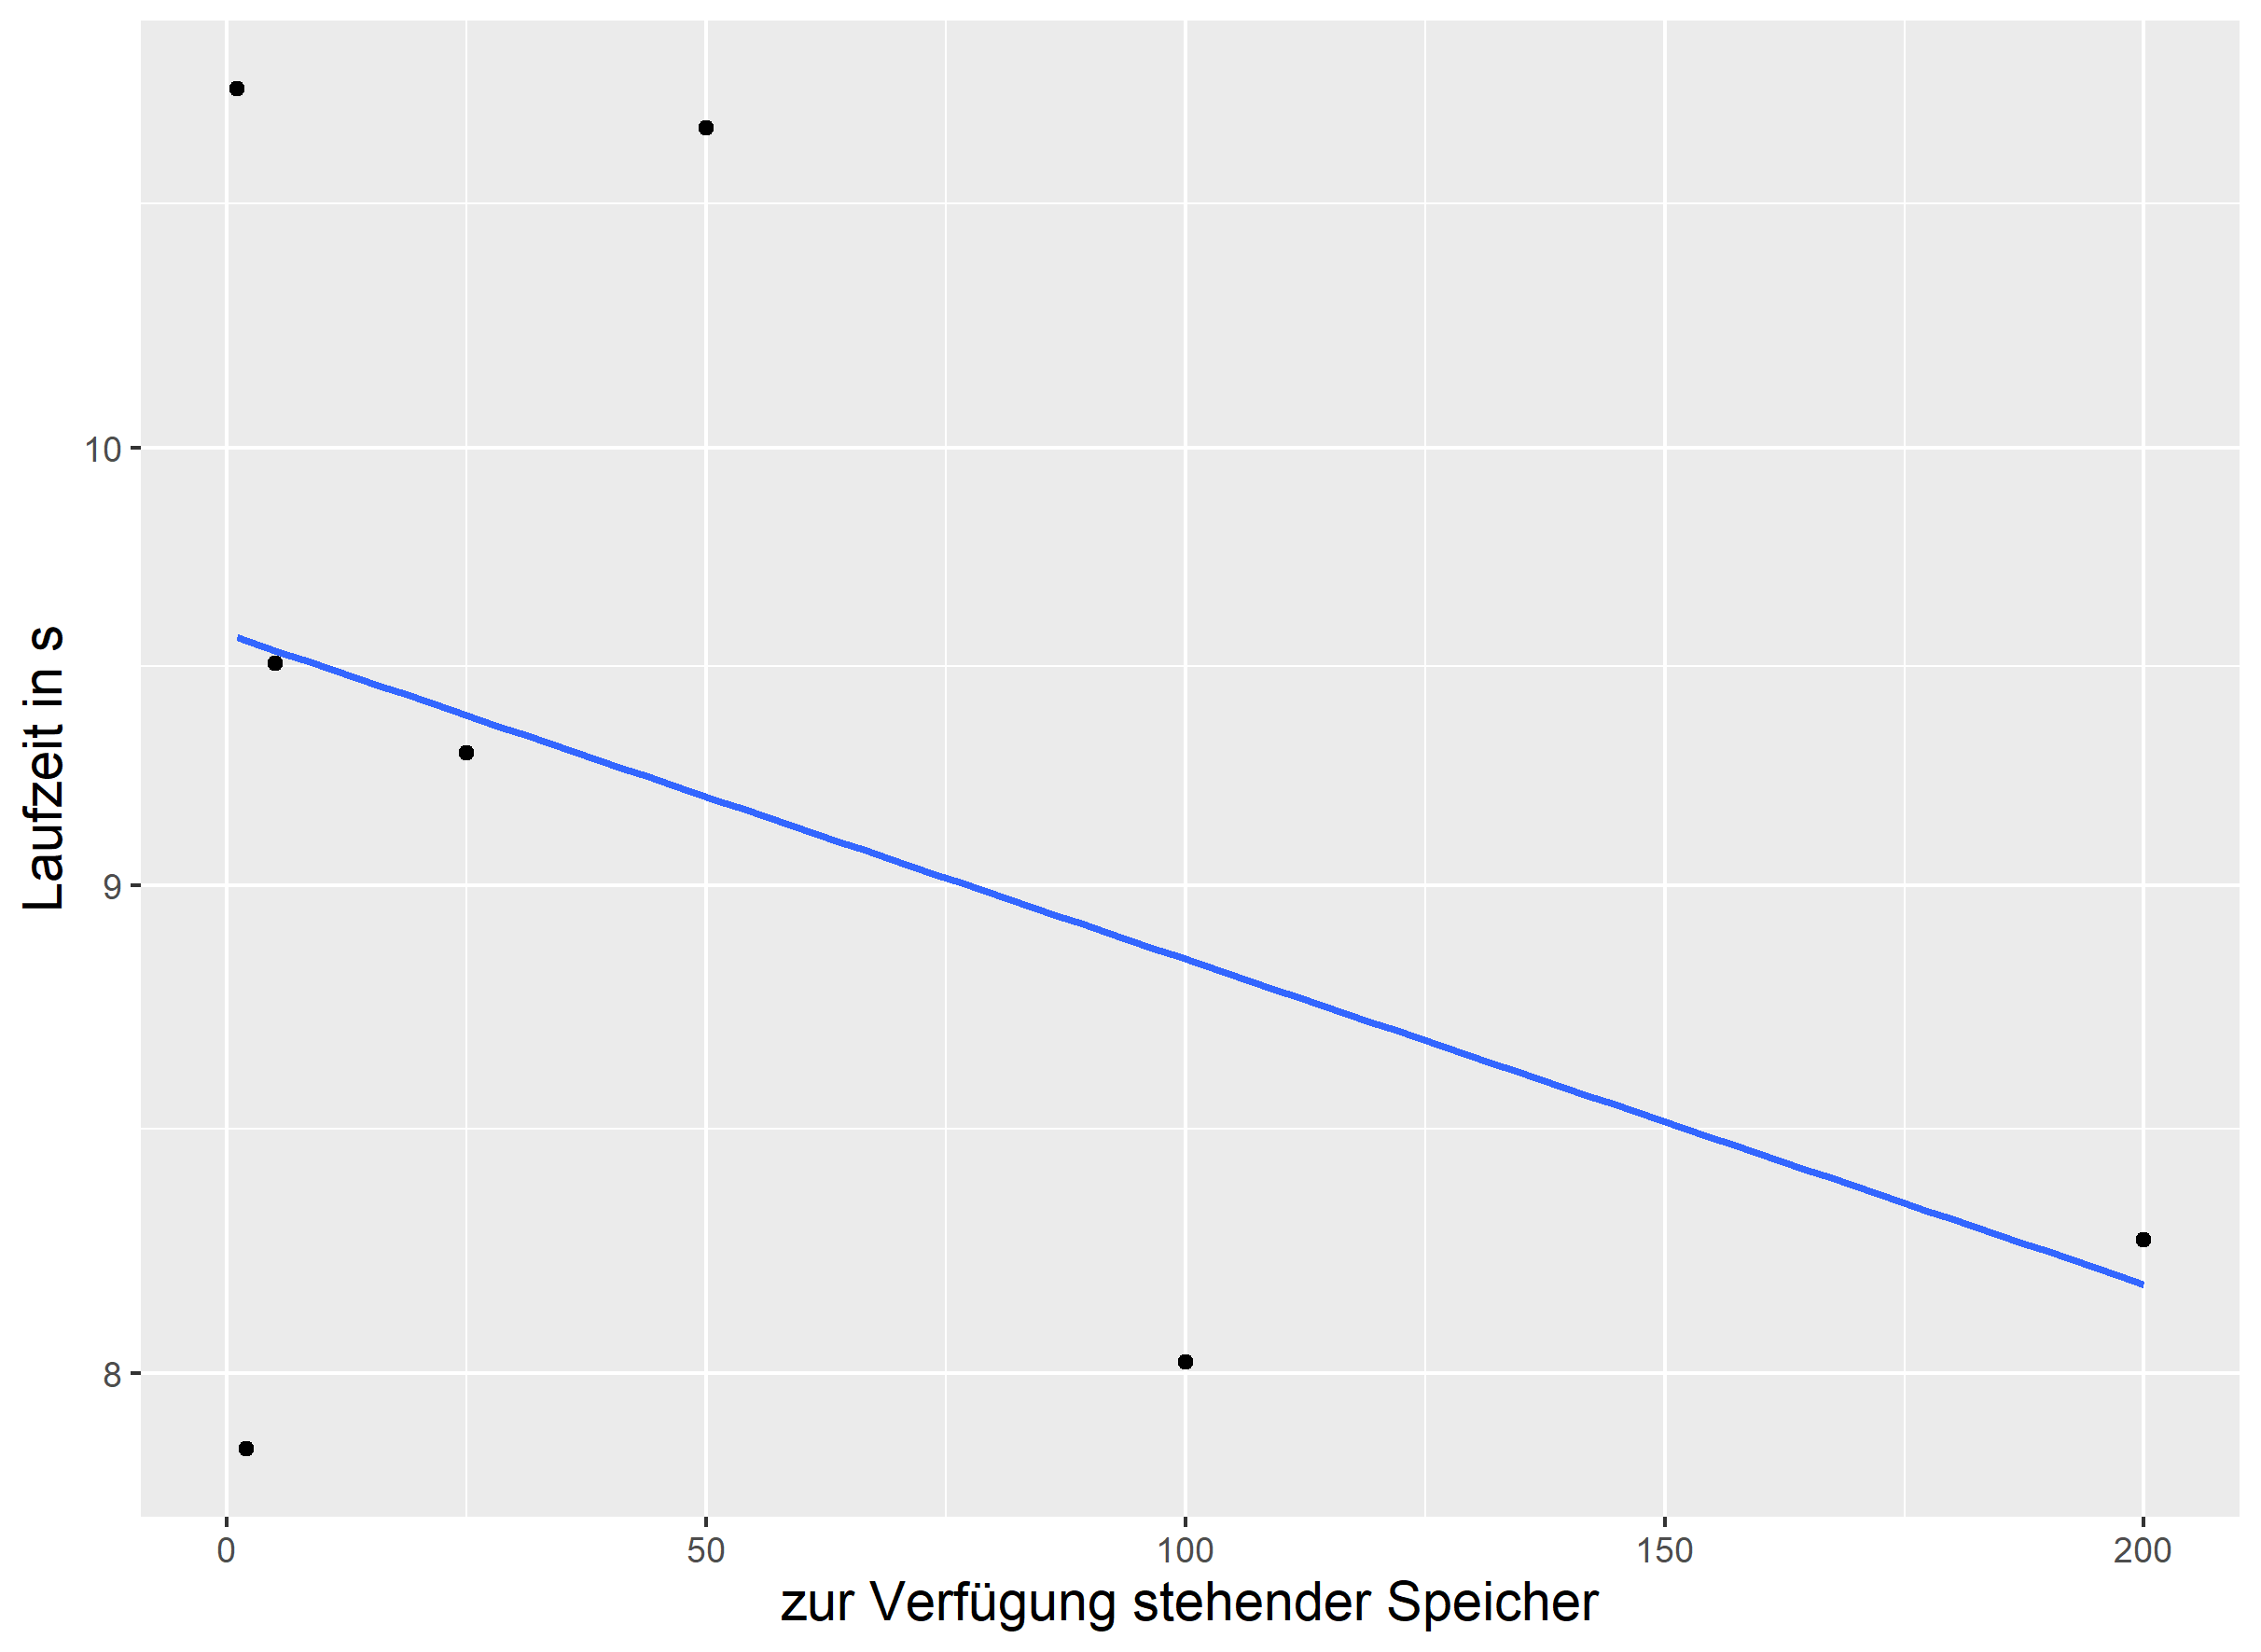
\includegraphics[width=0.45\textwidth]{Bilder/join_mem.png}}}
	\qquad	
	\subfloat[Vergleich nach Größe der Relation\label{img:joinHeadExp}]{{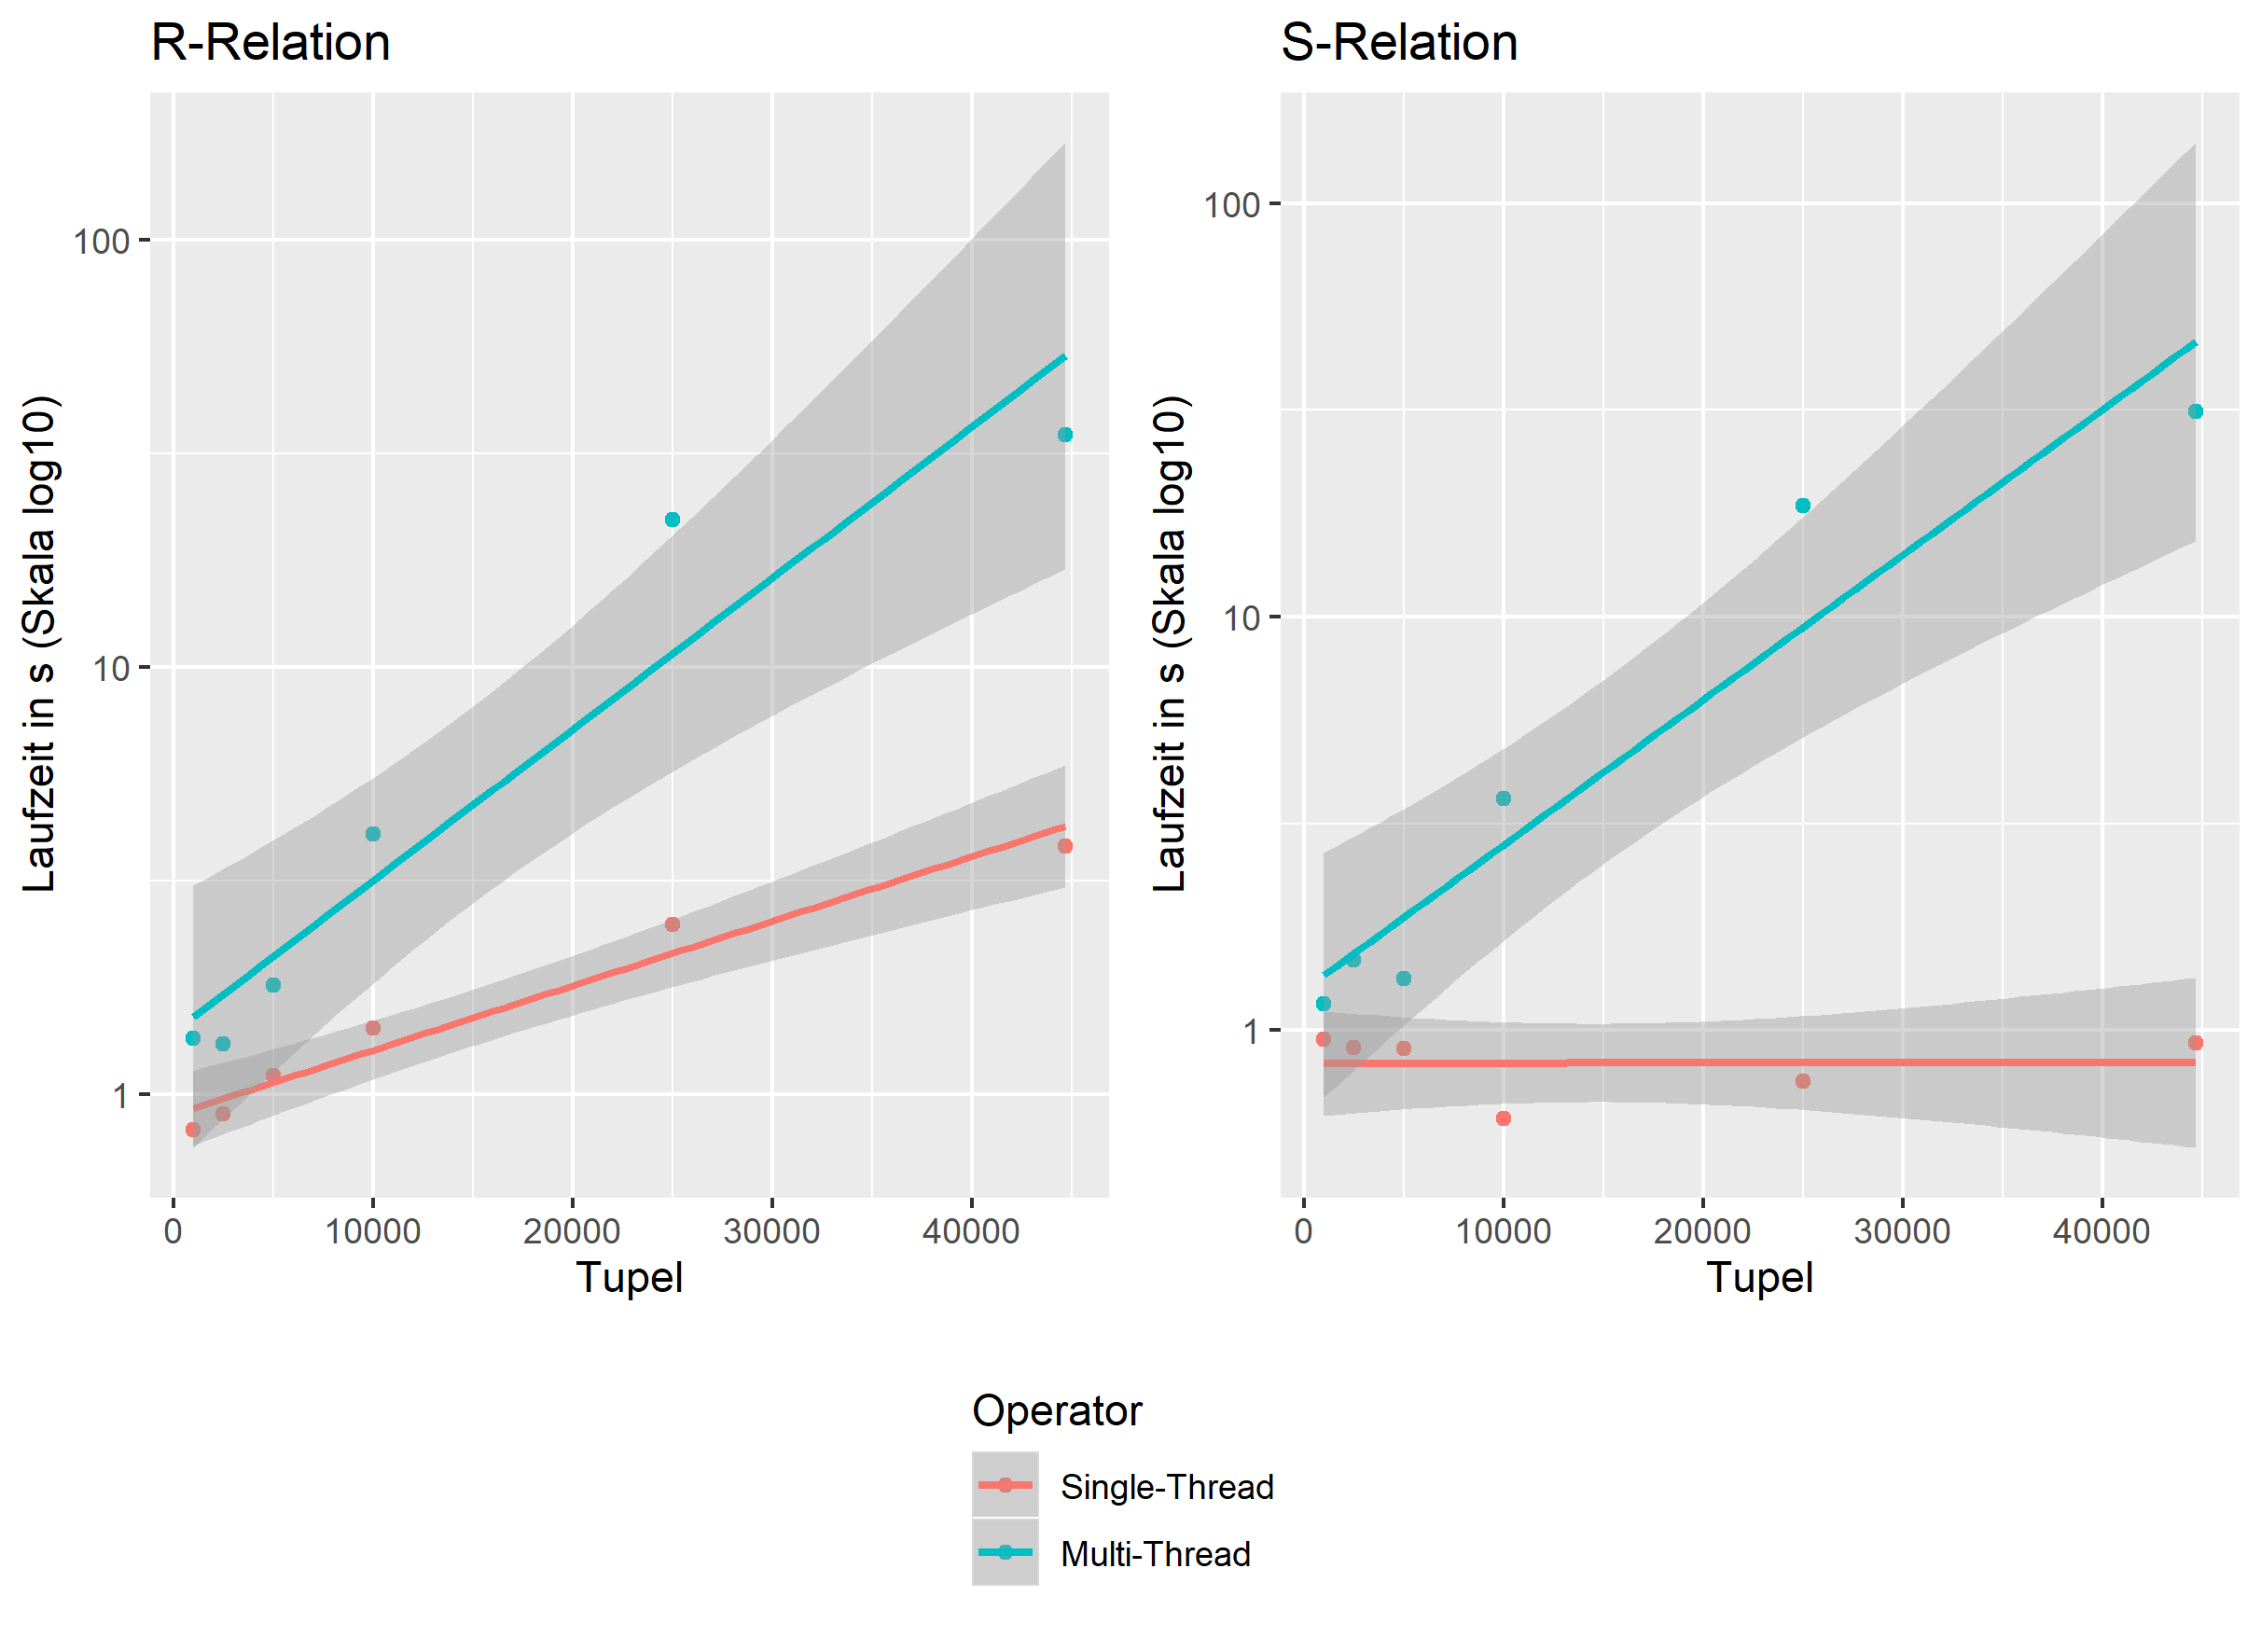
\includegraphics[width=0.45\textwidth]{Bilder/join_head_self2.png}}}
	\caption{Selfjoin \Fb{roads\_str}.}
	\label{img:joinExpAllg}
\end{figure}

Im Gegensatz zum Verhalten gegenüber dem Speicher, der dem Operator zugewiesen worden ist, zeigt das Verhalten gegenüber der Relationsgröße ein eindeutiges Bild \autoref{img:joinHeadExp}. Große Relationen erhöhen die Laufzeit des von mir implementierten Operators linear. Die lineare Regressionsgerade hat bei wachsender R-Relation für den Multithread-Operator eine stärkere Steigung als die Singlethread-Variante. Interessant ist es vor allem, dass bzgl. einer wachsenden S-Relation sich das Laufzeitverhalten des von mir implementierten Operators in ähnlicher Weise verschlechtert wie bei wachsender S-Relation, aber die Singlethread-Variante hier jenseits von kleinen Schwankungen keine Laufzeitveränderung aufzeigt. Dies deutet an, dass ich ungünstige Entscheidungen für die Implementierung des Hybrid-Hash-Algorithmus getroffen habe. Einige Ideen, wie die Implementierung des Multithreading-Hybrid-Hashs verbessert werden kann, habe ich bereits in \autoref{impl:hybrid} erläutert.   

\begin{figure}
	\centering
	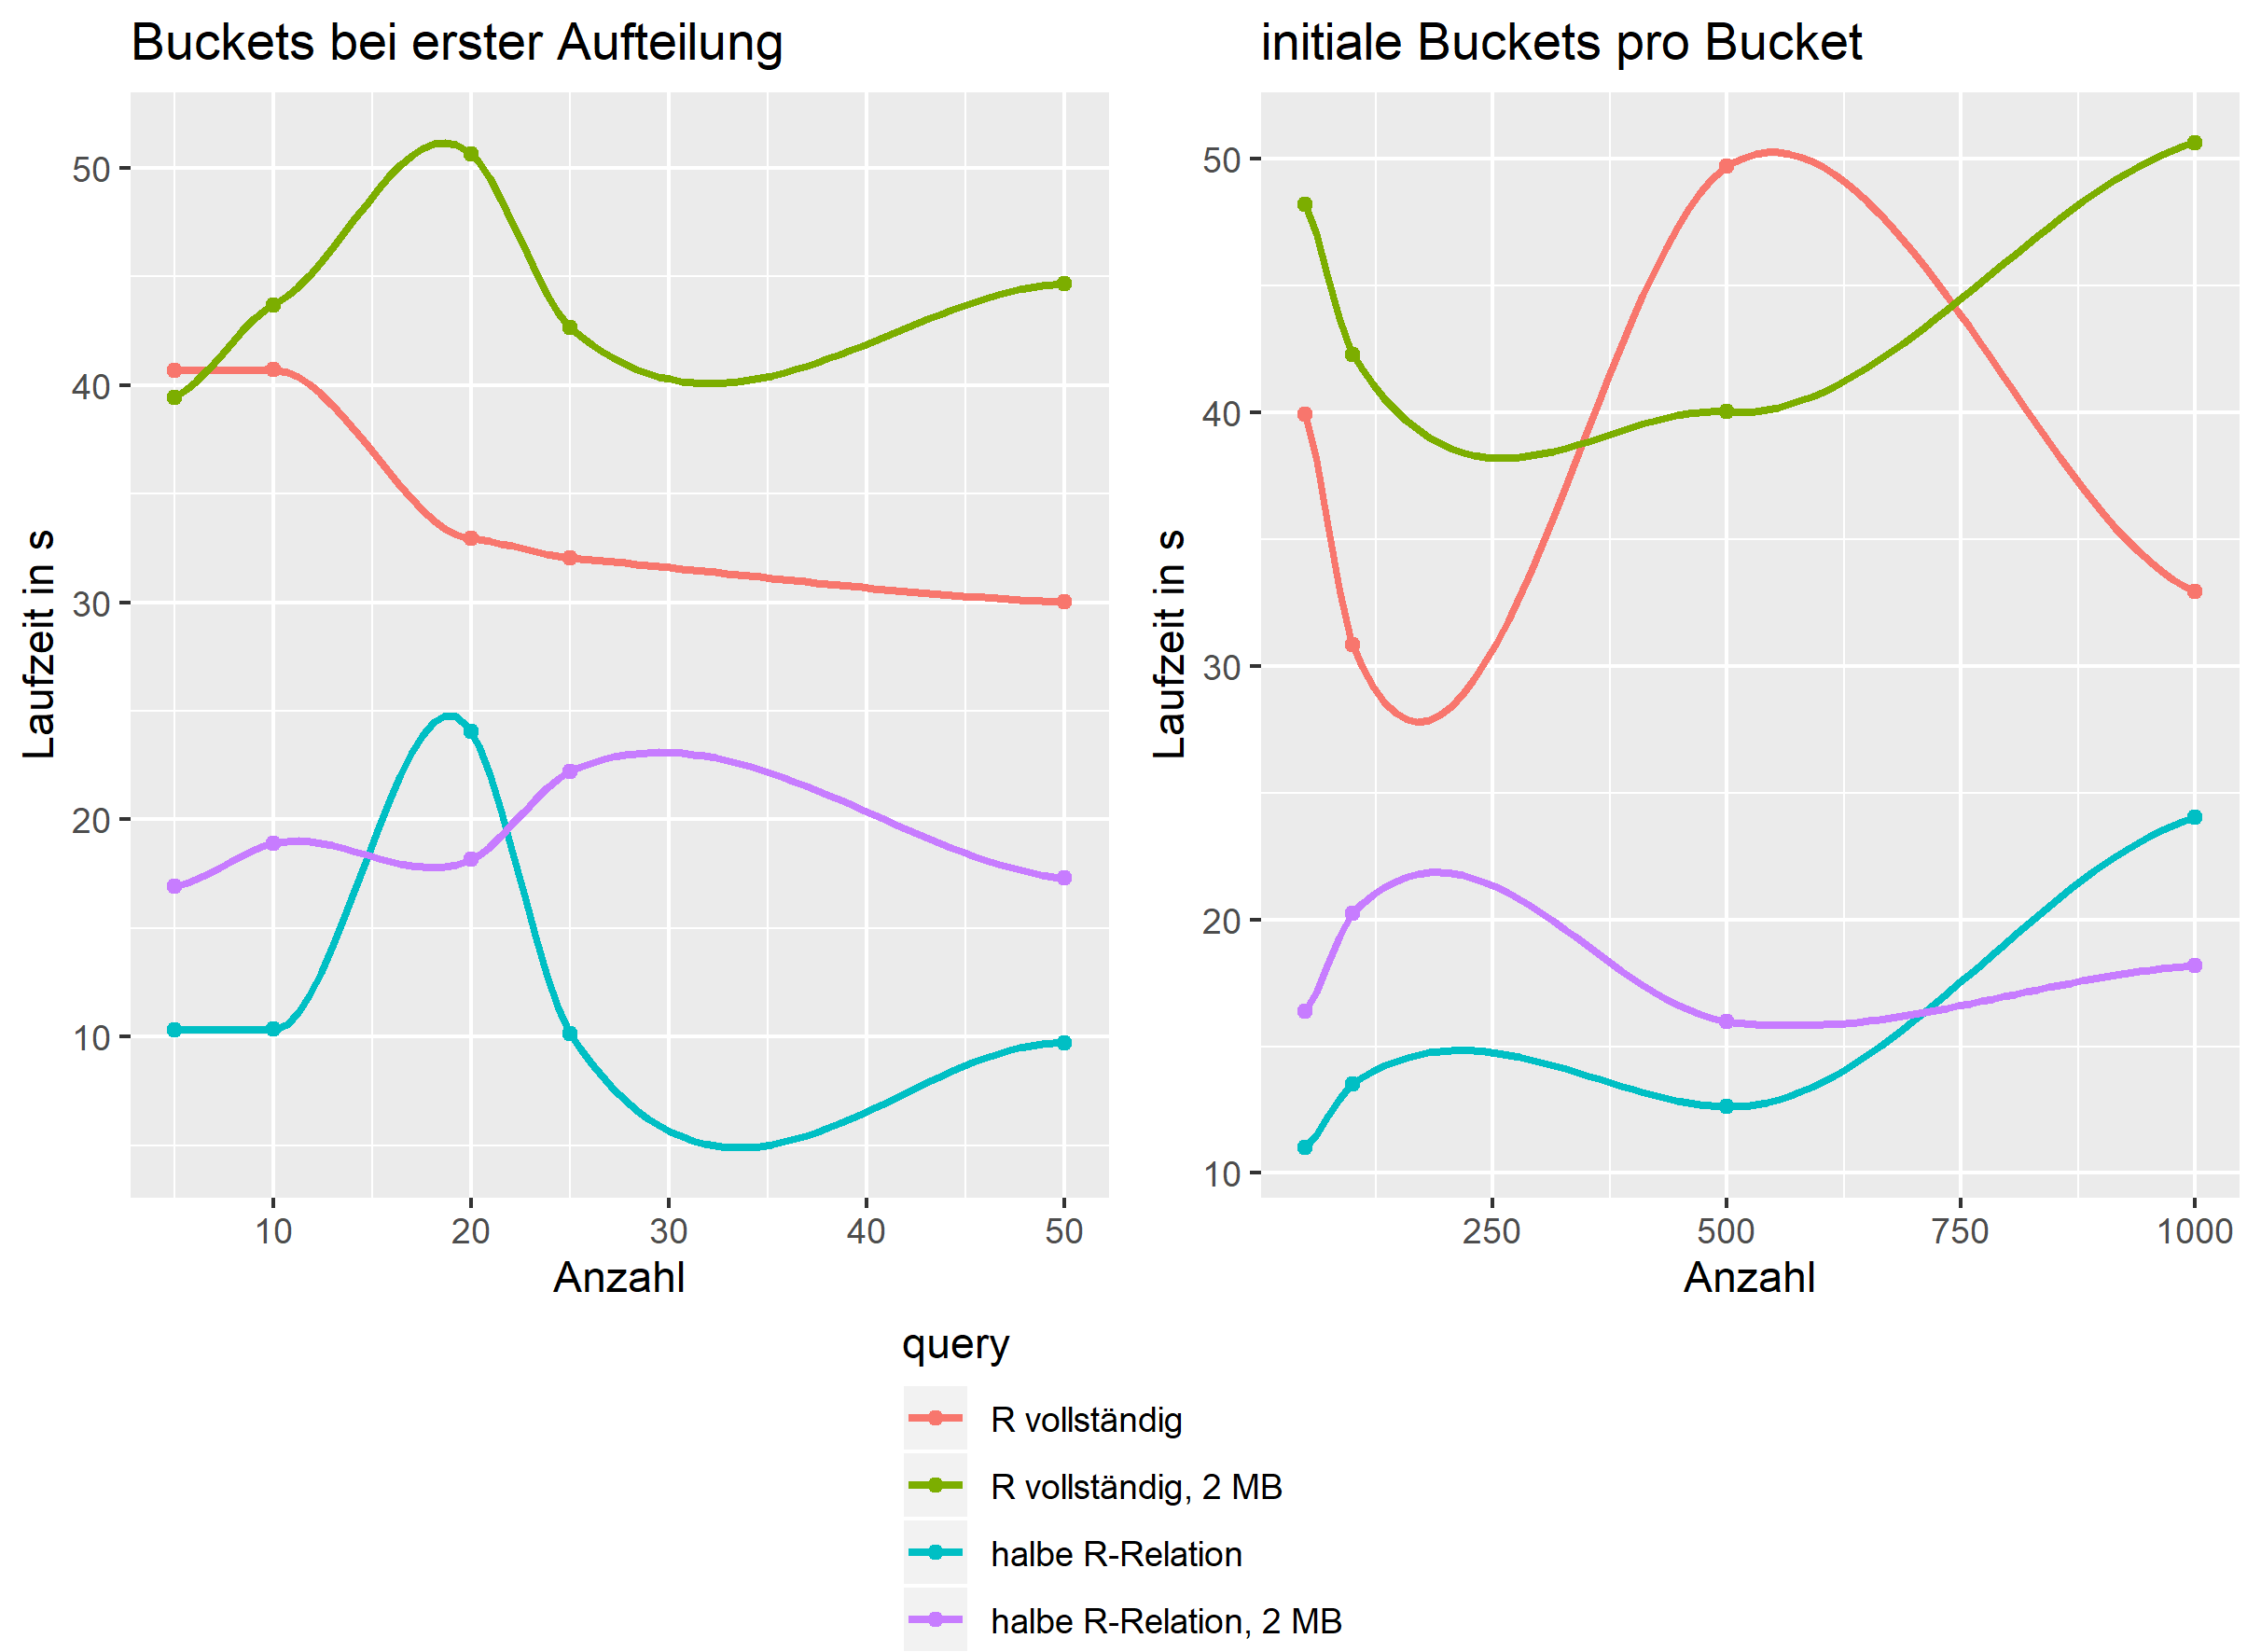
\includegraphics[width=0.70\textwidth]{Bilder/join_bucket.png}
	\caption{Selfjoin der Relation \Fb{roads\_str} nach dem Straßenname bei Veränderung der Anzahl von Buckets.}
	\label{img:joinBucket}
\end{figure}

Der von mir implementierte Hybrid-Hash-Join teilt den Tupelstrom drei Mal in Buckets auf: für die Partitionierung auf die Threads, dann innerhalb jedes Threads auf eine kleine Zahl Buckets, von denen der Erste direkt verarbeitet wird und abschließend jedes Bucket in jedem Thread in so viele Buckets, dass in jedem Bucket sich möglichst nur ein Tupel befindet. Für die letzte Aufteilung wird ein initialer Wert verwendet. \autoref{img:joinBucket} zeigt Glättungskurven für die Veränderung der Laufzeit einerseits nach der Bucketzahl der ersten Aufteilung im Thread und andererseits nach der initialen Bucketzahl, die in jedem Bucket im Thread wiederum angelegt werden (für die erste Aufteilung im Thread wird hier der Standardwert 20 verwendet). Jenseits der Bucketzahl wurde auch die Größe der R-Relation verändert und der zur Verfügung stehende Speicher reduziert, damit Auslagerungen und rekursive Aufteilungen von nicht in den Hauptspeicher passenden Buckets vorgenommen werden müssen.

Die erste Aufteilung entscheidet vor allem darüber, inwieweit Buckets ausgelagert werden müssen. Optimal ist ein Wert, bei dem jeder Bucket in den Hauptspeicher passt und gleichzeitig die Anzahl der Buckets möglichst gering ist, da dann der erste Bucket, der direkt verschnitten wird, möglichst viele Tupel fasst. Negative Auswirkung hat es auch, wenn die Größe so gewählt wird, dass rekursive Ausführungen des Hash-Algorithmus notwendig werden, was vor allem dann auftritt, wenn die Relation bezüglich des Join-Attributs ungleich verteilt ist. Bei einer großen Relation und ohne eine Einschränkung des zur Verfügung stehenden Arbeitsspeichers gibt es dementsprechend einen Schwellwert für die Bucketzahl, an dem die optimale Speichernutzung erreicht ist und dementsprechend sich das Laufzeitverhalten deutlich ändert. Alle anderen Änderungen haben keine große Auswirkung. In allen betrachteten Beispielen gibt es nur eine kleinen Wertebereich für die Anzahl von Buckets, der sich negativ auf die Laufzeit auswirkt.

Die Anzahl initialer Sub-Buckets gilt nur für das erste der 20 Buckets in jedem Thread, der direkt verschnitten wird, da er anschließend aus der durchschnittlichen Größe jedes Buckets neu berechnet wird. Trotzdem hat seine Größe eine deutliche Auswirkung auf das Laufzeitverhalten. Sofern viele Tupel in das gleiche Bucket einsortiert werden, ist ein Verschmelzen über eine Schleife notwendig -- der Algorithmus nähert sich also einem Loop-Join an. Dementsprechend ist die Auswirkung stärker bei großen Relationen, da mehr Tupel auf eine Hashtabelle verteilt werden. Nach erreichen eines Optimums, bei dem jeder vorkommende Hashwert auf ein eigenes Bucket aufgeteilt wird, ist keine Veränderung mehr zu erwarten. Bis zu diesem Punkt verändert sich das Laufzeitverhalten schwankend, da es vorkommen kann, dass auch bei mehr verwendeten Buckets eine Verteilung ungleichmäßiger wird. Im Gegensatz dazu hat der zur Verfügung stehende Arbeitsspeicher für den Operator nur insofern einen Einfluss, dass weniger Tupel auf die Buckets verteilt werden müssen, sich also das Optimum früher einstellt und gleichzeitig die Schwankungen nicht so stark ausgeprägt sind, da im Durchschnitt auch weniger Tupel mit gleichen Hashwerten vorhanden sind.

\subsubsection{mThreadedSpatialJoin}
\label{exp:sj}

Um das Laufzeitverhalten des Multithreading-Spatial-Joins zu verstehen, habe ich folgende unterschiedliche Experimente durchgeführt: Bei verschiedenen Relationen, einem Selfjoin von \Fb{roads} und $waterways \bowtie roads$, habe ich die Größe der R- und S-Relation variiert (\autoref{img:sjExpHeadAllg}). Bei einer Verschmelzung der Relationen \Fb{roads} und \Fb{landuse} habe ich dem Operator unterschiedlich viel Arbeitsspeicher zur Verfügung gestellt \autoref{img:sjMemExp} und bei dem gleichen Join die Konfiguration des verwendeten R-Baums bei unterschiedlich großen Relationen variiert \autoref{img:sjTreeExp}. Abschließend betrachte ich einen Vergleich des Laufzeitverhaltens mit und ohne einer Kompilierung von \Fb{Secondo} mit dem Flag, welches die Threadsicherheit steuert {\autoref{img:sjSync}}. 

\begin{figure}[H]
	\centering
	\subfloat[Selfjoin\label{img:sjHeadExpRr}]{{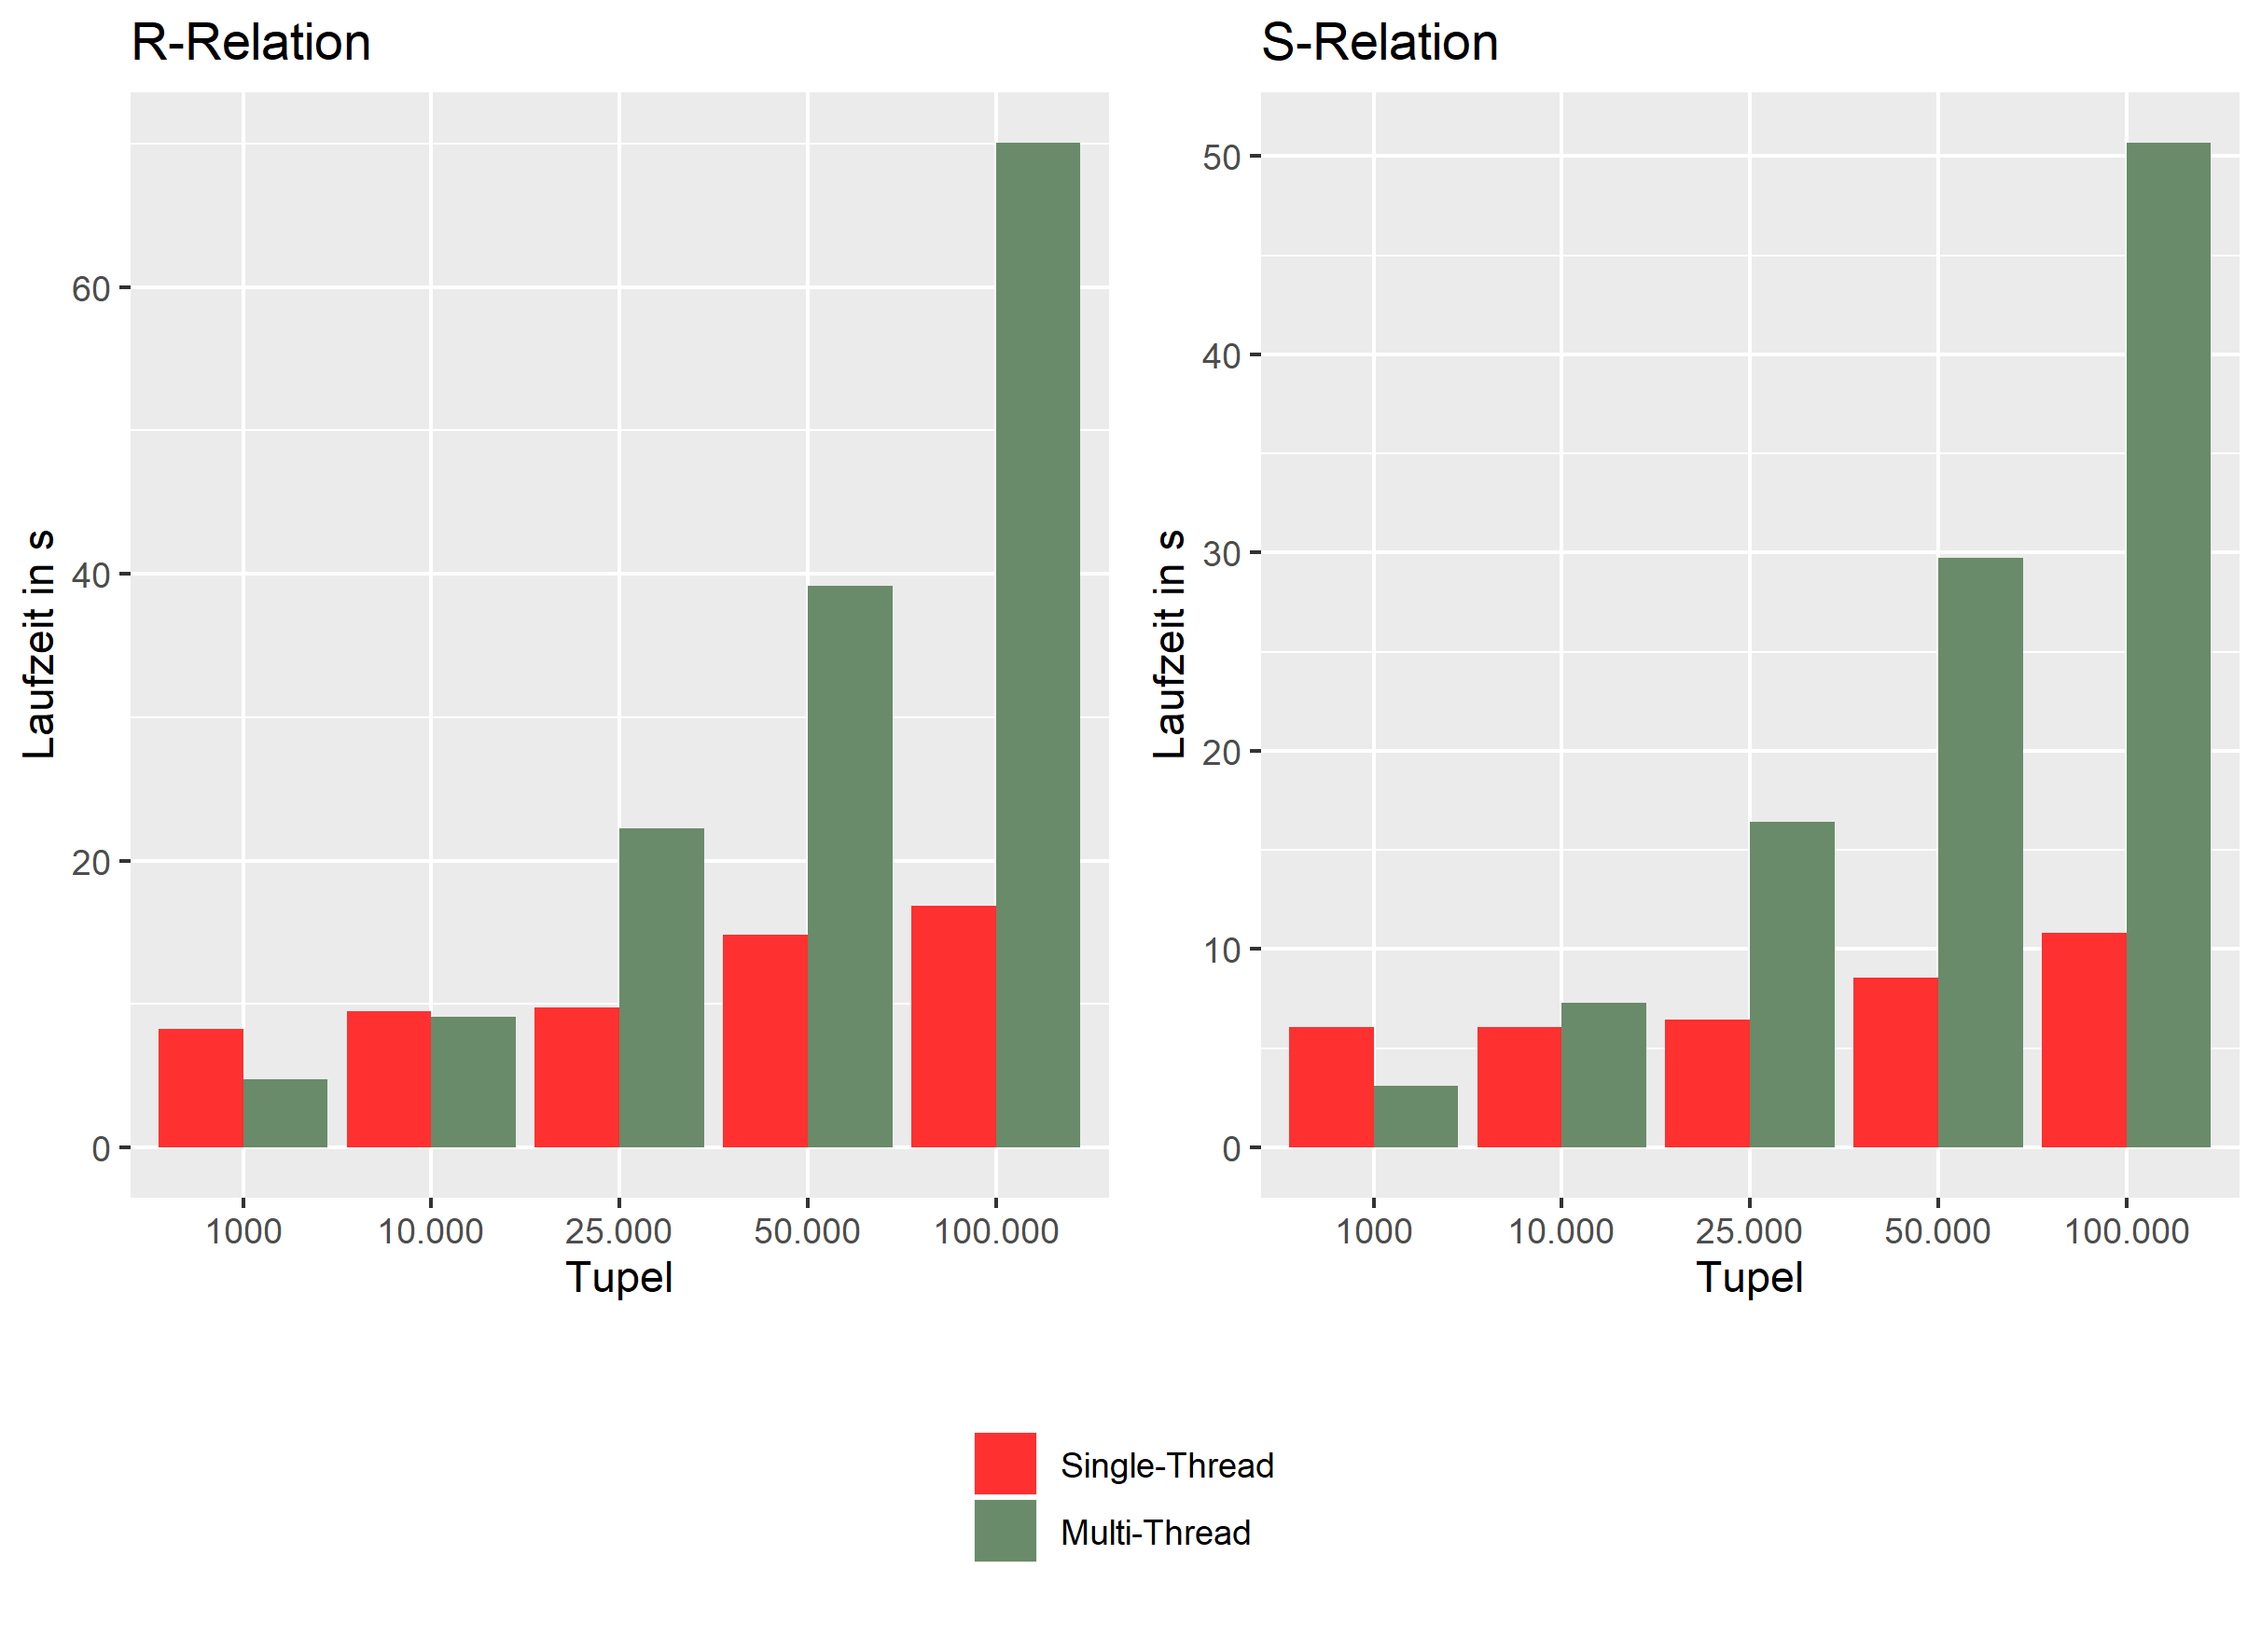
\includegraphics[width=0.6\textwidth]{Bilder/sj_head_rr.png}}}
	\qquad	
	\subfloat[$waterways \bowtie roads$ bzw. $roads \bowtie waterways$\label{img:sjHeadExpWr}]{{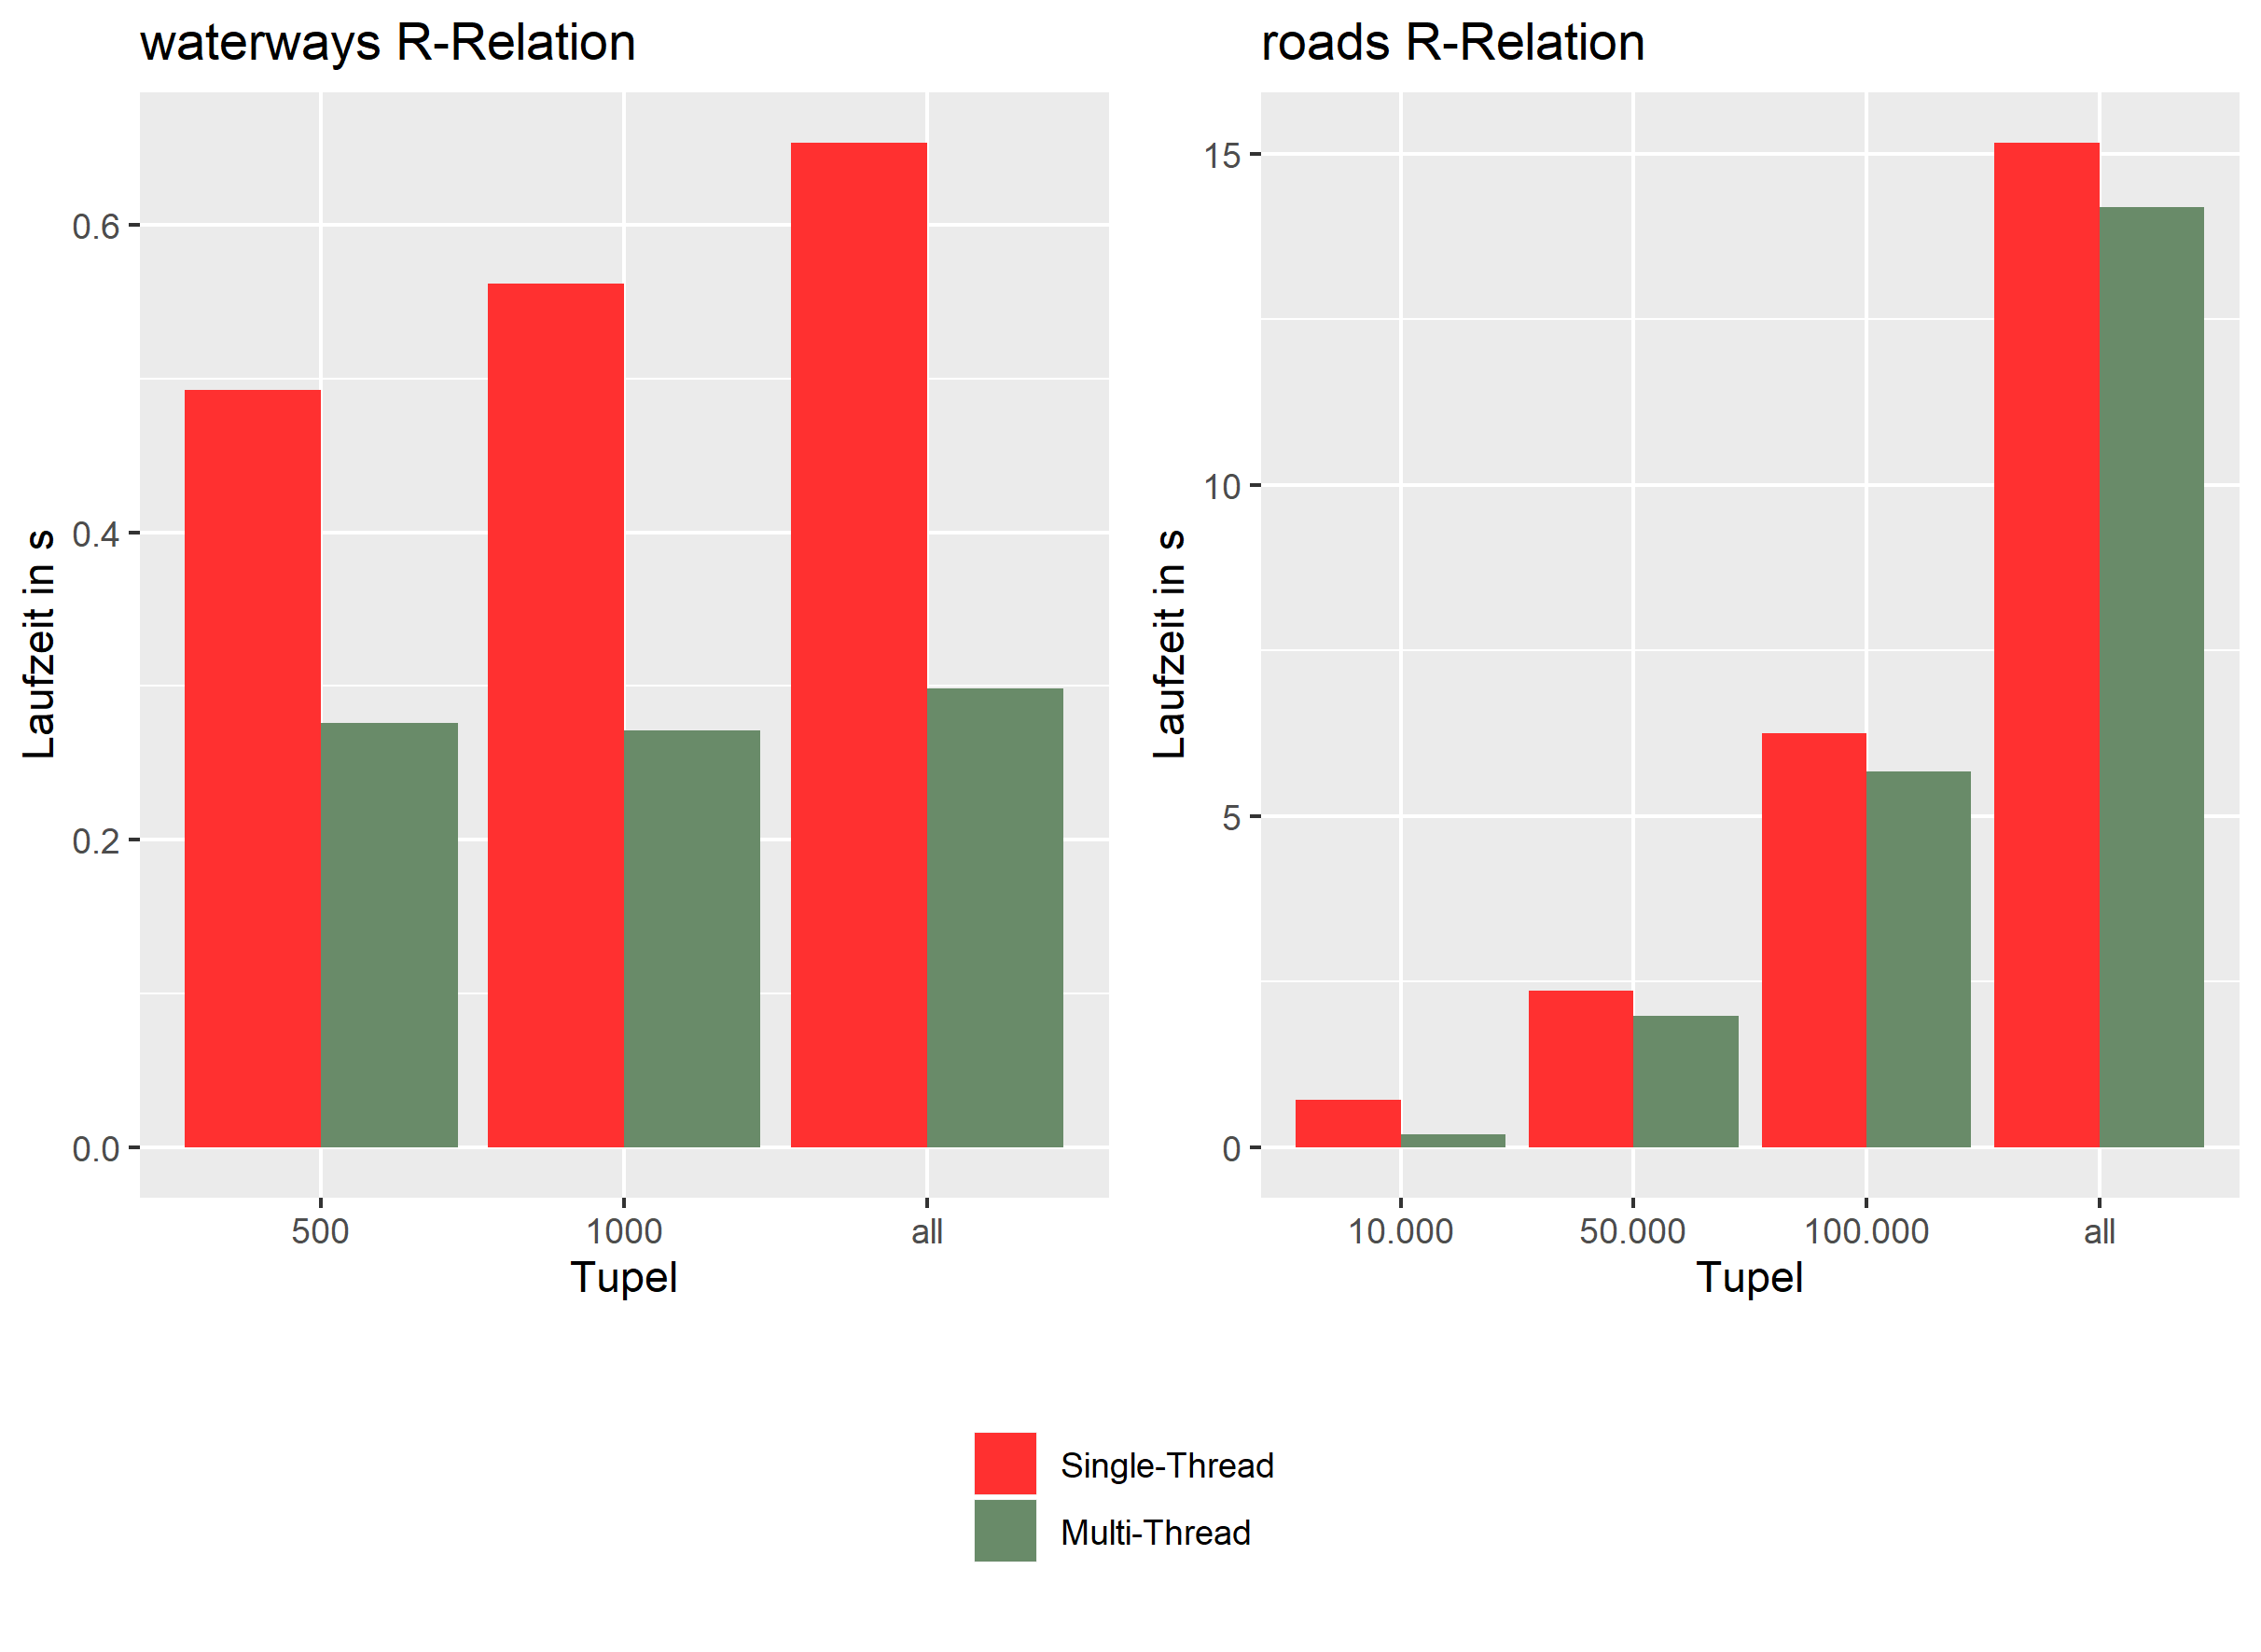
\includegraphics[width=0.6\textwidth]{Bilder/sj_head_wr.png}}}	
	\caption{Spatial-Joins mit unterschiedlichen Relationen und Relationsgrößen.}
	\label{img:sjExpHeadAllg}
\end{figure}

Effizienter ist der von mir implementierte Algorithmus lediglich bei kleinen Relationen, sowohl bezüglich der R- als auch der S-Relation. Bei dem Selfjoin, dessen Laufzeitanalyse in \autoref{img:sjHeadExpRr} dargestellt ist, ist der Anstieg der Laufzeit bei der Singlethread-Variante nahezu linear, bei der Multithread-Variante exponentiell. Also ist wahrscheinlich ungünstiger Entscheidungen bei der Implementierung des Algorithmus der Grund, weshalb die Performancevorteile bei kleinen Relationen bei deren Vergrößerung verloren gehen. Im Experiment, dessen Ergebnis in \autoref{img:sjHeadExpWr} dargestellt ist, wurden die R- sowie die S-Relation ausgetauscht und dann die Größe der R-Relation variiert. Die eine Relation, die die Wasserwege in Berlin darstellt, ist klein (2104 Tupel). In beiden Fällen ist der Anstieg der Laufzeit im Gegensatz zu großen Relationen noch vergleichbar mit der Singlethread-Variante und insgesamt ist die Laufzeit unter Nutzung mehrerer Kerne besser. 

\begin{figure}
	\centering
	\subfloat[nach verfügbarem Speicherplatz\label{img:sjMemExp}]{{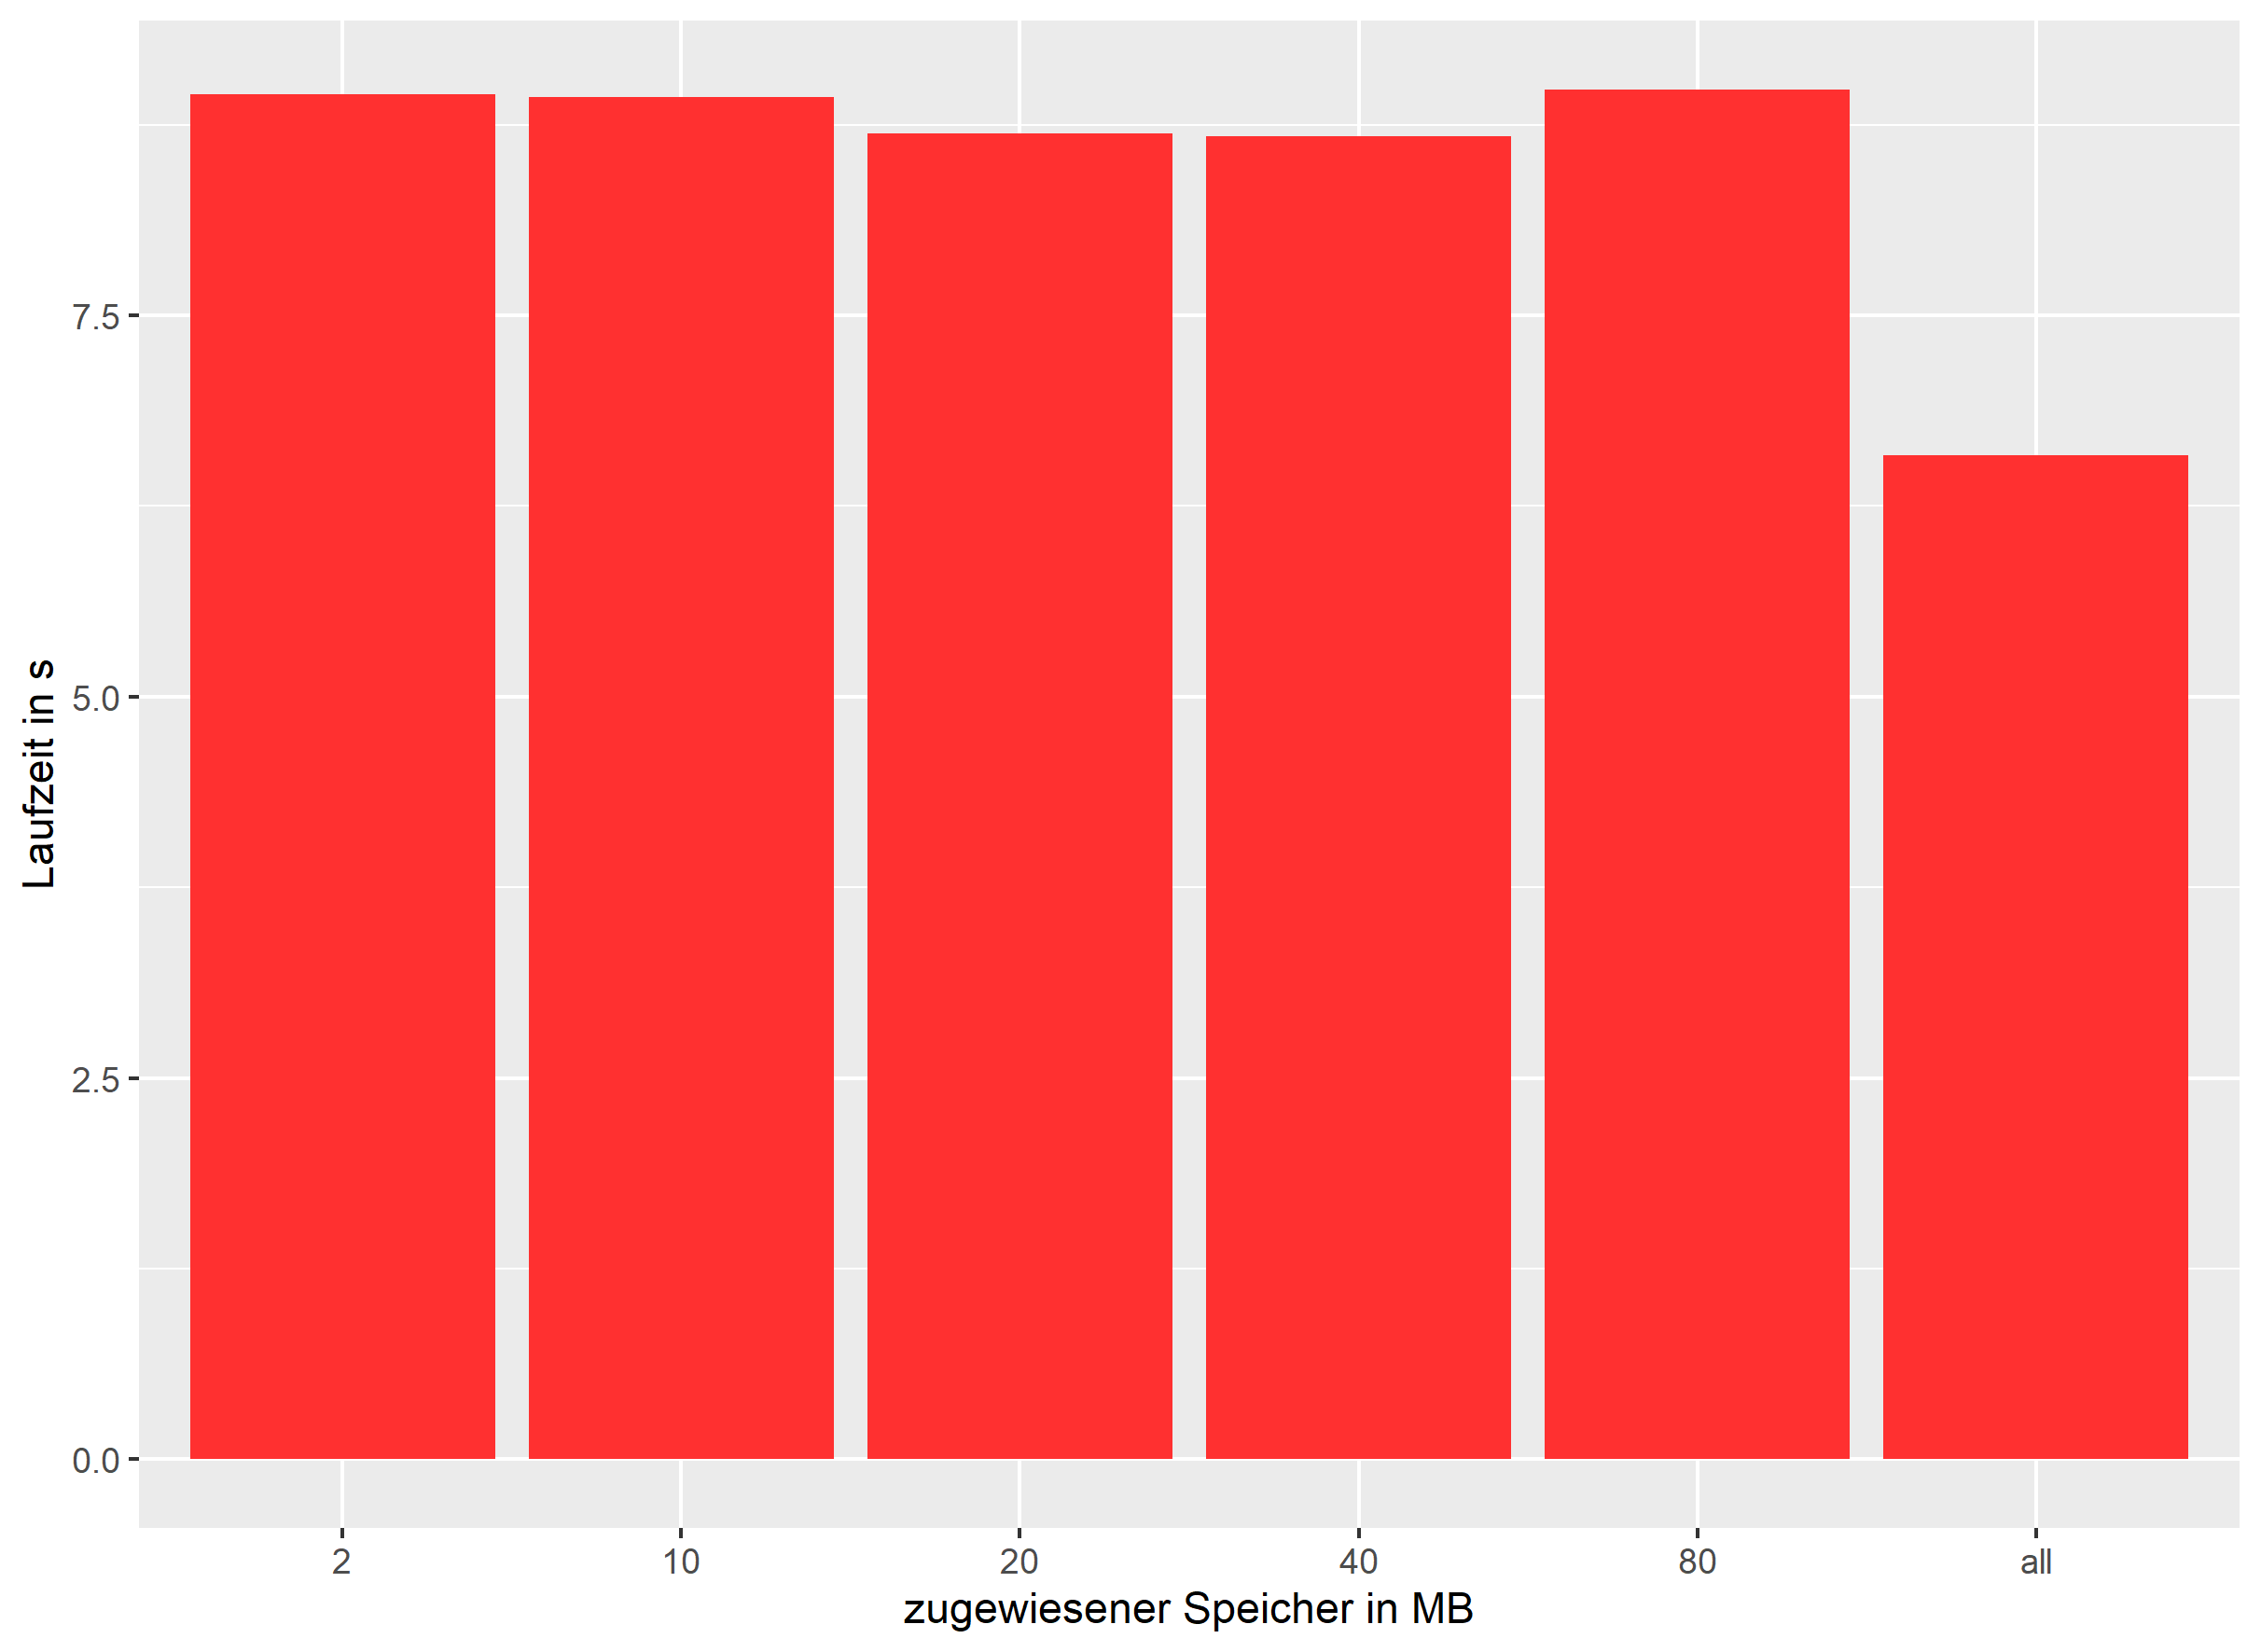
\includegraphics[width=0.45\textwidth]{Bilder/sj_mem.png}}}
	\subfloat[Konfiguration des R-Baums\label{img:sjTreeExp}]{{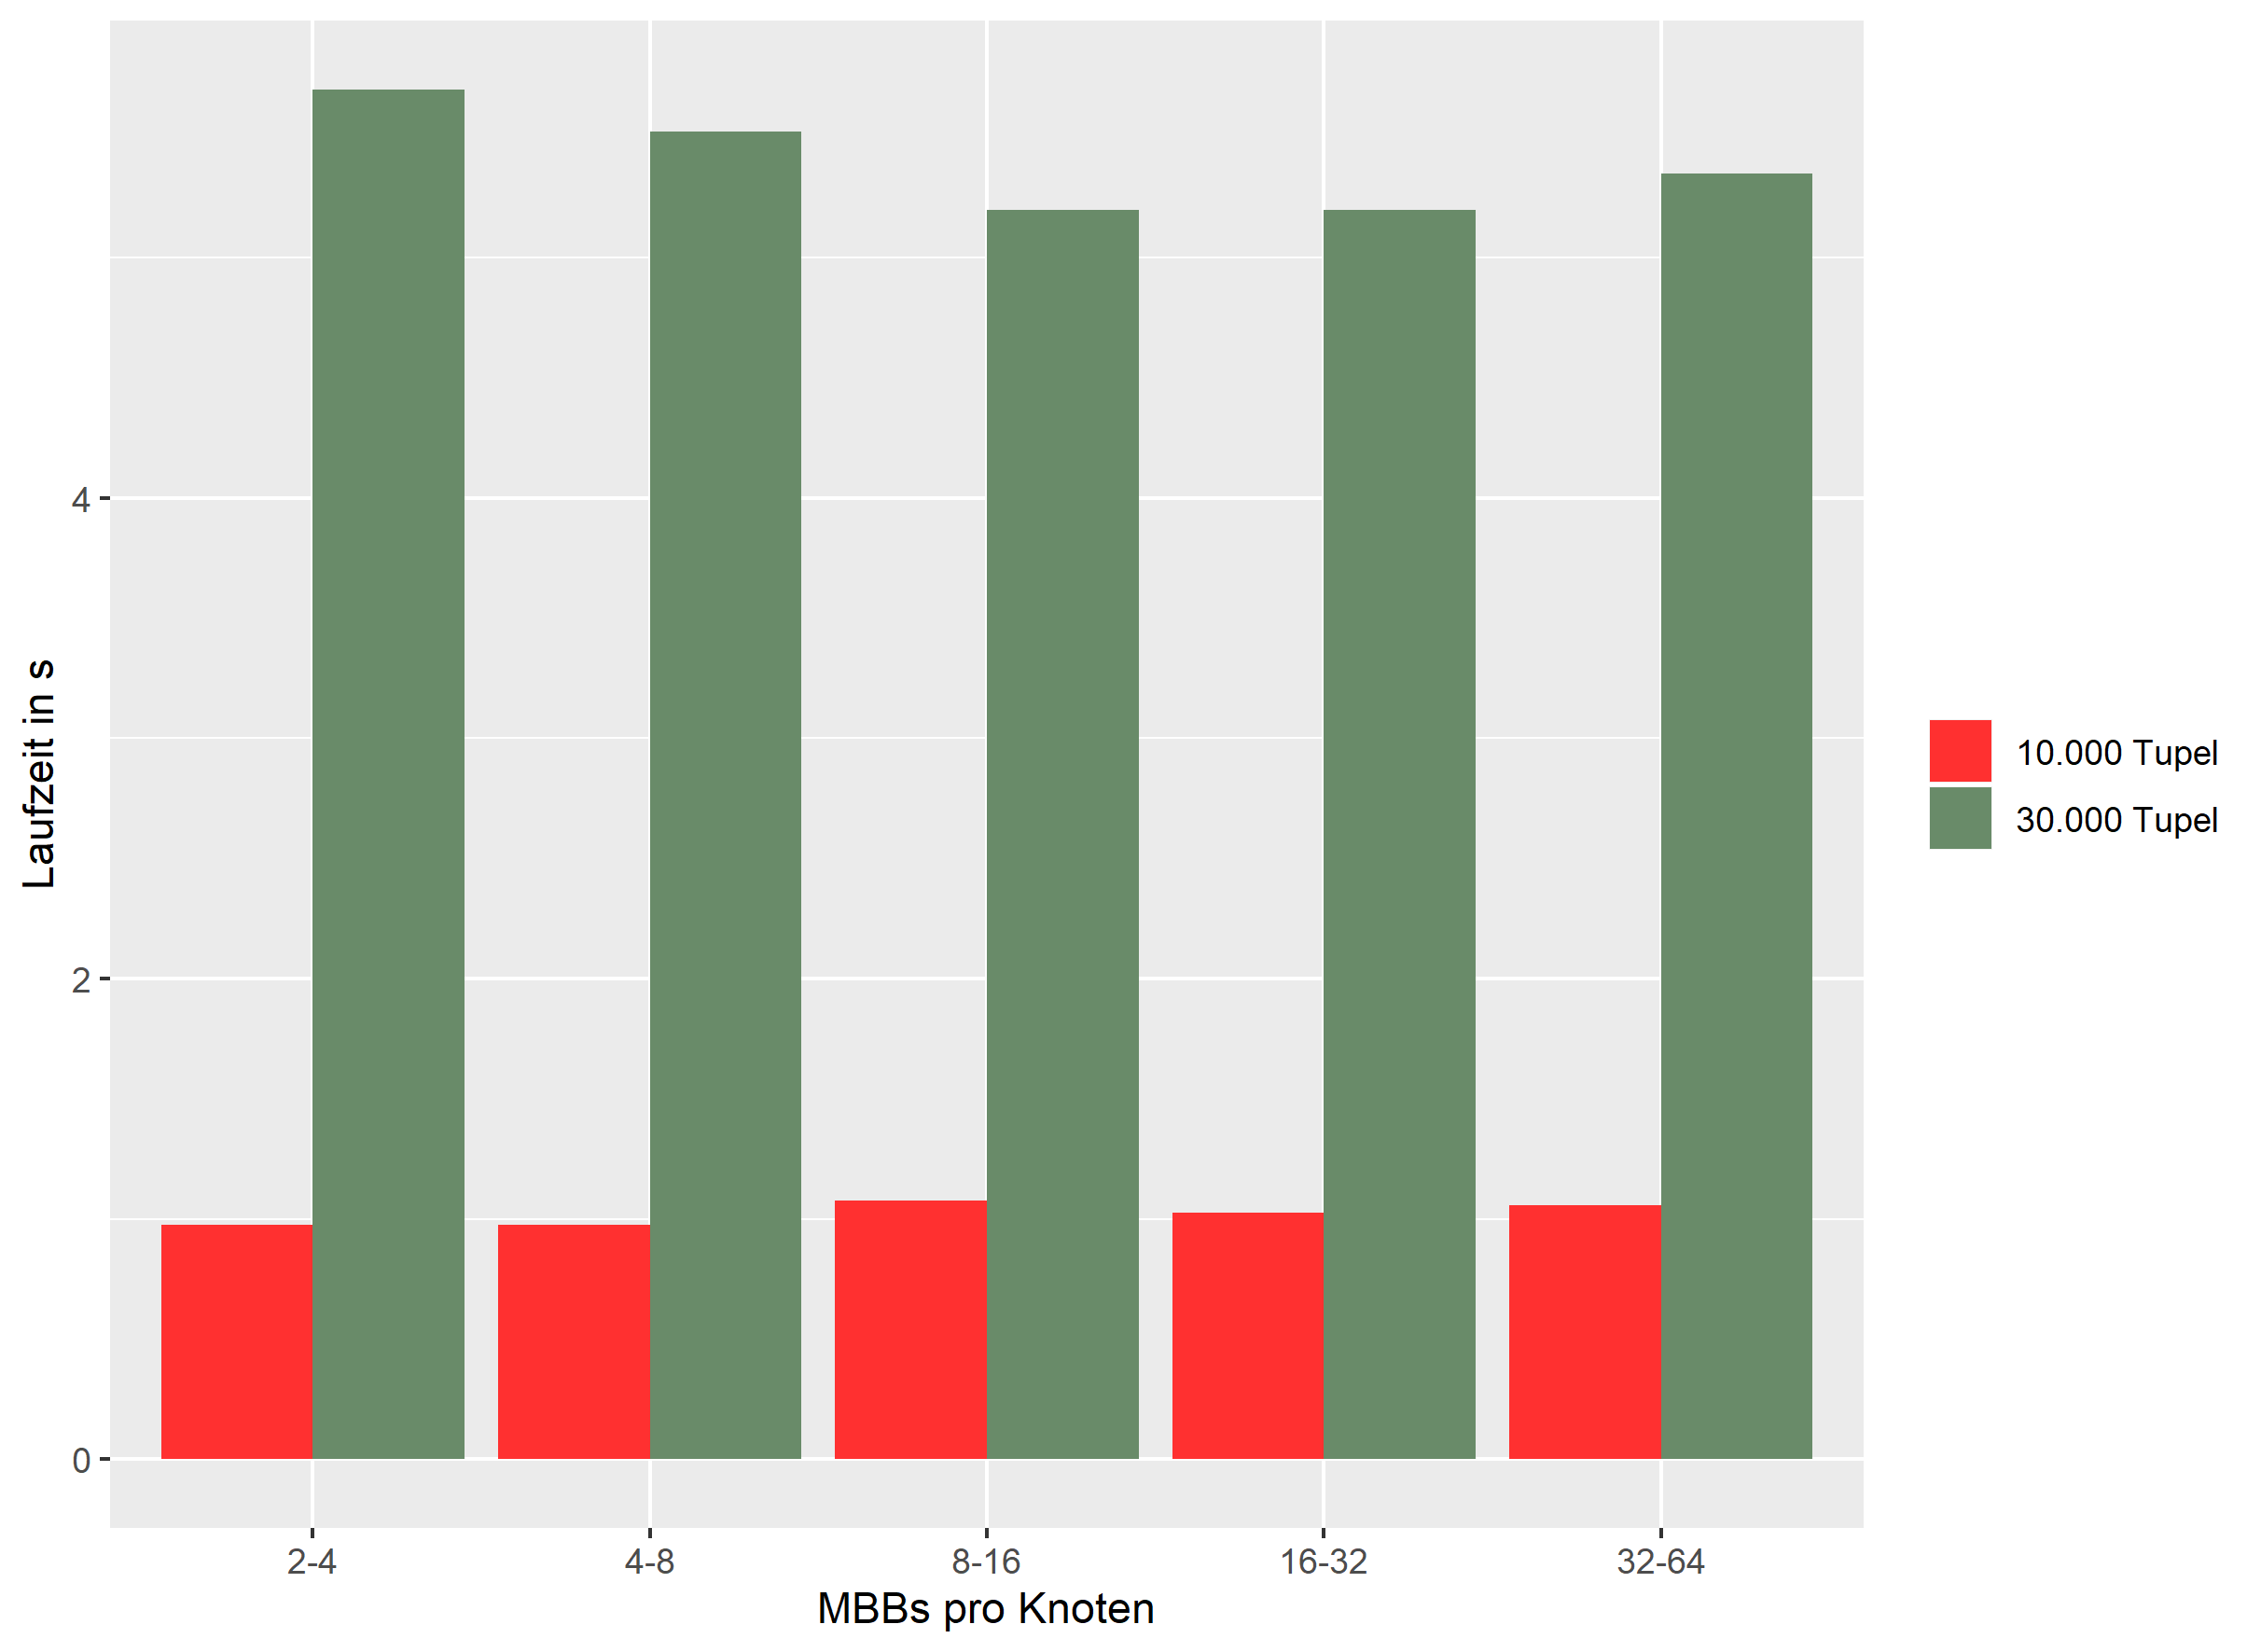
\includegraphics[width=0.45\textwidth]{Bilder/sj_tree.png}}}
	\caption{Verschiedene Experimente mit dem Spatial-Join.}
	\label{img:sjExpAllg}
\end{figure}

\autoref{img:sjMemExp} zeigt die Veränderung der Laufzeit, wenn der dem Operator zur Verfügung stehende Speicher reduziert wird. Hier gibt es nur eine sprunghafte Änderung zwischen 80~MB und dem Speicher, dem der Operator im Standardfall zur Verfügung steht. Der Operator benötigt Iterationen und muss Teile der R-Relation auslagern, wenn für die vollständige interne Struktur (also für die Tupel der R-Relation und den R-Baum) für diese Relation nicht genügend Speicher zur Verfügung steht. Hier ist das Verhalten des Operators merkwürdig, da bereits ab 80~MB keine Auslagerungsdateien mehr notwendig sind und bei 40~MB für jeden Thread nur eine Iteration notwendig ist, bei weniger Speicher mehr. Die I/O-Operationen sind also für den Operator nicht geschwindigkeitsbestimmend. Dies steht im Gegensatz dazu, dass zu Beginn vermutet wurde, dass gerade in einer Systemarchitektur mit geteiltem Permanentspeicher die I/O-Operationen das Nadelöhr sind, da hier kein paralleler Zugriff möglich ist. Dementsprechend muss bei dem Multithread-Spatial-Join die Bedeutung der CPU-Zeit für die Laufzeit deutlich dominieren.

Auch eine Konfiguration des R-Baums hat nur sehr wenig Auswirkung auf die Laufzeit. Für den In-Memory-R-Baum habe ich $2-4, 4-8, \ldots, 32-64$ Einträge pro Knoten gewählt. \autoref{img:sjTreeExp} zeigt, dass die Veränderung der Zahl der Einträge und damit der Höhe des Baums nur eine sehr geringe Auswirkung hat auf das Laufzeitverhalten. Wahrscheinlich wäre dies bei deutlich größeren Relationen anders, aber bei 10.000 bzw. 30.000 Tupel lohnt es nicht, den R-Baum beispielsweise über die Attribute des \Fb{mThreadedSpatialJoin}s parametrisierbar zu machen.   

\begin{figure}
	\centering
	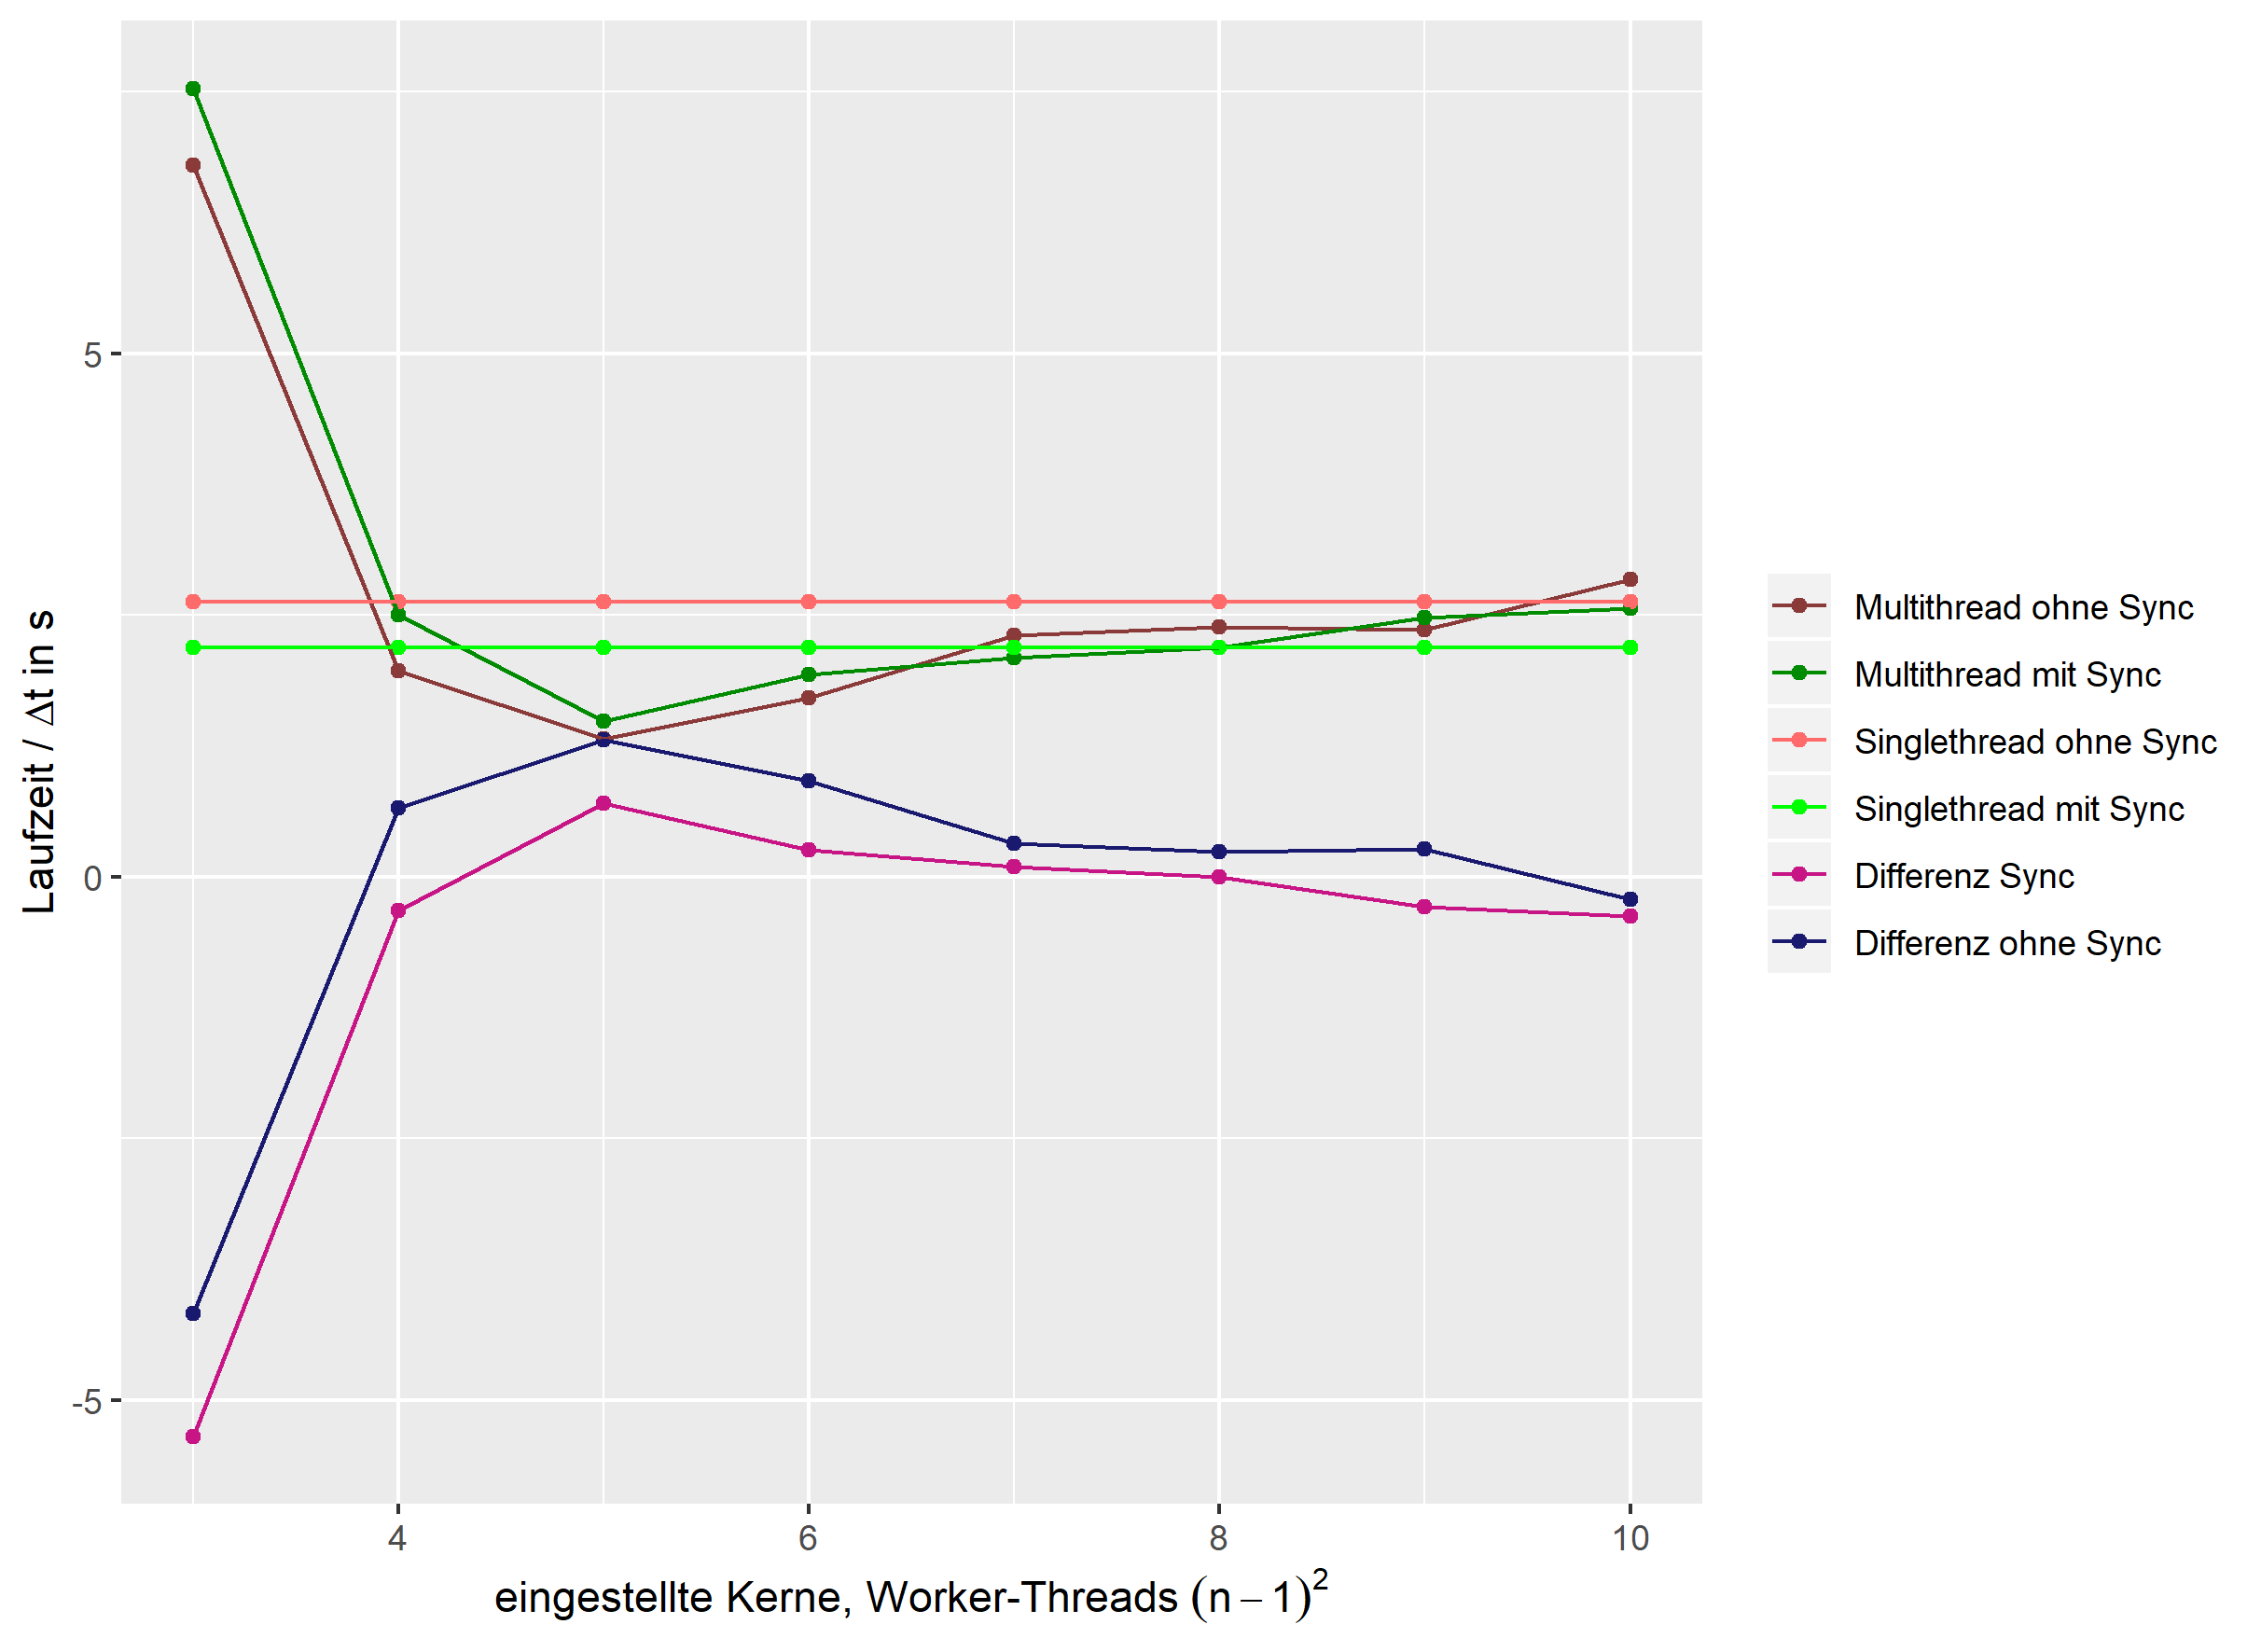
\includegraphics[width=0.6\textwidth]{Bilder/sj_nosync.png}
	\caption{Laufzeitverhalten nach Kernen mit und ohne Threadsicherheit: $pois \bowtie traf$.}
	\label{img:sjSync}
\end{figure}

\autoref{img:sjSync} zeigt signifikant, dass sogar bei Spatial-Joins mit wenig komplexen Objekten ohne Zugriffe auf \Fb{FLOBs} die Synchronisierung der Zugriffe auf die Speicherschicht einen sehr negativen Einfluss auf das Laufzeitverhalten eines Spatial-Joins hat. Pro $n-1$ genutzte Kerne werden $(n-1)^2$ Threads erzeugt. Insbesondere bei einer relativ geringen Threadzahl, die aber immer noch höher ist, als das System Kerne hat, fällt die Beschleunigung durch das Abschalten der Synchronisierung höher aus als bei der Single-Thread-Variante und ist immer deutlich. Von besonderem Interesse wäre es, die Auswirkung der viel aufwändigeren Synchronisation der Zugriffe des Flob-Managers zu beobachten, da ich hier einen bedeutenden Faktor für die schlechte Performance eines parallelen \Fb{Secondos} vermute und parallele Operatoren vor Allem bei aufwändigen Berechnungen sinnvoll sind, die meist \Fb{FLOBs} als Attribute verwenden. Nur leider funktioniert der parallele Zugriff auf \Fb{FLOBs} nicht ohne die Synchronisierung.   

\subsubsection{mThreadedFilter}
\label{entw:filter}

Eigentlich habe ich bei dem Filteroperator einen großen Performancegewinn erwartet, sofern die Prädikate einen hohen Rechenaufwand bedürfen, was bei Operationen mit komplexen räumlichen Typen der Fall ist. Allerdings zeigt der Operator ein eindeutig schlechteres Laufzeitverhalten als die Singlethread-Variante, und seine Laufzeit nimmt mit der Anzahl genutzter Kerne sogar ab. Interessant ist die Analyse dieses Operators vor allem, da sein eigentlicher Algorithmus sehr simpel ist und ich ungünstige Entscheidungen bei der Implementierung des Filters ausschließen kann. Der Algorithmus beruht vor allem auf der Auswertung eines Prädikats mithilfe von je einem Queryprozessor pro Thread.
  
Der Operator verwaltet seinen Speicher nicht selbst -- dementsprechend macht eine Analyse vom Laufzeitverhalten des zur Verfügung stehenden Speichers keinen Sinn. \autoref{img:filterHead} zeigt, dass der auf einem Kern ausgeführte Filter-Operator durchgehend schneller ist als die Multithread-Variante. Ausgewertet wurde ein komplexes Prädikat, welches auf Schnittpunkte zweier Linien prüft. Allerdings ist hier der Anstieg der Laufzeit beim Singlethread-Operator steiler. Da diese Entwicklung erst bei der letzten Messung sichtbar ist, ist jedoch eine sichere Vorhersage das Verhalten bei sehr großen Relationen nicht möglich. Eine Überprüfung ist auch nicht möglich, da der Operator wegen des Problems bei der Synchronisierung der Zugriffe auf die Berkeley-DB bei Relationen über 20.000 Tupeln nicht mehr stabil arbeitet. 

\begin{figure}
	\centering
	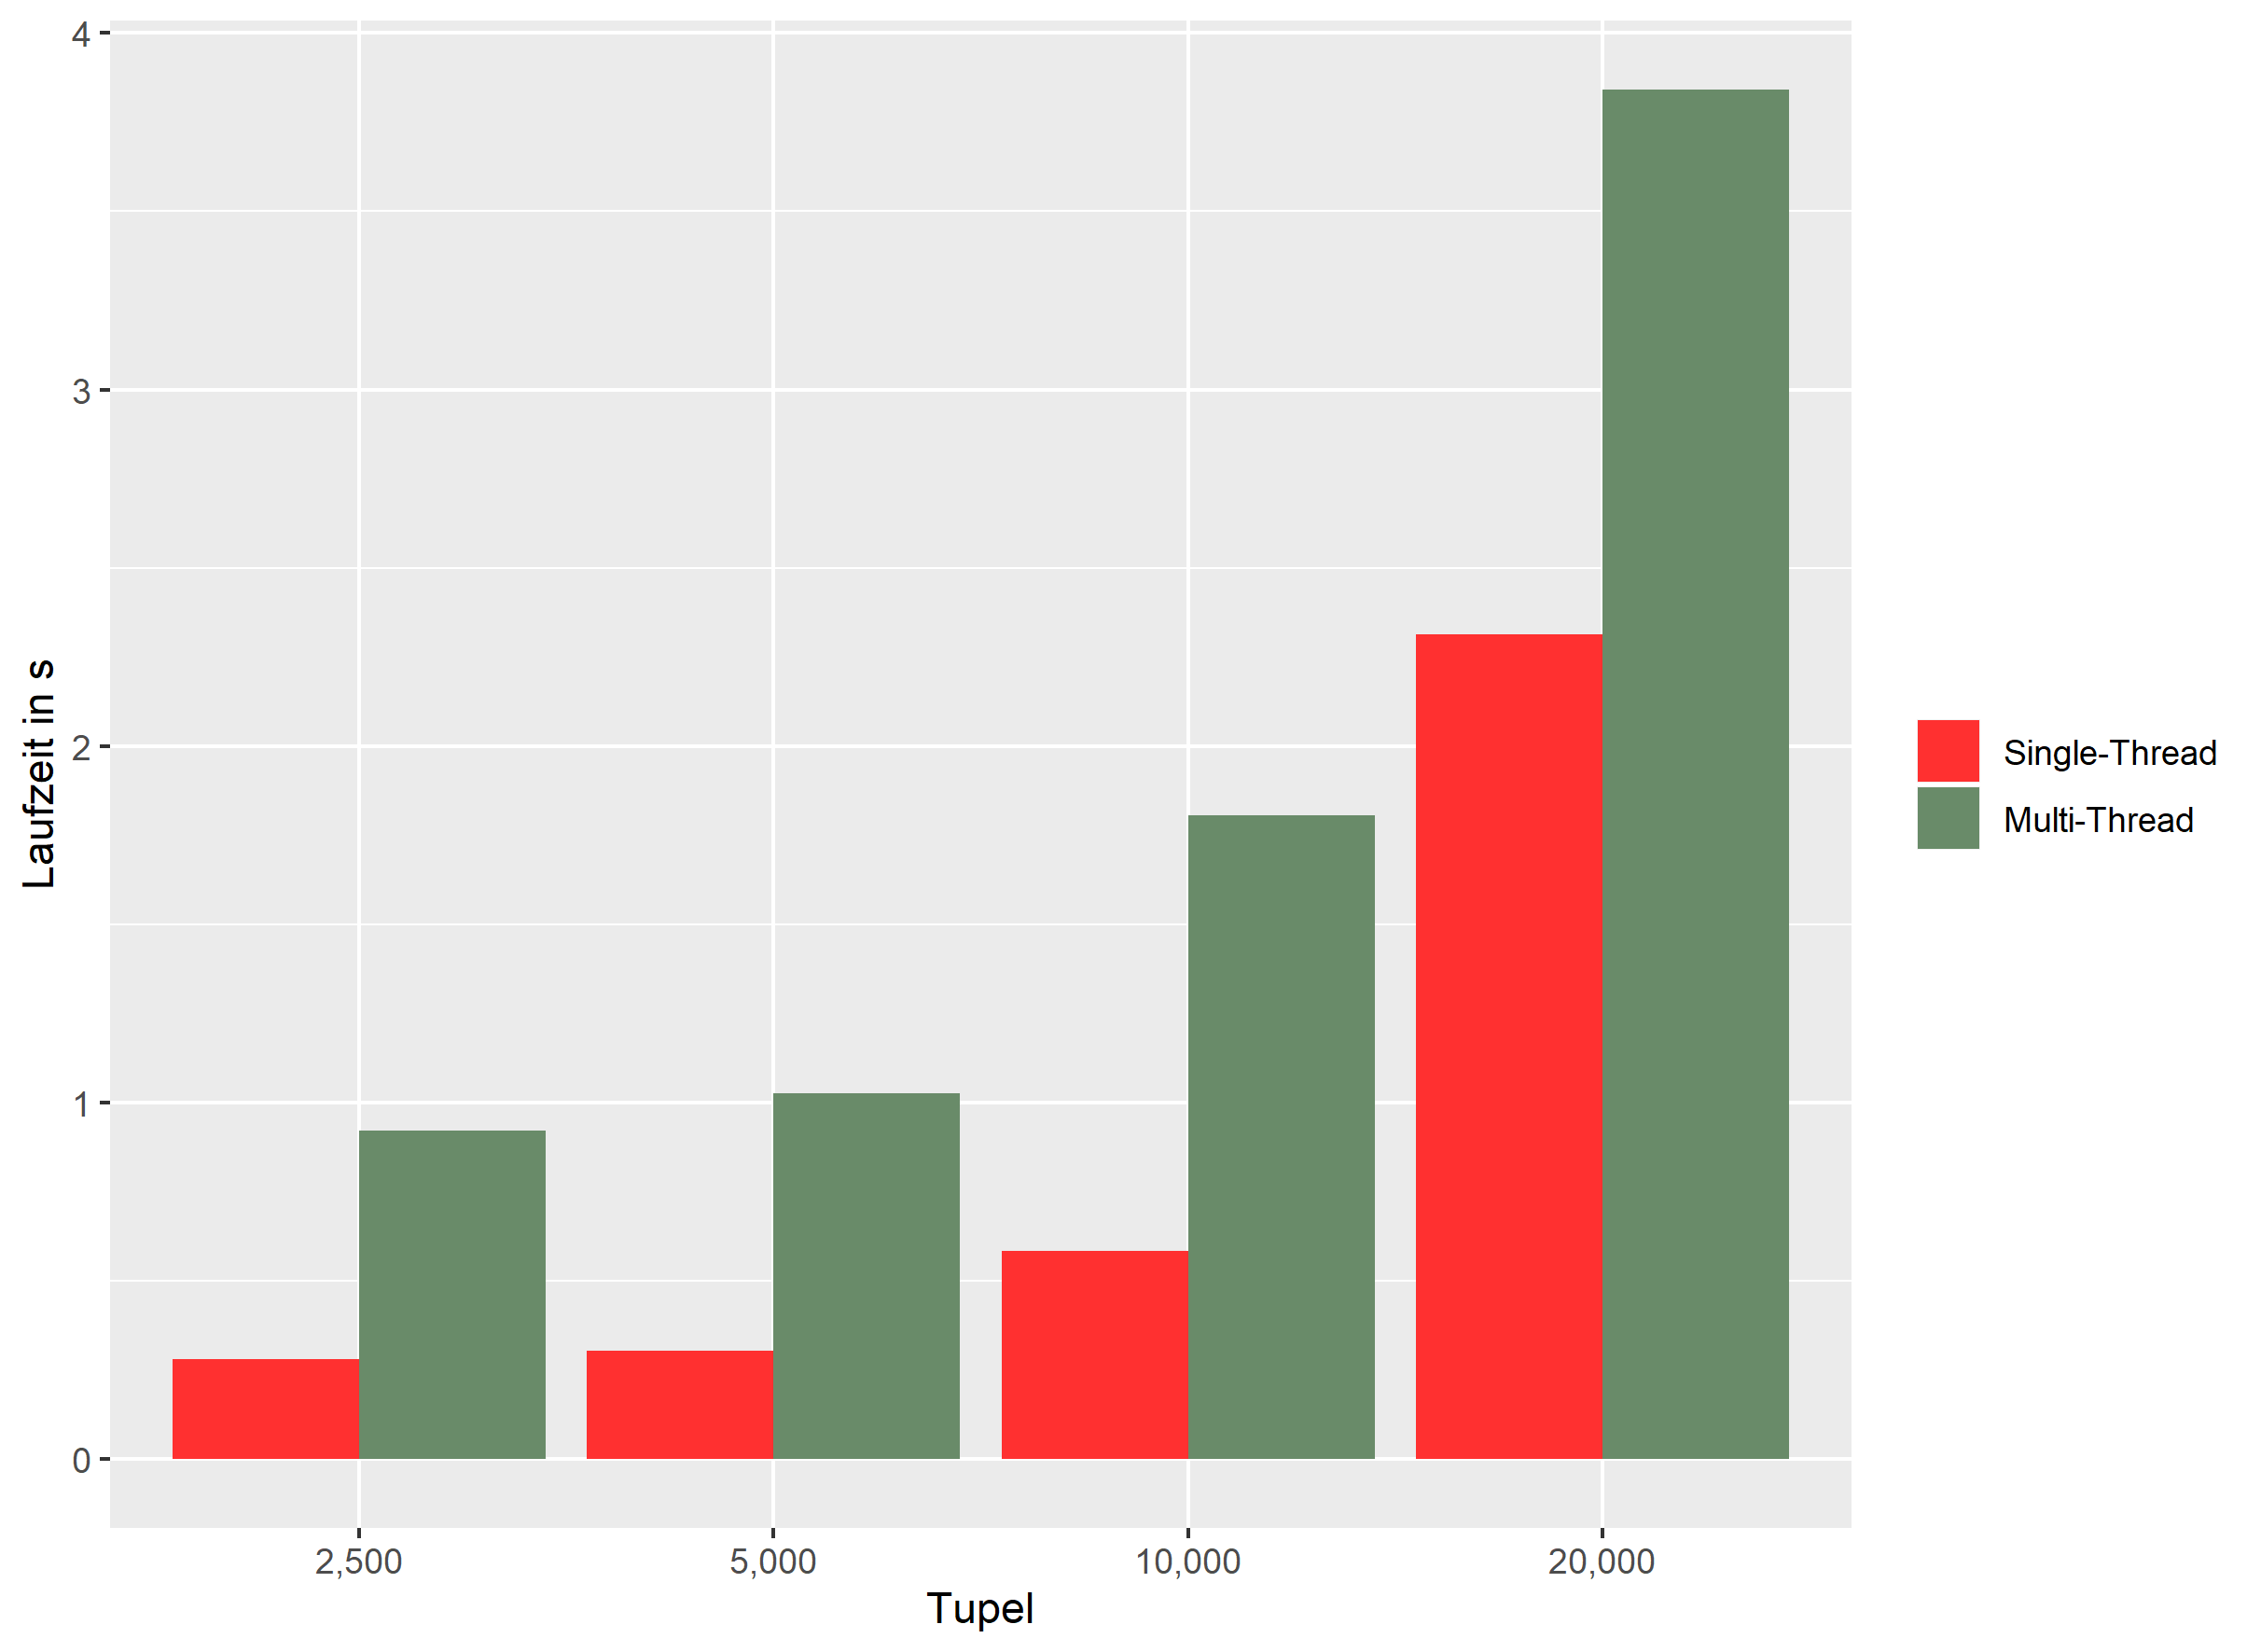
\includegraphics[width=0.60\textwidth]{Bilder/filter_head.png}
	\caption{Filter und verschiedene Relationsgrößen.}
	\label{img:filterHead}
\end{figure}

Da das Laufzeitverhalten deutlich hinter den Erwartungen zurückbleibt und eine un"-güns"-ti"-ge Implementierung der Auswertung der Prädikate ausgeschlossen werden kann, muss der Grund für die schlechte Performance entweder im Scheduling liegen oder in der Synchronisierung. In einem letzten Schritt wurde allerdings das Scheduling stark vereinfacht, indem die Tupelströme direkt in den Workern entgegengenommen werden. Eine erste Annahme, dass die Synchronisation des ursprünglich komplexen Scheduling mit einem hohen Synchronisationsaufwand das schlechte Laufzeitverhalten verursacht, kann also nicht bestätigt werden, auch wenn das neue vereinfachte Scheduling einen kleinen Laufzeitgewinn mit sich brachte. Die Warteschlange, die für das einsammeln der Ergebnistupel genutzt wird, benötigt eine Synchronisierung über Locks -- allerdings müsste bei einer Verringerung der Anzahl an Ergebnissen im Verhältnis zur Relationsgröße sich dann das Laufzeitverhalten verbessern, was nicht signifikant der Fall ist. Eine weitere Erklärung für die schlechte Performance der Multithread-Operatoren sind die Synchronisierungen im \Fb{Secondo}-Kern, vor allem bei Zugriffen auf \Fb{FLOBs}, die bei den Auswertungen der Prädikate stattfinden (und bei anderen Operatoren auch beim Auslagern von Daten inklusive ihrer \Fb{FLOBs}). Eine gute Performance lässt sich also wahrscheinlich nur erreichen, wenn versucht wird, die Operatoren so anzulegen, dass teure Synchronisierungen nur selten eingesetzt werden müssen. Auch wenn hier noch einige Optimierungen möglich sind, zum Beispiel mit der Verwendung von je einer eigenen Ergebniswarteschlange für jeden Thread, aus den alternierend ausgelesen wird, ist wahrscheinlich ein wirklich performantes Multithreading-\Fb{Secondo} nur möglich, wenn parallele Zugriffe auf die Speicherschicht des Datenbanksystems zugelassen werden. Eine Verbesserung der Synchronisierung der \Fb{FLOBs} ist zwingend notwendig, da ein paralleles \Fb{Secondo} ohne \Fb{FLOBs}, die parallel bisher nicht stabil nutzbar sind, wenig Sinn macht. Hier allerdings weiterhin auf umfangreiche Locks oder teure Nachrichten zu setzen, ist nicht vielversprechend, da sich die Performanceprobleme paralleler Zugriffe auf die Speicherschicht weiter verschärfen würden. 

\section{Fazit}

Eine Bewertung der Implementierung einer Algebra für Multithread-Versionen ausgewählter Operatoren erfolgt anhand der in \autoref{problem} gesetzten Ziele. Eine Implementierung je einer parallelen Version der Operatoren Sort, Equi-Join und Spatial-Join erfolgte, wobei ich den Spatial-Joins in einen Filter- und des Refinement-Schritt unterteilt habe. Alle Operatoren der \Fb{mThreadedAlgebra} führen mit mindestens drei zugewiesenen Kernen in den meisten Fällen zu korrekten Ergebnissen, allerdings mit deutlichen Einschränkungen bei der Verwendung von \Fb{FLOBs}. Die meisten Operatoren arbeiten auch korrekt, wenn mehr Threads zugewiesen werden als dem System zur Verfügung stehen. Alle Operatoren haben mindestens den gleichen Funktionsumfang wie die entsprechende Singlethread-Versionen. Beim Spatial-Join-Operator ist es darüber hinaus noch möglich, die Minimal Bounding Box um das Joinattribut zu vergrößern, so dass sich dieser auch als Filter-Schritt für räumliche Verschmelzungen eignet, deren Prädikate einen Abstand der im Prädikat verwendeten räumlichen Objekte voraussetzen, wie zum Beispiel Joins nach Nachbarschaften. Einzig der Hash-Join liefert unter bestimmten Bedingungen kein korrektes Ergebnis: Er ignoriert Tupelpaare, wenn ein Joinattribut so häufig mit einem gleichen Hashwert auftritt, dass das entsprechende Bucket nicht mehr in den Hauptspeicher passt. Hier wäre ein Abbruch des Operators sinnvoller, da in diesem Fall ein Hash-Join ein sehr schlechtes Laufzeitverhalten hat und dementsprechend nicht mehr sinnvoll ist.

Die zweite und sehr deutliche Einschränkung der Robustheit ist ein grundsätzliches Problem des \Fb{Secondo}-Kerns in der Synchronisation der Zugriffe auf die Berkeley-DB bzw. die Einschränkung des \Fb{Secondo}-Datenbanksystems, durch den Storage-Manager keine parallelen Zugriffe auf die Berkeley-DB zuzulassen. Sofern \Fb{FLOBs} verwendet werden, reicht die bisherige Synchronisierung nicht aus, die vor allem im Flob-Manager stattfindet, so dass abhängig davon, wie häufig die \Fb{FLOBs} in den Hauptspeicher geladen werden müssen, Zeiger auf SMI-Files oder Locks korrupt werden, die zu Abstürzen oder Deadlocks im Queryabschluss führen können. Hier habe ich erfolglos versucht, die Synchronisation des \Fb{Secondo}-Kerns zu verbessern. Die Fehler im Kern, die die Entwicklung eines parallelen \Fb{Secondos} einschränken, konnten eingegrenzt werden, aber nicht vollumfänglich identifiziert worden. Folgende Schritte sind wahrscheinlich notwendig, um sinnvoll parallele Operatoren für \Fb{Secondo} implementieren zu können: Weitere Teile der Speicherschicht des Kerns müssen mit Locks versehen werden. Zugriffe unterschiedlicher Module auf die unterste Speicherschicht von \Fb{Secondo} müssen untereinander synchronisiert werden und nicht nur einzelne Module intern wie der Flob-Manager. Da Synchronisierungen immer deutliche Performanceeinbußen bedeuten, insbesondere wenn sie nicht nur sehr wenig rechenaufwändige Bereiche betreffen, wäre es der beste Weg, den \Fb{Secondo}-Kern so zu verändern, dass die Berkeley-DB für einen parallelen Zugriff konfiguriert werden kann. 

Nicht erreicht wurde auch das Ziel, dass die Operatoren effizienter als ihre Singlethread-Varianten sind. Lediglich der Spatial-Join-Operator ist unter bestimmten Bedingungen schneller als die Variante, die nur mit einem Kern arbeitet, allerdings mit der Einschränkung, dass sich das Laufzeitverhalten bei großen Relationen schneller verschlechtert als bei der Singlethread-Version. Also gerade bei sehr großen Relationen ist die von mir implementierte Variante nicht mehr konkurrenzfähig. Die Versuche, einerseits die entstehenden Fehler, die bei der Verwendung von \Fb{FLOBs} auftreten, zu identifizieren und andererseits Lösungen zu entwickeln, haben sehr viel Zeit in Anspruch genommen, so dass zum Schluss eine Optimierung der Operatoren nicht in dem Maße erfolgen konnte, wie sie notwendig gewesen wären. Da parallele Operatoren gerade bei komplexen und umfangreichen Daten sinnvoll sind, habe ich der korrekten Verarbeitung von \Fb{FLOBs} eine hohe Priorität zugewiesen und auch in der Entwicklung Korrektheit und Robustheit vor Effizienz betrachtet.

Im folgenden fasse ich die Gründe zusammen, die für die mangelnde Effizienz der von mir implementierten Operatoren verantwortlich sind. Bei zwei Operatoren, dem Spatial-Join und dem Hash-Join, habe ich aufgrund eines exponentiellen Wachstums der Laufzeit bezüglich der Relationsgröße, der nicht bei den Singlethread-Varianten auftritt, Fehler in der Entwicklung des verwendeten Algorithmus gemacht. Allerdings habe ich auch deutliche Probleme beobachtet, die nicht nur einzelne Operatoren betreffen und zum Teil nicht in meiner Implementierung begründet sind, sondern im \Fb{Secondo}-Kern:

\begin{itemize}
	\item Scheduling aufwändig mit hohem Synchronisationsaufwand.
	\item Synchronisation in den Datenstrukturen für den Datenaustausch zwischen den Threads.
	\item Synchronisation und damit Serialisierung beim Zugriff auf persistierte Daten, vor allem auf \Fb{FLOBs}.
	\item Allgemein höhere Kosten der Synchronisation als erwartet. Vor allem Bedingungsvariablen teuer und entstehende Wartezeiten in Threads.
	\item Entkopplung der Threads klappt in den meisten Fällen nicht -- dementsprechend blockierenden Threads bis zum Terminierung.
	\item Geteilter Arbeitsspeicher zwischen den Threads -- insbesondere bei einer ungünstigen Verteilung von Daten kann es sogar vorkommen, dass bereits bei kleineren Datenmengen persistiert werden muss.
	\item Eine Partitionierung zerstört eventuell Vorsortierungen, die im Operator ausgenutzt werden könnten.
	\item Teils sind die in den Threads vorgenommen Berechnungen pro Tupel nicht aufwändig genug, um die Kosten für das Overhead der Parallelisierung zu rechtfertigen.
	\item I/O-Zugriffe finden nicht parallel statt, da nur eine Festplatte verwendet wird. Allerdings ist die Auswirkung hiervon anders als erwartet recht gering, zumindest bei der Verwendung von schnellen SSDs.
\end{itemize}
 
Abschließend kann ich zusammenfassend feststellen, dass eine Implementierung eines parallelen \Fb{Secondos} nur sinnvoll gelingen kann, wenn das Problem mit dem parallelen Zugriff auf \Fb{FLOBs} gelöst wird. Eine weitere Synchronisierung ist hier meiner Meinung nach kein sinnvoller Ansatz, da er die Kosten der Parallelisierung weiter erhöht, sondern ein paralleler Zugriff auf die Speicherschicht muss ermöglicht werden. Allerdings gäbe es wahrscheinlich noch Verbesserungspotentiale in meiner Implementierung, die zumindest die meisten hier entwickelten Operatoren in bestimmten Einsatzkontexten konkurrenzfähig machen würden. Bei einer Verbesserung müssen die Kosten für Synchronisation und Scheduling, aber auch die Einschränkungen, die der \Fb{Secondo}-Kern hier vorgibt, im gleichen Ausmaß betrachtet werden wie der Entwurf des Algorithmus. Gerade die Kosten der Synchronisierung wurden von mir unterschätzt.

\pagebreak 
\printbibliography[notcategory=nicht-in-bib]


\end{document}
